\documentclass[]{book}
\usepackage{lmodern}
\usepackage{amssymb,amsmath}
\usepackage{ifxetex,ifluatex}
\usepackage{fixltx2e} % provides \textsubscript
\ifnum 0\ifxetex 1\fi\ifluatex 1\fi=0 % if pdftex
  \usepackage[T1]{fontenc}
  \usepackage[utf8]{inputenc}
\else % if luatex or xelatex
  \ifxetex
    \usepackage{mathspec}
  \else
    \usepackage{fontspec}
  \fi
  \defaultfontfeatures{Ligatures=TeX,Scale=MatchLowercase}
\fi
% use upquote if available, for straight quotes in verbatim environments
\IfFileExists{upquote.sty}{\usepackage{upquote}}{}
% use microtype if available
\IfFileExists{microtype.sty}{%
\usepackage{microtype}
\UseMicrotypeSet[protrusion]{basicmath} % disable protrusion for tt fonts
}{}
\usepackage{hyperref}
\hypersetup{unicode=true,
            pdftitle={The medfate reference book},
            pdfborder={0 0 0},
            breaklinks=true}
\urlstyle{same}  % don't use monospace font for urls
\usepackage{natbib}
\bibliographystyle{apalike}
\usepackage{color}
\usepackage{fancyvrb}
\newcommand{\VerbBar}{|}
\newcommand{\VERB}{\Verb[commandchars=\\\{\}]}
\DefineVerbatimEnvironment{Highlighting}{Verbatim}{commandchars=\\\{\}}
% Add ',fontsize=\small' for more characters per line
\usepackage{framed}
\definecolor{shadecolor}{RGB}{248,248,248}
\newenvironment{Shaded}{\begin{snugshade}}{\end{snugshade}}
\newcommand{\KeywordTok}[1]{\textcolor[rgb]{0.13,0.29,0.53}{\textbf{#1}}}
\newcommand{\DataTypeTok}[1]{\textcolor[rgb]{0.13,0.29,0.53}{#1}}
\newcommand{\DecValTok}[1]{\textcolor[rgb]{0.00,0.00,0.81}{#1}}
\newcommand{\BaseNTok}[1]{\textcolor[rgb]{0.00,0.00,0.81}{#1}}
\newcommand{\FloatTok}[1]{\textcolor[rgb]{0.00,0.00,0.81}{#1}}
\newcommand{\ConstantTok}[1]{\textcolor[rgb]{0.00,0.00,0.00}{#1}}
\newcommand{\CharTok}[1]{\textcolor[rgb]{0.31,0.60,0.02}{#1}}
\newcommand{\SpecialCharTok}[1]{\textcolor[rgb]{0.00,0.00,0.00}{#1}}
\newcommand{\StringTok}[1]{\textcolor[rgb]{0.31,0.60,0.02}{#1}}
\newcommand{\VerbatimStringTok}[1]{\textcolor[rgb]{0.31,0.60,0.02}{#1}}
\newcommand{\SpecialStringTok}[1]{\textcolor[rgb]{0.31,0.60,0.02}{#1}}
\newcommand{\ImportTok}[1]{#1}
\newcommand{\CommentTok}[1]{\textcolor[rgb]{0.56,0.35,0.01}{\textit{#1}}}
\newcommand{\DocumentationTok}[1]{\textcolor[rgb]{0.56,0.35,0.01}{\textbf{\textit{#1}}}}
\newcommand{\AnnotationTok}[1]{\textcolor[rgb]{0.56,0.35,0.01}{\textbf{\textit{#1}}}}
\newcommand{\CommentVarTok}[1]{\textcolor[rgb]{0.56,0.35,0.01}{\textbf{\textit{#1}}}}
\newcommand{\OtherTok}[1]{\textcolor[rgb]{0.56,0.35,0.01}{#1}}
\newcommand{\FunctionTok}[1]{\textcolor[rgb]{0.00,0.00,0.00}{#1}}
\newcommand{\VariableTok}[1]{\textcolor[rgb]{0.00,0.00,0.00}{#1}}
\newcommand{\ControlFlowTok}[1]{\textcolor[rgb]{0.13,0.29,0.53}{\textbf{#1}}}
\newcommand{\OperatorTok}[1]{\textcolor[rgb]{0.81,0.36,0.00}{\textbf{#1}}}
\newcommand{\BuiltInTok}[1]{#1}
\newcommand{\ExtensionTok}[1]{#1}
\newcommand{\PreprocessorTok}[1]{\textcolor[rgb]{0.56,0.35,0.01}{\textit{#1}}}
\newcommand{\AttributeTok}[1]{\textcolor[rgb]{0.77,0.63,0.00}{#1}}
\newcommand{\RegionMarkerTok}[1]{#1}
\newcommand{\InformationTok}[1]{\textcolor[rgb]{0.56,0.35,0.01}{\textbf{\textit{#1}}}}
\newcommand{\WarningTok}[1]{\textcolor[rgb]{0.56,0.35,0.01}{\textbf{\textit{#1}}}}
\newcommand{\AlertTok}[1]{\textcolor[rgb]{0.94,0.16,0.16}{#1}}
\newcommand{\ErrorTok}[1]{\textcolor[rgb]{0.64,0.00,0.00}{\textbf{#1}}}
\newcommand{\NormalTok}[1]{#1}
\usepackage{longtable,booktabs}
\usepackage{graphicx,grffile}
\makeatletter
\def\maxwidth{\ifdim\Gin@nat@width>\linewidth\linewidth\else\Gin@nat@width\fi}
\def\maxheight{\ifdim\Gin@nat@height>\textheight\textheight\else\Gin@nat@height\fi}
\makeatother
% Scale images if necessary, so that they will not overflow the page
% margins by default, and it is still possible to overwrite the defaults
% using explicit options in \includegraphics[width, height, ...]{}
\setkeys{Gin}{width=\maxwidth,height=\maxheight,keepaspectratio}
\IfFileExists{parskip.sty}{%
\usepackage{parskip}
}{% else
\setlength{\parindent}{0pt}
\setlength{\parskip}{6pt plus 2pt minus 1pt}
}
\setlength{\emergencystretch}{3em}  % prevent overfull lines
\providecommand{\tightlist}{%
  \setlength{\itemsep}{0pt}\setlength{\parskip}{0pt}}
\setcounter{secnumdepth}{5}
% Redefines (sub)paragraphs to behave more like sections
\ifx\paragraph\undefined\else
\let\oldparagraph\paragraph
\renewcommand{\paragraph}[1]{\oldparagraph{#1}\mbox{}}
\fi
\ifx\subparagraph\undefined\else
\let\oldsubparagraph\subparagraph
\renewcommand{\subparagraph}[1]{\oldsubparagraph{#1}\mbox{}}
\fi

%%% Use protect on footnotes to avoid problems with footnotes in titles
\let\rmarkdownfootnote\footnote%
\def\footnote{\protect\rmarkdownfootnote}

%%% Change title format to be more compact
\usepackage{titling}

% Create subtitle command for use in maketitle
\providecommand{\subtitle}[1]{
  \posttitle{
    \begin{center}\large#1\end{center}
    }
}

\setlength{\droptitle}{-2em}

  \title{The medfate reference book}
    \pretitle{\vspace{\droptitle}\centering\huge}
  \posttitle{\par}
    \author{true}
    \preauthor{\centering\large\emph}
  \postauthor{\par}
      \predate{\centering\large\emph}
  \postdate{\par}
    \date{2019-05-29}

\usepackage{booktabs}
\usepackage{amsthm}
\makeatletter
\def\thm@space@setup{%
  \thm@preskip=8pt plus 2pt minus 4pt
  \thm@postskip=\thm@preskip
}
\makeatother

\begin{document}
\maketitle

{
\setcounter{tocdepth}{1}
\tableofcontents
}
\hypertarget{part-preliminaries}{%
\part{Preliminaries}\label{part-preliminaries}}

\hypertarget{intro}{%
\chapter{Introduction}\label{intro}}

Being able to anticipate the impact of global change on ecosystems is one of the major environmental challenges in contemporary societies. However, uncertainties in how ecological systems function and practical constraints in how to integrate available information prevent the development of robust and reliable predictive models. Despite the amount of knowledge accumulated about the functioning and dynamics of Mediterranean forests, scientists should make coordinate their efforts to address the challenge of integrating the different global change drivers in a modelling framework useful for research and applications.

The R package \texttt{medfate} has been designed to study the characteristics and simulate dynamics of Mediterranean forests. Fire and drought impacts are the main drivers covered by the package. Representation of vegetation is not spatially-explicit (i.e.~trees or shrubs do not have explicit coordinates within forest stands). This simplified representation is chosen so that package functions can be easily applied to forest plot data from national forest inventories. Since the package intends to facilitate predictions of not only forest functioning but also forest structure and composition, the taxonomic identity of plants is stored, and parameter values need to be provided for each taxonomic entity (but the package could be used with functional groups).

\hypertarget{package-installation}{%
\section{Package installation}\label{package-installation}}

Package \textbf{medfate} can be found at \href{https://CRAN.R-project.org/package=medfate}{CRAN}, where it is updated every few months. Hence, it can be installed using:

\begin{Shaded}
\begin{Highlighting}[]
\KeywordTok{install.packages}\NormalTok{(}\StringTok{"medfate"}\NormalTok{)}
\end{Highlighting}
\end{Shaded}

Users can also download and install the latest stable versions GitHub as follows (required package \texttt{devtools} should be installed/updated first):

\begin{Shaded}
\begin{Highlighting}[]
\NormalTok{devtools}\OperatorTok{::}\KeywordTok{install_github}\NormalTok{(}\StringTok{"miquelcaceres/medfate"}\NormalTok{)}
\end{Highlighting}
\end{Shaded}

When installing from GitHub, may need to force the installation of package vignettes, by using:

\begin{Shaded}
\begin{Highlighting}[]
\NormalTok{devtools}\OperatorTok{::}\KeywordTok{install_github}\NormalTok{(}\StringTok{"miquelcaceres/medfate"}\NormalTok{, }
                         \DataTypeTok{build_opts =} \KeywordTok{c}\NormalTok{(}\StringTok{"--no-resave-data"}\NormalTok{, }\StringTok{"--no-manual"}\NormalTok{))}
\end{Highlighting}
\end{Shaded}

\hypertarget{how-to-use-this-book}{%
\section{How to use this book}\label{how-to-use-this-book}}

This is a reference book for simulation and static models included in \textbf{medfate}. Hands-on user guides can be found as package vignettes included in its distribution. The manual is intended to reflect \textbf{version 0.8.2}. Our purpose is to continuously update this reference with package updates, so that users can know about the models they are using at the time when functions are run. As the manual will keep package updates, after model applications users should store the PDF version of the reference manual to be sure it matches the version the package reported in the application (e.g.~report or article).

\hypertarget{model-inputs}{%
\chapter{Model inputs}\label{model-inputs}}

\hypertarget{soil-description}{%
\section{Soil description}\label{soil-description}}

Soil can be described using between 1 and 5 soil layers. For each soil layer \(s\) the following physical parameters are needed for each soil layer (see function \texttt{defaultSoilParams()}):

\begin{itemize}
\tightlist
\item
  \(Z_{s}\) {[}\texttt{widths}{]}: Soil layer width (\(d_s\), in mm).
\item
  \(P_{clay,s}\) {[}\texttt{clay}{]}: Percent of clay.
\item
  \(P_{sand,s}\) {[}\texttt{sand}{]}: Percent of sand.
\item
  \(OM\) {[}\texttt{om}{]}: Percentage of organic mater per dry weight (can be missing).
\item
  \(BD_{s}\) {[}\texttt{bd}{]}: Bulk density (g/cm3) of each soil layer.
\item
  \(P_{rocks,s}\) {[}\texttt{rfc}{]}: Percentage of rock fragment content (\(P_{rocks,s}\)).
\end{itemize}

Soil texture (i.e.~percent of sand, silt and clay), bulk density and rock fragment content can differ between soil layers. Specifying a deep rocky layer is important because Mediterranean plants may extend their roots into cracks existing in the parent rock \citep{Ruffault2013}. For those users lacking soil information, package \textbf{medfate} provides a function to get soil information from \href{https://soilgrids.org/}{SoilGrids.org} (see function \texttt{soilgridsParams()}).

\hypertarget{water-retention-curves}{%
\subsection{Water retention curves}\label{water-retention-curves}}

Water retention curve of a soil layer \(s\) is the relationship between the water content, \(\theta_s\) (in \(m^3 \cdot m^{-3}\) of soil, excluding rock fragments), and the soil water potential, \(\Psi_s\) (in MPa). This curve is characteristic for different types of soil, and is also called the soil moisture characteristic curve. Two water retention curve models are provided:

\begin{enumerate}
\def\labelenumi{\arabic{enumi}.}
\tightlist
\item
  \emph{Saxton model}: In this model, volumetric soil moisture \(\theta(\Psi_s)\) corresponding to a given water potential \(\Psi\) (in MPa) below \(\Psi_{fc}\) is calculated using:
  \begin{equation}\theta(\Psi) = (\Psi/A)^{(1/B)}\end{equation}
  where \(A\) and \(B\) depend on the texture and, if available, organic matter in the soil layer. If organic matter is available, \(A\) and \(B\) are calculated \(P_{clay}\), \(P_{sand}\) and \(OM\) following \citet{Saxton2006}. Otherwise, they are calculated from \(P_{clay}\) and \(P_{sand}\) as indicated in \citet{Saxton1986}. Volumetric changes between field capacity and saturation are estimated using a linear function.
\item
  \emph{Van Genuchten model}: The well known van Genuchten {[}@-Genuchten1980{]} model is:
  \begin{equation}\theta(\Psi) = \theta_{res}+\frac{\theta_{sat}-\theta_{res}}{\left[1+ (\alpha \cdot \Psi)^n \right]^{1-1/n}}\end{equation}
  where \(\theta(\psi)\) is the water retention, \(\theta_{sat}\) is the saturated water content, \(\theta_{res}\) is the residual water content, \(\alpha\) is related to the inverse of the air entry pressure (and here has to be expressed in MPa\(^{-1}\)), and \(n\) is a measure of the pore-size distribution.
\end{enumerate}

\hypertarget{soil-initialization}{%
\subsection{Soil initialization}\label{soil-initialization}}

Soil initialization is needed to estimate soil hydrological parameters from its physical description. Initialization is done using function \texttt{soil()}, which adds the following information to the physical soil description:

\begin{itemize}
\tightlist
\item
  \(P_{macro, s}\) {[}\texttt{macro}{]}: Percentage of macroporosity corresponding to each soil layers. Macroporosity values are calculated for each soil layer using the equations given in \citet{Stolf2011}.
\item
  \(\gamma_{soil}\) {[}\texttt{Gsoil}{]}: The maximum daily evaporation from soil(\(mm \cdot day^{-1}\)).
\item
  \(\kappa_{soil}\) {[}\texttt{Ksoil}{]}: Extinction parameter to regulate the amount of water extracted from each soil layer during bare soil evaporation.
\item
  \(n_{s}\), \(\alpha_{s}\), \(\theta_{sat,s}\),\(\theta_{res,s}\) {[}\texttt{VG\_n}, \texttt{VG\_alpha}, \texttt{VG\_theta\_sat}, \texttt{VG\_theta\_res}{]}: Parameter of the Van Genuchten-Mualem equations.
\end{itemize}

Parameters of the van Genuchten-Mualem model are estimated from the physical description of the soil using two kinds of pedotransfer functions (see help for \texttt{soil()}):

\begin{enumerate}
\def\labelenumi{\arabic{enumi}.}
\tightlist
\item
  Using the USDA texture classification and the average texture class parameters given by \citet{Carsel1988}.
\item
  Directly from the soil texture, organic matter and bulk density, using the pedotransfer functions in \citet{Toth2015}.
\end{enumerate}

\hypertarget{water-holding-capacity-and-water-table-depth}{%
\subsection{Water holding capacity and water table depth}\label{water-holding-capacity-and-water-table-depth}}

Soil water holding capacity (\(V_s\), in mm) in soil layer \(s\) is defined as the volumetric water content at field capacity:
\begin{equation}
V_s = d_s\cdot ((100-P_{rocks,s})/100)\cdot\theta_{fc,s}
\end{equation}
where \(d_s\) is the depth of the soil layer (in mm) and \(P_{rocks,s}\) is the percentage of rock fragments. Thus, soil water holding capacity depends on the water retention curve used to determine \(\theta_{fc} = \theta(-0.033)\). Soil water content at saturation is calculated anagolously, but replacing \(\theta_{fc,s}\) by \(\theta_{sat,s}\). Similarly water content at wilting point (-1.5 MPa) is calculated replacing \(\theta_{fc,s}\) by \(\theta_{wp,s}\) where \(\theta_{wp} = \theta(-1.5)\). The amount of extractable water is difference between water content at field capacity and a the water content at a minimum water potential, which can be set at wilting point or lower values (by default at -5 MPa).

Water table depth (\(WT\), in mm) equals soil depth when all soil layers are below field capacity. When some layers are between field capacity and saturation, water table depth is calculated as:
\begin{equation}
WT = \sum_{s}{d_s \cdot \min\left[1,(\theta_{sat,s} - \theta(\Psi_s))/(\theta_{sat,s}-\theta_{fc,s})\right]}
\end{equation}

\hypertarget{vegetation-description}{%
\section{Vegetation description}\label{vegetation-description}}

Vegetation in the stand is described using a set of plant cohorts, in an object
of class \texttt{spwbInput}. Each plant cohort \(i\) is primarly defined by its
species identity (\(SP_i\); with R name {[}\texttt{SP}{]}).

\hypertarget{aboveground-parameters}{%
\subsection{Aboveground parameters}\label{aboveground-parameters}}

The aboveground structure if each cohort is defined using the following attributes:

\begin{itemize}
\tightlist
\item
  \(H_i\) {[}\texttt{H}{]}: Total tree or shrub height (in cm).
\item
  \(CR_i\) {[}\texttt{CR}{]}: Crown ratio (i.e.~the ratio between crown length and
  total height).
\item
  \(LAI^{live}_i\) {[}\texttt{LAI\_live}{]}: (Maximum) leaf area index (one-side
  leaf area of plants in the cohort per surface area of the stand).
\item
  \(LAI^{dead}_i\) {[}\texttt{LAI\_dead}{]}: Dead leaf area index (one-side dead
  leaf area of plants in the cohort per surface area of the stand).
\item
  \(LAI^{\phi}_i\) {[}\texttt{LAI\_expanded}{]}: Current expanded leaf area index (one-side expanded
  leaf area of plants in the cohort per surface area of the stand).
\end{itemize}

All vegetation characteristics stay constant during water balance simulations, although the actual expanded leaf area and dead leaf area may vary is the species is winter deciduous.

\hypertarget{belowground-parameters}{%
\subsection{Belowground parameters}\label{belowground-parameters}}

The root system of each plant cohorts is described using the proportion of fine
roots in each soil layer:

\begin{itemize}
\tightlist
\item
  \(v_{i,s}\) {[}\texttt{V}{]}: The proportion of fine roots in each soil layer \(s\).
\end{itemize}

The rooting system of each cohort \(i\) (i.e.~the proportions \(v_{i,s}\)) can be defined assuming conic distribution of fine roots (see \texttt{root\_conicDistribution()}). In this case, only rooting depth parameter is needed to determine fine root proportions. Alternatively, one can adopt the linear dose response model (Collins and Bras, 2007; Schenk and Jackson, 2002):
\begin{equation}
Y_i(z)=\frac{1}{1+(z/Z_{50,i})^{c_i}}
\end{equation}
where \(Y_i(z)\) is the cumulative fraction of fine root mass located between surface and depth \(z\); \(Z_{50,i}\) is the depth above which 50\% of the root mass is located; and \(c_i\) is a shape parameter related to \(Z_{50,i}\) and \(Z_{95,i}\) as \(c_i = 2.94 / \ln(Z_{50,i} / Z_{95,i})\) (see \texttt{root\_ldrDistribution()}).

\begin{figure}
\centering
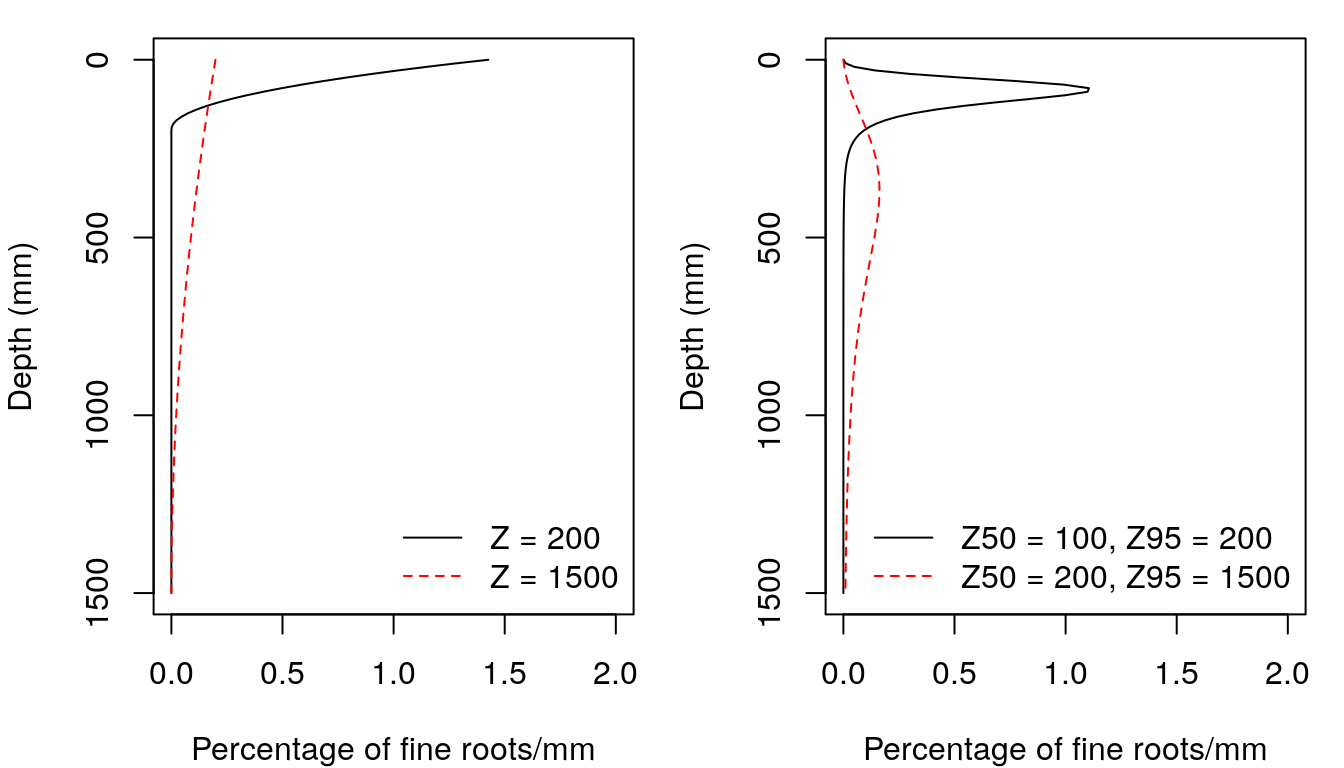
\includegraphics{medfatebook_files/figure-latex/unnamed-chunk-3-1.pdf}
\caption{\label{fig:unnamed-chunk-3}Examples of root density profile according to a conic distribution (left) and the linear dose response model (right).}
\end{figure}

\hypertarget{part-basic-water-balance-modelling}{%
\part{Basic water balance modelling}\label{part-basic-water-balance-modelling}}

\hypertarget{basic-water-balance-model}{%
\chapter{Basic water balance model}\label{basic-water-balance-model}}

\hypertarget{design-principles}{%
\section{Design principles}\label{design-principles}}

The water balance model described in \citet{DeCaceres2015} calculates temporal variations in soil moisture on a daily step basis for the input forest stand and for the period corresponding to input weather data.

The model considers only the vertical spatial dimension of the stand and not the horizontal distribution of
plants within it. In other words, the model is not spatially explicit (i.e., plants do not interact for space explicitly). Still, the stand is divided into groups of plants, here referred to as \emph{plant cohorts} of different species, height and leaf area index (\(LAI\)). Height and \(LAI\) values determine competition for light. \(LAI\) values also drive competition for water, along with root distribution. The soil water balance follows the design principles of SIERRA \citep{Mouillot2001, Ruffault2014, Ruffault2013} and BILJOU \citetext{\citealp{Granier1999}; \citeyear{Granier2007}}, although some features are taken from other models \citep{Kergoat1998}. Potential evapotranspiration (\(PET\)) is given as input and the model determines maximum canopy transpiration (\(Tr_{\max}\)) using an empirical relationship between the \(LAI\) of the stand and the ratio \(Tr_{\max}/PET\) \citep{Granier1999}. Actual plant transpiration is estimated using a function that depends on current soil moisture levels, species-specific drought resistance, fine root distribution and the degree of shading of the target plant cohort.

\hypertarget{state-variables}{%
\section{State variables}\label{state-variables}}

The model has the following state variables:

\begin{itemize}
\tightlist
\item
  Cumulative growth degree days, \(GDD\), are tracked by the model and determine leaf phenological status of winter deciduous species.
\item
  Daily soil moisture content dynamics on each layer \(s\) are tracked using \(W_s = \theta(\Psi_s)/ \theta_{fc,s}\), the \textbf{proportion of volumetric soil moisture in relation to field capacity}, where field capacity, \(\theta_{fc,s}\), is assumed to correspond to \(\Psi_{fc} = -0.033\) MPa. Note that \(W_s\) values larger than one are possible if the soil is between field capacity and saturation (which can happen if deep drainage is not allowed).
\item
  If snow accumulation/melting is considered, the model tracks \(S_{snow}\), the snow water equivalent (in mm) of the snow pack storage over the surface.
\item
  If irreversible cavitation is activated, the model tracks \(P_{embolized,i}\), the maximum value of daily drought stress so far experienced.
\end{itemize}

\hypertarget{water-balance}{%
\section{Water balance}\label{water-balance}}

Daily variations in soil water content (mm) can be summarized as:

\begin{equation}
\Delta{SWC} = Pr + Sm - In - Ru - Dd - Es -Tr
\end{equation}

where \(Pr\) is precipitation as rainfall, \(Sm\) is water from melting the snow pack (if considered), \(In\) is the interception loss (i.e., water evaporated after being intercepted by the canopy), \(Ru\) is surface runoff, \(Dd\) is deep drainage (i.e.~water percolated to layers beyond soil depth), \(Es\) is evaporation from soil and \(Tr\) is plant transpiration. If snow dynamics are considered, the water balance of the snow pack is defined as:

\begin{equation}
\Delta{S_{snow}} = Ps - Sm
\end{equation}

where \(Ps\) is precipitation as snowfall and \(Sm\) is snow melt.

\hypertarget{process-scheduling}{%
\section{Process scheduling}\label{process-scheduling}}

Every day water balance is perfomed as follows. The model first updates leaf area values according to the phenology of species and calculates light extinction. After that, the model updates soil water content of soil layers in several steps:

\begin{itemize}
\tightlist
\item
  If snow dynamics are included, increase snow pack from snow precipitation (\(Ps\)) and decreases it from snow melting (\(Sm\)) (section \ref{snowpack})
\item
  Increase soil moisture due to rainfall (\(Pr\)), surface runon (\(Ro\)) and snow melting (\(Sm\)), after accounting for interception loss (\(In\)), surface runoff (\(Ru\)) and deep drainage (\(Dd\)) (sections \ref{interception} and \ref{runoff})
\item
  Decrease water content due to bare soil evaporation (\(Es\)).
\item
  Determine transpiration, photosynthesis and drought stress for each plant cohort (section \ref{transpirationgranier}) and decrease water content due to plant transpiration (\(Tr\)).
\end{itemize}

\hypertarget{model-input}{%
\section{Model input}\label{model-input}}

\hypertarget{metereological-input}{%
\subsection{Metereological input}\label{metereological-input}}

Weather input data must include variables calculated at the \textbf{daily} scale.

\begin{itemize}
\tightlist
\item
  \(T_{mean}\) {[}\texttt{MeanTemperature}{]}: Mean daily temperature (in \(^{\circ} \mathrm{C}\)).
\item
  \(Rad\) {[}\texttt{Radiation}{]}: Solar radiation, after accounting for clouds (in \(MJ \cdot m^{-2}\)), only necessary if snow pack dynamics are simulated (i.e., if \texttt{snowpack = TRUE}).
\item
  \(P\) {[}\texttt{Precipitation}{]}: Daily precipitation (in \(L \cdot m^{-2}\) = mm of water).
\item
  \(PET\) {[}\texttt{PET}{]}: Daily potential evapotranspiration (in \(L \cdot m^{-2}\) = mm of water), preferably calculated using Penman's equation.
\end{itemize}

Optionally, the user may also specify values of wind speed (\(u\), in m·s\(^{-1}\), \texttt{WindSpeed}) that are used to control leaf fall in autumn. We recommend meteorological input to be generated using package \textbf{meteoland} \citep{DeCaceres2018}.

\hypertarget{control-parameters}{%
\subsection{Control parameters}\label{control-parameters}}

Control parameters are a list of parameter values, initialized using function \texttt{defaultControl()}, that the user can modify to change the general behavior of the model. The control values relevant for the simple water balance model are:

\begin{itemize}
\tightlist
\item
  \texttt{verbose\ {[}=TRUE{]}}: Whether extra console output is desired during simulations.
\item
  \texttt{soilFunctions\ {[}=\ "SX"{]}}: Water retention curve model, either ``SX'' (for Saxton) or ``VG'' (for Van Genuchten).
\item
  \texttt{snowpack\ {[}=\ TRUE{]}}: Whether dynamics of snow pack are included.
\item
  \texttt{drainage\ {[}=\ TRUE{]}}: Whether water exceeding the field capacity of the bottom layer is lost by deep drainage into a non-reachable compartment.
\item
  \texttt{transpirationMode\ {[}=\ "Granier"{]}}: Transpiration model, in this case ``Granier''.
\item
  \texttt{defaultWindSpeed\ {[}=\ 5{]}}: Default value for wind speed (in \(m \cdot s^{-1}\)) when this is missing (only used for leaf fall).
\item
  \texttt{cavitationRefill\ {[}=\ TRUE{]}}: If \texttt{FALSE} the model operates in a irreversible cavitation mode.
\end{itemize}

\hypertarget{model-output}{%
\section{Model output}\label{model-output}}

Function \texttt{spwb} returns a list object whose elements are data tables. Each table has dates as rows and has different output variables:

\begin{itemize}
\tightlist
\item
  \texttt{WaterBalance}: Components of the climatic and soil daily water balance (i.e.~net precipitation, infiltration, runoff, plant transpiration\ldots{}).
\item
  \texttt{Soil}: Daily variation of soil variables (volume, moisture relative to field capacity, water potential) for soil layers.
\item
  \texttt{PlantLAI}: Daily leaf area index for each plant cohort.
\item
  \texttt{PlantTranspiration}: Daily transpiration (in mm) for each plant cohort.
\item
  \texttt{PlantPhotosynthesis}: Daily net photosynthesis (in g C·m-2) for each plant cohort.
\item
  \texttt{PlantPsi}: Daily water potential of each plant (in MPa).
\item
  \texttt{PlantStress}: Daily stress level suffered by each plant cohort (relative whole-plant conductance).
\end{itemize}

\hypertarget{hydrology}{%
\chapter{Hydrology}\label{hydrology}}

\hypertarget{snowpack}{%
\section{Snow pack dynamics}\label{snowpack}}

Precipitation is considered be snow when \(T_{mean}<0\). Interception of snow by the canopy is neglected, and all snow is assumed to accumulate in a single storage compartment \(S_{snow}\) over the soil (i.e.~canopy snow storage capacity is neglected). A very simple snow submodel is used for snow pack dynamics (accumulation and melt), taken from \citet{Kergoat1998}. When mean air temperature is above 0 Celsius \(T_{mean}>0\), a simple energy budget relates snow melt, \(Sm\) (mm), to air temperature and soil-level radiation (see function \texttt{hydrology\_snowMelt}):
\begin{equation}
Sm = \frac{Rad\cdot L^{SWR}_{ground}\cdot (1-\alpha_{ice}) + \tau_{day} \cdot T_{mean} \cdot \rho \cdot C_p/r_{s}}{\lambda_{ice}}
\end{equation}
where \(Rad\) is solar radiation (MJ·m\(^{-2}\)), \(L^{SWR}_{ground}\) is the fraction of (short-wave) radiation reaching the ground, \(\alpha_{ice} = 0.9\) is the albedo of snow, \(\tau_{day} = 86400\) is the day duration in s, \(\rho\) is the air density (depending on temperature and elevation), \(C_{p} = 1013.86 \cdot 10^{-6}\) MJ·kg\(^{-1}\)·C\(^{-1}\) is the specific heat capacity of the air and \(r_{s} = 100\) s·m\(^{-1}\) is the snow aerodynamic resistance and \(\lambda_{ice} = 0.33355\)MJ·kg is the (latent) heat of fusion of snow.

\hypertarget{interception}{%
\section{Rainfall interception loss}\label{interception}}

Interception loss is only modelled for water precipitation (i.e.~snow interception is not modelled). Rainfall interception loss, \(In\), is estimated using the \citet{Gash1995} analytical interception model for sparse canopies, where rain is assumed to fall in a single event during the day. First, the amount of rainfall needed to saturate the canopy is calculated:
\begin{equation}
P_G = - \frac{S/C}{(E/R)} \cdot \ln(1-(E/R))
\end{equation}
where \(S\) is the canopy water storage capacity (in mm) -- i.e.~the minimum amount
of water needed to saturate the canopy --, \(C\) is the canopy cover and \((E/R)\) is
the ratio of evaporation rate to rainfall rate during the rainfall event.
Simplifying assumptions are made to determine \((E/R)\). Values of the Evaporation-to-rainfall ratio are calculated from daily potential evapotranspiration and rainfall, while accounting for seasonal variation in rainfall intensity (mm/h). Minimum values for rainfall intensity are assumed for convective storms (5.6 mm/h) and synoptic storms (1.5 mm/h) from \citet{Miralles2010}. Synoptic storms are assumed between December and June, and convective storms are assumed for the remaining months, as typical in the Mediterranean Basin.

The amount of water evaporated from interception, \(I\) (mm), is calculated as:
\begin{eqnarray}
In = C\cdot P_G+C\cdot(E/R)\cdot(P-P_G) \: {if}\: P > P_G \\
In = C\cdot P\: {if}\: P \leq P_G
\end{eqnarray}
where \(P\) is the daily gross precipitation (in mm). Net rainfall, \(Pr_{net}\), is
calculated as the difference between gross rainfall and interception loss.
Although interception models are normally applied to single-canopy stands, we
apply the sparse Gash model to the whole stand (including shrubs). Moreover, in
our implementation stem interception is lumped with canopy interception, so that
\(S\) represents both. Following \citet{Watanabe1996} we estimate \(S\), the
canopy water storage capacity, from adjusted LAI values:
\begin{equation}
S=\sum_{i}{s_{water,i}\cdot LAI_{i}^{\phi}}
\end{equation}
where \(s_{water,i}\) is the depth of water that can be retained by leaves and
trunks of a species \(i\) per unit of leaf area index (mm·LAI\(^{-1}\)). To estimate
the stand cover, \(C\), we use the complement of the percentage of PAR that reaches
the ground, i.e. \(C = 1 - L^{PAR}_{ground}\) \citep{Deguchi2006}. Fig. 1 below
shows examples of relative throughfall, calculated according to the interception
model, under different situations (see function \texttt{hydrology\_rainInterception()}).

\begin{figure}
\centering
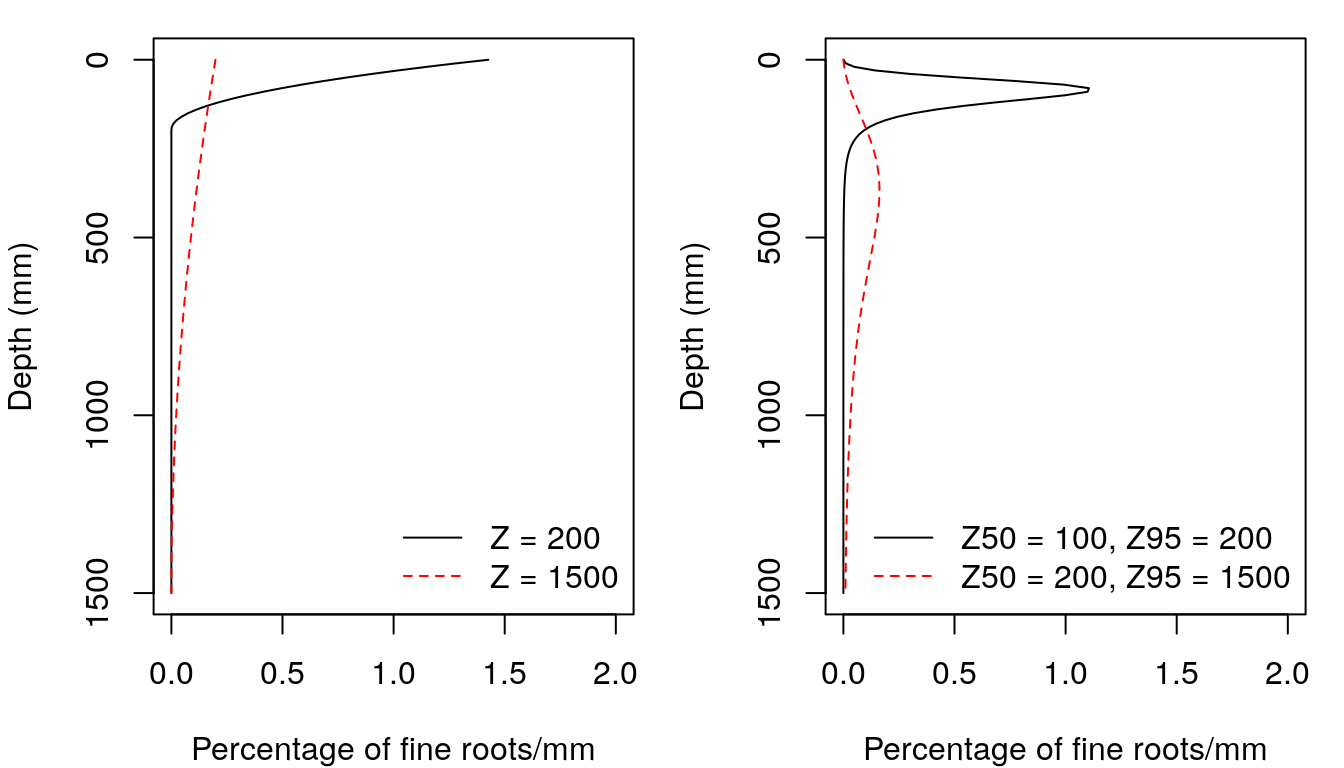
\includegraphics{medfatebook_files/figure-latex/unnamed-chunk-4-1.pdf}
\caption{\label{fig:unnamed-chunk-4}Examples of canopy interception with different S (canopy water storage capacity), E/R (ratio between evaporation and rainfall rates) and p (throughfall coefficient; p = 1 - C)}
\end{figure}

\hypertarget{runoff}{%
\section{Runoff, infiltration and percolation}\label{runoff}}

The water that reaches the soil is the sum of net rainfall (\(Pr_{net}\)), runon (\(Ro\)) and melted snow (\(Sm\)). The amount of water infiltrating into the soil is \(Pr_{net} + Sm + Ro - Ru\), where \(Ru\) is the water lost by surface runoff (see function \texttt{hydrology\_infiltrationAmount}). Surface runoff (in mm), is calculated using the USDA SCS curve number method, as in \citet{Boughton1989}:
\begin{equation}
Ru=\frac{(Pr_{net} + Ro + Sm - 0.2 \cdot V_{soil})^2}{(Pr_{net} + Ro + Sm - 0.8 \cdot V_{soil})}
\end{equation}
where \(V_{soil}\) (in mm) is the overall soil water retention capacity. Following \citet{Granier1999}, part of the water reaching one soil layer percolates quickly through the macropores. The amount of water reaching each layer through macropores is modelled using an extinction function (see function \texttt{hydrology\_infiltrationRepartition}). The remaining water is retained by the micropores refilling the current soil layer. When this soil layer reaches its field capacity the excess of water also percolates to the soil layer below.

\begin{figure}
\centering
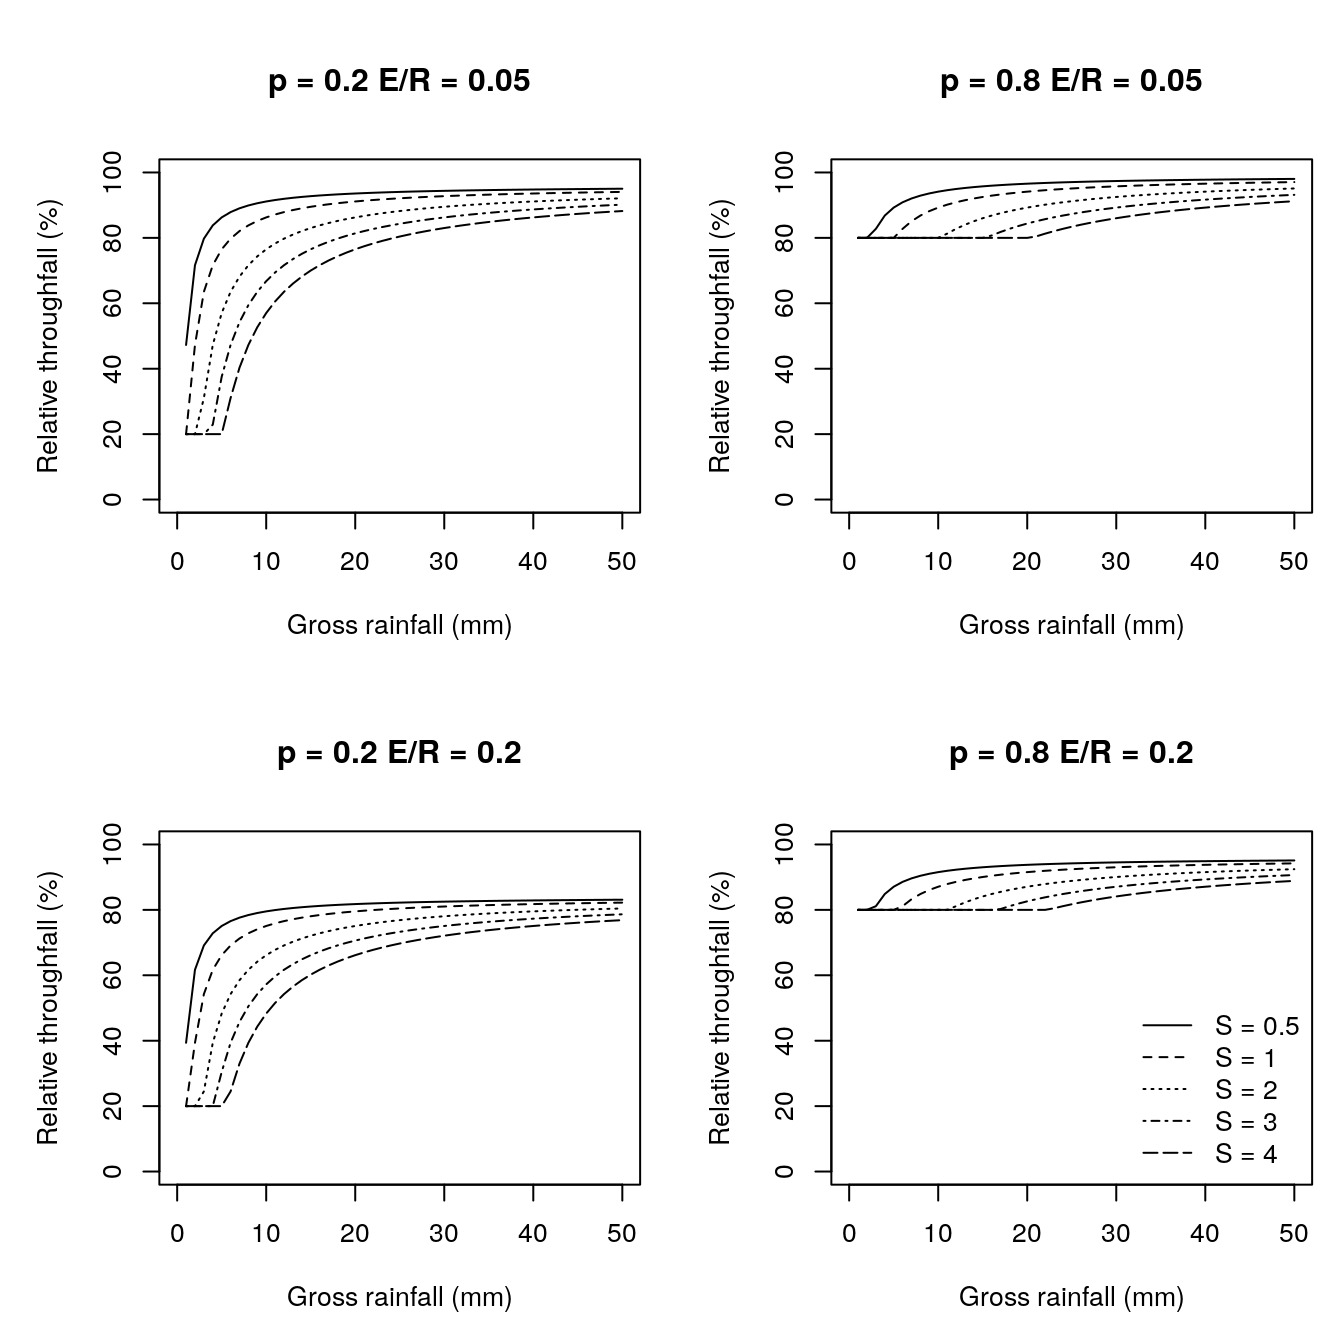
\includegraphics{medfatebook_files/figure-latex/unnamed-chunk-5-1.pdf}
\caption{\label{fig:unnamed-chunk-5}Examples of infiltration/runoff calculation for different values of net rainfall and overall retention capacity, \(V_{soil}\), calculated from different soil depths (topsoil+subsoil) and assuming that soil texture is 15\% clay and 25\% sand. Rock fragment content was 25\% and 40\% for the topsoil and subsoil, respectively.}
\end{figure}

If \texttt{drainage\ =\ TRUE}, the water percolating from the lowest layer is considered deep drainage, \(Dd\), and soil layers are never above field capacity. If \texttt{drainage\ =\ FALSE}, the excess of water in the lowest soil layer is not lost via drainage, so that this layer (and those above) can be filled up to saturation. This additional filling is done starting from below, and when a given layer reaches saturation, the model adds the remaining water to the layer above. If all layers are filled to saturation, the remaining water is assumed to be infiltration excess and is added to the surface runoff.

\hypertarget{bare-soil-evaporation}{%
\section{Bare soil evaporation}\label{bare-soil-evaporation}}

Evaporation from the soil surface is the last component of the soil water balance to be calculated. There is a difference in the way that soil evaporative demand is calculated depending on the transpiration mode. Potential evaporation from the soil (\(PE_{soil}\); in \(mm\cdot day^{-1}\)) is defined as the product between \(PET\) and \(L^{SWR}_{ground}\), the proportion of SWR absorbed by the ground:
\begin{equation}
PE_{soil} =  PET\cdot L^{SWR}_{ground}
\end{equation}

Actual evaporation from the soil surface is modeled as in \citet{Mouillot2001}, who
followed \citet{Ritchie1972}. First, the model determines the time needed to evaporate
the current water deficit (difference between field capacity and current moisture)
in the surface soil layer:
\begin{equation}
t = \left \{ \frac{V_1\cdot(1- W_1)}{\gamma_{soil}} \right \}
\end{equation}
where \(\gamma_{soil}\) is the maximum daily evaporation (mm·day\(^{-1}\)). The
calculated time is used to determine the `supplied' evaporation, \(SE_{soil}\):
\begin{equation}
SE_{soil} = \gamma_{soil} \cdot (\sqrt{t+1}-\sqrt{1})
\end{equation}
The amount of water evaporated from the soil, \(E_{soil}\), is then calculated as
the minimum between supply and demand \citep{Federer1982}, the latter being the product
of PET and the proportion of light that reaches the ground (see function \texttt{hydrology\_soilEvaporationAmount}):

\begin{equation}
E_{soil} = \min(PE_{soil}, SE_{soil})
\end{equation}

Finally, \(E_{soil}\) is distributed along the soil profile according to an exponential decay function with an extinction coefficient \(\kappa_{soil}\) \citep{Mouillot2001}.

\begin{figure}
\centering
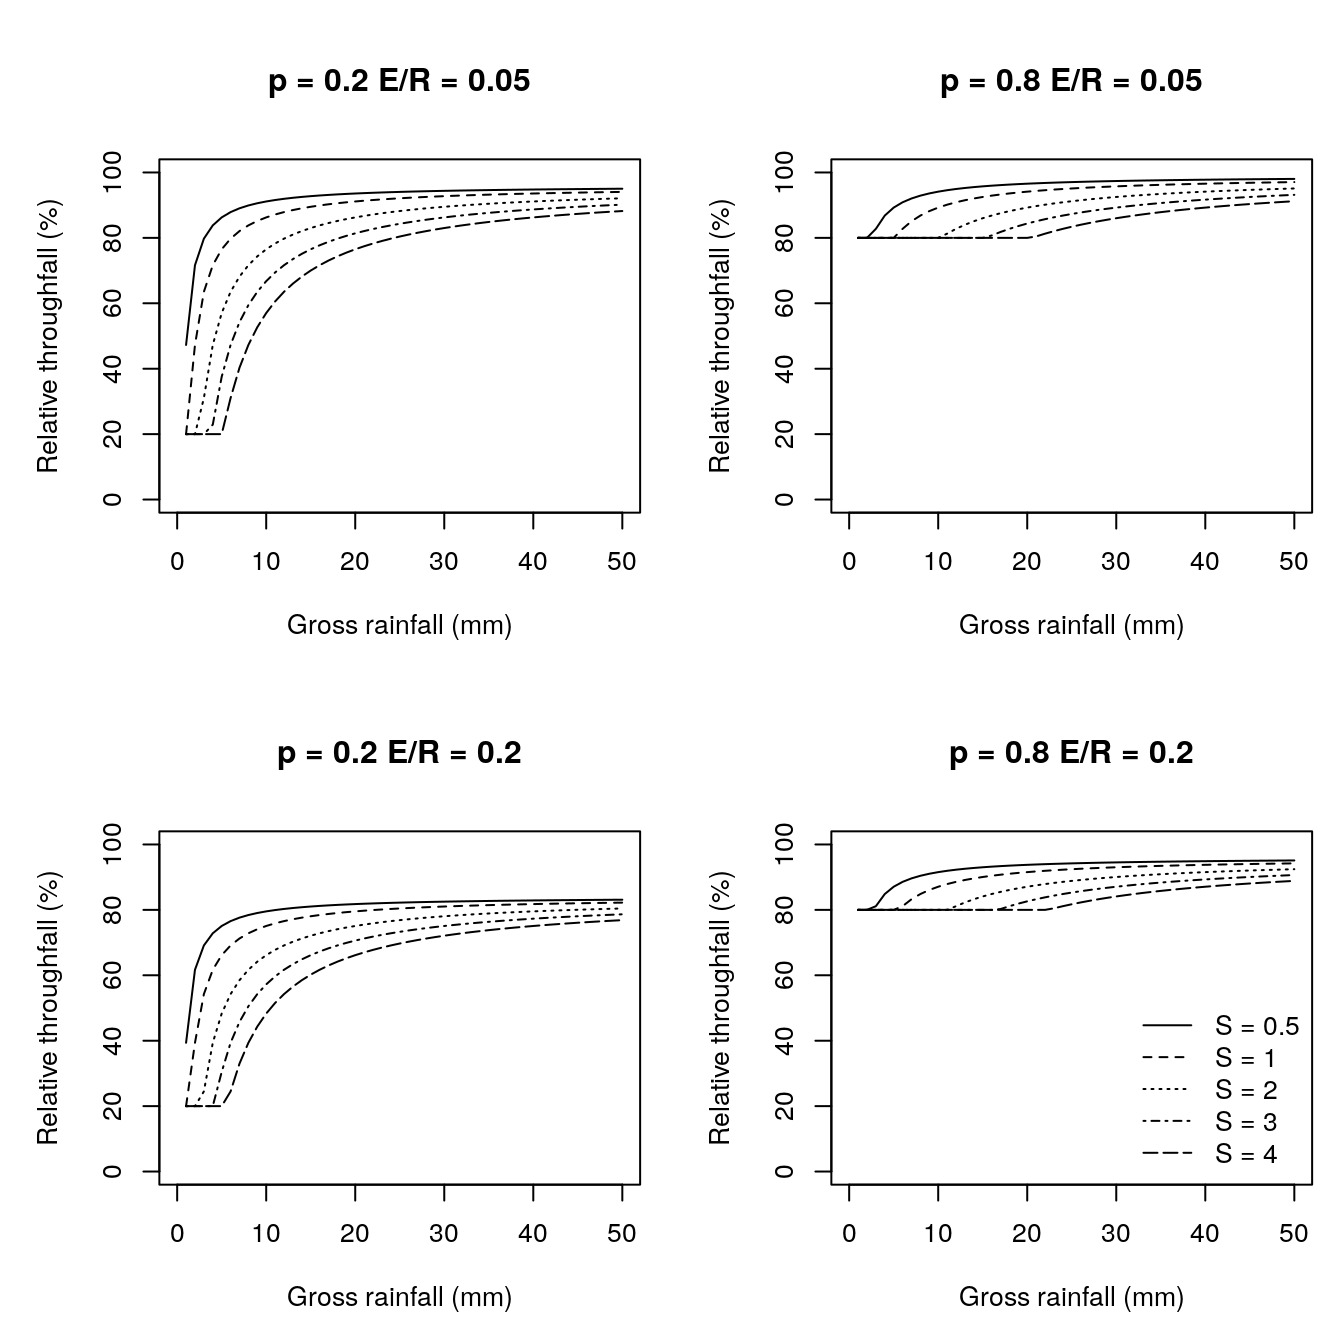
\includegraphics{medfatebook_files/figure-latex/unnamed-chunk-6-1.pdf}
\caption{\label{fig:unnamed-chunk-6}Cumulative bare soil evaporation for different values of maximum evaporation rate and extinction coefficient. Three soil layers (0 -- 30 cm; 30 -- 150 cm; 150 -- 400 cm) are initialized at field capacity (\(V_1 = 50 mm\); \(V_2 = 201 mm\); \(V_3 = 35 mm\)). \(PE_{soil}\) was assumed not to be limiting. When the extinction coefficient is smaller a higher proportion of the evaporated water is removed from the subsoil and less from the topsoil. This causes more water being available to calculate t in the next step.}
\end{figure}

\hypertarget{leaf-phenology-and-light-extinction}{%
\chapter{Leaf phenology and light extinction}\label{leaf-phenology-and-light-extinction}}

\hypertarget{leaf-phenology-and-leaf-fall}{%
\section{Leaf phenology and leaf fall}\label{leaf-phenology-and-leaf-fall}}

Given a base temperature (\(T_{base} = 5^{\circ} \mathrm{C}\)), the growth degree days (\(GDD\)) are zero for all those days where mean temperature \(T_{mean}\) is below \(T_{base}\) and start increasing when temperatures become warmer than this threshold. In other words, the \(GDD\) function accumulates \(\max(0.0, T_{mean} - T_{base})\) for all days previous to the current one. At the end of a year the cummulative value is set again to zero. Plant species can have either evergreen or winter-deciduous phenology. Evergreen plants maintain constant leaf area over the year, whereas in deciduous plants leaf-phenological status is updated daily, represented by \(\phi_i\), the fraction of maximum leaf area. Leaf area index (LAI) values of deciduous plants are adjusted for leaf phenology following \citep{Prentice1993, Sitch2003}:

\begin{equation}
LAI_{i}^{\phi}=LAI^{live}_i\,\cdot\phi_i
\end{equation}

Budburst occurs when daily temperature exceeds \(T_{base}\) and \(\phi_i\) increases
linearly from 0 to 1 as function of the degree days above \(T_{base}\), until a the
value \(S_{GDD,i}\) is reached (i.e.~until \(GDD > S_{GDD,i}\)). In autumn, \(\phi_i\)
drops to 0 when average daily temperature falls again below \(T_{base}\) \citep{Sitch2003}. The drop of \(\phi_i\) causes live expanded leaves to become dead leaves. To avoid a sudden decrease of leaf area, dead leaves are kept in the canopy and they are reduced daily using a negative exponential function of wind speed:
\begin{equation}
LAI^{dead}_i=LAI^{dead}_i\,\cdot e^{- u/10}
\end{equation}
where \(u\) is wind speed in (m·s\(^{-1}\)).

After updating the leaf area of each cohort, the model updates the total leaf area of the stand. To simplify the notation, let us call \(LAI^{all}_{i}\) the sum of dead and live expanded leaves of a cohort \(i\):
\begin{equation}
LAI^{all}_{i} = LAI^{\phi}_{i}+LAI^{dead}_{i}
\end{equation}
If there are \(c\) plant cohorts, the leaf area index of the whole stand, \(LAI_{stand}\)
is then:
\begin{equation}
LAI_{stand} = \sum_{i=1}^c{LAI_{i}^{all}}= \sum_{i=1}^c{LAI^{\phi}_{i}+LAI^{dead}_{i}}
\end{equation}

Although simulations will normally start in winter and \(GDD\) will be zero at the beginning, the user can specify a starting non-zero value for \(GDD\) in the object created by function \texttt{spwbInput()}.

\hypertarget{light-extinction}{%
\section{Light extinction}\label{light-extinction}}

The proportion of photosynthetic active radiation (PAR) decreases with leaf area following thee Beer-Lambert's light extinction equation. To calculate the proportion of PAR available for a given plant cohort one must accumulate the light extinction caused by cohorts whose crown is above that of the target cohort:
\begin{equation}
L^{PAR}_i=e^{-\sum_{h=1}^{c}{k_{PAR,h} \cdot LAI_{h}^{all} \cdot p_{ih}}}
\end{equation}
where \(k_{PAR,h}\) is the PAR extinction coefficient of cohort \(h\). Because plant
cohorts may differ in height only slightly, leaf area is multiplied by \(p_{ih}\),
the proportion of the crown of cohort \(h\) that overtops that of cohort \(i\):
\begin{equation}
p_{ih}=\max(0,\min(1,(H_h-H_i\cdot (1 - CR_i))/(H_h-H_h\cdot (1 - CR_h))))
\end{equation}
where \(CR_i\) and \(CR_h\) are the crown ratio of cohorts \(i\) and \(h\). In other terms,
cohorts whose crown is completely above that of \(i\) reduce the amount of light
available more strongly by than cohorts that are only slightly taller.
\(L^{PAR}_{ground}\), the proportion of PAR that reaches the ground, is calculated as:
\begin{equation}
L^{PAR}_{ground}=e^{-\sum_{i=1}^{c}{k_{PAR,i} \cdot LAI_{i}^{all}}}
\end{equation}

The shortwave radiation (SWR; 400-3000 nm) energy absorbed by each plant cohort
needs to be calculated to determine plant transpiration, and the radiation absorbed
by the soil is needed to calculate soil evaporation. Foliage absorbs a higher
proportion of PAR than SWR; thus, the extinction coefficient is higher for PAR
than for SWR. However, values for the ratio of extinction coefficients are rather
constant. Following Friend et al. \citeyearpar{Friend1997} here it is assumed that the extinction
coefficient for PAR is 1.35 times larger than that for SWR (i.e.
\(k_{SWR,i} = k_{PAR,i}/1.35\)).

To calculate radiation absorption, where the vertical dimension of the plot is
divided into 1 m deep layers, and the SWR absorbed is calculated for each plant
cohort in each layer. Let \(n\) be the number of canopy layers. The fraction of
radiation incident on layer \(j\) that is absorbed in the same layer is:
\begin{equation}
f_j=1 - e^{-\sum_{i=1}^{c}{k_{SWR,i} \cdot LAI_{i,j}^{all}}}
\end{equation}
where \(LAI_{i,j}^{all} = LAI_{i,j}^{\phi}+LAI_{i,j}^{dead}\) is the leaf area
index of cohort \(i\) in layer \(j\). Hence, the fraction transmitted is \((1-f_j)\).
The fraction of radiation incident on layer \(j\) that is absorbed by expanded leaves
of plant cohort \(i\) in that layer (\(f_{ij}\)) is calculated from the relative
contribution of these leaves to the total absorption in the layer:
\begin{equation}
f_{ij} = f_j \cdot \frac{k_{SWR,i}\cdot LAI_{i,j}^{\phi}}{\sum_{h=1}^{c}{k_{SWR,h} \cdot LAI_{h,j}^{all}}}
\end{equation}
The fraction of canopy radiation absorbed by a plant cohort \(i\) across all layers
is found by adding the fraction absorbed in each layer:
\begin{equation}
f_i = \sum_{j=1}^{n}{f_{ij}\cdot \prod_{h>j}^{n}{(1-f_h)}}
\end{equation}
where for each layer the fraction of the radiation incident in the canopy that
reaches the layer is found by multiplying the transmitted fractions across the
layers above it. The proportion of (shortwave) net radiation absorbed by the
ground is simply:
\begin{equation}
L^{SWR}_{ground} = 1 - \sum_{j}^{n}{f_j}
\end{equation}

\hypertarget{transpirationgranier}{%
\chapter{Transpiration and photosynthesis under Granier's model}\label{transpirationgranier}}

\hypertarget{pet-and-maximum-canopy-transpiration}{%
\section{PET and maximum canopy transpiration}\label{pet-and-maximum-canopy-transpiration}}

In this model daily potential evapotranspiration (\(PET\); in mm·day\(^{-1}\); the amount of evaporation that would occur if a sufficient water source was available) is part of the meteorological input and has to be calculated externally. \(PET\) is assumed to represent open water evaporation potential (like in Penman's formula). Maximum canopy transpiration \(Tr_{\max}\) not only depends on \(PET\) but also on the amount of transpirating surface. To estimate \(Tr_{\max}\) we take the approach of \citet{Granier1999}, where \(Tr_{\max}/PET\) is a function of \(LAI_{stand}\) -- the cumulative leaf area of the forest stand --, according to the empirical equation:
\begin{equation}
\frac{Tr_{\max}}{PET}= -0.006\,LAI_{stand}^2+0.134\,LAI_{stand}+0.036
\end{equation}
This equation has already been adopted for Mediterranean biomes (Fyllas and
Troumbis, 2009; Ruffault et al., 2013).

\begin{figure}

{\centering 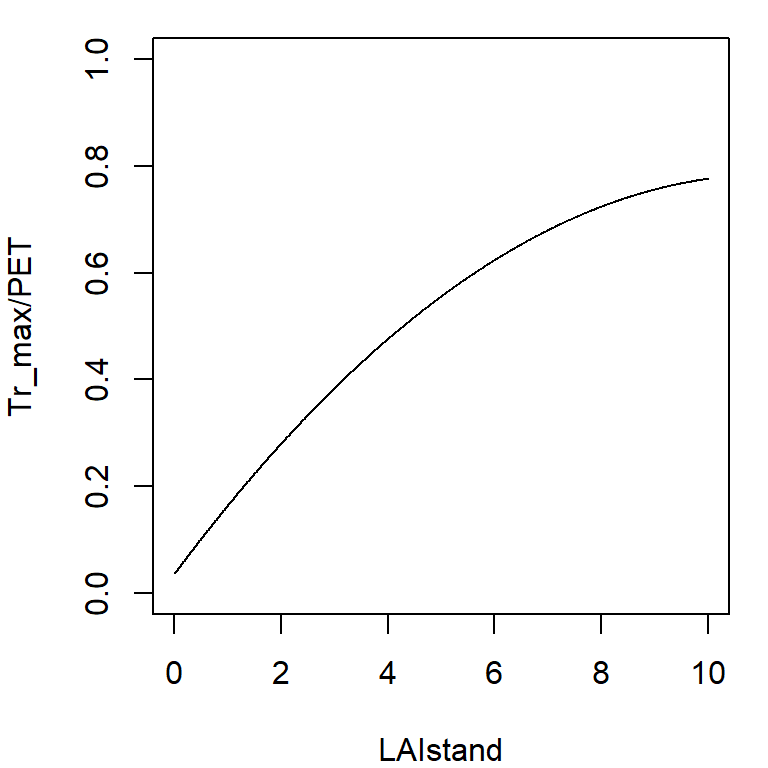
\includegraphics{medfatebook_files/figure-latex/unnamed-chunk-7-1} 

}

\caption{Empirical relationship between $Tr_max/PET$ and $LAI_{stand}$}\label{fig:unnamed-chunk-7}
\end{figure}

The maximum transpiration for a given plant cohort \(i\) is calculated as the
portion of \(Tr_{\max}\) defined by the fraction of total absorbed SWR that is due
to cohort \(i\):
\begin{equation}
Tr_{\max, i} = Tr_{\max} \cdot \frac{f_i}{\sum_{j}{f_j}}
\end{equation}

\hypertarget{actual-plant-transpiration}{%
\section{Actual plant transpiration}\label{actual-plant-transpiration}}

Actual plant transpiration depends on soil moisture and is calculated for each plant cohort and each soil layer separately. \(Tr_{i,s}\) (in mm·day\(^{-1}\)) represents the transpiration made by cohort \(i\) from layer \(s\). Actual plant transpiration from a given layer is regulated by soil moisture and the resistance to water flow through the plant. For each plant cohort \(i\) and soil layer \(s\), the model first estimates the a whole-plant relative water conductance, \(K_{i,s}\), which varies between 0 and 1 depending on \(\Psi_{extract,i}\), the potential at which conductance is 50\% of maximum, and \(\Psi_s\), the water potential in layer \(s\) (see function \texttt{hydraulics\_psi2K()}):
\begin{equation}
K_{i,s}=K_{i}(\Psi_s) = \exp \left \{\ln{(0.5)}\cdot \left[ \frac{\Psi_s}{\Psi_{extract,i}} \right] ^r \right \} 
\end{equation}
where \(r\) is an exponent that modulates the steepness of the decrease in relative
conductance when soil potential becomes negative (by default, \(r = 3\)) and \(\ln(0.5)\)
is used to ensure that \(K_{i}(\Psi_{extract,i}) = 0.5\) (Fig. 4).

\begin{figure}

{\centering 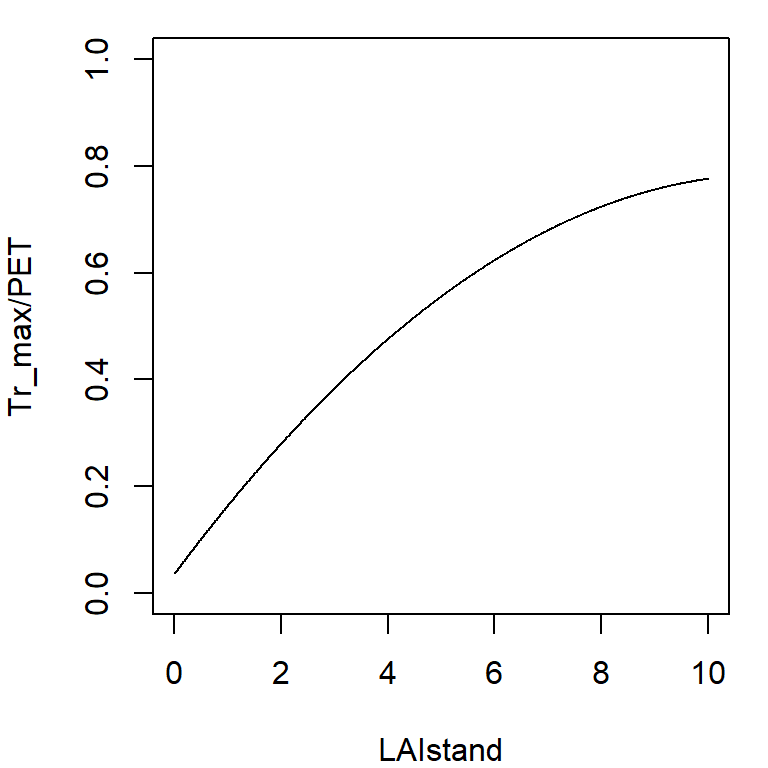
\includegraphics{medfatebook_files/figure-latex/unnamed-chunk-8-1} 

}

\caption{Whole-plant relative water conductance functions for different water potential values ($r = 3$ in all cases).}\label{fig:unnamed-chunk-8}
\end{figure}

Actual transpiration of plant cohort \(i\) from a given soil layer \(s\), \(Tr_{i,s}\),
is defined as the product of (Mouillot et al., 2001): (i) the maximum transpiration
of the plant cohort; (ii) the relative whole-plant conductance, \(K_{i,s}\),
corresponding to the species and water potential in layer \(s\); (iii) the
proportion of plant fine roots in layer \(s\), \(v_{i,s}\):
\begin{equation}
Tr_{i,s} =  Tr_{\max,i} \cdot K_{i,s} \cdot v_{i,s}
\end{equation}
The total amount of water transpired by plants, \(Tr\) (in mm·day\(^{-1}\)), is the sum of
\(Tr_{i,s}\) values over all plant cohorts and soil layers:
\begin{equation}
Tr =\sum_{s}\sum_{i}{Tr_{i,s}}
\end{equation}
Assuming no water limitations (i.e. \(K_{i,s} = 1\)), we have that \(Tr = Tr_{\max}\).
Total stand transpiration will be lower than \(Tr_{\max}\) if soil water potential
in any layer is negative enough to cause a significant reduction in whole-plant
conductance. At the plant level, the transpiration of a given plant cohort will
be lower than that of others if: (1) the cohort is under the shade (it reduces
\(f_i\) and hence \(Tr_{\max,i}\)); (2) the cohort has a lower amount of leaf area
(it reduces \(f_i\) and hence \(Tr_{\max,i}\)); (3) the soil layers exploited by the
cohort have more negative water potentials (it reduces \(K_{i,s}\)).

\hypertarget{plant-photosynthesis}{%
\section{Plant photosynthesis}\label{plant-photosynthesis}}

Because it is useful for growth and forest dynamics, and for compatibility with
the `Sperry' transpiration mode, the `Granier' transpiration mode also calculates
net assimilated carbon. Assuming a constant maximum water use efficiency (WUE),
photosynthesis for a given plant cohort \(i\) (in g C · m\(^{-2}\) · day\(^{-1}\)) is
estimated as a function of transpiration \citep{Mouillot2001}:
\begin{equation}
A_n = \alpha \cdot WUE_{\max} \cdot Tr_i
\end{equation}
where \(Tr_i\) is the transpiration of plant cohort \(i\), \(WUE_{\max}\) is the
maximum water use efficiency of the corresponding species (in g C · mm\(^{-1}\))
and \(\alpha = T_{mean}/20\) is bounded between 0 and 1.

\subsubsection{Plant drought stress and plant water potential}

Similarly to \citet{Mouillot2002}, daily drought stress of a given plant cohort
\(i\), \(DDS_i\), is defined as the complement of relative whole-plant conductance and
is aggregated across soil layers using the proportion of fine roots in each layer
as weights:
\begin{equation}
DDS_i=\phi_i \cdot \sum_{s}{(1-K_{i,s})\cdot v_{i,s}}
\end{equation}
Leaf-phenological status is included to prevent winter deciduous plants from
suffering drought stress during winter. Daily drought stress values can be later
used to define drought stress indices for larger temporal scales, as presented in
the main text.

Granier's transpiration model does not allow estimating a water potential drop
from soil to the leaf. Moreover, in a multilayered soil it is difficult to know
what would be the water potential of the plant. Despite these limitations, a
gross surrogate of (pre-dawn) `leaf water potential' (\(\Psi_{leaf,i}\); in MPa) may be
obtained averaging whole-plant relative conductance values:
\begin{equation}
\Psi_{leaf,i}=K^{-1}(K_i) = K^{-1}\left(\sum_{s}{K_{i,s}\cdot v_{i,s}}\right)
\end{equation}
where \(K_i\) is the average whole-plant relative conductance obtained from the
scalar product of conductances and fine root proportions and \(K^{-1}\) is the inverse of the whole-plant conductance function (see function \texttt{hydraulics\_K2Psi()}).

\hypertarget{irreversible-cavitation-and-hydraulic-disconnection}{%
\section{Irreversible cavitation and hydraulic disconnection}\label{irreversible-cavitation-and-hydraulic-disconnection}}

The water balance model is normally run assuming that although soil drought may
reduce transpiration, embolized xylem conduits are automatically refilled when
soil moisture recovers (in other words, cavitation is reversible). It is possible
to simulate irreversible cavitation by setting \texttt{cavitationRefill\ =\ FALSE} in the control parameters. This option causes the model to keep track of the maximum value of drought stress so far experienced:
\begin{equation}
P_{embolized,i}= \max \{P_{embolized,i}, DDS_i \}
\end{equation}
and then \(K_{i,s}\) cannot be larger than the complement of this maximum drought
stress:
\begin{equation}
K_{i,s} = \min \{K_{i}(\Psi_s), 1.0 - P_{embolized,i} \}
\end{equation}

Another optional behavior consists in allowing the plant to disconnect from the
soil when its potential becomes too negative. This may be advantageous for a
cavitation-sensitive plant that is competing for water with another plant with
higher extraction capacity. Parameter \(K_{rootdisc,i}\) can be used to specify the
minimum relative conductance value that the plant will tolerate without
disconnecting hydraulically from the soil (by default \(K_{rootdisc,i} = 0\)).
If, after possibly accounting for irreversible cavitation, \(K_{i,s}<K_{rootdisc,i}\)
for a given soil layer, then the model assumes that transpiration from this soil
layer is absent. Moreover, \(K_{i,s}\) is assumed equal to \(K_{rootdisc,i}\) for the
sake of determining plant water potential.

\hypertarget{part-advanced-water-balance-modelling}{%
\part{Advanced water balance modelling}\label{part-advanced-water-balance-modelling}}

\hypertarget{advanced-water-balance-model}{%
\chapter{Advanced water balance model}\label{advanced-water-balance-model}}

\hypertarget{design-principles-1}{%
\section{Design principles}\label{design-principles-1}}

The model performs soil water balance and energy balance for the input forest stand and for the period corresponding to input weather data. Soil water balance is calculated on a daily step basis for the input forest stand and for the period corresponding to input weather data. The model considers only the vertical spatial dimension of the stand, and not the horizontal distribution of plants within it. Still, the stand is divided into groups of plants (here referred to as `plant cohorts') of different species, height and leaf area index (\(LAI\)). As hydrological processes, the model includes water interception loss \citep{Gash1995}, plant transpiration and hydraulic redistribution, evaporation from soil \citep{Ritchie1972} and the partition between infiltration and runoff \citep{Boughton1989}. Water exceeding soil water holding capacity is lost via deep drainage. For plant transpiration, the model determines subdaily regulation of leaf water conductance and actual transpiration involving detailed calculations of hydraulics and photosynthesis \citep{Sperry2016}. This level of complexity allows a precise estimation of photosynthesis and hydraulic redistribution of water among soil layers.

Radiation and energy balances are conducted subdaily at two levels: canopy/soil and leaf. One one hand the model keeps track of temperature variation of the air in the canopy (i.e.~canopy energy balance) and in the soil (i.e.~soil energy balance) as the result of energy exchanges between them and with the atmosphere. These energy balance equations are very similar to those of Best et al. \citeyearpar{Best2011} for model JULES. On the other, the model performs the energy balance at the leaf level to determine transpiration \citep{Sperry2016}. At this scale, radiation inputs include shortwave radiation from the atmosphere absorbed by the leaf and absorbed longwave radiation coming from both the atmosphere and the canopy itself. Leaf temperature is determined assuming that the temperature of the air is that of the canopy. After performing stomatal regulation, the model upscales the transpiration flux at the canopy level and the corresponding latent heat is used to complete the calculation of the energy balance at the canopy level. Note that the latent heat fluxes from evaporation from the soil and of intercepted water are not currently included in the energy balance.

\hypertarget{state-variables-1}{%
\section{State variables}\label{state-variables-1}}

The model has the following state variables:
+ Cumulative growth degree days, \(GDD\), are tracked by the model and determine leaf phenological status of winter deciduous species.
+ Daily soil moisture content dynamics on each layer \(s\) are tracked using \(W = \theta(\Psi_s)/ \theta_{fc,s}\), the \textbf{proportion of volumetric soil moisture in relation to field capacity}, where field capacity, \(\theta_{fc,s}\), is assumed to correspond to \(\Psi_{fc} = -0.033\) MPa. Soils are not allowed to contain more water than dictated by their field capacity.
+ The temperature of the canopy and of each soil layer (\(T_c\) and \(T_s\); both in ºC) are tracked for every subdaily step.
+ If irreversible cavitation is activated, the model also tracks \(P_{embolized,i}\), the maximum value of daily drought stress so far experienced.

\hypertarget{water-and-energy-balances}{%
\section{Water and energy balances}\label{water-and-energy-balances}}

\hypertarget{water-balance-1}{%
\subsection{Water balance}\label{water-balance-1}}

Daily variations in soil water content (mm) can be summarized as:

\begin{equation}
\Delta{SWC} = Pr + Sm - In - Ru - Dd - Es -Tr
\end{equation}

where \(Pr\) is precipitation as rainfall, \(Sm\) is water from melting the snow pack (if considered), \(In\) is the interception loss (i.e., water evaporated after being intercepted by the canopy), \(Ru\) is surface runoff, \(Dd\) is deep drainage (i.e.~water percolated to layers beyond soil depth), \(Es\) is evaporation from soil and \(Tr\) is plant transpiration. If snow dynamics are considered, the water balance of the snow pack is defined as:

\begin{equation}
\Delta{S_{snow}} = Ps - Sm
\end{equation}

where \(Ps\) is precipitation as snowfall and \(Sm\) is snow melt.

\hypertarget{energy-balance}{%
\subsection{Energy balance}\label{energy-balance}}

The canopy absorbs shortwave radiation from the atmosphere (\(K_{abs,ca}\)). It also absorbs longwave counterradiation from the atmosphere (\(L_{abs,ca}\)) and longwave radiation emmited from the soil (\(L_{abs,cs}\)). These inputs are counterbalanced by the longwave radiation emmited by the canopy (\(L_{em,c}\)) in both cases. Other energy fluxes considered are convective exchanges between the canopy and atmosphere (\(H_{ca}\)) and between the canopy and the soil (\(H_{cs}\)). Finally, energy is released to the atmosphere through latent heat (\(LE_{c}\)) produced via transpiration (so far, interception and soil evaporation are not included). The instantaneous energy balance equation for the canopy is thus:
\begin{equation}
  C_{c} \cdot \frac{\delta T_{c}}{\delta t} = K_{abs,ca} + (L_{abs,ca} - L_{em,c}) + (L_{abs,cs} - L_{em,c}) - LE_{c} - H_{ca} - H_{cs} 
\end{equation}
where \(C_{c}\) is the canopy thermal capacitance. Like the canopy, the soil absorbs short- and longwave radiation from the atmosphere (\(K_{abs,sa}\) and \(L_{abs,sa}\)). It also absorbs longwave radiation released by the canopy (\(L_{abs,sc} = L_{em,c}\)) and emmits longwave radiation (\(L_{em,s}\)). Note that \(L_{abs,cs} \leq L_{em,s}\) because part of the radiation emmitted by the soil is sent to the atmosphere without being intercepted by the canopy. Finally, it also exchanges convective energy with the canopy (\(H_{cs}\)). The energy balance equation for the soil is:
\begin{equation}
  C_{s} \cdot \frac{\delta T_{s}}{\delta t} = K_{abs,sa} + L_{abs,sa} - L_{em,s} + L_{abs,sc} + H_{cs} 
\end{equation}
where \(C_{s}\) is the soil thermal capacitance.

\hypertarget{process-scheduling-1}{%
\section{Process scheduling}\label{process-scheduling-1}}

Every day the model performs the following actions:

\begin{itemize}
\tightlist
\item
  Update leaf area values according to the phenology of species.
\item
  Increase soil moisture due to precipitation after accounting for canopy interception loss, surface runoff and deep drainage.
\item
  Determine subdaily temperature and direct/diffuse irradiance variations.
\item
  Determine short- and longwave radiation absorved by the canopy and the soil at subdaily steps.
\item
  Determine plant transpiration, photosynthesis and close soil/canopy energy balance at subdaily steps. This involves the following sub-actions:

  \begin{itemize}
  \tightlist
  \item
    Determine longwave radiation emmited by soil and canopy, according to their temperature.
  \item
    Update the water supply function of each plant cohort, according to the hydraulic model and the current soil water potential.
  \item
    Calculate leaf temperature and photosynthesis, for shade and sunlit leaves of each plant cohort, corresponding to each transpiration value of the supply function.
  \item
    Determine stomatal conductance, transpiration and photosynthesis on shade and sunlit leaves of each plant cohort according to a profit maximization strategy.
  \item
    Update soil moisture after scaling transpiration from leaf to canopy level.
  \item
    Complete energy balance of the canopy and the soil (after translating plant transpiration to latent heat and calculating convective heat exchange for both the canopy and the soil).
  \end{itemize}
\item
  Determine drought stress index for each plant cohort.
\item
  Decrease water content due to bare soil evaporation, closing the water balance.
\end{itemize}

\hypertarget{model-input-1}{%
\section{Model input}\label{model-input-1}}

\hypertarget{metereological-input-1}{%
\subsection{Metereological input}\label{metereological-input-1}}

Weather input data must include variables calculated at the \textbf{daily} scale.

\begin{itemize}
\tightlist
\item
  \(T_{min}\) {[}\texttt{MinTemperature}{]}: Minimum temperature (in \(^{\circ} \mathrm{C}\)).
\item
  \(T_{max}\) {[}\texttt{MaxTemperature}{]}: Maximum temperature (in \(^{\circ} \mathrm{C}\)).
\item
  \(RH_{min}\) {[}\texttt{MinRelativeHumidity}{]}: Minimum relative humidity (in percent).
\item
  \(RH_{max}\) {[}\texttt{MaxRelativeHumidity}{]}: Maximum relative humidity (in percent).
\item
  \(P\) {[}\texttt{Precipitation}{]}: Precipitation (in L·m\(^{-2}\) = mm of water).
\item
  \(Rad\) {[}\texttt{Radiation}{]}: Solar radiation after accounting for clouds (in MJ·m\(^{-2}\)).
\item
  \(u\) {[}\texttt{WindSpeed}{]}: Wind speed (in m·s\(^{-1}\)).
\end{itemize}

We recommend meteorological input to be generated using package \textbf{meteoland} \citep{DeCaceres2018}.

\hypertarget{control-parameters-1}{%
\subsection{Control parameters}\label{control-parameters-1}}

Control parameters are a list of parameter values, initialized using function \texttt{defaultControl()}, that the user can modify to change the general behavior of the model. The control values relevant for the advanced water balance model are:

\begin{itemize}
\tightlist
\item
  \texttt{verbose\ {[}=TRUE{]}}: Whether extra console output is desired during simulations.
\item
  \texttt{soilFunctions\ {[}=\ "SX"{]}}: Water retention curve model, either ``SX'' (for Saxton) or ``VG'' (for Van Genuchten).
\item
  \texttt{snowpack\ {[}=\ TRUE{]}}: Whether dynamics of snow pack are included.
\item
  \texttt{drainage\ {[}=\ TRUE{]}}: Whether water exceeding the field capacity of the bottom layer is lost by deep drainage into a non-reachable compartment.
\item
  \texttt{transpirationMode\ {[}=\ "Granier"{]}}: Transpiration model, in this case should be ``Sperry''.
\item
  \texttt{defaultWindSpeed\ {[}=\ 5{]}}: Default value for wind speed (in \(m \cdot s^{-1}\)) when this is missing (only used for leaf fall).
\item
  \texttt{hydraulicCostFunction\ {[}=\ 1{]}}: Variant of the hydraulic cost function used in the stomatal regulation model of \citet{Sperry2016}. Values accepted are 1 (original cost function based on the derivative of supply function), 2 (leaf vulnerability curve).
\item
  \texttt{ndailysteps\ {[}=24{]}}: Number of daily substeps.
\item
  \texttt{thermalCapacityLAI\ {[}=\ 1000000{]}}: Canopy thermal capacitance per LAI unit.
\item
  \texttt{verticalLayerSize\ {[}=\ 100{]}}: The size of vertical layers (in cm) for photosynthesis calculation.
\item
  \texttt{cavitationRefill\ {[}=\ TRUE{]}}: If \texttt{FALSE} the model operates in a irreversible cavitation mode.
\item
  \texttt{taper\ {[}=\ TRUE{]}}: Whether taper of xylem conduits is accounted for when calculating aboveground stem conductance from xylem conductivity.
\item
  \texttt{averageFracRhizosphereResistance\ {[}=\ 0.15{]}}: Fraction to total continuum (stem+root+rhizosphere) resistance that corresponds to rhizosphere (averaged across soil water potential values).
\item
  \texttt{numericParams}: A list with params for numerical approximation routines.
\item
  \texttt{Catm\ {[}=386{]}}: Atmospheric CO2 concentration (in micromol \(CO_2 \cdot mol^{-1}\) = ppm).
\end{itemize}

\hypertarget{species-parameters}{%
\subsection{Species parameters}\label{species-parameters}}

Vegetation functional attributes are normally filled for each cohort by function \texttt{spwbInput()} from species identity. However, different parameters can be specified for different cohort of the same species if desired. Basic functional parameters relate to light extinction, water interception and leaf phenology:

\begin{itemize}
\tightlist
\item
  \(k_{PAR,i}\) {[}\texttt{k}{]}: PAR extinction coefficient.
\item
  \(s_{water, i}\) {[}\texttt{g}{]}: Crown water storage capacity (i.e.~depth of
  water that can be retained by leaves and branches) per LAI unit (in \(mmH_2O·LAI^{-1}\)).
\item
  \(S_{GDD,i}\) {[}\texttt{Sgdd}{]}: Growth degree days corresponding to leave
  budburst (in degrees Celsius).
\end{itemize}

A second set of plant functional parameters are related to plant transpiration and photosynthesis:

\begin{itemize}
\tightlist
\item
  \(g_{wmin,i}\) {[}\texttt{Gwmin}{]}: Minimum leaf water conductance (in \(mol·s^{-1}·m^{-2}\)).
\item
  \(g_{wmax,i}\) {[}\texttt{Gwmax}{]}: Maximum leaf water conductance (in \(mol·s^{-1}·m^{-2}\)).
\item
  \(k_{rhizo,i,s}\) {[}\texttt{VGrhizo\_kmax}{]}: Maximum hydraulic conductance of the rhizosphere for each soil layer.
\item
  \(k_{\max root,i,s}\) {[}\texttt{VCroot\_kmax}{]}: Maximum hydraulic conductance of the root xylem for each soil layer.
\item
  \(c_{root,i}\) and \(d_{root,i}\) {[}\texttt{VCroot\_c} and \texttt{VCroot\_c}{]}: Parameters of the root xylem vulnerability curve.
\item
  \(k_{\max stem,i}\) {[}\texttt{VCstem\_kmax}{]}: Maximum hydraulic conductance of the stem xylem.
\item
  \(c_{stem,i}\) and \(d_{stem,i}\) {[}\texttt{VCstem\_c} and \texttt{VCstem\_c}{]}: Parameters of the stem xylem vulnerability curve.
\item
  \(V298_{max,i}\) {[}\texttt{Vmax298}{]}: Maximum Rubisco carboxylation rate at 25ºC (in \(\mu mol CO_2·s^{-1}·m^{-2}\)).
\item
  \(J298_{max,i}\) {[}\texttt{Jmax298}{]}: Maximum rate of electron transport at 25ºC (in \(\mu mol e ·s^{-1}·m^{-2}\)).\}
\item
  \(P_{rootdisc,i}\) {[}\texttt{pRootDisc}{]}: Relative conductance of roots that leads to hydraulic disconnection from soil.
\item
  \(k_{rhizo,i,s}\) {[}\texttt{VGrhizo\_kmax}{]}: Maximum rhizosphere conductance values for each soil layer.
\item
  \(k_{root,i,s}\) {[}\texttt{VCroot\_kmax}{]}: Maximum root xylem conductance values for each soil layer.
\end{itemize}

\hypertarget{model-output-1}{%
\section{Model output}\label{model-output-1}}

Function \texttt{spwb} with \texttt{transpirationMode\ =\ "Sperry"} returns a list object whose elements are data tables. Each table has dates as rows and has different output variables:

\begin{itemize}
\tightlist
\item
  \texttt{WaterBalance}: Components of the climatic and soil daily water balance (i.e.~net precipitation, infiltration, runoff, plant transpiration\ldots{}).
\item
  \texttt{Soil}: Daily variation of soil variables (volume, moisture relative to field capacity, water potential) for soil layers.
\item
  \texttt{EnergyBalance}: Components of the atmosphere-canopy-soil energy balance, including latent heat, convective heat, conduction heat and radiation exchanges.
\item
  \texttt{PlantLAI}: Daily leaf area index for each plant cohort.
\item
  \texttt{PlantTranspiration}: Daily transpiration (in mm) for each plant cohort.
\item
  \texttt{PlantPhotosynthesis}: Daily net photosynthesis (in g C·m-2) for each plant cohort.
\item
  \texttt{PlantPsi}: Daily water potential of each plant (in MPa).
\item
  \texttt{PlantStress}: Daily stress level suffered by each plant cohort (relative whole-plant conductance).
\end{itemize}

\hypertarget{subdaily-temperature-and-light-variations}{%
\chapter{Subdaily temperature and light variations}\label{subdaily-temperature-and-light-variations}}

\hypertarget{air-temperature}{%
\section{Air temperature}\label{air-temperature}}

Diurnal above-canopy air temperature (\(T_a\)) variations are modeled assuming a sinusoidal pattern with \(T_a = T_{\min}\) at sunrise and \(T_a = (T_{\min}+T_{\max})/2\) at sunset. Air temperature varies linearly between sunset and sunrise \citep{McMurtrie1990}.

\hypertarget{diffuse-and-direct-radiation}{%
\section{Diffuse and direct radiation}\label{diffuse-and-direct-radiation}}

Daily global radiation (in MJ·m\(^{-2}\)) is assumed to include both direct and diffuse shortwave radiation (SWR). Using latitude information and whether is a rainy day, this quantity is partitioned into instantaneous direct and diffuse SWR and PAR for different daily substeps. Values of instantaneous direct and diffuse SWR and PAR above the canopy (i.e. \(I_{beam}\) and \(I_{dif}\)) are calculated using the methods described in \citet{Spitters1986}, which involve comparing daily global radiation with daily potential radiation.

\hypertarget{longwave-radiation}{%
\section{Longwave radiation}\label{longwave-radiation}}

Longwave radiation (LWR) coming from the atmosphere is calculated following \citet{Campbell1998}:
\begin{equation}
L_{a} = \epsilon_{a} \cdot \sigma \cdot (T_{a} + 273.16)^{4.0}
\end{equation}
where \(T_{a}\) is air temperature, \(\sigma = 5.67 \cdot 10^{-8.0}\) W·K\(^{-4}\)·m\(^{-2}\) is the Stephan-Boltzmann constant and \(\epsilon_{a}\) is the emmissivity of the atmosphere, calculated using:
\begin{eqnarray}
\epsilon_{a} &=& (1 - 0.84 \cdot c) \cdot \epsilon_{ac} + 0.84 \cdot c \\
\epsilon_{ac} &=& 1.72 \cdot \left(\frac{vp_{day}}{T_{a} + 273.16} \right)^{1/7}
\end{eqnarray}
where \(vp_{day}\) is the average daily vapor pressure (in kPa) and \(c\) is the proportion of clouds.

\hypertarget{radiation-balance}{%
\chapter{Radiation balance}\label{radiation-balance}}

The following subsection detail the calculation of radiation components of the energy balance equations.

\hypertarget{shortwave-radiation-absorbed-by-the-canopy}{%
\section{Shortwave radiation absorbed by the canopy}\label{shortwave-radiation-absorbed-by-the-canopy}}

The canopy is divided into vertical layers (whose size is determined by the control parameter \texttt{verticalLayerSize}), and the expanded and dead leaf area index of each cohort within each layer is determined. Let \(n\) be the number of canopy layers. And let \(LAI_{i,j}^{all} = LAI_{i,j}^{\phi}+LAI_{i,j}^{dead}\) be the leaf area index of cohort \(i\) in layer \(j\). Furthermore, it is generally accepted that sunlit and shade leaves need to be treated separately \citep{DePury1997}. This separation is necessary because photosynthesis of shade leaves has an essentially linear response to irradiance, while photosynthesis of leaves in sunflecks is often light saturated and independent of irradiance.

The average irradiance reaching the top of each canopy layer \(j\) is calculated separately for direct beam and diffuse radiation:
\begin{eqnarray}
I_{beam,j} &=& (1 - \gamma) \cdot I_{beam} \cdot \exp\left[ \sum_{h=j+1}^{n}{\sum_{i}^{c}{-k_{b,i}\cdot \alpha_i^{0.5}\cdot LAI^{all}_{i,h}}}\right]\\
I_{dif,j} &=& (1 - \gamma) \cdot I_{dif} \cdot \exp\left[ \sum_{h=j+1}^{n}{\sum_{i}^{c}{-k_{d,i}\cdot \alpha_i^{0.5}\cdot LAI^{all}_{i,h}}}\right]
\end{eqnarray}
where \(I_{beam}\) and \(I_{dif}\) are the direct and diffuse irrradiance at the top of the canopy, \(\gamma\) is the leaf reflectance (\(\gamma_{PAR} = 0.04\), \(\gamma_{SWR} = 0.05\)), \(k_{b,i}\) is the extinction coefficient of cohort \(i\) for direct light (\(k_{b,i} = 0.8\)), \(k_{d,i}\) is the extinction coefficient of cohort \(i\) for diffuse light (i.e. \(k_{PAR}\) or \(k_{SWR}\)) and \(\alpha_i\) is the absorbance coefficient (\(\alpha_{i,PAR} = 0.9\), \(\alpha_{i,SWR} = 0.7\)).

The proportion of sunlit leaves, i.e.~leaves in a canopy layer that the direct light beams (sunflecks) reach is:
\begin{equation}
f_{SL, j}  = \exp\left( \sum_{k>j}^{n}{\sum_{i}^{c}{-k_{b,i} \cdot LAI^{all}_{i,k}}}\right) \cdot \exp\left( \sum_{i}^{c}{-k_{b,i} \cdot 0.5\cdot LAI^{all}_{i,j}}\right)
\end{equation}
As an example we will consider a canopy of one species of LAI = 2, divided into ten layers with constant leaf density.

This canopy definition leads to a percentage of the above-canopy irradiance reaching each layer \citep{Anten2016}. Extinction of direct radiation also defines the proportion of leaves of each layer that are affected by sunflecks (i.e.~the proportion of sunlit leaves).

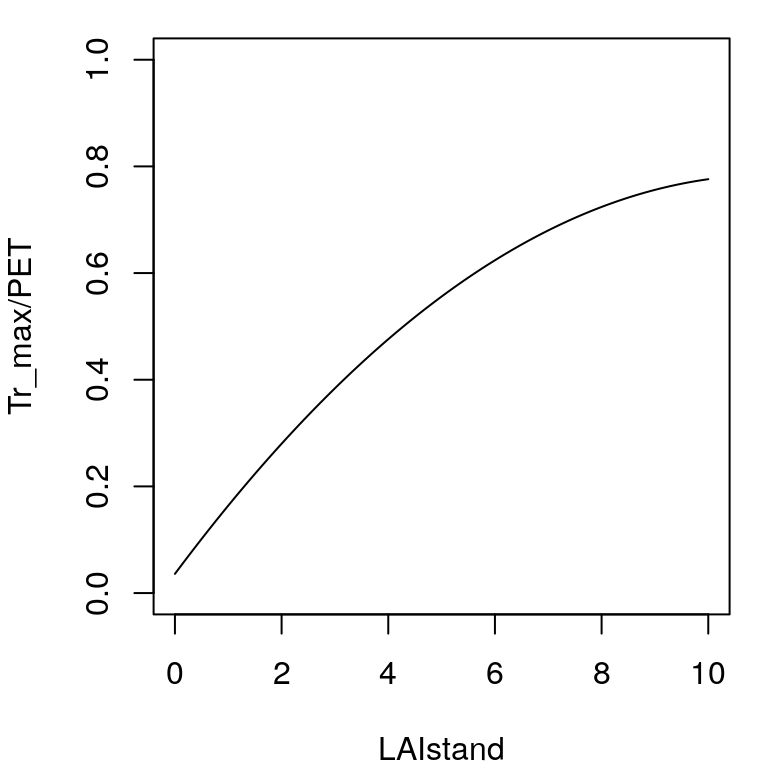
\includegraphics{medfatebook_files/figure-latex/unnamed-chunk-10-1.pdf}

The amount of absorved diffuse radiation per leaf area unit of cohort \(i\) within a given canopy layer \(j\) is calculated as:
\begin{equation}
I_{dif,i,j} = I_{dif,j} \cdot k_{d,i} \cdot \alpha_i^{0.5} \exp\left[ \sum_{h}^{c}{-k_{d,h}\cdot \alpha_h^{0.5}\cdot 0.5\cdot LAI^{all}_{h,j}}\right]
\end{equation}

The amount of absorved scattered beam radiation per leaf area unit of cohort \(i\) within a given canopy layer \(j\) is calculated as:
\begin{equation}
% \begin{split}
I_{sca,i,j} = I_{b,j} \cdot k_{b,i} \left( \alpha_i^{0.5}\cdot \exp \left( \sum_{h}^{c}{-k_{b,h}\cdot \alpha_h\cdot 0.5\cdot LAI^{all}_{h,i}}\right) 
-\frac{\alpha_i}{(1-\gamma)}\cdot \exp\left( \sum_{h}^{c}{-k_{b,h}\cdot 0.5\cdot LAI^{all}_{h,i}}\right) \right)
% \end{split}
\end{equation}

Finally, the direct radiation absorbed by a unit of sunlit leaf area of cohort \(i\) in a canopy layer \(j\) does not depend on the position of the canopy layer and is:
\begin{equation}
I_{dir,i,j} = I_{beam} \cdot \alpha_i \cdot 0.5/\sin{\beta}
\end{equation}
where \(\beta\) is the solar elevation angle, which changes throughout the day. The amount of light absorbed by shaded/sunlit foliage of cohort \(i\) in layer \(j\) per leaf area unit (\(I_{SH,i,j}\) and \(I_{SL,i,j}\), respectively) is:
\begin{eqnarray}
I_{SH,i,j} &=& I_{dif,i,j} + I_{sca,i,j} \\
I_{SL,i,j} &=& I_{dif,i,j} + I_{sca,i,j} + I_{dir,i,j}
\end{eqnarray}
The total amount of light absorbed by shaded/sunlit foliage of cohort \(i\) per ground area unit is found by taking into account the proportion of sunlit foliage:
\begin{eqnarray}
\Phi_{SH,i,j} &=& I_{SH,i,j}\cdot (1 - f_{SL,j}) \cdot LAI^{\phi}_{i,j}\\
\Phi_{SL,i,j} &=& I_{SL,i,j}\cdot f_{SL,j} \cdot LAI^{\phi}_{i,j}
\end{eqnarray}

\hypertarget{shortwave-radiation-absorbed-by-the-soil}{%
\section{Shortwave radiation absorbed by the soil}\label{shortwave-radiation-absorbed-by-the-soil}}

The instantaneous shortwave radiation reaching the soil is calculated separately for direct beam and diffuse radiation:
\begin{eqnarray}
K_{beam, soil} &=&  K_{beam} \cdot \exp\left[ \sum_{h=j+1}^{n}{\sum_{i}^{c}{-k_{b,i}\cdot \alpha_i^{0.5} \cdot LAI^{all}_{i,h}}}\right]\\
K_{dif, soil} &=& K_{dif} \cdot \exp\left[ \sum_{h=j+1}^{n}{\sum_{i}^{c}{-k_{d,i}\cdot LAI^{all}_{i,h}}}\right]
\end{eqnarray}
where \(K_{beam}\) and \(K_{dif}\) are the direct and diffuse irrradiance at the top of the canopy, \(k_{b,i}\) is the extinction coefficient of cohort \(i\) for direct light (\(k_{b,i} = 0.8\)) and \(k_{d,i}\) is the extinction coefficient of cohort \(i\) for diffuse SWR. From these, the SWR absorbed by the soil is found by:
\begin{equation}
K_{abs,sa} = (1 - \gamma_{SWR, soil})\cdot (K_{beam, soil} + K_{dif, soil})
\end{equation}
where \(\gamma_{SWR, soil} = 0.10\) is the SWR reflectance (10\% albedo) of the soil. LWR is treated in the same way as diffuse SWR. The instantaneous LWR reaching the soil is:
\begin{equation}
L_{abs,sa} = (1 - \gamma_{LWR, soil})\cdot L_{a} \cdot \exp\left[ \sum_{h=j+1}^{n}{\sum_{i}^{c}{-k_{LWR}\cdot LAI^{all}_{i,h}}}\right]
\end{equation}
where \(L_a\) is the atmosphere longwave irradiance, \(k_{LWR} = 0.8\) is the extinction coefficient for LWR and \(\gamma_{LWR, soil} = 0.05\) is LWR soil reflectance (5\% albedo) of the soil.

\hypertarget{longwave-soil-canopy-radiation-exchange}{%
\section{Longwave soil-canopy radiation exchange}\label{longwave-soil-canopy-radiation-exchange}}

Longwave radiation (LWR) emmited by a surface at the canopy temperature \(T_{can}\) would be:
\begin{equation}
L_{em} = 0.95 \cdot \sigma \cdot (T_{can} + 273.16)^{4.0}
\end{equation}
where \(0.95\) is emissivity and \(\sigma = 5.67 \cdot 10^{-8.0} Wm^{-2}\) is the Stephan-Boltzmann constant. However, the canopy may only partially cover the soil surface, so the value must be reduced by the proportion of the canopy layer actually exchanging energy. We take this as the proportion between atmospheric and absorbed LWR:
\begin{eqnarray}
p_{exch} &=& \frac{L_{abs,ca}}{L_a} \\
L_{em, c} &=& p_{exch} \cdot L_{em}
\end{eqnarray}
\(L_{em, c}\) is discounted twice from the canopy energy balance: as losses to the atmosphere and losses to the soil.

LWR emmited by the soil is calculated from the temperature of the first soil layer:
\begin{equation}
L_{em, s} = 0.95 \cdot \sigma \cdot (T_{soil} + 273.16)^{4.0}
\end{equation}

Again, the canopy only absorbs part of this radiation, the remaining going to the atmosphere:

\begin{equation}
L_{abs, cs} = p_{exch} \cdot L_{em,s}
\end{equation}

\hypertarget{canopy-and-soil-energy-balances}{%
\chapter{Canopy and soil energy balances}\label{canopy-and-soil-energy-balances}}

\hypertarget{convective-energy}{%
\section{Convective energy}\label{convective-energy}}

Convective energy fluxes between atmosphere and the canopy (\(H_{ca}\)) and between the canopy and the soil (\(H_{cs}\)) are determined as follows:
\begin{eqnarray}
H_{ca} &=& \frac{\rho_{a} \cdot c_p}{r_{ca}}\cdot (T_{can} - T_a) \\
H_{cs} &=& \frac{\rho_{c} \cdot c_p}{r_{cs}}\cdot (T_{can} - T_{soil})
\end{eqnarray}
where \(\rho_{a}\) and \(\rho_{c}\) are the air density above-canopy and inside-canopy, respectively, \(c_{p}\) = 1013.86 \(J·kg^{-1}·C^{-1}\) is the specific heat capacity of the air. \(r_{ca}\) and \(r_{cs}\) are the atmosphere-canopy and canopy-soil aerodynamic resistances (in \(s·m^{-1}\)). These, in turn, are calculated using canopy height, total LAI and above-canopy and below-canopy wind speeds.

\hypertarget{latent-heat}{%
\section{Latent heat}\label{latent-heat}}

As mentioned above, the model only considers latent heat exchanged from plant transpiration, neglecting energy fluxes corresponding to evaporation from the soil and evaporation of rain intercepted by the canopy. After determining stomatal regulation and transpiration for each plant cohort, latent heat of transpiration is simply calculated as:
\begin{equation}
LE_{c} = \lambda_{T_{can}} \sum_{i}{E_i}
\end{equation}
where \(\lambda_{T_{can}}\) is the latent heat of vaporization at temperature \(T_{can}\) (in J·kg\(^{-1}\)) and \(E_i\) is the instanteous transpiration flux calculated for cohort \(i\).

\hypertarget{canopy-capacitance-and-temperature-changes}{%
\section{Canopy capacitance and temperature changes}\label{canopy-capacitance-and-temperature-changes}}

TO BE DONE

\hypertarget{soil-temperature-changes}{%
\section{Soil temperature changes}\label{soil-temperature-changes}}

Instantaneous soil temperature changes on each soil layer depend on the balance between incoming and outcoming energies (\(G_k\) and \(G_{k-1}\)):
\begin{equation}
\frac{\delta T_{soil,k}}{\delta t} = \frac{G_k - G_{k-1}}{C_{soil,k} \cdot \Delta z_k}
\end{equation}
where \(\Delta z_k\) is the soil width of layer \(k\) and \(C_{soil,k}\) is the thermal capacity of layer \(k\), depending on soil moisture and texture (see function \texttt{soil\_thermalcapacity}).

Energy inflow to the first layer (i.e. \(G_0\)) is the result of the soil energy balance explained above, while energy transfers between layers (i.e. \(G_k\)) depend on the soil temperature gradient:
\begin{eqnarray}
G_0 &=& K_{abs,sa} + L_{abs,sa} - L_{em,s} + L_{abs,sc} + H_{cs}\\
G_k &=& \lambda_{soil,k} \cdot \frac{\delta T_{soil,k}}{\delta z}
\end{eqnarray}
where \(\lambda_{soil,k}\) is the thermal conductivity of layer \(k\), depending on soil moisture and texture (see function \texttt{soil\_thermalconductivity}). The gradient in the bottom layer is calculated assuming a temperature of the earth (at 10 m) of 15.5 Celsius.

\hypertarget{bare-soil-evaporation-1}{%
\section{Bare soil evaporation}\label{bare-soil-evaporation-1}}

Evaporation from the soil surface is the last component of the soil water balance to be calculated. Soil evaporative demand, i.e.~potential evaporation from the soil (\(PE_{soil}\); in \(mm\cdot day^{-1}\)), is calculated using the Penman-Monteith combination equation:
\begin{equation}
PE_{soil} = \frac{1}{\lambda} \cdot \frac{\Delta \cdot R_{n,soil} + D \cdot (\rho \cdot C_p/r_a)}{\Delta + \gamma \cdot (1 + r_{soil}/r_a)}
\end{equation}
where \(D\) is the vapour pressure deficit (in kPa), \(\Delta\) is the slope of the saturated vapor pressure (in \(Pa \cdot K^{-1}\)), \(\gamma\) is the psychrometer constant (in \(kPa\cdot K^{-1}\)), \(\lambda\) is the latent heat vaporization of water (in \(MJ\cdot kg^{-1}\)) and \(C_p\) is the specific heat of air (in \(MJ\cdot kg^{-1}\cdot K^{-1}\)). \(r_{soil}\) is the resistance of the soil surface, set to a constant value (\(r_{soil} = 200\) \(s\cdot m^{-1}\)). For simplicity, aerodynamic resistance (\(r_a\)) in the soil is currently set to \(r_a = 208.0/u\) where \(u\) is the input wind speed.

\hypertarget{plant-hydraulics}{%
\chapter{Plant hydraulics}\label{plant-hydraulics}}

The supply-loss theory of plant hydraulics, presented by \citet{Sperry2016} and used in \citet{Sperry2016}, uses the physics of flow through soil and xylem to quantify how steady-state canopy water supply declines with drought and ceases by hydraulic failure. The theory builds on the hydraulic model of \citet{Sperry1998} and can be applied to different segmentations of the soil-plant continuum. In our case we considered a network of \((N \times 2 + S + 1)\) resistance elements, with soil being represented in \(N\) different layers and \(S\) different stem segments. For each soil layer there is a rhizosphere element in series with a root xylem element. The \(N\) soil layers are in parallel up to the root crown. From there there are \(S\) stem xylem segments and a final leaf segment, all in series. Althougth the model implements this network representation of the soil-plant continuum, simpler one-element, two-element and three-element representations will be used in this document to facilitate understanding.

\hypertarget{vulnerability-curves}{%
\section{Vulnerability curves}\label{vulnerability-curves}}

Each continuum element has a vulnerability curve that starts at maximum hydraulic conductance (\(k_{max}\), flow rate per pressure drop) and monotonically declines as water pressure (\(\Psi\)) becomes more negative. Vulnerability curves form the basis of hydraulic calculations.

\hypertarget{xylem-vulnerability-curves}{%
\subsection{Xylem vulnerability curves}\label{xylem-vulnerability-curves}}

Xylem tissues are assigned a two-parameter Weibull function as the vulnerability curve \(k(\Psi)\):
\begin{equation}
k(\Psi) = k_{max}\cdot e^{-((\Psi/d)^c)}
\label{eq:xylemvulnerability}
\end{equation}
where \(k_{max}\) is the maximum hydraulic conductance (defined as flow per leaf surface unit and per pressure drop), and \(c\) and \(d\) are species-specific and tissue-specific parameters. Note that parameter \(d\) is the water potential (in MPa) at which \(k(\Psi)/k_{max} = e^{-1} = 0.367\). Parameter \(c\) controls the shape of the vulnerability curve (`exponential' shape with no threshold has \(c \leq 1\), sigmoidal threshold has \(c > 1\)).

For example, we define the following parameter values for a stem xylem (\(k_{s,max}\) and parameters \(c_s\) and \(d_s\) of the vulnerability curve):

\begin{Shaded}
\begin{Highlighting}[]
\NormalTok{kstemmax =}\StringTok{ }\FloatTok{5.0} \CommentTok{# mmol·m-2·s-1·MPa-1}
\NormalTok{stemc =}\StringTok{ }\DecValTok{3} 
\NormalTok{stemd =}\StringTok{ }\FloatTok{-3.0} \CommentTok{# MPa}
\end{Highlighting}
\end{Shaded}

For root xylem (\(k_{r,max}\)), we may assume a higher conductance (i.e.~higher efficiency) but also higher vulnerability to cavitation (defined by parameters \(c_r\) and \(d_r\)):

\begin{Shaded}
\begin{Highlighting}[]
\NormalTok{krootmax =}\StringTok{ }\FloatTok{6.6} \CommentTok{# mmol·m-2·s-1·MPa-1}
\NormalTok{rootc =}\StringTok{ }\DecValTok{2}
\NormalTok{rootd =}\StringTok{ }\FloatTok{-2.5} \CommentTok{#MPa}
\end{Highlighting}
\end{Shaded}

The concept of vulnerability curve can be used to specify the relationship between pressure and conductance in any portion of the flow path. Leaf vulnerability curve \(k_l(\Psi)\) can be modelled using the same equation as for xylem:
\begin{equation}
k_l(\Psi) = k_{l,max}\cdot e^{-((\Psi/d_l)^{c_l})}
\label{eq:leafvulnerability}
\end{equation}
where \(k_{l,max}\) is the leaf maximum hydraulic conductance. Values defined below specify higher conductance for leaves but also slightly higher vulnerability:

\begin{Shaded}
\begin{Highlighting}[]
\NormalTok{kleafmax =}\StringTok{ }\DecValTok{10}
\NormalTok{leafc =}\StringTok{ }\DecValTok{2}
\NormalTok{leafd =}\StringTok{ }\DecValTok{-2}
\end{Highlighting}
\end{Shaded}

With these parameter values, the vulnerability curves for root, stem and leaf are (see \texttt{hydraulics\_xylemConductance()}):

\begin{center}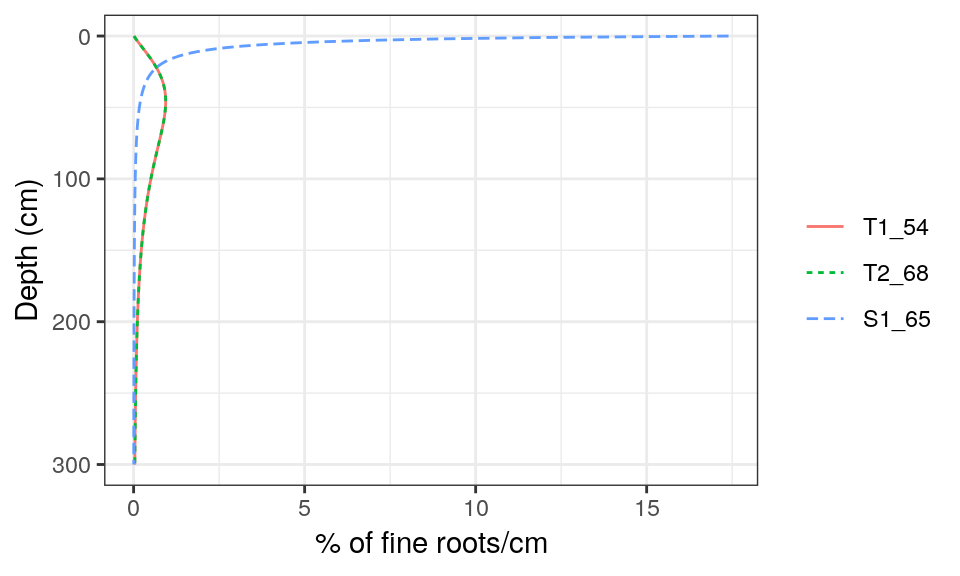
\includegraphics{medfatebook_files/figure-latex/unnamed-chunk-16-1} \end{center}

The dotted line between 0 and \(\Psi_{cav} = -2.5\) MPa indicates the modification of the stem xylem vulnerability curve when cavitation has occurred (i.e., previous embolism limits a the maximum conductance value), as indicated in \citet{Sperry2016}. The corresponding proportion of conductance loss can be found using the stem vulnerability curve:
\begin{equation}
PLC(\Psi_{cav}) = 1.0 - \frac{k_s(\Psi_{cav})}{k_{s,max}} = 1.0 - e^{-((\Psi/{d_s})^{c_s})}
\end{equation}

\begin{Shaded}
\begin{Highlighting}[]
\FloatTok{1.0} \OperatorTok{-}\StringTok{ }\KeywordTok{exp}\NormalTok{(}\OperatorTok{-}\NormalTok{(}\OperatorTok{-}\FloatTok{2.5}\OperatorTok{/}\NormalTok{stemd)}\OperatorTok{^}\NormalTok{stemc)}
\end{Highlighting}
\end{Shaded}

\begin{verbatim}
## [1] 0.4393754
\end{verbatim}

Although root xylem are more vulnerable to the formation of emboli for a given potential, it is generally accepted that the less negative potentials of root xylem compared to the stem lead to cavitation occurring more often in the stem. The constrain created by cavitation has an effect on the calculation of the flow rates and derived quantities (see below).

\hypertarget{rhizosphere-vulnerability-curve}{%
\subsection{Rhizosphere vulnerability curve}\label{rhizosphere-vulnerability-curve}}

The rhizosphere conductance function \(k_{rh}(\Psi)\) is modeled as a van Genuchten function \citep{Genuchten1980}:
\begin{eqnarray}
k_{rh}(\Psi) &=& k_{rh,max} \cdot v^{(n-1)/(2\cdot n)} \cdot ((1-v)^{(n-1)/n}-1)^2 \\
v &=& [(\alpha \Psi)^{n}+1]^{-1}
\label{eq:rhizovulnerability}
\end{eqnarray}
where \(k_{rh,max}\) is the maximum rhizosphere conductance, and \(n\) and \(\alpha\) are texture-specific parameters \citep{Leij1996, Carsel1988}. These are automatically set by function \texttt{soil()} when initializing soil objects (see parameters \texttt{VG\_alpha} and \texttt{VG\_n} in the output of \texttt{soil()}), but we can use function \texttt{soil\_vanGenuchtenParamsCarsel()} to derive them from texture types:

\begin{Shaded}
\begin{Highlighting}[]
\NormalTok{textures =}\StringTok{ }\KeywordTok{c}\NormalTok{(}\StringTok{"Sandy loam"}\NormalTok{,}\StringTok{"Silt loam"}\NormalTok{, }\StringTok{"Clay"}\NormalTok{)}
\CommentTok{#Textural parameters}
\CommentTok{#Sandy clay loam }
\NormalTok{p1 =}\StringTok{ }\KeywordTok{soil_vanGenuchtenParamsCarsel}\NormalTok{(textures[}\DecValTok{1}\NormalTok{])}
\NormalTok{p1}
\end{Highlighting}
\end{Shaded}

\begin{verbatim}
##     alpha         n theta_res theta_sat 
##   764.983     1.890     0.065     0.410
\end{verbatim}

\begin{Shaded}
\begin{Highlighting}[]
\NormalTok{alpha1 =}\StringTok{ }\NormalTok{p1[}\DecValTok{1}\NormalTok{]  }
\NormalTok{n1 =}\StringTok{ }\NormalTok{p1[}\DecValTok{2}\NormalTok{]}
\CommentTok{#Silt loam}
\NormalTok{p2 =}\StringTok{ }\KeywordTok{soil_vanGenuchtenParamsCarsel}\NormalTok{(textures[}\DecValTok{2}\NormalTok{])}
\NormalTok{p2}
\end{Highlighting}
\end{Shaded}

\begin{verbatim}
##     alpha         n theta_res theta_sat 
##  203.9955    1.4100    0.0670    0.4500
\end{verbatim}

\begin{Shaded}
\begin{Highlighting}[]
\NormalTok{alpha2 =}\StringTok{  }\NormalTok{p2[}\DecValTok{1}\NormalTok{]}
\NormalTok{n2 =}\StringTok{ }\NormalTok{p2[}\DecValTok{2}\NormalTok{]}
\CommentTok{#Silty clay}
\NormalTok{p3 =}\StringTok{ }\KeywordTok{soil_vanGenuchtenParamsCarsel}\NormalTok{(textures[}\DecValTok{3}\NormalTok{])}
\NormalTok{p3}
\end{Highlighting}
\end{Shaded}

\begin{verbatim}
##     alpha         n theta_res theta_sat 
##  81.59819   1.09000   0.06800   0.38000
\end{verbatim}

\begin{Shaded}
\begin{Highlighting}[]
\NormalTok{alpha3 =}\StringTok{  }\NormalTok{p3[}\DecValTok{1}\NormalTok{]}
\NormalTok{n3 =}\StringTok{ }\NormalTok{p3[}\DecValTok{2}\NormalTok{]}
\end{Highlighting}
\end{Shaded}

We can estimate maximum rhizosphere conductance values assuming that they account for an average percentage of the resistance (e.g.~15\%) across the continuum (see functions \texttt{hydraulics\_averageRhizosphereResistancePercent()} and \texttt{hydraulics\_findRhizosphereMaximumConductance()}):

\begin{Shaded}
\begin{Highlighting}[]
\NormalTok{percentResistance =}\StringTok{ }\DecValTok{15}
\CommentTok{#Sandy clay loam }
\NormalTok{krmax1 =}\KeywordTok{hydraulics_findRhizosphereMaximumConductance}\NormalTok{(percentResistance, }
\NormalTok{                      n1,alpha1, krootmax, rootc,rootd, kstemmax, stemc, stemd,}
\NormalTok{                      kleafmax, leafc, leafd)}
\NormalTok{krmax1}
\end{Highlighting}
\end{Shaded}

\begin{verbatim}
## [1] 7.375648e+14
\end{verbatim}

\begin{Shaded}
\begin{Highlighting}[]
\CommentTok{#Silt loam}
\NormalTok{krmax2 =}\KeywordTok{hydraulics_findRhizosphereMaximumConductance}\NormalTok{(percentResistance, }
\NormalTok{                      n2,alpha2, krootmax, rootc,rootd, kstemmax, stemc, stemd,}
\NormalTok{                      kleafmax, leafc, leafd)}
\NormalTok{krmax2}
\end{Highlighting}
\end{Shaded}

\begin{verbatim}
## [1] 3420747735
\end{verbatim}

\begin{Shaded}
\begin{Highlighting}[]
\CommentTok{#Silty clay}
\NormalTok{krmax3 =}\KeywordTok{hydraulics_findRhizosphereMaximumConductance}\NormalTok{(percentResistance, }
\NormalTok{                      n3,alpha3, krootmax, rootc,rootd, kstemmax, stemc, stemd,}
\NormalTok{                      kleafmax, leafc, leafd)}
\NormalTok{krmax3}
\end{Highlighting}
\end{Shaded}

\begin{verbatim}
## [1] 36831905
\end{verbatim}

With these parameters, the resulting \(k_{rh}(\Psi)\) functions can be displayed using the function \texttt{hydraulics\_vanGenuchtenConductance()}:

\begin{center}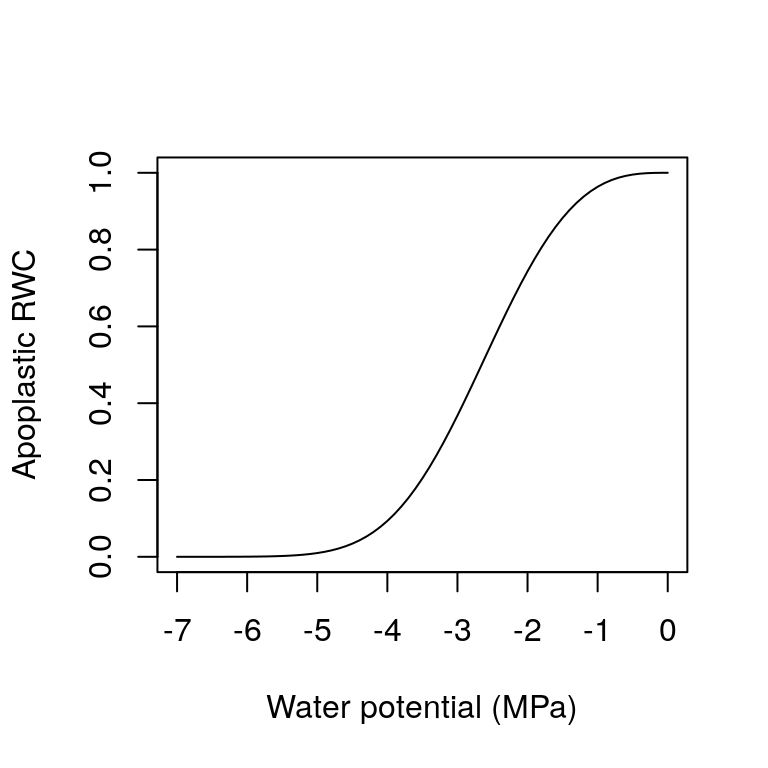
\includegraphics{medfatebook_files/figure-latex/unnamed-chunk-20-1} \end{center}

\hypertarget{water-content-of-plant-tissues}{%
\section{Water content of plant tissues}\label{water-content-of-plant-tissues}}

In \textbf{medfate} the water content of leaves and stems is tracked explicitly. Following \citet{Martin-StPaul2017}, we consider two sources of water in plant segments \citep{Tyree1990}. The first comes from the conduits (tracheids or vessels), which will release water due to cavitation and may be refilled with water from adjacent living tissue. The second source of water is formed by more elastic living cells (i.e.~parenchyma) and can potentially be a large source of water during relatively high water potentials. This source can be described using the relative water content of a symplasmic tissue. This storage compartment has its own water potential and exchanges water with the xylem conduits according to the difference in water potential.

\hypertarget{pressure-volume-curves}{%
\subsection{Pressure-volume curves}\label{pressure-volume-curves}}

A pressure-volume curve of a tissue relates a water potential against relative water content (\(RWC\); \(kg H_2O \cdot kg^{-1}H_2O\) at saturation) in drying tissues. Pressure-volume theory is usually applied to leaves \citep{Bartlett2012}, but it can also be applied to other tissues such as sapwood or cambium cells.

For living cells, the relationship between \(\Psi\) and \(RWC\) of the symplasmic fraction (\(RWC_{sym}\)) is achieved by separating \(\Psi\) into osmotic (solute) potential (\(\Psi_{S}\)) and the turgor potential (\(\Psi_{P}\)):
\begin{equation}
\Psi = \Psi_{S} + \Psi_{P}
\end{equation}
The relationship for \(\Psi_{P}\) is:
\begin{equation}
\Psi_{P} = -\pi_0 -\epsilon\cdot (1.0 - RWC_{sym})
\end{equation}
where \(\pi_0\) (MPa) is the osmotic potential at full turgor (i.e.~when \(RWC_{sym} = 1\)), and \(\epsilon\) is the modulus of elasticity (i.e.~the slope of the relationship). Assuming constant solute content, the relationship for \(\Psi_{S}\) is:
\begin{equation}
\Psi_{S} = \frac{-\pi_0}{RWC_{sym}} 
\end{equation}
When \(\Psi \leq \Psi_{tlp}\), the water potential at turgor loss point, then \(\Psi_{P} = 0\) and \(\Psi = \Psi_{S}\). If \(\Psi > \Psi_{tlp}\) then the two components are needed. The water potential at turgor loss point (\(\Psi_{tlp}\)) can be found by \citep{Bartlett2012}:
\begin{equation}
\Psi_{tlp} = \frac{\pi_0 \cdot \epsilon}{\pi_0 + \epsilon}
\end{equation}
As an example, the following figure draws the pressure-volume curve for a tissue with \(\epsilon = 12\) and \(\pi_0 = -3.0\)MPa:

\begin{center}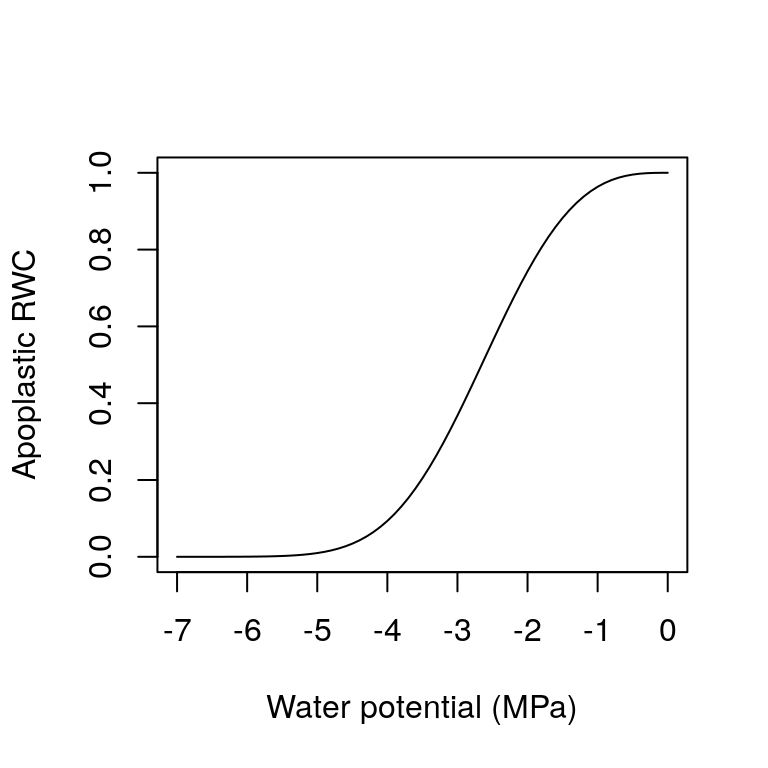
\includegraphics{medfatebook_files/figure-latex/unnamed-chunk-21-1} \end{center}

To calculate \(RWC_{sym}\) from the water potential of a tissue, the previous equations need to be combined and, after isolating \(RWC_{sym}\), a quadratic relationship is obtained.

Apoplastic reservoirs (e.g.~sapwood) consist of inelastic cells that release their water to the transpiration stream following embolism. As in \citet{Holtta2009}, we equate the relative water content of the apoplastic reservoir of a segment (leaves or stem) to the proportion of maximum conductance in the vulnerability curve:
\begin{equation}
RWC_{apo}(\Psi) = \frac{k(\Psi)}{k_{max}} = e^{-((\Psi/d)^{c})}
\end{equation}

\begin{center}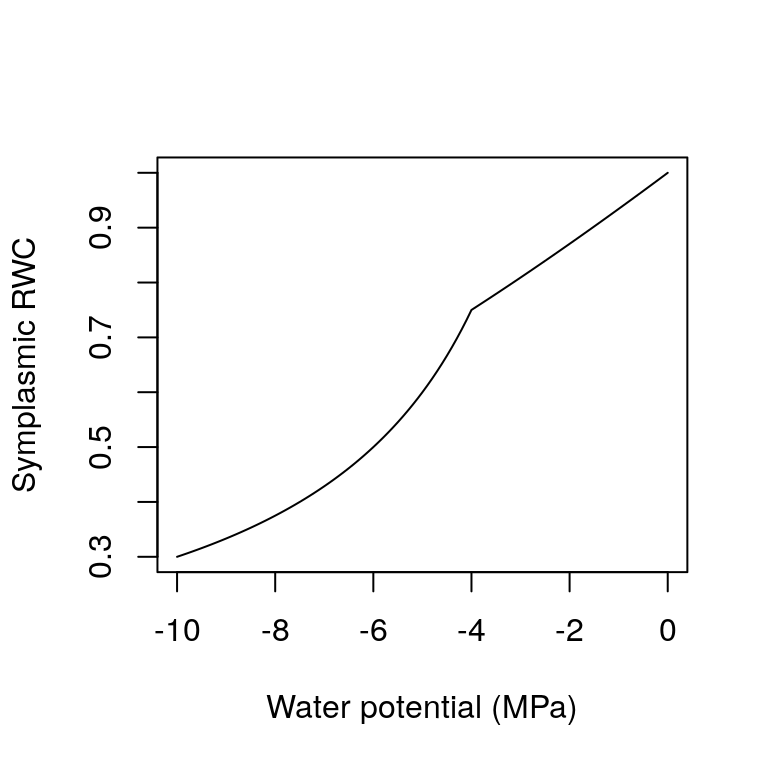
\includegraphics{medfatebook_files/figure-latex/unnamed-chunk-22-1} \end{center}

The average relative water content in a given compartment (\(RWC\)) can be obtained from \(\Psi_{sym}\) and \(\Psi_{apo}\) by calculating \(RWC_{sym}(\Psi_{sym})\) and \(RWC_{apo}(\Psi_{apo})\) followed by assuming a constant apoplastic fraction \(f_{apo}\):
\begin{equation}
RWC = RWC_{apo}(\Psi_{apo}) \cdot f_{apo} + RWC_{sym}(\Psi_{sym}) \cdot (1 - f_{apo})
\end{equation}

\hypertarget{water-content-and-live-fuel-moisture-content}{%
\subsection{Water content and live fuel moisture content}\label{water-content-and-live-fuel-moisture-content}}

Pressure-volume curves are useful to determine the moisture content of live fuel elements (leaves and twigs). Given an average relative water content of a water compartment, its live fuel moisture content (\(LFMC\) in \(g H_2O \cdot g^{-1}\) of dry tissue) can be calculated using:
\begin{equation}
LFMC = RWC \cdot \Theta \cdot \frac{\rho_{H_2O}}{\rho} = RWC \cdot LFMC_{max}
\end{equation}
where \(\Theta\) is the tissue porosity (\(cm^3\) of water per \(cm^3\) of tissue), \(\rho\) is the density of the tissue and \(\rho_{H_2O}\) is the density of water.

If we know \(RWC_{apo}(\Psi_{apo})\), the relative water content in conduits, and \(V_{segment}\) (in \(m^3\)), the volume of conducting tissue (sapwood) in the segment, then the mass of water that is stored in conduits is:
\begin{equation}
S_{apo}(\Psi_{apo}) = V_{segment} \cdot f_{apo} \cdot RWC_{apo}(\Psi_{apo}) \cdot \rho_{w}
\end{equation}
where \(\rho_{w}\) is the density of water (\(kgH_2O \cdot m^{-3}\)) and \(f_{apo,s}\) is the volume fraction of apoplastic tissue within sapwood. Similarly, the amount of water stored in the symplastic tissue of the segment at any time is:
\begin{equation}
S_{sym}(\Psi_{sym}) = V_{segment} \cdot (1 - f_{apo}) \cdot RWC_{sym}(\Psi_{sym}) \cdot \rho_{w}
\end{equation}

Finally, if we consider that both apoplastic and symplastic tissues are at the same water potential, the water content in the segment will be:
\begin{equation}
S(\Psi) = V_{segment} \cdot (f_{apo} \cdot RWC_{apo}(\Psi) + (1 - f_{apo}) \cdot RWC_{sym}(\Psi)) \cdot \rho_{w}
\end{equation}

\hypertarget{relative-water-content-and-cavitation}{%
\subsection{Relative water content and cavitation}\label{relative-water-content-and-cavitation}}

In \textbf{medfate} we assume that cavitation in stems is non-reversible. Within a given sapwood segment, we further assume that the proportion of conductance loss (\(PLC\)) is related to the relative water content (\(RWC\)) in its conduit vessels (i.e.~the water volume in conduit vessels with respect to the maximum water volume):
\begin{equation}
PLC(\Psi_{cav}) = 1 - RWC_{apo}(\Psi_{cav})
\end{equation}
where \(RWC_{apo,s}\) is the function of relative water content for apoplastic stem tissue. With this assumption one can relate changes in PLC derived from cavitation with decreases in water content in xylem conduits. When \(PLC\) increases the associated change in water content is a source of water can be added to the transpirational stream \citep{Martin-StPaul2017}.

\hypertarget{supply-functions}{%
\section{Supply functions}\label{supply-functions}}

The supply function describes the rate of water supply (i.e.~flow) for transpiration (\(E\)) as a function of pressure. The steady-state flow rate \(E_i\) through each \(i\) element of the continuum is related to the flow-induced drop in pressure across that element (\(\Delta \Psi_i\)) by the integral transform of the element's vulnerability curve \(k_i(\Psi)\) \citep{Sperry2015}:
\begin{equation}
E_i(\Delta \Psi_i) = \int_{\Psi_{up}}^{\Psi_{down}}{k_i(\Psi) d\Psi}
\label{eq:generalsupply}
\end{equation}
where \(\Psi_{up}\) and \(\Psi_{down}\) are the upstream and downstream water potential values, respectively. The integral transform assumes infinite discretization of the flow path. The supply function can be defined for individual elements of the continuum or for the whole soil-plant continuum using different topologies. In the following subsections we illustrate the supply function for different cases.

\hypertarget{supply-function-for-single-elements}{%
\subsection{Supply function for single elements}\label{supply-function-for-single-elements}}

In the case of a single stem xylem element the supply function describes the flow rate as a function of canopy pressure (\(\Psi_{canopy}\)). It can be calculated by numerical integration or aproximated using an incomplete gamma function. The shape of the supply function starting at different root crown water potential values (\(\Psi_{rootcrown}\)) is (see function \texttt{hydraulics\_EXylem()}):

\begin{center}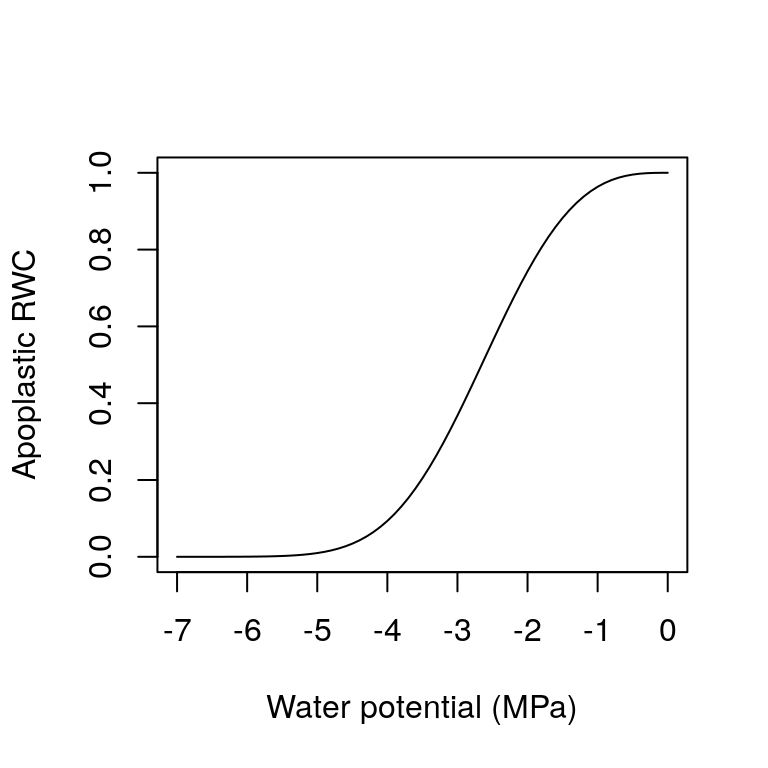
\includegraphics{medfatebook_files/figure-latex/unnamed-chunk-23-1} \end{center}

Right pane shows the supply functions that are obtained in the case of a cavitated xylem (i.e.~without refilling), assuming that the minimum water potential experienced so far was -2.5 MPa. Note the linear part of the flow rate between \(\Psi_{soil}\) and this limit.

The supply function of the rhizosphere element relates the flow rate to the pressure inside the roots (\(\Psi_{root}\)). It is calculated by numerical integration of the van Genuchten function (see function \texttt{hydraulics\_EVanGenuchten()}), for which we use the analytical approximation of \citet{VanLier2009}. Here we draw the supply function for the rhizosphere starting at the four different values of bulk soil pressure (\(\Psi_{soil}\)) and for the same three texture types:

\begin{center}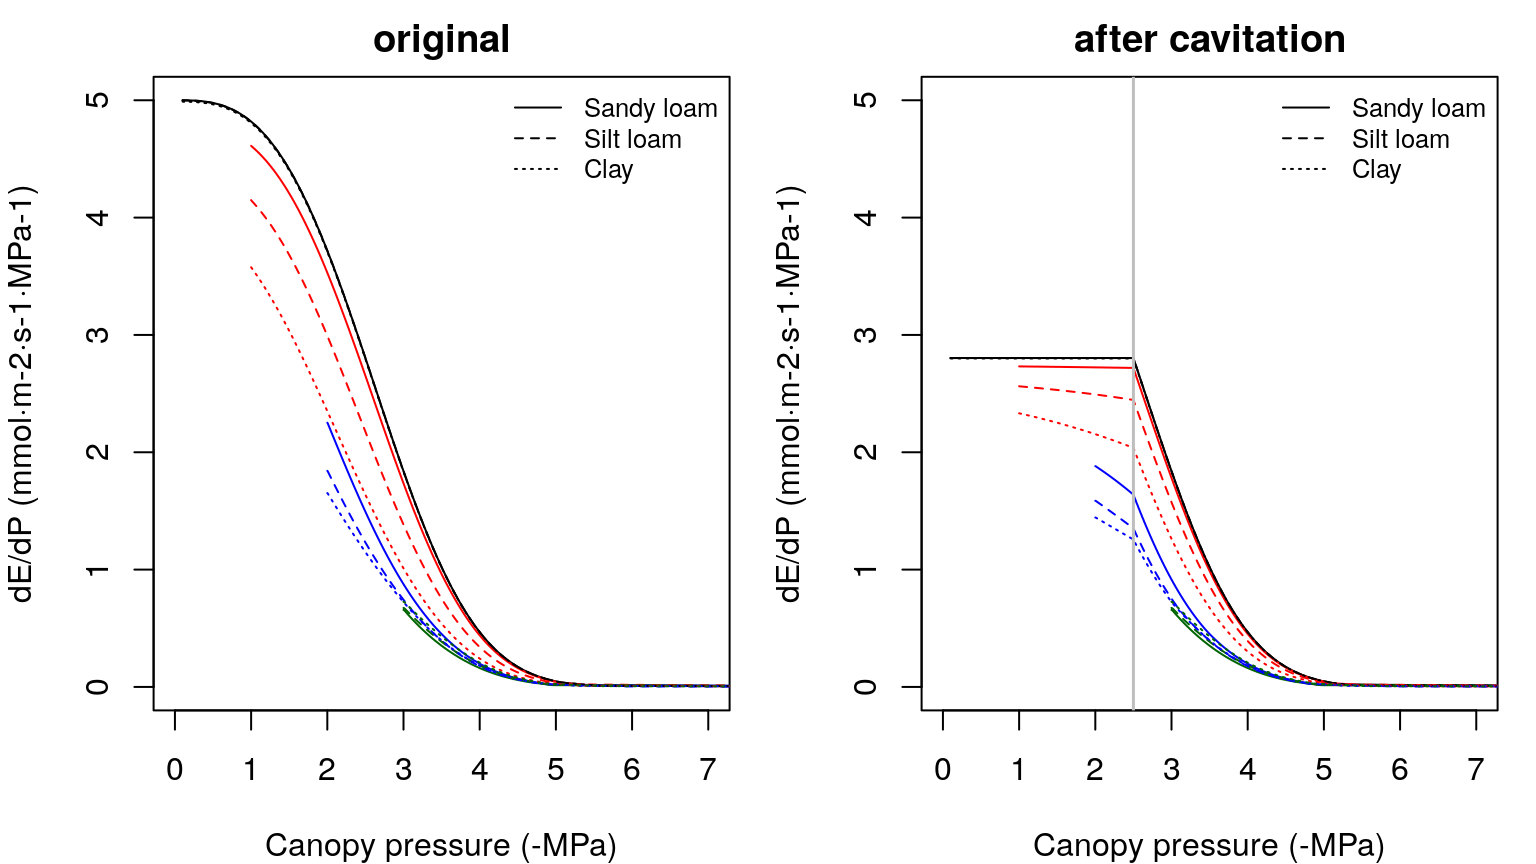
\includegraphics{medfatebook_files/figure-latex/unnamed-chunk-24-1} \end{center}

The nearly vertical lines indicate that for many values of \(E_i\) the corresponding drop in water potential through the rhizosphere will be negligible. Only for increasingly negative soil water potential values the decrease in water potential through the rhizosphere becomes relevant. Both in the case of a xylem element or a rhyzosphere element the derivative \(dE_i/d\Psi\) of the supply function is equal to the corresponding vulnerability curve.

\hypertarget{supply-function-of-two-elements-in-series}{%
\subsection{Supply function of two elements in series}\label{supply-function-of-two-elements-in-series}}

Let us describe the soil-plant continuum is represented using \emph{two} elements in series (rhizosphere + stem xylem). In this case, the supply function has to be calculated by sequentially using the previous supply functions. The \(E_i\) is identical for each element and equal to the canopy \(E\). Since \(\Psi_{soil}\) is known, one first inverts the supply function of the rhizosphere to find \(\Psi_{root}\) (see function \texttt{hydraulics\_E2psiVanGenuchten()}) and then inverts the supply function of the xylem to find \(\Psi_{canopy}\) (see function \texttt{hydraulics\_E2psiXylem()}). The two operations can be summarized in a single supply function describing the potential rate of water supply for transpiration (\(E\)) as function of the canopy xylem pressure (\(\Psi_{canopy}\)), starting from different bulk soil (\(\Psi_{soil}\)) values (see function \texttt{hydraulics\textbackslash{}\_supplyFunctionTwoElements()}):

\begin{center}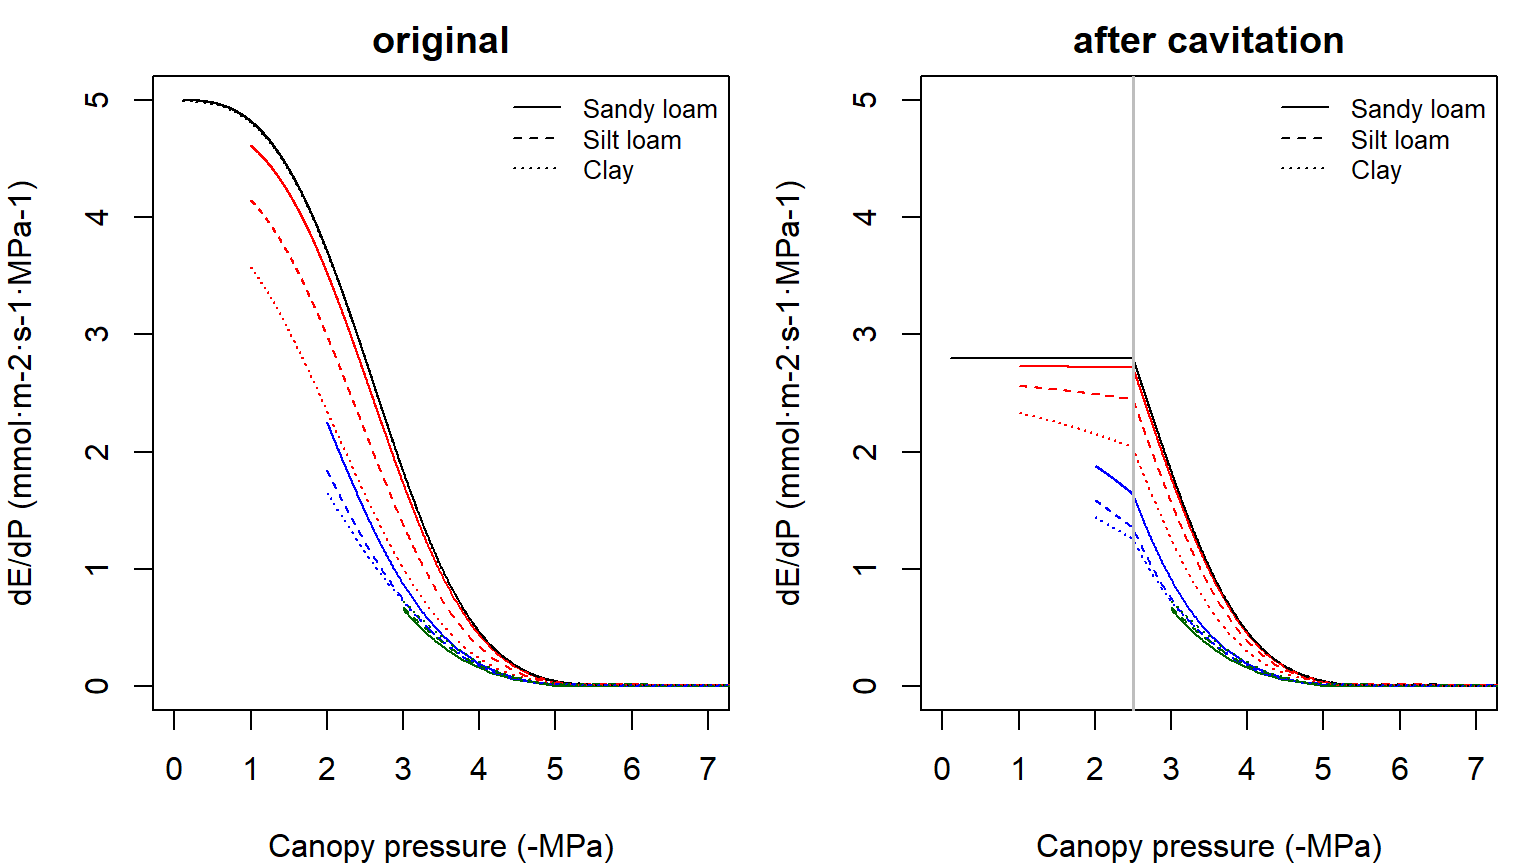
\includegraphics{medfatebook_files/figure-latex/unnamed-chunk-25-1} \end{center}

The supply function for the whole continuum contains much information. The \(\Psi\) intercept at \(E=0\) represents the predawn canopy sap pressure which integrates the rooted soil moisture profile. As \(E\) increments from zero, the disproportionately greater drop in \(\Psi_{canopy}\) results from the loss of conductance. As the soil dries the differences in flow due to soil texture become more apparent. The derivative of the whole continuum supply function, \(dE/d\Psi\), is not equal to either of the vulnerability curves and it has to be obtained numerically. The derivative functions corresponding to the supply functions shown in the previous figure are:

\begin{center}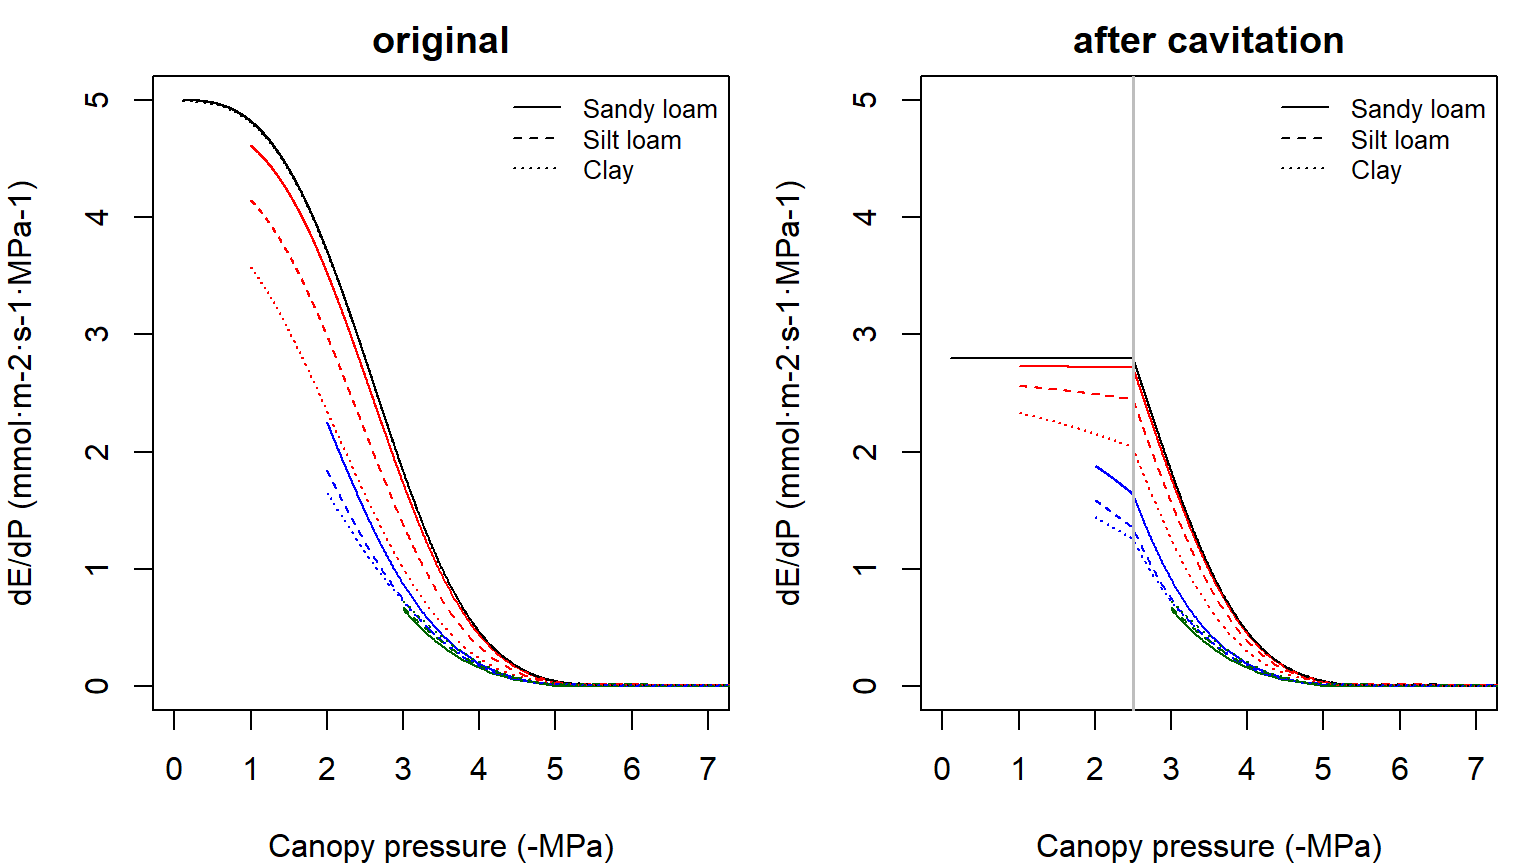
\includegraphics{medfatebook_files/figure-latex/unnamed-chunk-26-1} \end{center}

The derivative \(dE/d\Psi_{canopy}\) is the conductance if the entire continuum was exposed to \(\Psi_{canopy}\) \citep{Sperry2015}. It corresponds to the local loss of hydraulic conductance at the downstream end of the flow path. It falls towards zero for asymptotic critical values (\(E_{crit}\)). For a cavitated system \(dE/d\Psi_{canopy}\) can be rather flat, in accordance with the close to linear part of the supply function.

\hypertarget{supply-function-of-three-elements-in-series}{%
\subsection{Supply function of three elements in series}\label{supply-function-of-three-elements-in-series}}

If the soil-plant continuum is represented using \emph{three} elements in series (rhizosphere + stem xylem + leaf), the resulting overall conductance and resistance fractions (under wet conditions) are:

\begin{Shaded}
\begin{Highlighting}[]
\NormalTok{rstemmin =}\StringTok{ }\DecValTok{1}\OperatorTok{/}\NormalTok{kstemmax}
\NormalTok{rleafmin =}\StringTok{ }\DecValTok{1}\OperatorTok{/}\NormalTok{kleafmax}

\CommentTok{#Percentages of minimum resistance}
\NormalTok{rvec =}\StringTok{ }\KeywordTok{c}\NormalTok{(rstemmin,rleafmin)}
\DecValTok{100}\OperatorTok{*}\NormalTok{rvec}\OperatorTok{/}\KeywordTok{sum}\NormalTok{(rvec)}
\end{Highlighting}
\end{Shaded}

\begin{verbatim}
## [1] 66.66667 33.33333
\end{verbatim}

\begin{Shaded}
\begin{Highlighting}[]
\CommentTok{#Maximum overall conductance}
\DecValTok{1}\OperatorTok{/}\KeywordTok{sum}\NormalTok{(rvec)}
\end{Highlighting}
\end{Shaded}

\begin{verbatim}
## [1] 3.333333
\end{verbatim}

As before, the supply function has to be calculated by sequentially. The \(E_i\) is identical for each element. Since \(\Psi_{soil}\) is known, one first inverts the supply function of the rhizosphere to find \(\Psi_{root}\) and then inverts the supply function of the xylem to find \(\Psi_{stem}\). Finally, one inverts the supply function of the leaf element to find \(\Psi_{leaf}\). As before, the three operations can be summarized in a single supply function describing the potential rate of water supply for transpiration (\(E\)) as function of the leaf pressure (\(\Psi_{leaf}\)), starting from different bulk soil (\(\Psi_{soil}\)) values (see function \texttt{hydraulics\_supplyFunctionThreeElements()}):

\begin{center}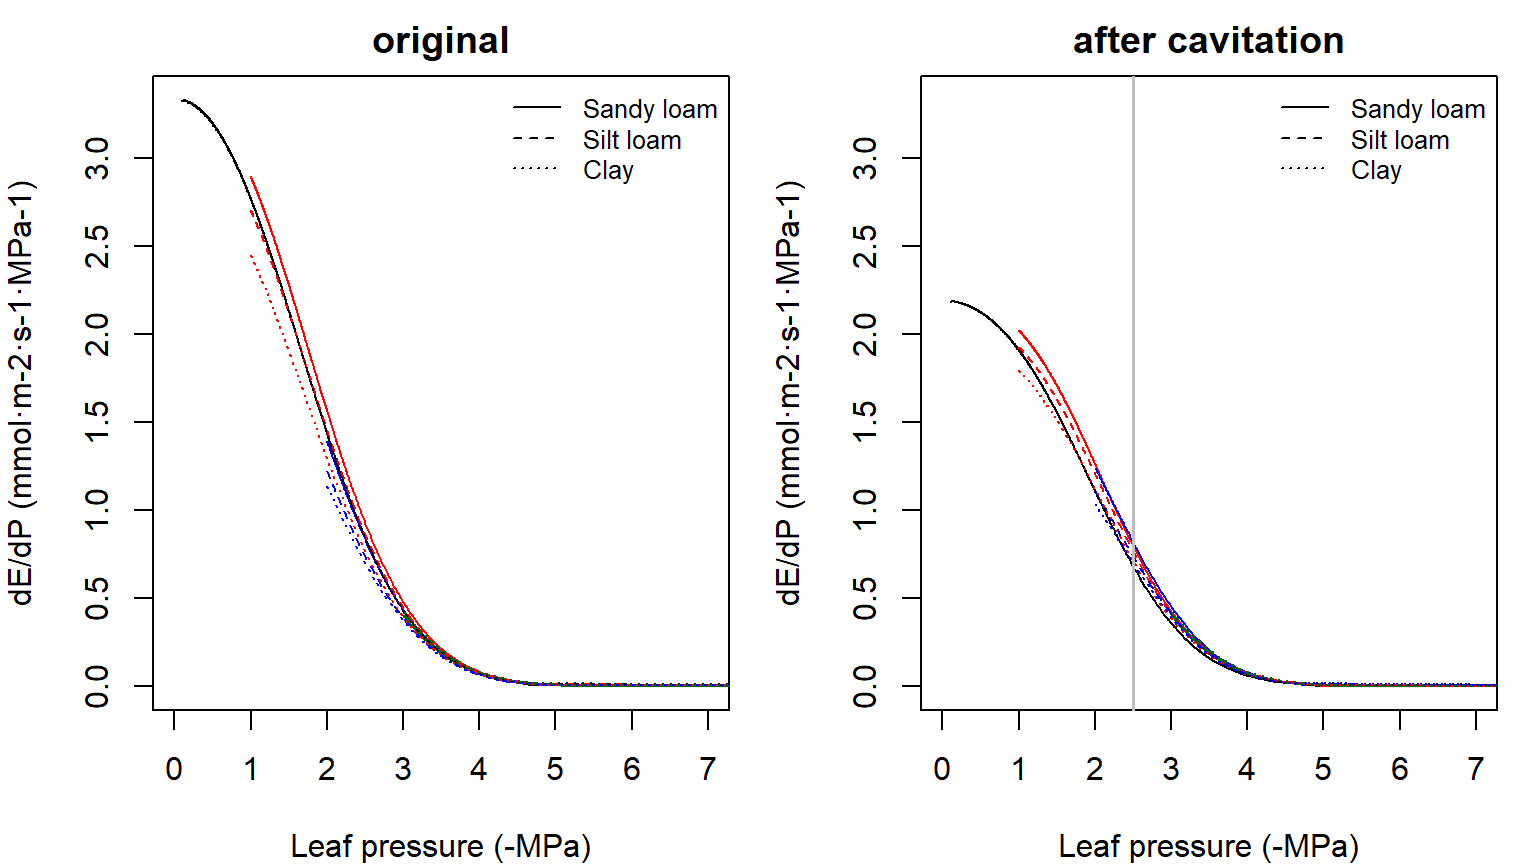
\includegraphics{medfatebook_files/figure-latex/unnamed-chunk-28-1} \end{center}

Note that overall conductance and the maximum flow of the supply function are smaller in this case than in the representation using two elements in series. While the rhizosphere component only adds a significant resistance when the soil dries, considering the leaf segment (or a root xylem segment) increases the overall resistance of the continuum. Higher vulnerability of leaves also makes the curve to saturate for less negative soil water potentials. The derivative functions corresponding to the supply functions shown in the previous figure are (note the highest value being equal to the overall maximum conductance):

\begin{center}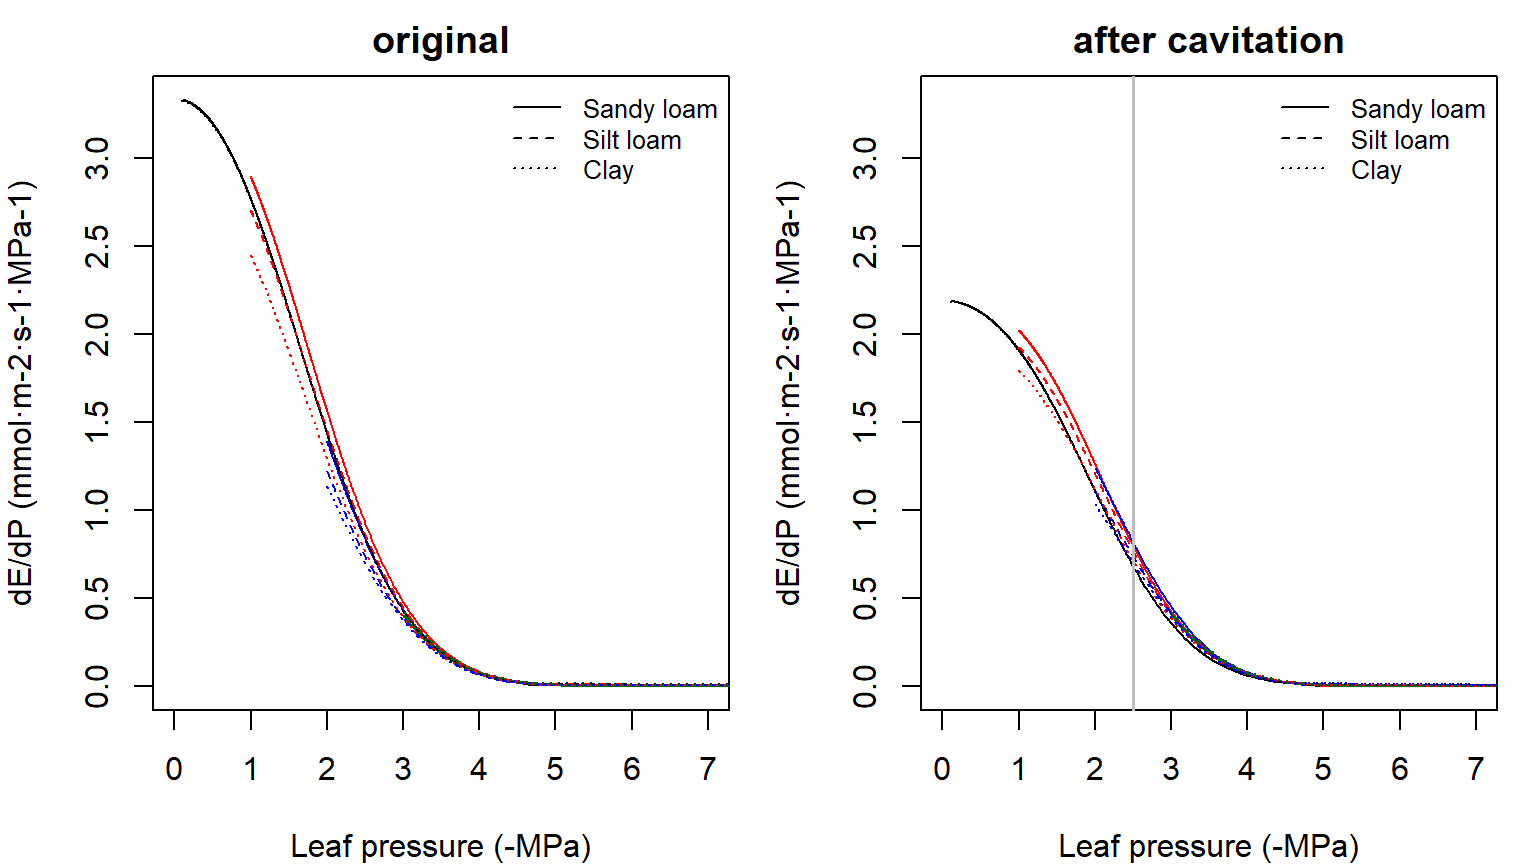
\includegraphics{medfatebook_files/figure-latex/unnamed-chunk-29-1} \end{center}

\hypertarget{supply-function-of-a-root-system}{%
\subsection{Supply function of a root system}\label{supply-function-of-a-root-system}}

So far we considered supply functions of elements in series, but resistance elements will be in parallel if soil is represented using \(N>1\) different layers. For each soil layer there is a rhizosphere element in series with a root xylem element. The \(N\) soil layers are in parallel up to the root crown.

Network of \(N\) rhizosphere components and root layers in parallel there are \(N+1\) unknown pressures: the \(N\) root surface pressures (\(\Psi_{rootsurf,1},\dots,\Psi_{rootsurf,N}\)) and the root crown pressure at the downstream junction for all root components (\(\Psi_{rootcrown}\)). The \(N+1\) unknown pressures are solved, for each specified total flow value \(E\), using multidimensional Newton-Raphson on a set of equations for steady-state flow \citep{Sperry2016a}:
\begin{eqnarray}
   E_{k, rhizosphere}-E_{k,root} &=& 0 \\
   \sum_{k}^{n}{E_{k,root}}-E &=& 0
\end{eqnarray}
where \(E_{k, rhizosphere}\) and \(E_{k, root}\) are supply flows calculated using the integrals of either van Genuchten or Weibull function as vulnerability curves, respectively. In the case of rhizosphere elements, \(\Psi_{up,k}=\Psi_{soil,k}\) and in the case of root elements \(\Psi_{up,k}=\Psi_{rootsurf,k}\). Solving the steady-state equations also provides values for flow across each of the parallel paths \(E_{k, rhizosphere} = E_{k, root}\), which are useful to conduct water balance operations on each layer.

\begin{figure}

{\centering 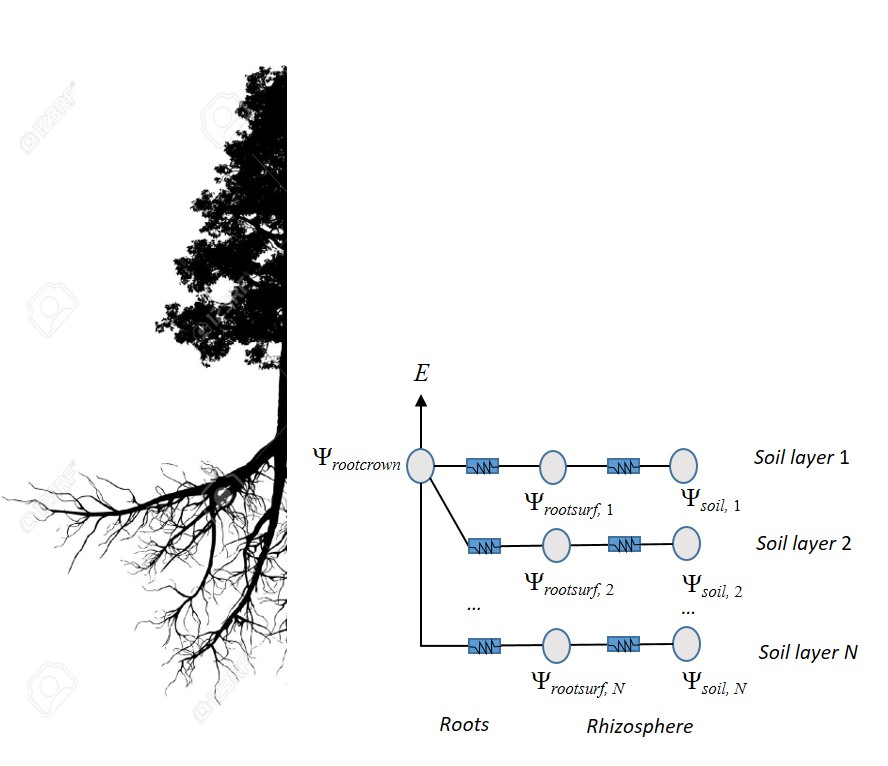
\includegraphics[width=0.8\linewidth]{hydraulics_rs} 

}

\caption{Schematic representation of hydraulics in a root network}\label{fig:unnamed-chunk-30}
\end{figure}

As an example, we start by defining the water potential of three soil layers corresponding to four situations (analogously with the soil water potentials defined above):

\begin{Shaded}
\begin{Highlighting}[]
\NormalTok{ psiSoilLayers1 =}\StringTok{ }\KeywordTok{c}\NormalTok{(}\OperatorTok{-}\FloatTok{0.3}\NormalTok{,}\OperatorTok{-}\FloatTok{0.2}\NormalTok{,}\OperatorTok{-}\FloatTok{0.1}\NormalTok{)}
\NormalTok{ psiSoilLayers2 =}\StringTok{ }\KeywordTok{c}\NormalTok{(}\OperatorTok{-}\FloatTok{1.3}\NormalTok{,}\OperatorTok{-}\FloatTok{1.2}\NormalTok{,}\OperatorTok{-}\FloatTok{1.1}\NormalTok{)}
\NormalTok{ psiSoilLayers3 =}\StringTok{ }\KeywordTok{c}\NormalTok{(}\OperatorTok{-}\FloatTok{2.3}\NormalTok{,}\OperatorTok{-}\FloatTok{2.2}\NormalTok{,}\OperatorTok{-}\FloatTok{2.1}\NormalTok{)}
\NormalTok{ psiSoilLayers4 =}\StringTok{ }\KeywordTok{c}\NormalTok{(}\OperatorTok{-}\FloatTok{3.3}\NormalTok{,}\OperatorTok{-}\FloatTok{3.2}\NormalTok{,}\OperatorTok{-}\FloatTok{3.1}\NormalTok{)}
\end{Highlighting}
\end{Shaded}

In a network of several soil layers, one has to divide the total rhizosphere and root xylem conductances among layers. Let layer depths be:

\begin{Shaded}
\begin{Highlighting}[]
\NormalTok{d =}\StringTok{ }\KeywordTok{c}\NormalTok{(}\DecValTok{300}\NormalTok{,}\DecValTok{700}\NormalTok{,}\DecValTok{3000}\NormalTok{) }\CommentTok{#Soil layer widths in mm}
\end{Highlighting}
\end{Shaded}

Now let \(v_1\), \(v_2\) and \(v_3\) be the proportion of fine root biomass in each soil layer.

\begin{Shaded}
\begin{Highlighting}[]
\NormalTok{Z50 =}\StringTok{ }\DecValTok{200} \CommentTok{#Parameter of LDR root distribution}
\NormalTok{Z95 =}\StringTok{ }\DecValTok{1200} \CommentTok{#Parameter of LDR root distribution}
\NormalTok{v =}\StringTok{ }\KeywordTok{root_ldrDistribution}\NormalTok{(Z50, Z95, d)}
\NormalTok{v}
\end{Highlighting}
\end{Shaded}

\begin{verbatim}
##           [,1]      [,2]       [,3]
## [1,] 0.6652935 0.2749944 0.05971209
\end{verbatim}

In the case of the rhizosphere conductances, we can simply define them (for each soil texture type) as:

\begin{Shaded}
\begin{Highlighting}[]
\NormalTok{krhizomaxvec1 =}\StringTok{ }\NormalTok{krmax1}\OperatorTok{*}\NormalTok{v}
\NormalTok{krhizomaxvec2 =}\StringTok{ }\NormalTok{krmax2}\OperatorTok{*}\NormalTok{v}
\NormalTok{krhizomaxvec3 =}\StringTok{ }\NormalTok{krmax3}\OperatorTok{*}\NormalTok{v}
\end{Highlighting}
\end{Shaded}

To divide maximum root xylem conductance among soil layers we need weights inversely proportional to the length of transport distances \citep{Sperry2016a}. Vertical transport lengths can be calculated from soil depths and radial spread can be calculated assuming cylinders with volume proportional to the proportions of fine root biomass. The whole process can be done using function \texttt{root\_rootXylemConductanceProportions()}:

\begin{Shaded}
\begin{Highlighting}[]
\NormalTok{weights =}\StringTok{ }\KeywordTok{root_xylemConductanceProportions}\NormalTok{(v, d)}
\NormalTok{weights}
\end{Highlighting}
\end{Shaded}

\begin{verbatim}
## [1] 0.2369724 0.4214326 0.3415950
\end{verbatim}

Transport weights are quite different than the fine root biomass proportions. This is because radial lengths are largest for the first (top) layer and vertical lengths are largest for the third (bottom) layer. The root xylem conductances are (in this case they do not depend on soil texture):

\begin{Shaded}
\begin{Highlighting}[]
\NormalTok{krootmaxvec =}\StringTok{ }\NormalTok{krootmax}\OperatorTok{*}\NormalTok{weights}
\NormalTok{krootmaxvec}
\end{Highlighting}
\end{Shaded}

\begin{verbatim}
## [1] 1.564018 2.781455 2.254527
\end{verbatim}

Having all these maximum conductances, we can now build the supply functions for each soil texture and starting from the different soil water potential configurations (see function \texttt{hydraulics\_supplyFunctionBelowground()}):

\begin{center}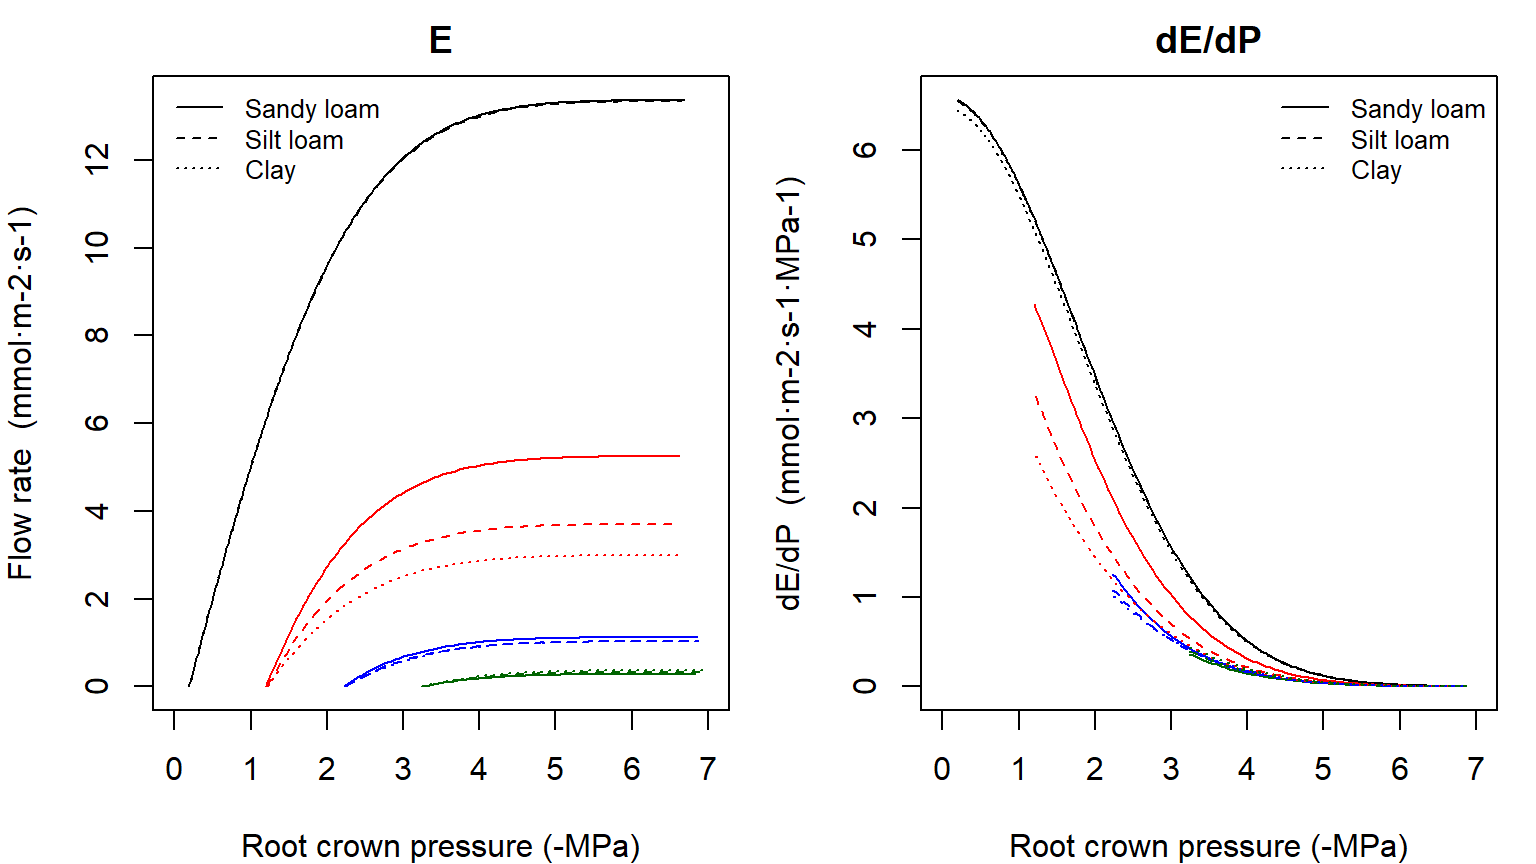
\includegraphics{medfatebook_files/figure-latex/unnamed-chunk-37-1} \end{center}

The derivative of \(dE/d\Psi_{rootcrown}\) for the supply function of the root system is again obtained numerically. Solving the previous system of equations provides the water potentials in different points of the root system. Here we plot them for the results of silt loam texture and the first and last soil potential vectors defined above:

\begin{center}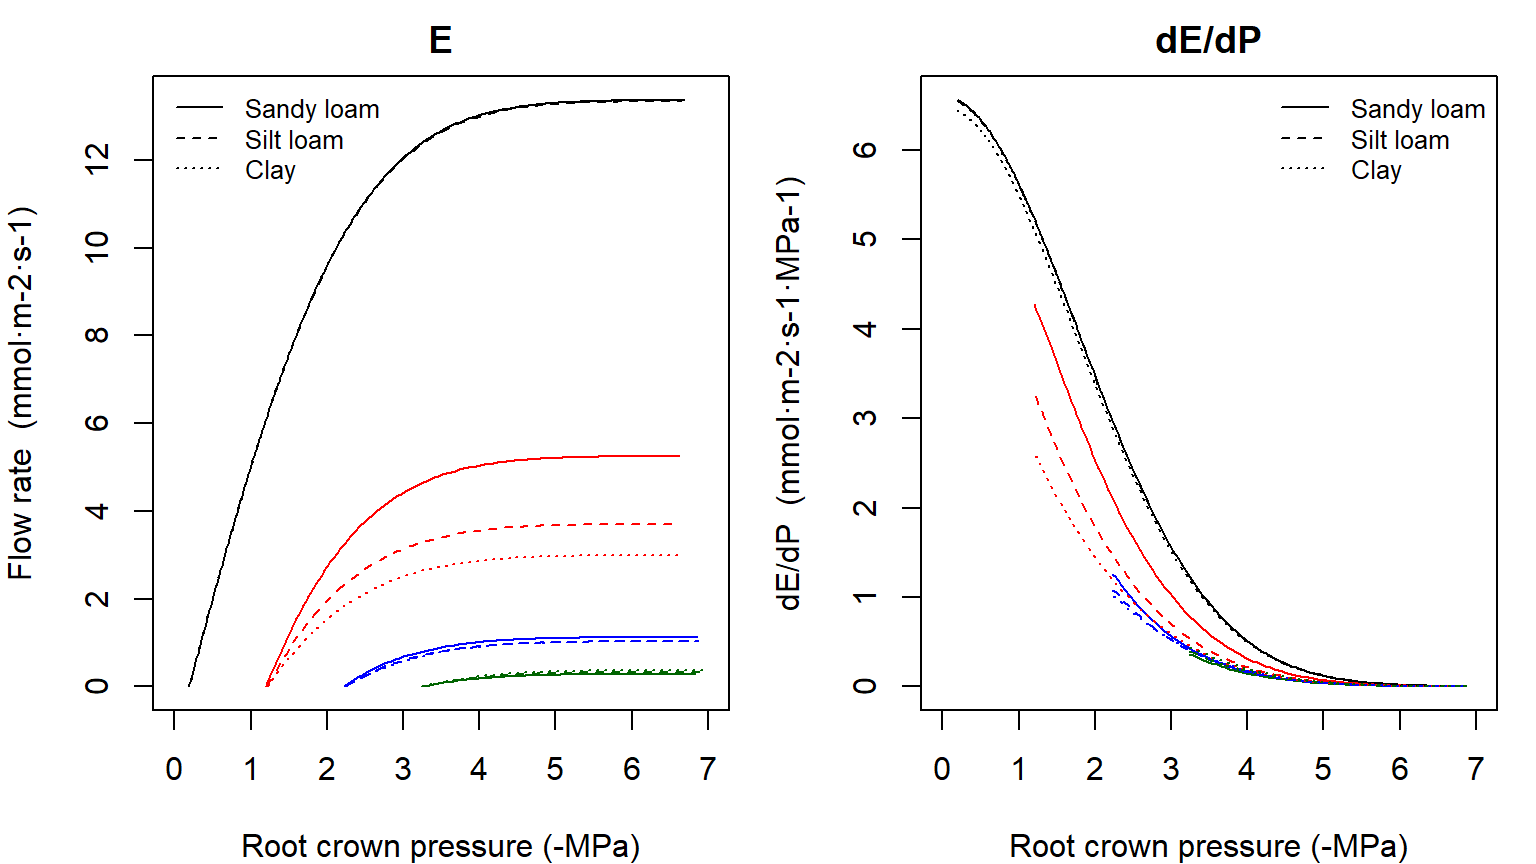
\includegraphics{medfatebook_files/figure-latex/unnamed-chunk-38-1} \end{center}

Note that when soil is not dry (first situation) pressure drop in the rhizosphere is negligible, but not the pressure drop in the root xylem. For drier soils rhizosphere becomes more relevant. We can also plot the flow rates across each of the parallel paths (again corresponding to the results of silt loam texture and for the four soil potential vectors):

\begin{center}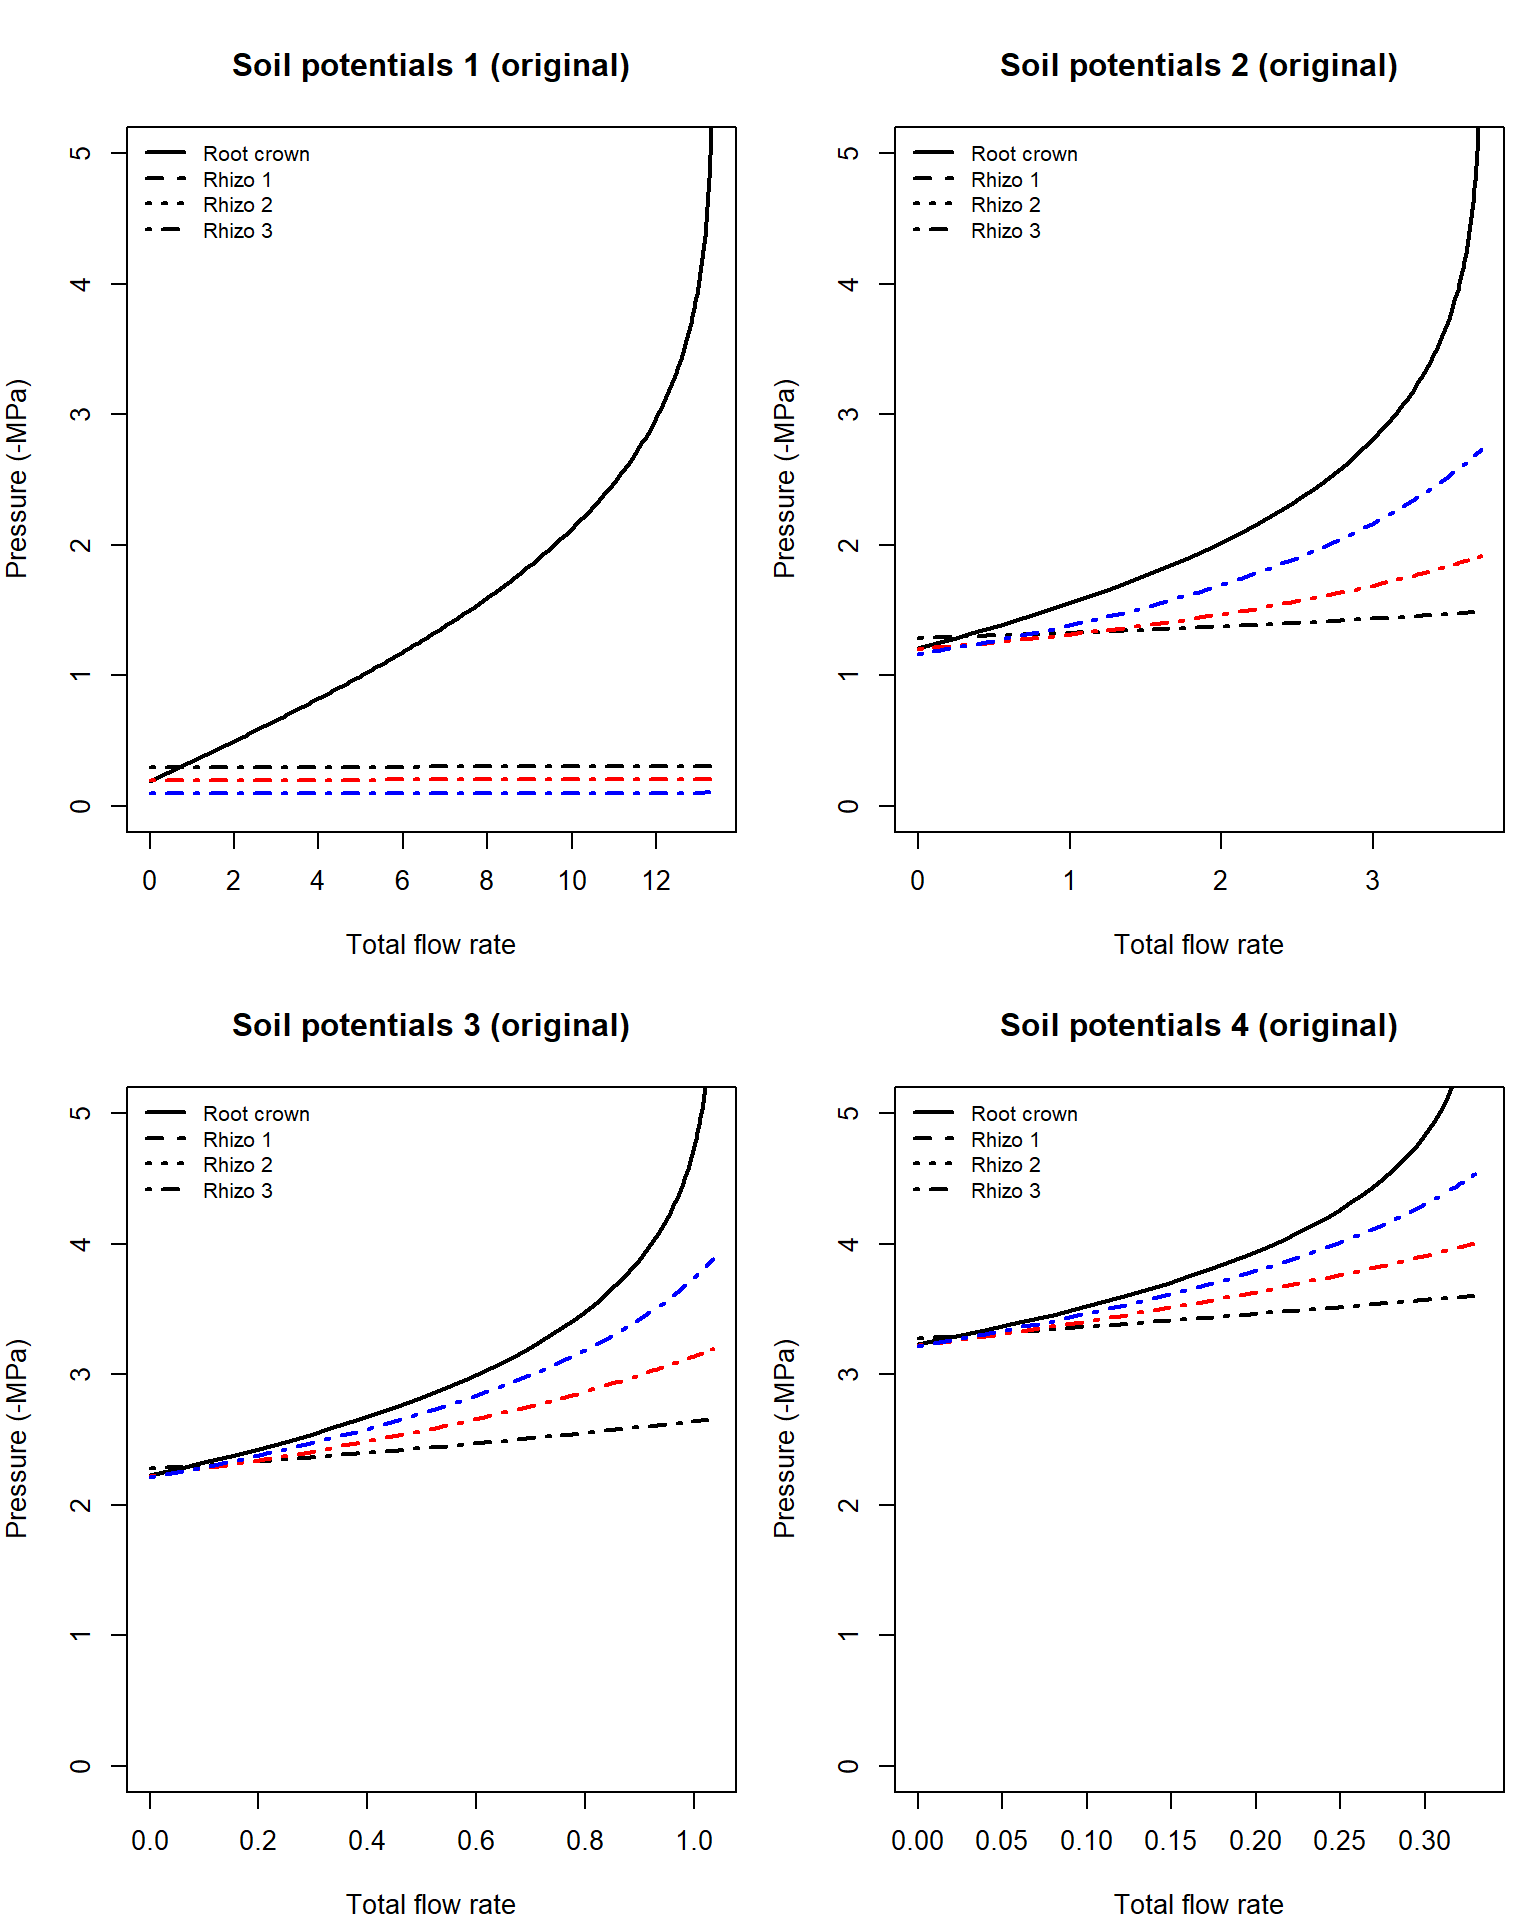
\includegraphics{medfatebook_files/figure-latex/unnamed-chunk-39-1} \end{center}

Note that the contribution of each soil layer depends on the soil conditions and the total amount of flow. For a low total flow rate some layers may have negative flows if their potential is lower than others, which in a dynamic context will cause hydraulic redistribution of water among soil layers.

\hypertarget{supply-function-of-the-soil-plant-continuum}{%
\subsection{Supply function of the soil-plant continuum}\label{supply-function-of-the-soil-plant-continuum}}

We can use a network of \((N \times 2 + S + 1)\) resistance elements to represent the soil-plant continuum, with soil being represented in \(N\) different layers. As before, the \(N\) soil layers are in parallel up to the root crown and each soil layer requires at least a rhizosphere and a root segment. From the root crown there are \(S\) stem xylem elements (normally \(S = 1\)) in series and a final leaf element. The whole hydraulic network is illustrated in the figure below.

To build the supply function for the network, we proceed by calculating water potentials in the network for each value of flow. For any given \(E\) value we start by calculating flows and potentials within the root system. After that, and assuming \(S = 1\), the water potential at the upper end of the stem (\(\Psi_{stem}\)) is obtained using the inverse of the stem supply function and setting \(\Psi_{up,k}=\Psi_{rootcrown}\). If \(S > 1\), this is done for each of the stem segments (thus obtaining \(\Psi_{stem, 1}\), \(\Psi_{stem, 2}\), \ldots{} \(\Psi_{stem, S}\)), while using a maximum conductance for segments equal to \(k_{max,s}\) times \(S\). Leaf water potential (\(\Psi_{leaf}\)) is finaly obtained using the inverse of the leaf supply function and setting \(\Psi_{up,k}=\Psi_{stem, S}\) and assuming a steady-state flow \(E\). The whole supply function \(E(\Psi_{leaf}\)) is obtained repeating these operations from \(E=0\) to a critical value \(E_{crit}\).

\begin{figure}

{\centering 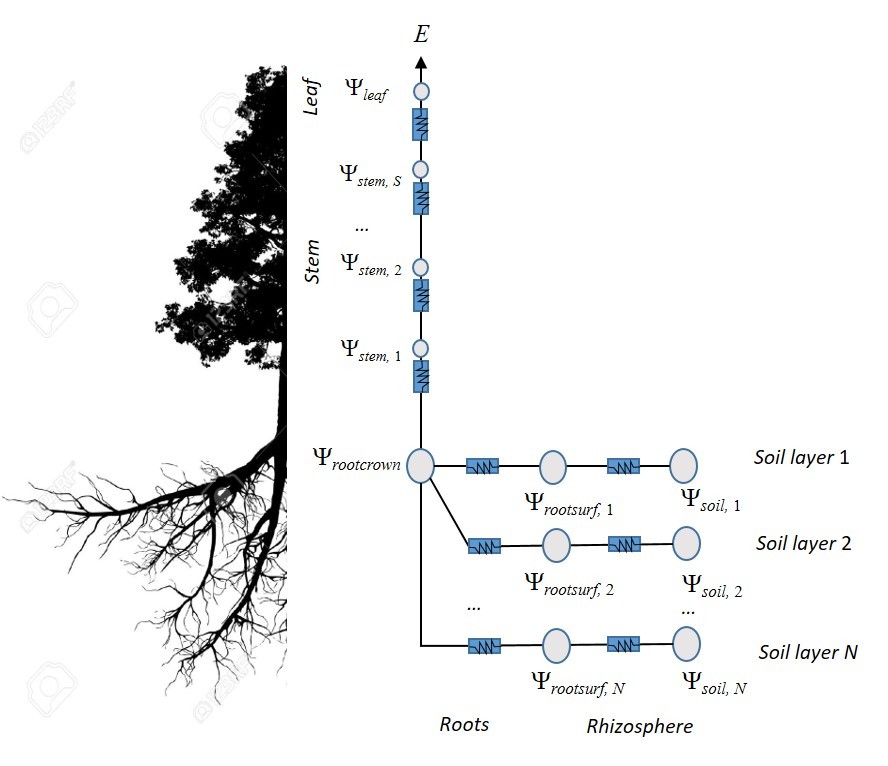
\includegraphics[width=0.8\linewidth]{hydraulics_nocap} 

}

\caption{Schematic representation of hydraulics in a whole-plant network}\label{fig:unnamed-chunk-40}
\end{figure}

The following figure shows network supply functions (with \(S = 1\)) for each soil texture and starting from the different soil water potential configurations (see function \texttt{hydraulics\_supplyFunctionNetwork()}):

\begin{center}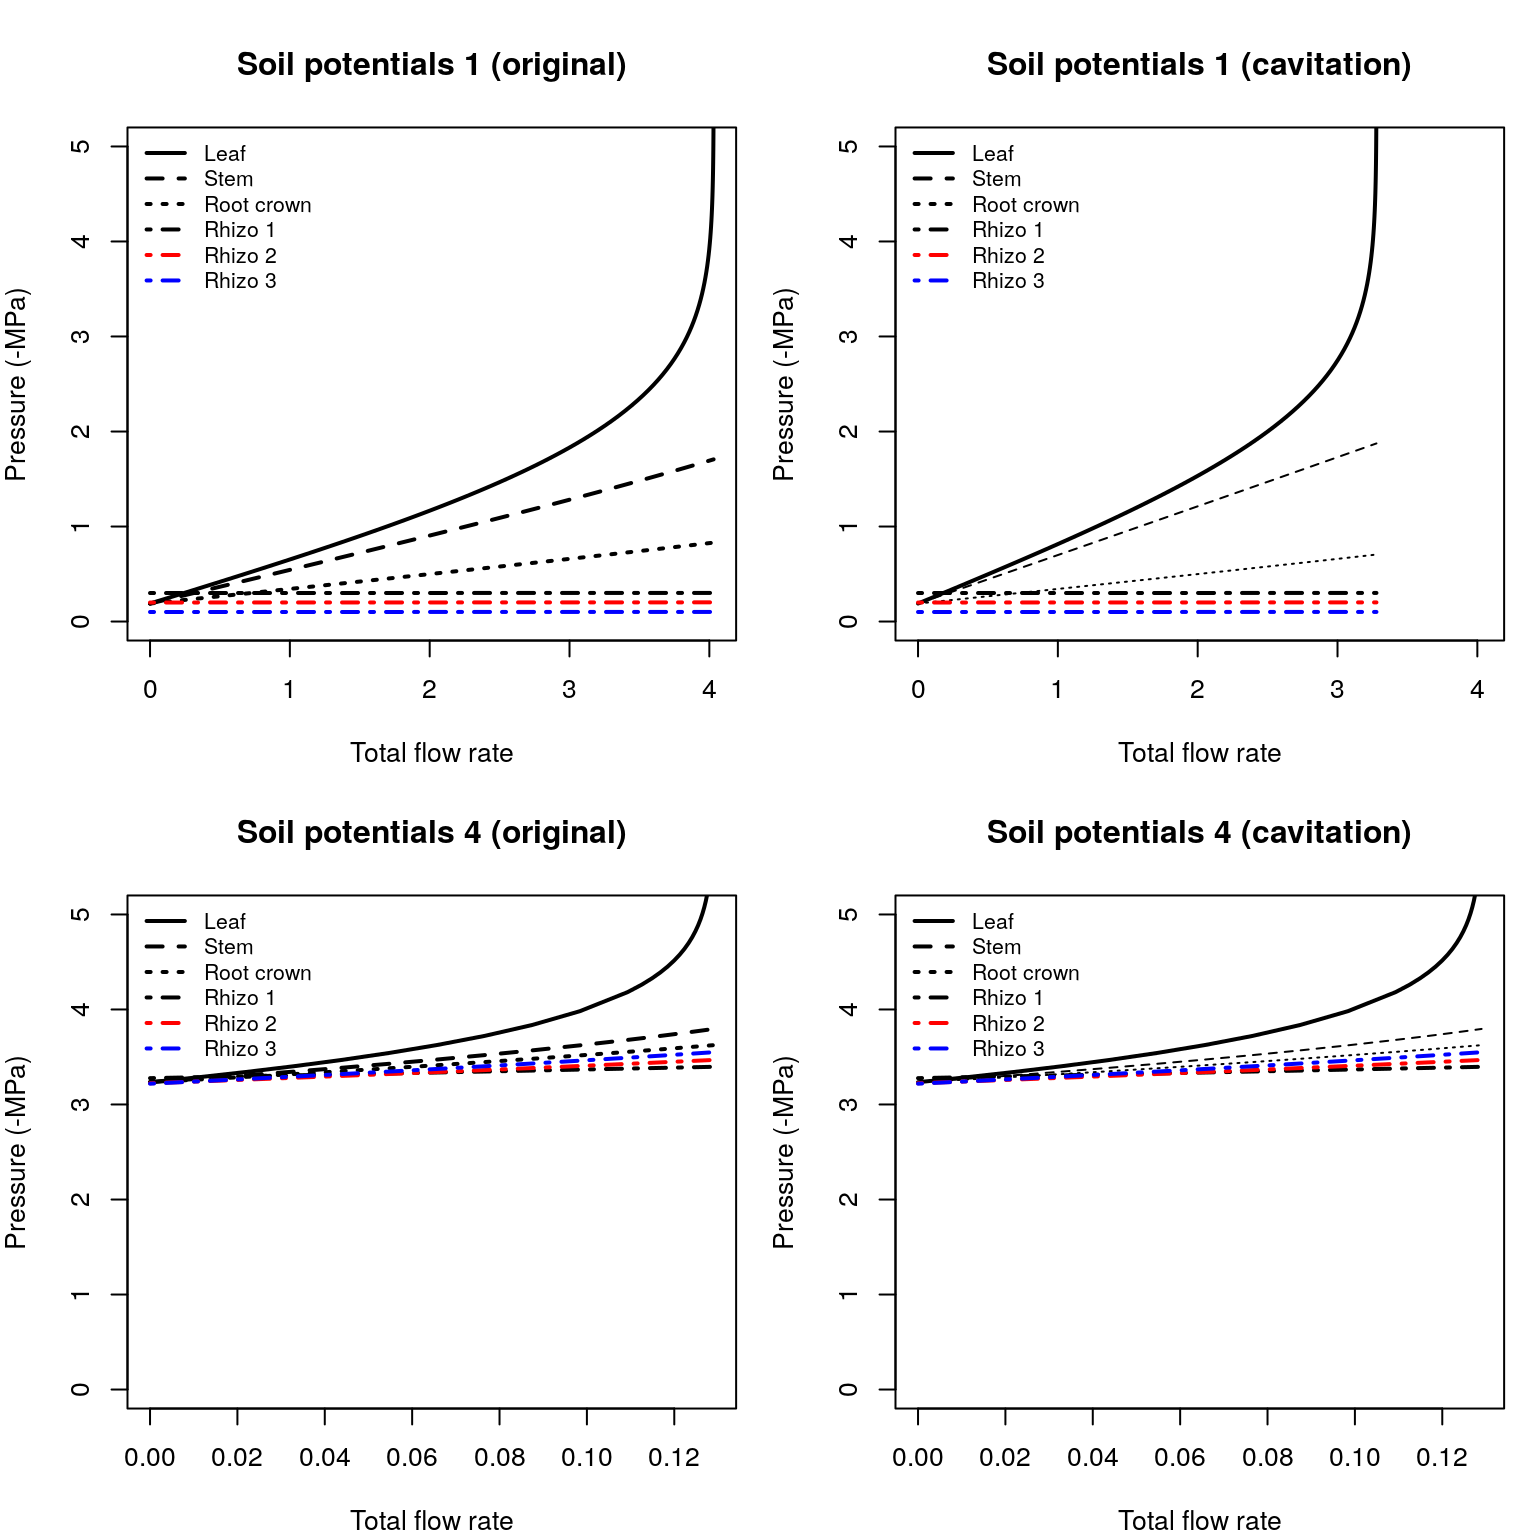
\includegraphics{medfatebook_files/figure-latex/unnamed-chunk-41-1} \end{center}

As with previous representations of the soil-plant continuum, the derivative of \(dE/d\Psi_{leaf}\) for the network topology is obtained numerically:

\begin{center}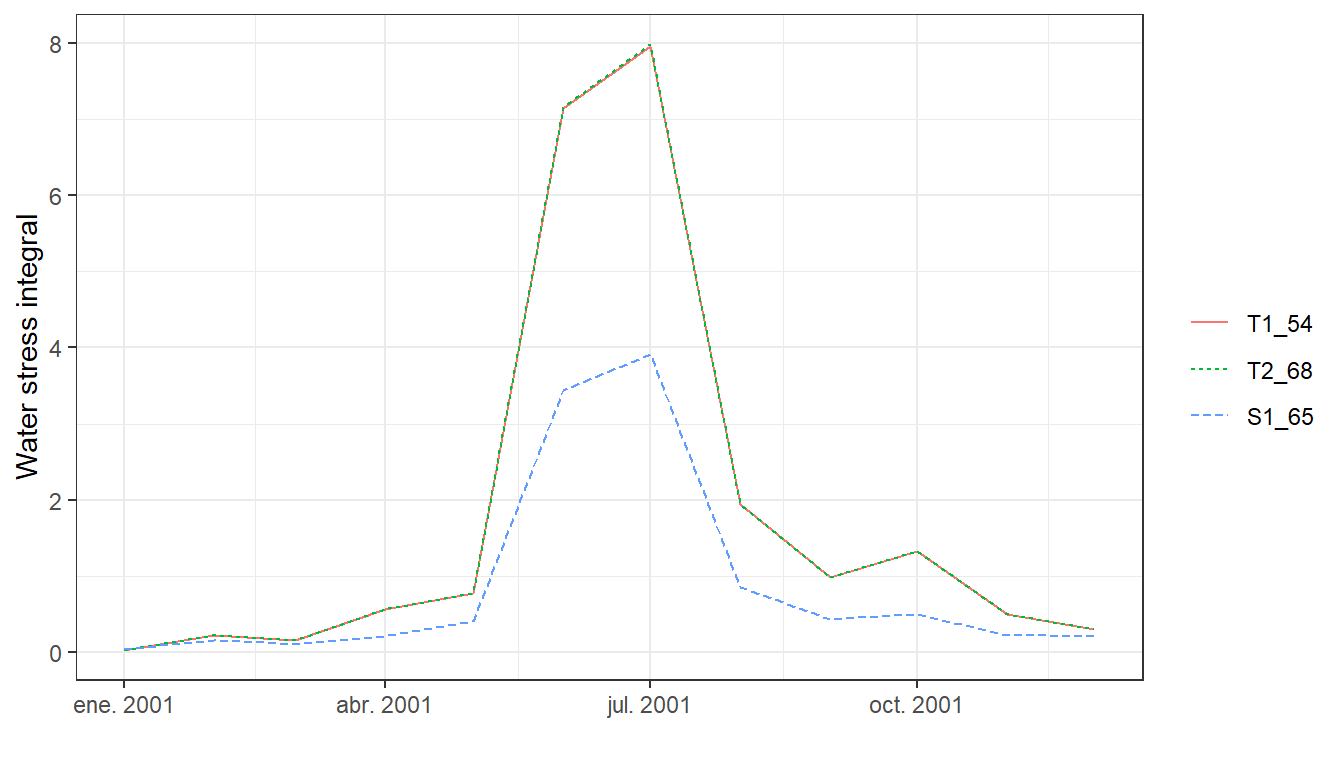
\includegraphics{medfatebook_files/figure-latex/unnamed-chunk-42-1} \end{center}

As with the root system, we can know the water potentials in different points of the continuum. Here we plot them for the results of silt loam texture and the first and last soil potential vectors defined above:

\begin{center}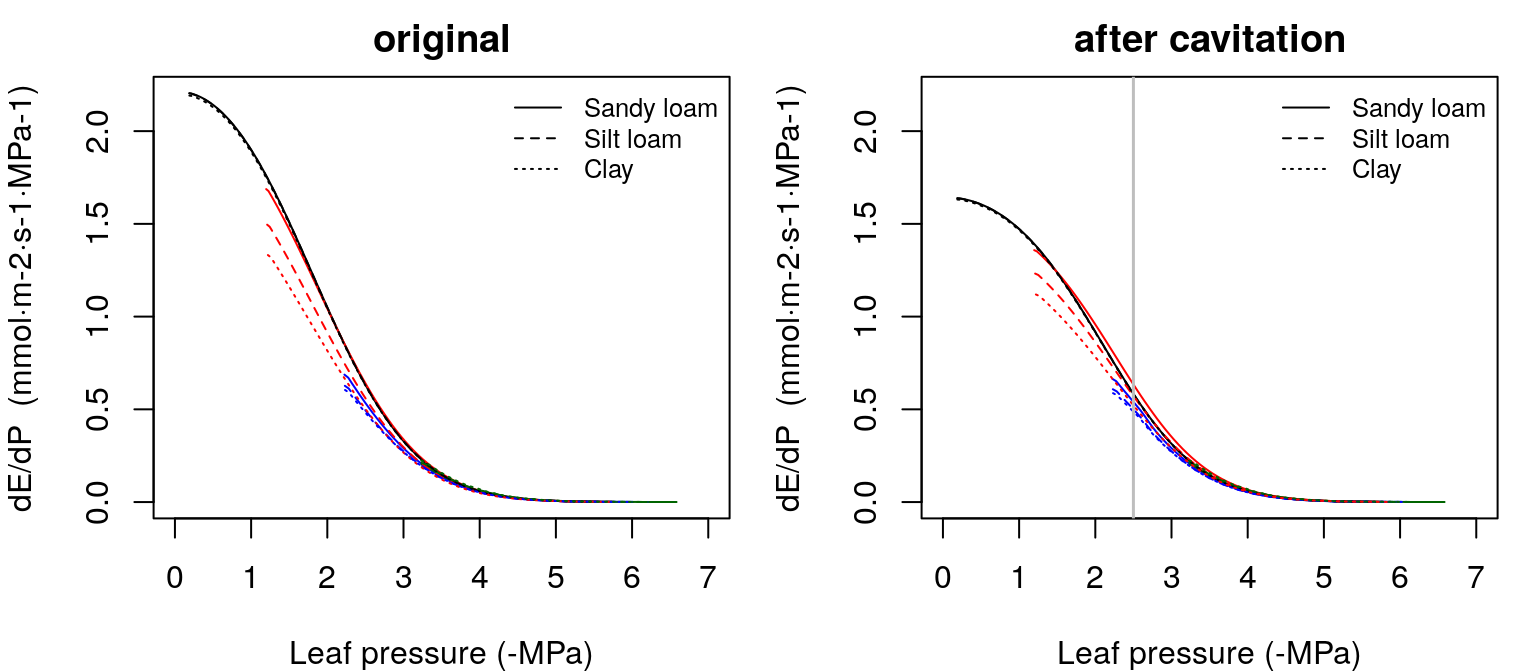
\includegraphics{medfatebook_files/figure-latex/unnamed-chunk-43-1} \end{center}

\hypertarget{supply-function-with-water-compartments}{%
\subsection{Supply function with water compartments}\label{supply-function-with-water-compartments}}

So far we assumed there are no other sources of water than the soil. In this section we consider the effect of additional water from leaf and stem tissues on the supply function. The supply function of a network representing the continuum is build for a given state of soil water potentials. This approach allows determining flows and water potential for \emph{steady-state} conditions. In a dynamic context one has to calculate the supply function for all values of \(E\), then to determine stomatal conductance (see sections devoted to photosynthesis and stomatal regulation) and finally to decide on a specific value of \(E\) and the corresponding steady-state configuration. Because light and temperature conditions change along the day, steady-state stomatal conductance and instantaneous \(E\) values have to be determined for subdaily steps (e.g.~1-hour steps) and then flows need to be scaled and aggregated. At the end of the day, one may substract water from soil layers and recalculate the supply function for the next day.

When considering water compartments, plant transpiration can be larger or smaller than the water extracted from the soil. Moreover, the supply function of a given time step will be dependent on the status of storage comparments in the previous time step, because this determines how much water is added or removed to the stemflow due to the effect of water compartments. For any segment (either a stem segment or the leaf segment) the flow out of it, \(E_{i,out}\), is not necessarily equal to the flow entering the segment, \(E_{i, in}\). Thus, instead of eq. \ref{eq:generalsupply}, the equation governing the flow is (Sperry et al.~1998; Steppe et al.~2005):
\begin{equation}
E_{i,out} = E_{i, in} - \frac{\Delta S_{i}}{\Delta t} = \int_{\Psi_{up}}^{\Psi_{down}}{k_i(\Psi) d\Psi} - \frac{\Delta S_{i}}{\Delta t}
\end{equation}

\begin{figure}

{\centering 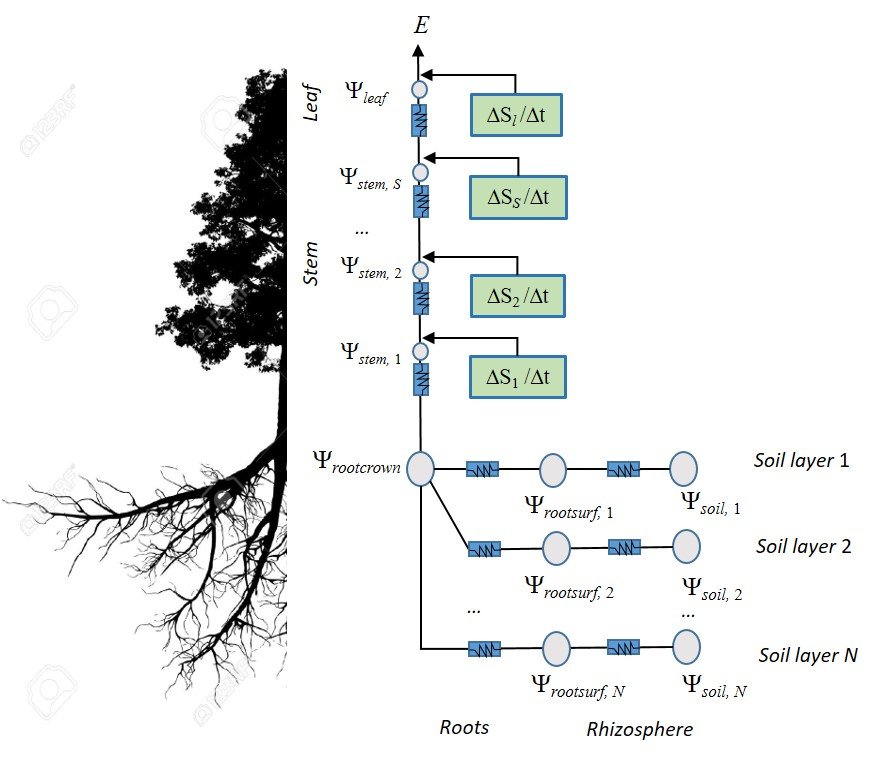
\includegraphics[width=0.8\linewidth]{hydraulics_full} 

}

\caption{Schematic representation of hydraulics in a whole-plant network with water compartments}\label{fig:unnamed-chunk-44}
\end{figure}

When building the supply function from the root crown to the leaf, one has to consider changes in storage water of the current segment before processing the next segment. Specifically, for every segment \(i\) we take the current downstream water potential of the previous segment as upstream water potential (i.e. \(\Psi_{up} = \Psi_{rootcrown, t}\) when processing the first stem segment, \(\Psi_{up} = \Psi_{i-1, t}\) when processing intermediate stem segments or \(\Psi_{up} = \Psi_{S, t}\) when processing the leaf segment). Then we calculate the steady-state drop in water potential (i.e., determine \(\Psi_{down} = \Psi_{i, t}\)) corresponding to the input flow (\(E_{i,in}\)) using the inverse of the integral transform. If stem cavitation has occurred previously then \(\Psi_{cav,i}\) will limit the maximum conductance. To determine \(E_{i,out}\) we calculate the additional instantaneous flow due to changes in storage water volume (\(\Delta S_{i}/\Delta t\)) using:
\begin{equation}
\Delta S_{i} = S_i(\Psi_{i, t}) - S_i(\Psi_{i, t-1})
\end{equation}

As mentioned when describing water content functions, we consider two sources of water in plant segments \citep{Tyree1990}. The amount of water absorbed by or released from the storage compartment will depend on the properties of the apoplastic and symplastic tissues and the fraction of the segment that corresponds to each kind of tissue. For example, let us take the following storage capacities, fractions of apoplastic tissue and parameters of the pressure-volume curves for symplastic tissue.

\begin{Shaded}
\begin{Highlighting}[]
\NormalTok{Vmaxstem =}\StringTok{ }\FloatTok{0.001005046}
\NormalTok{Vmaxleaf =}\StringTok{ }\FloatTok{0.0001327463}
\NormalTok{stemfapo =}\StringTok{ }\FloatTok{0.8}
\NormalTok{leaffapo =}\StringTok{ }\FloatTok{0.15}
\NormalTok{stempi0 =}\StringTok{ }\DecValTok{-2}
\NormalTok{stemeps =}\StringTok{ }\DecValTok{16}
\NormalTok{leafpi0 =}\StringTok{ }\FloatTok{-1.5}
\NormalTok{leafeps =}\StringTok{ }\DecValTok{8}
\end{Highlighting}
\end{Shaded}

The following figures show the change in supply function caused by stem and leaf water compartments, assuming a 1-hr time step and either 0 MPa or -1.5 MPa as previous water potential for all segments (see function \texttt{hydraulics\_supplyFunctionNetworkCapacitance()}):

\begin{center}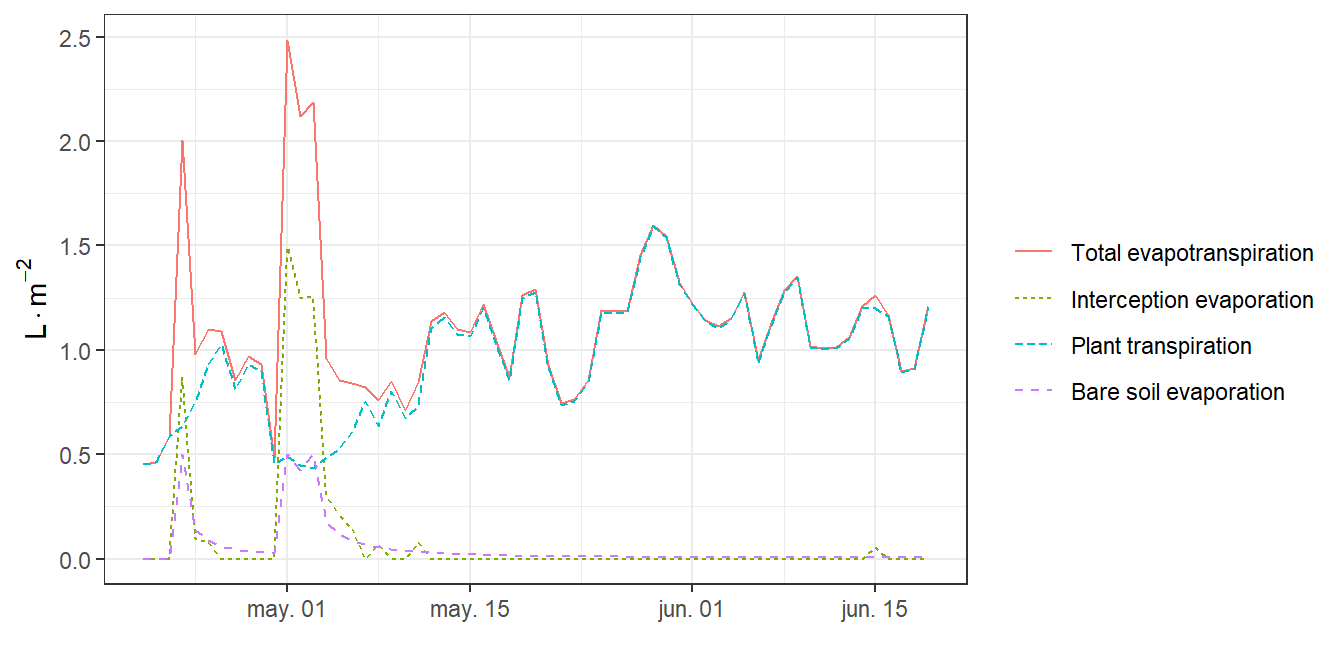
\includegraphics{medfatebook_files/figure-latex/unnamed-chunk-46-1} \end{center}

For the same water potential drop, the effect of the water compartment results in a larger transpiration flow. If the previous water potential is more negative than the root crown, negative flows may occur, because of the need to replenish the water compartment. Note, in addition, that \(dE/d\Psi\) is no longer a non-increasing function of \(\Psi\). This has important consequences for the definition of the cost function (see subsection `Stomatal regulation'). In our opinion, the effect of water compartments on the transpiration flow are important for subdaily variations in transpiration but are less necessary for seasonal to multi-year simulations. However, we will come back to the importance of compartments for plants being disconnected from the soil.

\hypertarget{plant-photosynthesis-and-stomatal-regulation}{%
\chapter{Plant photosynthesis and stomatal regulation}\label{plant-photosynthesis-and-stomatal-regulation}}

\hypertarget{leaf-energy-balance-gas-exchange-and-photosynthesis}{%
\section{Leaf energy balance, gas exchange and photosynthesis}\label{leaf-energy-balance-gas-exchange-and-photosynthesis}}

\hypertarget{leaf-vpd-conductance-to-water-vapor-and-photosynthesis}{%
\subsection{Leaf VPD, conductance to water vapor and photosynthesis}\label{leaf-vpd-conductance-to-water-vapor-and-photosynthesis}}

The water supply function specifies the flow rate, as per leaf area, for values of leaf water potential. If we know air temperature, air vapour pressure and the light conditions in which leaves are, we can be translate the supply function into a photosynthesis function \citep{Sperry2016}. In a nutshell, \(E\) from the supply function is used to calculate leaf temperature from an evaluation of the leaf energy balance. The diffusive conductances of the leaf to water and \(CO_{2}\) are obtained from water supply and water vapor deficit. The gross assimilation rate is then obtained from the diffusive conductance and a modelled curve between assimilation and leaf internal \(CO_{2}\) concentration. Gross assimilation is calculated, without subtracting autotrophic respiration, because the purpose is to represent the instantaneous gain of opening the stomata. Nevertheless autotrophic respiration is included when calculating leaf net photosynthesis.

\begin{Shaded}
\begin{Highlighting}[]
\NormalTok{Tmin =}\StringTok{ }\DecValTok{15}
\NormalTok{Tmax =}\StringTok{ }\DecValTok{30}
\NormalTok{RHmin =}\StringTok{ }\DecValTok{60}
\NormalTok{RHmax =}\StringTok{ }\DecValTok{75}
\NormalTok{Tcan =}\StringTok{ }\NormalTok{meteoland}\OperatorTok{::}\KeywordTok{utils_averageDaylightTemperature}\NormalTok{(Tmin, Tmax)}
\NormalTok{vpa =}\StringTok{ }\NormalTok{meteoland}\OperatorTok{::}\KeywordTok{utils_averageDailyVP}\NormalTok{(Tmin, Tmax, RHmin, RHmax)}
\NormalTok{Patm =}\StringTok{ }\NormalTok{meteoland}\OperatorTok{::}\KeywordTok{utils_atmosphericPressure}\NormalTok{(}\DecValTok{100}\NormalTok{)}

\NormalTok{Q =}\StringTok{ }\DecValTok{2000}
\NormalTok{Catm =}\StringTok{ }\DecValTok{386}

\NormalTok{Vmax298 =}\StringTok{ }\DecValTok{100}
\NormalTok{Jmax298 =}\StringTok{ }\FloatTok{1.67}\OperatorTok{*}\NormalTok{Vmax298}
\NormalTok{Gmin =}\StringTok{ }\FloatTok{0.00001}\NormalTok{;}
\NormalTok{Gmax =}\StringTok{ }\FloatTok{0.3}

\NormalTok{Rabs =}\StringTok{ }\DecValTok{740} \CommentTok{#W * m-2}
\end{Highlighting}
\end{Shaded}

\hypertarget{leaf-temperature-and-vapor-pressure-deficit}{%
\subsection{Leaf temperature and vapor pressure deficit}\label{leaf-temperature-and-vapor-pressure-deficit}}

Leaf temperature (\(T_{leaf}\); in Celsius) can be calculated for any given flow rate \(E(\Psi_{leaf})\) using \citep{Campbell1998}:
\begin{equation}
T_{leaf}(\Psi_{leaf}) = T_{can}+\frac{I_{abs}-\epsilon\cdot\sigma\cdot(T_{can}+273.15)^4-\lambda_v\cdot E(\Psi_{leaf})}{C_p\cdot(g_r+g_{Ha})}
\end{equation}
where \(I_{abs}\) (in \(W \cdot m^{-2}\)) is the instantaneous shortwave and longwave radiation absorbed per leaf area unit, \(E(\Psi_{leaf})\) is the flow (converted to \(mol \cdot s^{-1} \cdot m^{-2}\) per two-sided leaf area basis), \(\epsilon\) is longwave radiation emissivity (0.97), \(\sigma\) is the Stephan-Boltzman constant, \(T_{can}\) is the canopy air temperature (in ºC; see Radiation and energy balance), \(C_p\) = 29.3 \(J \cdot mol^{-1} \cdot ºC^{-1}\) is the specific heat capacity of dry air at constant pressure and \(\lambda_v\) is the latent heat of vaporization (in \(J \cdot mol^{-1}\)):
\begin{equation}
\lambda_v = (2.5023\cdot 10^6-(2430.54\cdot T_{can}))\cdot 0.018
\end{equation}
Finally, \(g_r\) and \(g_{Ha}\) are the radiative and heat conductance values (in \(mol \cdot m^{-2} \cdot s^{-1}\)), respectively \citep{Campbell1998}:
\begin{eqnarray}
g_r &=& \frac{4\cdot \epsilon \cdot \sigma \cdot (T_{can}+273.15)^3}{C_p} \\
g_{Ha} &=& 0.189 \cdot (u/d)^{0.5}
\end{eqnarray}
where \(u\) is wind speed (in \(m \cdot s^{-1}\)), taken as the wind speed at mid-crown height, and \(d\) is 0.72 times the leaf width (species parameter \texttt{LeafWidth} in \(cm\)).

The following figures illustrate the value of \(T_{leaf}\) for two leaf sizes and varying values of wind speed and flow rate, calculated for 24ºC canopy temperature and 740 \(W \cdot m^{-2}\) instantaneous absorved radiation (see function \texttt{biophysics\_leafTemperature}):

\begin{center}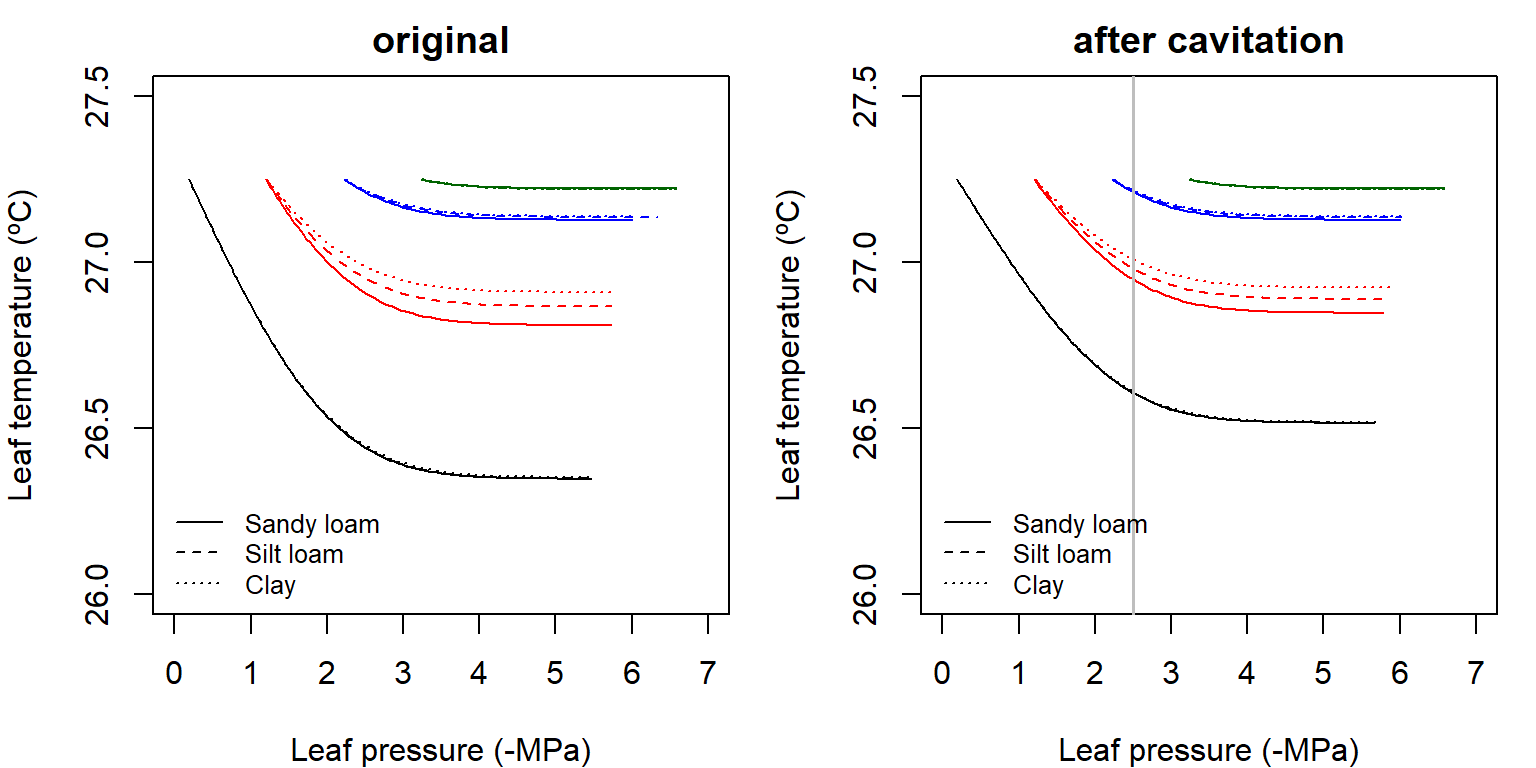
\includegraphics{medfatebook_files/figure-latex/unnamed-chunk-48-1} \end{center}

Let's now fix wind speed to 2 m/s. The application of the above equations to the \(E(\Psi_{leaf})\) curves corresponding to the complete hydraulic network yields the following \(T_{leaf}(\Psi_{leaf})\) curves:

\begin{center}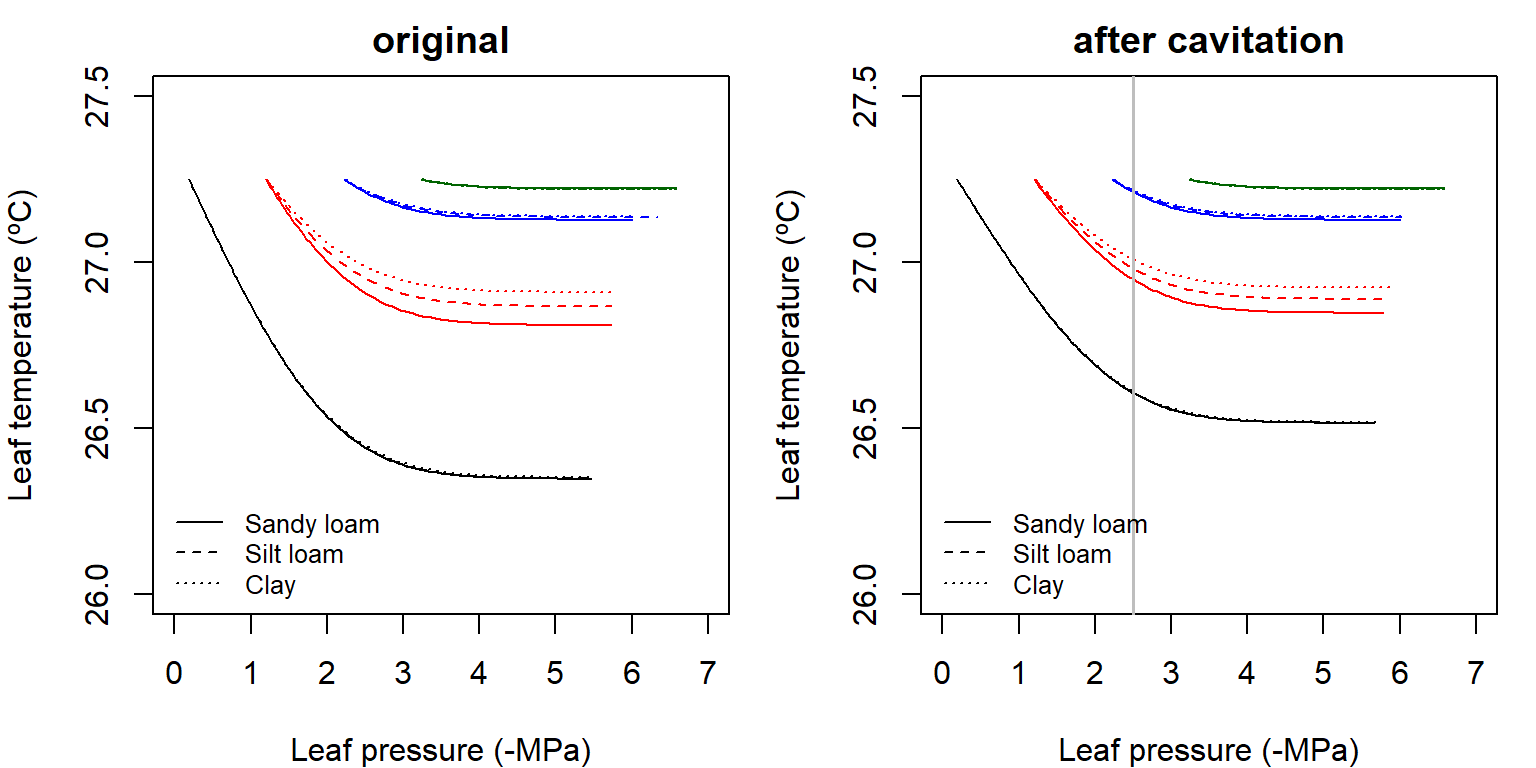
\includegraphics{medfatebook_files/figure-latex/unnamed-chunk-49-1} \end{center}

Thus, transpiration decreases leaf temperature (whereas radiation increases it and wind speed makes it more similar to air temperature). Vapor pressure deficit in the leaf (\(VPD_{leaf}\), in kPa) is calculated as:
\begin{equation}
VPD_{leaf} = VP(T_{leaf})-vp_{day}
\end{equation}
Where \(vp_{day}\) is the average daily vapor pressure and \(VP(T)\) is a function giving the saturated vapor pressure for temperature \(T\). Let us assume the following values of relative humidity, yielding an average \(vp_{day}\):

\begin{Shaded}
\begin{Highlighting}[]
\NormalTok{RHmin =}\StringTok{ }\DecValTok{60}
\NormalTok{RHmax =}\StringTok{ }\DecValTok{75}
\NormalTok{vpa =}\StringTok{ }\KeywordTok{utils_averageDailyVP}\NormalTok{(Tmin, Tmax, RHmin, RHmax)}
\NormalTok{vpa}
\end{Highlighting}
\end{Shaded}

\begin{verbatim}
## [1] 1.912181
\end{verbatim}

the application of the above equation to the \(T_{leaf}(\Psi_{leaf})\) curves yields the following \(VPD_{leaf}(\Psi_{leaf})\) curves:

\begin{center}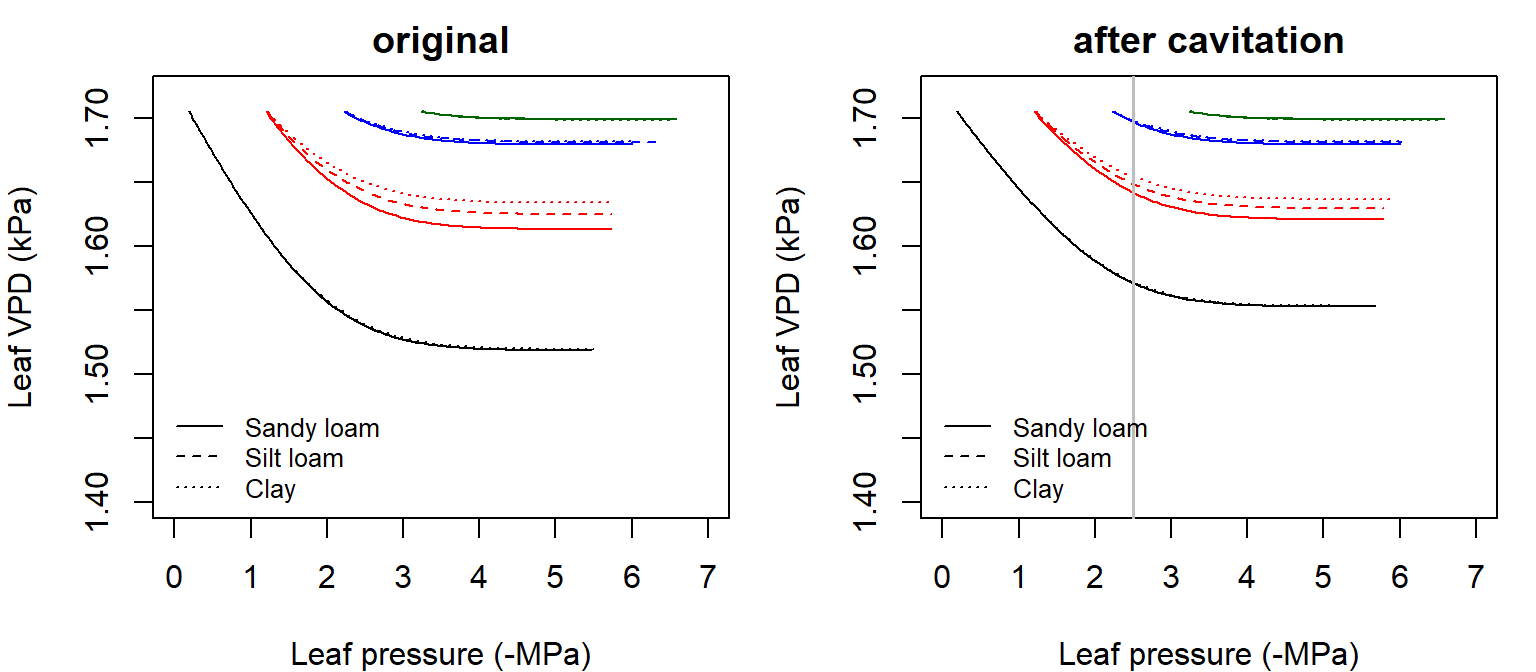
\includegraphics{medfatebook_files/figure-latex/unnamed-chunk-51-1} \end{center}

Since leaf saturated VP decreases when leaf temperature decreases, transpiration decreases leaf VPD as a result of decreasing leaf temperature.

\hypertarget{leaf-conductance-to-water-vapor}{%
\subsection{Leaf conductance to water vapor}\label{leaf-conductance-to-water-vapor}}

Leaf conductance to water vapor (\(g_{sw}\); in \(mol H_2O \cdot s^{-1} \cdot m^{-2}\)) and to carbon dioxide (\(g_{sc}\); in mol \(CO_{2} \cdot s^{-1} \cdot m^{-2}\)) are obtained for each value of \(E\) (in \(mol \cdot s^{-1} \cdot m^{-2}\)) and \(VPD_{leaf}\) using:
\begin{eqnarray}
g_{sw} &=& E \cdot \frac{P_{atm}}{VPD_{leaf}}\\
g_{sc} &=& g_{sw}/1.6
\end{eqnarray}
the application of the equation for \(g_{sw}\) to the \(VPD_{leaf}(\Psi_{leaf})\) curves yields the following \(g_{sw}(\Psi_{leaf})\) curves:

\begin{center}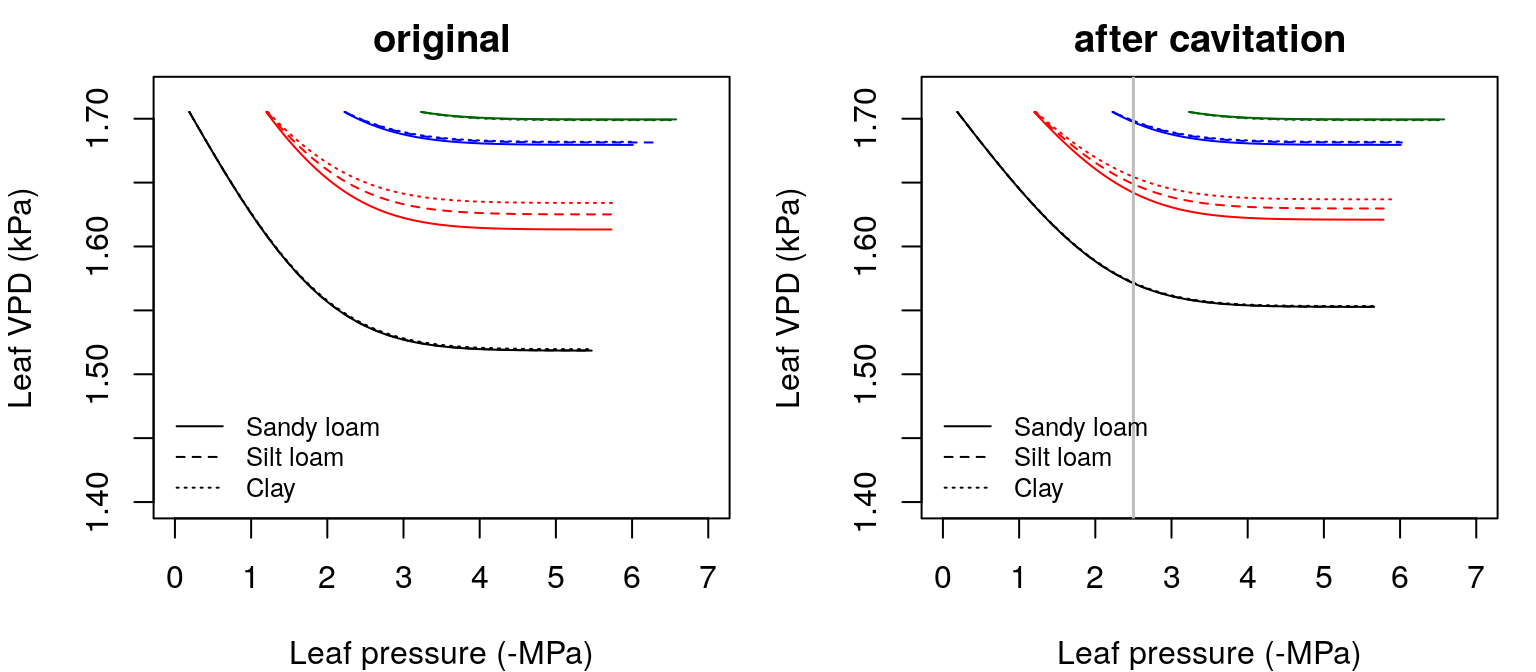
\includegraphics{medfatebook_files/figure-latex/unnamed-chunk-52-1} \end{center}

Hence, larger values of transpiration require larger values of leaf water vapour conductance. In the previous figure we have indicated the thresholds of \(g_{swmin}\) and \(g_{swmax}\), the species-specific minimum and maximum water vapour conductances (i.e.~conductances when stomata are fully closed and fully open, respectively; see parameters \texttt{Gwmin} and \texttt{Gwmax} in \texttt{SpParamsMED}).

\begin{Shaded}
\begin{Highlighting}[]
\NormalTok{Gmin =}\StringTok{ }\FloatTok{0.0045}\NormalTok{;}
\NormalTok{Gmax =}\StringTok{ }\FloatTok{0.3}
\end{Highlighting}
\end{Shaded}

\(g_{sw}\) cannot exceed \(g_{swmax}\) so that some flow rates may not be possible (see stomatal regulation below). However, \(g_{swmax}\) should quickly become non-limiting as soil dries (i.e.~reducing \(E\)) or \(VPD_{leaf}\) increases \citep{Sperry2016}. Minimum stomatal conductance is also used in \textbf{medfate} when building the supply function, as it specifies the minimum flow rates that will occur for completely-closed stomata, i.e.~the minimum flow from which supply function is build.

\hypertarget{leaf-photosynthesis}{%
\subsection{Leaf photosynthesis}\label{leaf-photosynthesis}}

Rubisco-limited photosynthesis rate \(A_c\) (in \(\mu mol CO_2 \cdot s^{-1} \cdot m^{-2}\)) is modelled using \citep{Collatz1991, Medlyn2002}:
\begin{equation}
A_c=\frac{V_{max}\cdot (C_i- \Gamma*)}{C_i+K_c \cdot (1+ O_a/K_o)}
\end{equation}
where \(V_{max}\) is Rubisco's maximum carboxylation rate (in \(\mu mol CO_2 \cdot s^{-1} \cdot m^{-2}\)), \(C_i\) is the internal carbon dioxide concentration (in \(\mu mol \cdot mol^{-1}\)), \(\Gamma*\) is the compensation point (in \(\mu mol \cdot mol^{-1}\)), \(K_c\) (in \(\mu mol \cdot mol^{-1}\)) and \(K_o\) (in \(mmol \cdot mol^{-1}\)) are Michaelis-Menten constants for carboxylation and oxygenation, respectively, and \(O_a\) is the atmospheric oxygen concentration (i.e.~209 \(mmol \cdot mol^{-1}\)). \(\Gamma*\), \(K_c\) and \(K_o\) depend on leaf temperature (\(T_{leaf}\), in Celsius) \citep{Bernacchi2001}:
\begin{eqnarray}
\Gamma* &=& 42.75\cdot e^{\frac{37830\cdot (T_{leaf}-25)}{298\cdot R \cdot (T_{leaf}-273)}}\\
K_c &=& 404.9\cdot e^{\frac{79430\cdot (T_{leaf}-25)}{298\cdot R \cdot (T_{leaf}-273)}}\\
K_o &=& 278.4\cdot e^{\frac{36380\cdot (T_{leaf}-25)}{298\cdot R \cdot (T_{leaf}-273)}}
\end{eqnarray}
Electron transport-limited photosynthesis \(A_e\) (in \(\mu mol CO_2 \cdot s^{-1} \cdot m^{-2}\)) was obtained from \citet{Medlyn2002}:
\begin{eqnarray}
A_e &=& \frac{J}{4}\cdot \frac{C_i-\Gamma*}{C_i+2\cdot \Gamma*} \\
J &=& \frac{(\alpha\cdot Q + J_{max})-\sqrt{(\alpha\cdot Q + J_{max})^2-4.0\cdot c \cdot \alpha \cdot Q \cdot J_{max}}}{2\cdot c}
\end{eqnarray}
where \(\alpha\) is the quantum yield of electron transport (0.3 \(mol electrons \cdot mol photons^{-1}\)), \(Q\) is the PAR photon flux density (\(\mu mol photons \cdot m^{-2} \cdot s^{-1}\)), which is calculated from leaf irradiance (\(I_{par}\); in \(W \cdot m^{-2}\)):
\begin{equation}
Q = I_{par}\cdot 546 \cdot 0.836\cdot 10^{-2}
\end{equation}
\(J_{max}\) and \(J\) are the maximum and actual rate of electron transport (both in \(\mu mol electrons \cdot m^{-2} \cdot s^{-1}\)) and \(c=0.9\) defines the curvature of the light-response curve. The gross assimilation rate \(A\) at a given \(C_i\) is the minimum of \(A_e\) and \(A_c\). To obtain a smooth \(A\)-vs-\(C_i\) curve we used \citep{Collatz1991}:
\begin{equation}
A = \frac{(A_c+A_e)-\sqrt{(A_c+A_e)^2-4.0\cdot c'\cdot A_e\cdot A_c}}{2\cdot c'}
\end{equation}
where \(c'=0.98\) is a curvature factor. The temperature dependence of \(J_{max}\) and \(V_{max}\) relative to 25ºC was modelled using \citet{Leuning2002} (his eq. 1 with parameters from his Table 2). The internal CO\(_2\) concentration, \(C_i\), needs to be known to calculate \(A\) using the previous equations. \citet{Sperry2016a} use a second equation for \(A\) which uses \(g_{cs}\):
\begin{equation}
A = g_{sc} \cdot (C_{atm}-C_i)
\end{equation}
where \(C_{atm}\) is the atmospheric \(CO_{2}\) concentration (in \(\mu mol \cdot mol^{-1}\); see parameter \texttt{Catm} in function \texttt{defaultControl()}). Combining the two equations for \(A\) and finding the root of the resulting equation using Newton-Raphson method allows determining \(C_i\) and therefore \(A\). Thus, after defining PAR photon flux density, atmosphere \(CO_{2}\) concentration and maximum rate parameters:

\begin{Shaded}
\begin{Highlighting}[]
\NormalTok{Q =}\StringTok{ }\DecValTok{2000}
\NormalTok{Catm =}\StringTok{ }\DecValTok{386}
\NormalTok{Vmax298 =}\StringTok{ }\DecValTok{100}
\NormalTok{Jmax298 =}\StringTok{ }\FloatTok{1.67}\OperatorTok{*}\NormalTok{Vmax298}
\end{Highlighting}
\end{Shaded}

one can obtain the following \(A(\Psi_{leaf})\) curves from \(T_{leaf}(\Psi_{leaf})\) and \(g_{sc}(\Psi_{leaf})\):

\begin{center}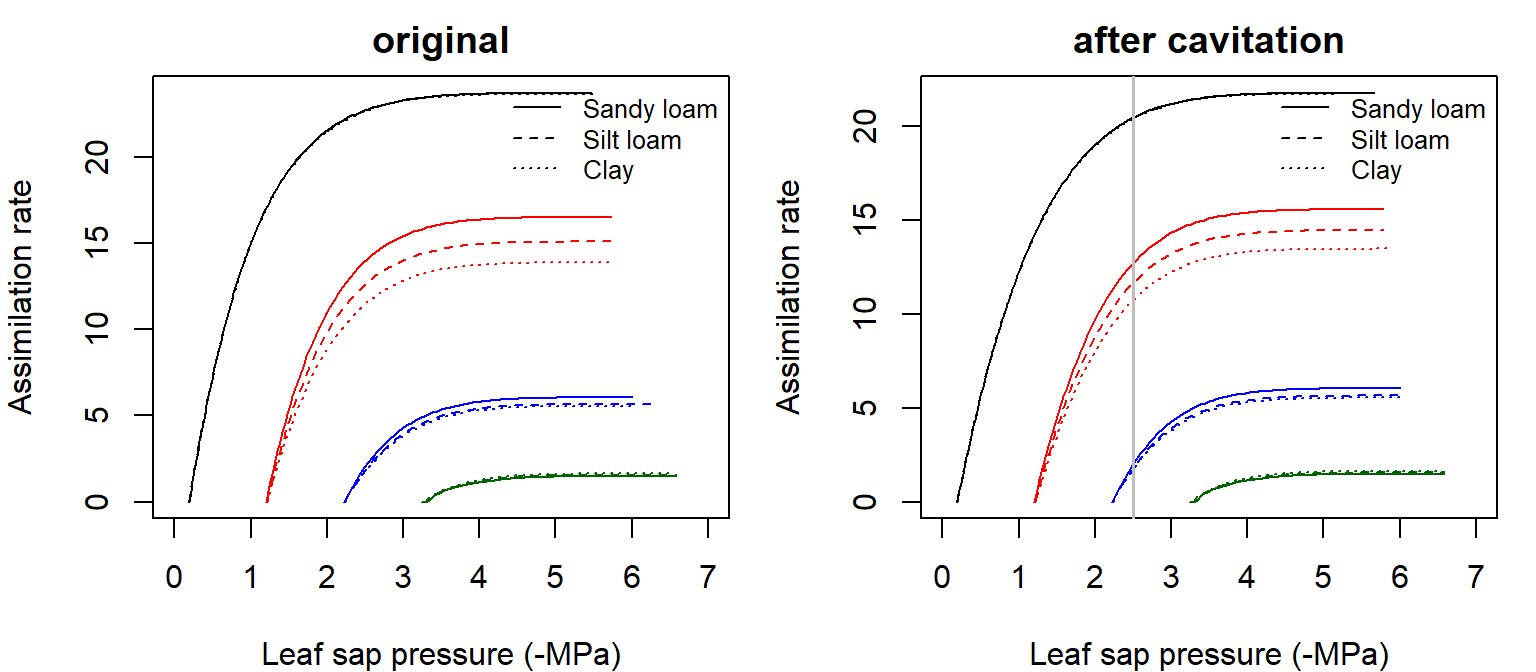
\includegraphics{medfatebook_files/figure-latex/unnamed-chunk-55-1} \end{center}

Finally, leaf net photosynthesis (i.e.~accounting for autotrophic respiration) is calculated as:
\begin{equation}
A_n = A - 0.015 \cdot V_{max}
\end{equation}

\hypertarget{crown-photosynthesis}{%
\section{Crown photosynthesis}\label{crown-photosynthesis}}

In the previous subsection we calculated photosynthesis at the leaf level. However, the function \(A(\Psi_{leaf})\) can be calculated for a whole crown. Essentially we need to repeat the calculations of leaf temperature, leaf VPD, leaf gas conductance and photosynthesis for every leaf to be considered in the crown. Gross and net photosynthesis values can be then aggregated across the crown for each value of \(\Psi_{leaf}\), so that the function \(A(\Psi_{leaf})\) is obtained. Here we will consider a crown of one species divided into 10 layers, with constant leaf density:

\begin{Shaded}
\begin{Highlighting}[]
\NormalTok{LAI =}\StringTok{ }\DecValTok{2}
\NormalTok{nlayer =}\StringTok{ }\DecValTok{10}
\NormalTok{LAIlayerlive =}\StringTok{ }\KeywordTok{matrix}\NormalTok{(}\KeywordTok{rep}\NormalTok{(LAI}\OperatorTok{/}\NormalTok{nlayer,nlayer),nlayer,}\DecValTok{1}\NormalTok{)}
\NormalTok{LAIlayermax =}\StringTok{ }\KeywordTok{matrix}\NormalTok{(}\KeywordTok{rep}\NormalTok{(LAI}\OperatorTok{/}\NormalTok{nlayer,nlayer),nlayer,}\DecValTok{1}\NormalTok{)}
\NormalTok{LAIlayerdead =}\StringTok{ }\KeywordTok{matrix}\NormalTok{(}\DecValTok{0}\NormalTok{,nlayer,}\DecValTok{1}\NormalTok{)}
\NormalTok{kb =}\StringTok{ }\FloatTok{0.8}
\NormalTok{kd_PAR =}\StringTok{ }\FloatTok{0.5}
\NormalTok{kd_SWR =}\StringTok{ }\NormalTok{kd_PAR}\OperatorTok{/}\FloatTok{1.35}
\NormalTok{alpha_PAR =}\StringTok{ }\FloatTok{0.9}
\NormalTok{gamma_PAR =}\StringTok{ }\FloatTok{0.04}
\NormalTok{gamma_SWR =}\StringTok{ }\FloatTok{0.05}
\NormalTok{alpha_SWR =}\StringTok{ }\FloatTok{0.7}
\end{Highlighting}
\end{Shaded}

Many aspects may vary across the crown, including environmental conditions (such as direct/diffuse light or wind speed) and photosynthesis parameters (e.g. \texttt{Vmax298}). The previous crown definition and light parameters lead to a percentage of the above-canopy irradiance reaching each layer \citep{Anten2016}. Furthermore, it is generally accepted that sunlit and shade leaves need to be treated separately \citep{DePury1997}.Extinction of direct radiation also defines the proportion of leaves of each layer that are affected by direct light beams (i.e.~the proportion of sunlit leaves).

\begin{center}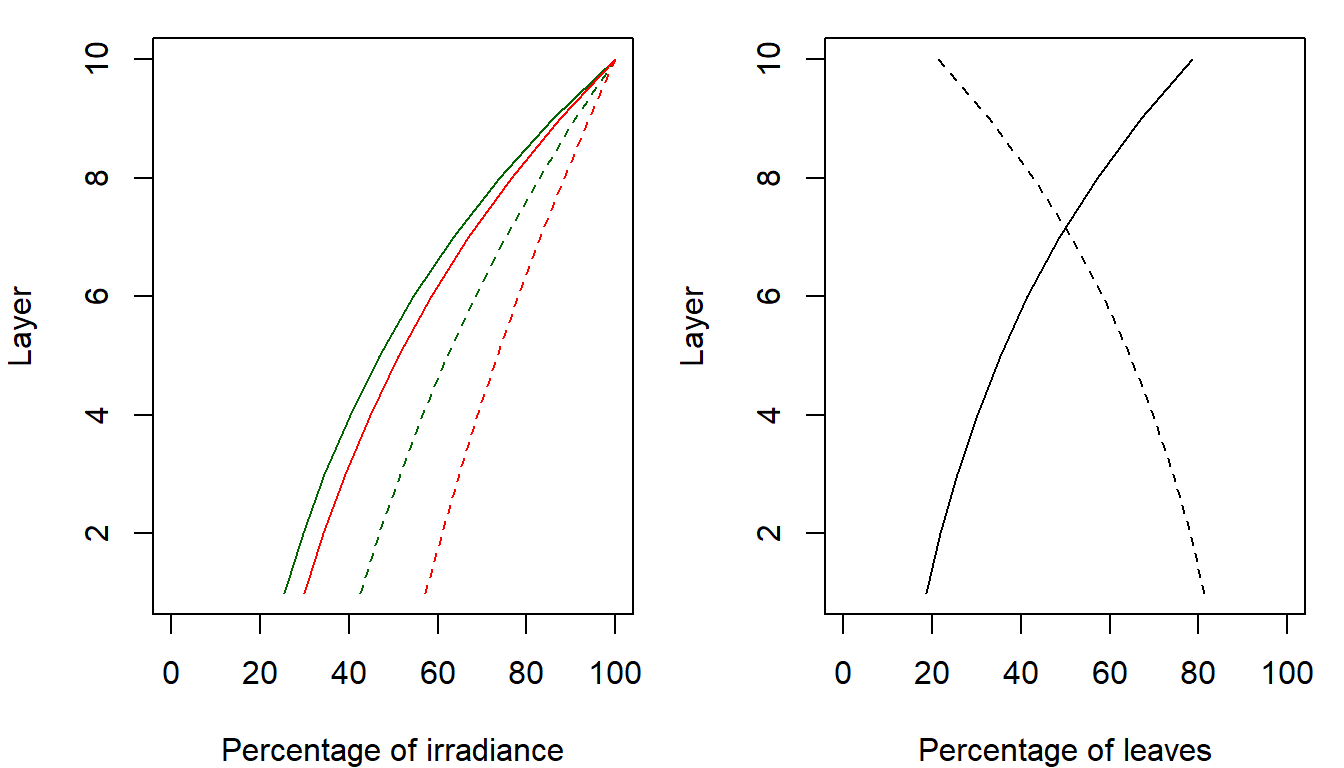
\includegraphics{medfatebook_files/figure-latex/unnamed-chunk-57-1} \end{center}

For simplicity, here we will assume constant windspeed in all layers:

\begin{Shaded}
\begin{Highlighting}[]
\NormalTok{ulayer =}\StringTok{ }\KeywordTok{rep}\NormalTok{(}\DecValTok{2}\NormalTok{, }\DecValTok{10}\NormalTok{)}
\end{Highlighting}
\end{Shaded}

Regarding incoming light, we assume the following direct and diffuse irradiance at the top of the canopy:

\begin{Shaded}
\begin{Highlighting}[]
\NormalTok{solarElevation =}\StringTok{ }\FloatTok{0.67}
\NormalTok{SWR_direct =}\StringTok{ }\DecValTok{1100}
\NormalTok{SWR_diffuse =}\StringTok{ }\DecValTok{300}
\NormalTok{PAR_direct =}\StringTok{ }\DecValTok{550}
\NormalTok{PAR_diffuse =}\StringTok{ }\DecValTok{150}
\end{Highlighting}
\end{Shaded}

Solar elevation is the angle between the sun and the horizon (i.e.~the complement of the zenith angle). Under these conditions, the amount of shortwave and PAR radiation absorbed per unit of leaf area at each canopy layer is \citep{Anten2016}:

\begin{center}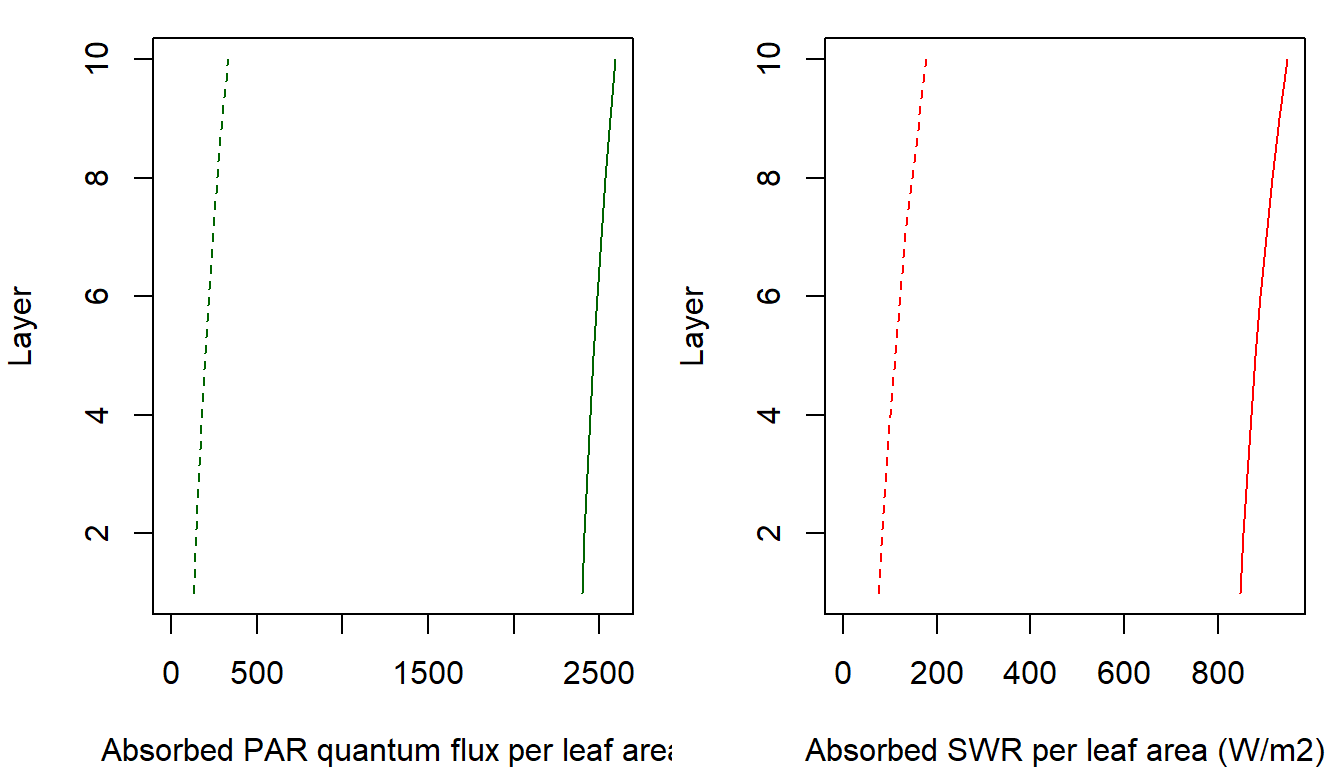
\includegraphics{medfatebook_files/figure-latex/unnamed-chunk-60-1} \end{center}

Following \citet{DePury1997}, we further assume that maximum assimilation rates are highest for leaves at the top of the canopy and there is a exponential decrease from there towards the bottom, where maximum rates are 50\% of those at the top:
\begin{equation}
V_{max,298}(L_i) =V_{max,298}\cdot exp(-0.713\cdot L_i/LAIc)   
\end{equation}
where \(L_i\) is the cumulative LAI value at a given canopy layer \(i\) and \(LAIc\) is the canopy LAI.

Multilayer canopy models allow evaluating leaf conditions, stomatal conductance and photosynthesis for different points of the canopy. However, this comes at high computational cost. While big-leaf canopy models are known to be unaccurate under some situations, sun-shade canopy models \citep{DePury1997} provide estimates that are close to multiple layer models \citep{Hikosaka2016}. Sun-shade models involve: (a) aggregating the leaf area of sunlit/shade leaves across layers; (b) aggregating the light absorbed by leaves of each kind across layers; and (c) aggregating maximum assimilation rates across layers, again separating sunlit and shade leaves. One then calls the photosynthesis model twice (i.e.~once for shade leaves and once for sunlit leaves), using the aggregated maximum assimilation rates. Separating the two kinds of leaves acknowledges that they operate at different parts of the light-saturation curve. The following figure provides the canopy photosynthesis functions obtained, under different situations, using a full 10-layer canopy description (top), a sunshade canopy model (center) or a big-leaf model (bottom). These were generated using functions \texttt{photo\_multilayerPhotosynthesisFunction()}, \texttt{photo\_sunshadePhotosynthesisFunction()} and \texttt{photo\_leafPhotosynthesisFunction()}, respectively. Note the coincidence between the multi-layer and the sun-shade models.

\begin{center}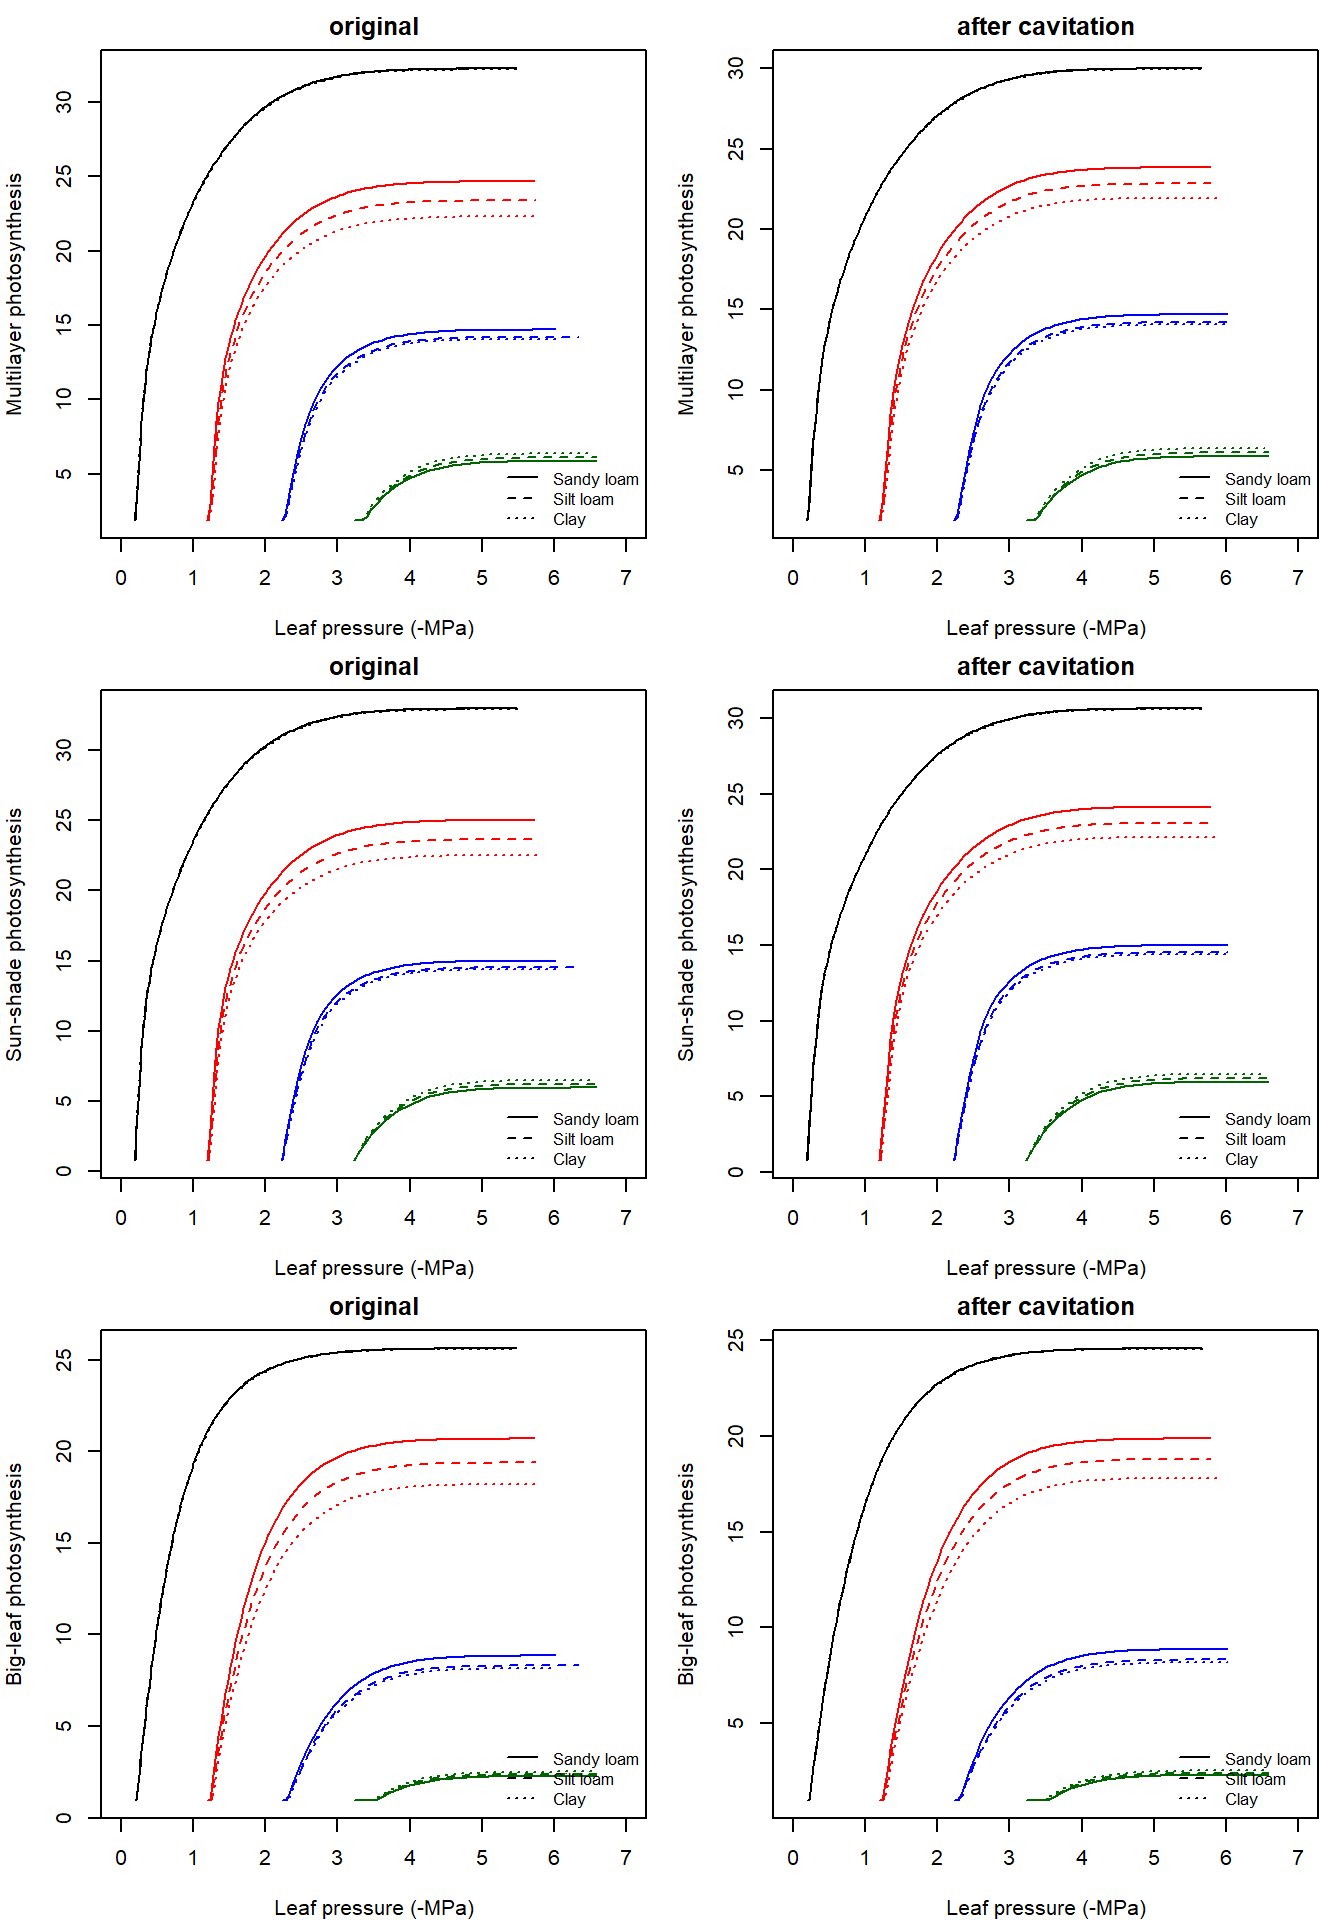
\includegraphics{medfatebook_files/figure-latex/unnamed-chunk-63-1} \end{center}

\hypertarget{stomatal-regulation}{%
\section{Stomatal regulation}\label{stomatal-regulation}}

\citet{Sperry2016} presented a profit maximization approach where hydraulic costs of opening the stomata are compared against photosynthetic gain. Details of their approach, and two suggested variants, a given in the next two subsections. The final subsection explains how to scale stomatal regulation (and hence, transpiration and photosynthesis) from leaf to plant.

\hypertarget{cost-and-gain-functions}{%
\subsection{Cost and gain functions}\label{cost-and-gain-functions}}

The hydraulic supply function is used to derive a transpirational \emph{cost function} \(\theta_1(\Psi_{leaf})\) that reflects the increasing damage from cavitation and the greater difficulty of moving water along the continuum \citep{Sperry2016a}:
\begin{equation}
\theta_1(\Psi_{leaf}) = \frac{k_{c,max}-k_{c}(\Psi_{leaf})}{k_{c,max}-k_{crit}}
\end{equation}
where \(k_c(\Psi_{leaf}) = dE/d\Psi(\Psi_{leaf})\) is the slope of the supply function, \(k_{c,max} = dE/d\Psi(\Psi_{soil})\) and \(k_{crit} = dE/d\Psi(\Psi_{crit})\) is the slope of the supply function at \(E = E_{crit}\) the critical flow beyond which hydraulic failure occurs.

Alternatively, we considered a second cost function (\(\theta_2(\Psi_{leaf})\)) using the vulnerability curve of the leaf:
\begin{eqnarray}
\theta_2(\Psi_{leaf}) &=& \frac{k_{l, max}-k_l(\Psi_{leaf})}{k_{l,max} - k_{l,min}}\\
\end{eqnarray}
where \(k_l\) is the leaf conductance function; and \(k_{l,min}\) and \(k_{l,max}\) are the minimum and maximum leaf conductance values found in the supply function. Using the leaf vulnerability curve for the cost function is grounded on the fact that stomatal regulation occurs at leaves, so that instantaneous regulation should respond to the loss of hydraulic conductance at this point, independently of what happens to the rest of the continuum. Hormonal signals from root to leaf are assumed to regulate stomatal aperture at longer time scales. Obviously, \(\theta_2\) is the same before irreversible cavitation. The difference between them may be interpreted as the following. \(\theta_2\) strictly follows the potential at the leaf level (and hence could be related to a loss of turgor).

The type of cost function can be specified by the user by setting parameter \texttt{hydraulicCostFunction} (see function \texttt{defaultControl()}). The following figures illustrate the \(\theta_1\) and \(\theta_2\) curves corresponding to the supply functions:

\begin{center}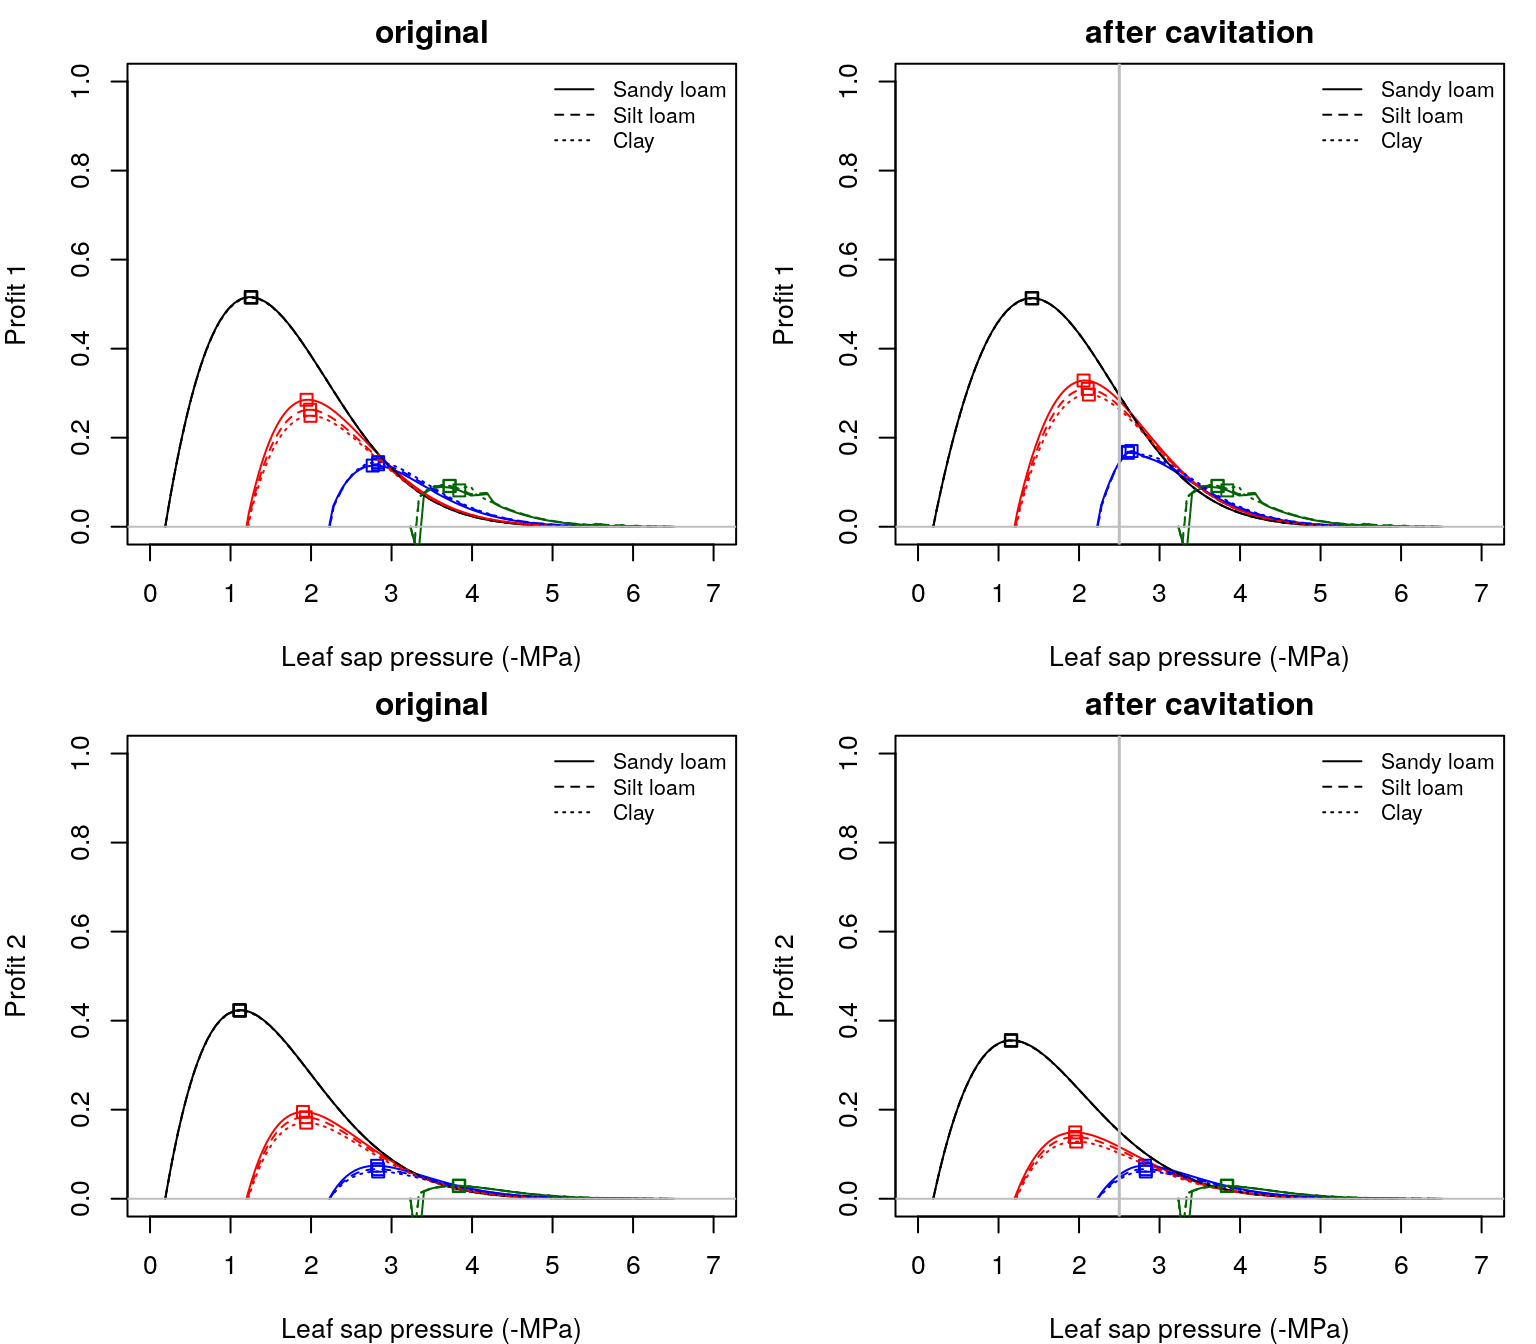
\includegraphics{medfatebook_files/figure-latex/unnamed-chunk-65-1} \end{center}

The normalized photosynthetic \emph{gain function} \(\beta(\Psi_{leaf})\) reflects the actual assimilation rate with respect to the maximum:
\begin{equation}
\beta(\Psi_{leaf}) = \frac{A(\Psi_{leaf})}{A_{max}}
\end{equation}
where \(A_{max}\) is the instantaneous maximum assimilation rate estimated over the full \(\Psi_{leaf}\) range. The following figures illustrate the \(\theta(\Psi_{leaf})\) and \(\beta(\Psi_{leaf})\) curves corresponding to the supply and assimilation functions:

\begin{center}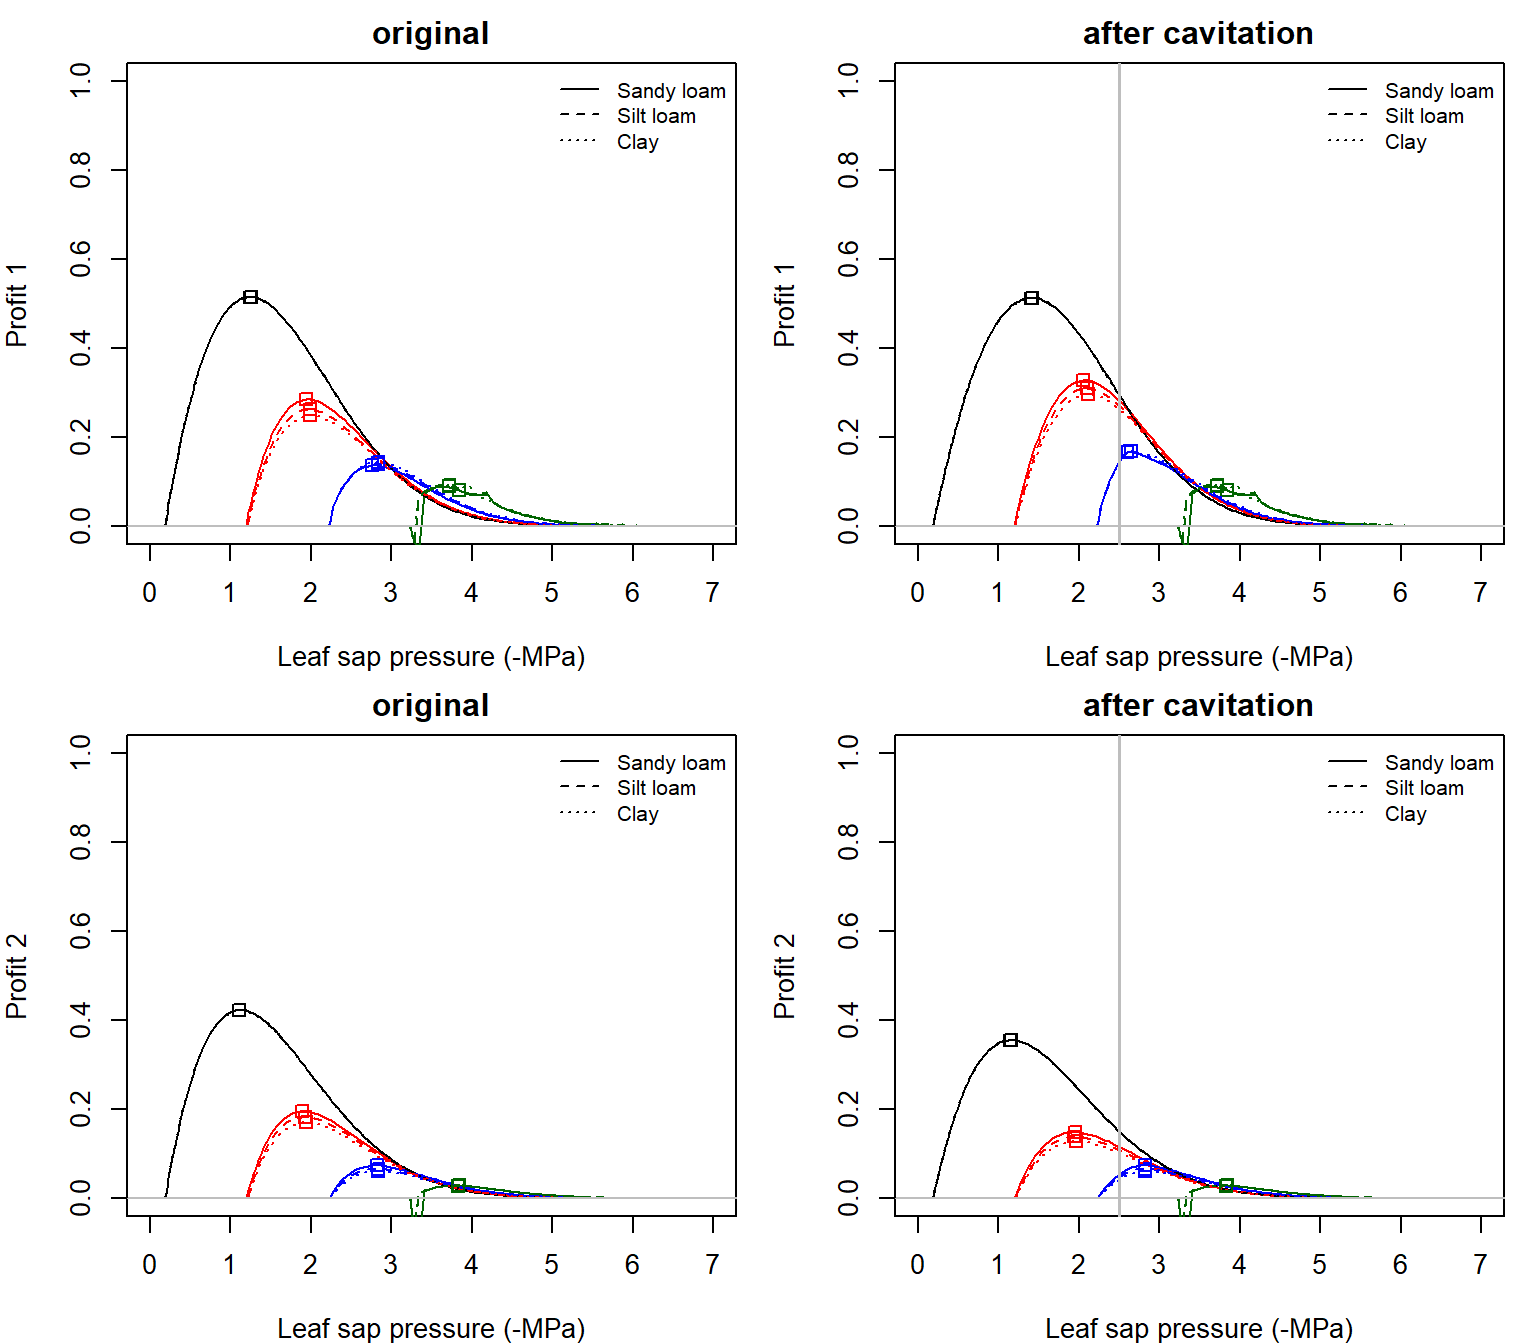
\includegraphics{medfatebook_files/figure-latex/unnamed-chunk-66-1} \end{center}

\hypertarget{profit-maximization-at-the-leaf-level}{%
\subsection{Profit maximization at the leaf level}\label{profit-maximization-at-the-leaf-level}}

According to \citet{Sperry2016}, stomatal regulation can be effectively estimated by determining the maximum of the \emph{profit function} (\(Profit(\Psi_{leaf})\)), for which we consider three alternatives corresponding to the two cost functions:
\begin{eqnarray}
Profit_1(\Psi_{leaf}) &=& \beta(\Psi_{leaf})-\theta_1(\Psi_{leaf})\\
Profit_2(\Psi_{leaf}) &=& \beta(\Psi_{leaf})-\theta_2(\Psi_{leaf})\\
\end{eqnarray}
Once \(\Psi_{leaf}\) that maximizes profit is determined, the values of the remaining variables are also determined. At this point, it may happen that \(g_{sw}(\Psi_{leaf})\) is lower than the minimum (i.e.~cuticular) water vapor conductance (\(g_{swmin}\)) or larger than the maximum water vapor conductance (\(g_{swmax}\)). These thresholds need to be taken into account when determining the maximum of the profit function. The following figures illustrate the \(Profit_1(\Psi_{leaf})\) and \(Profit_2(\Psi_{leaf})\) curves of corresponding to the previous cost and gain curves:
\textbackslash{}begin\{center\}

\begin{center}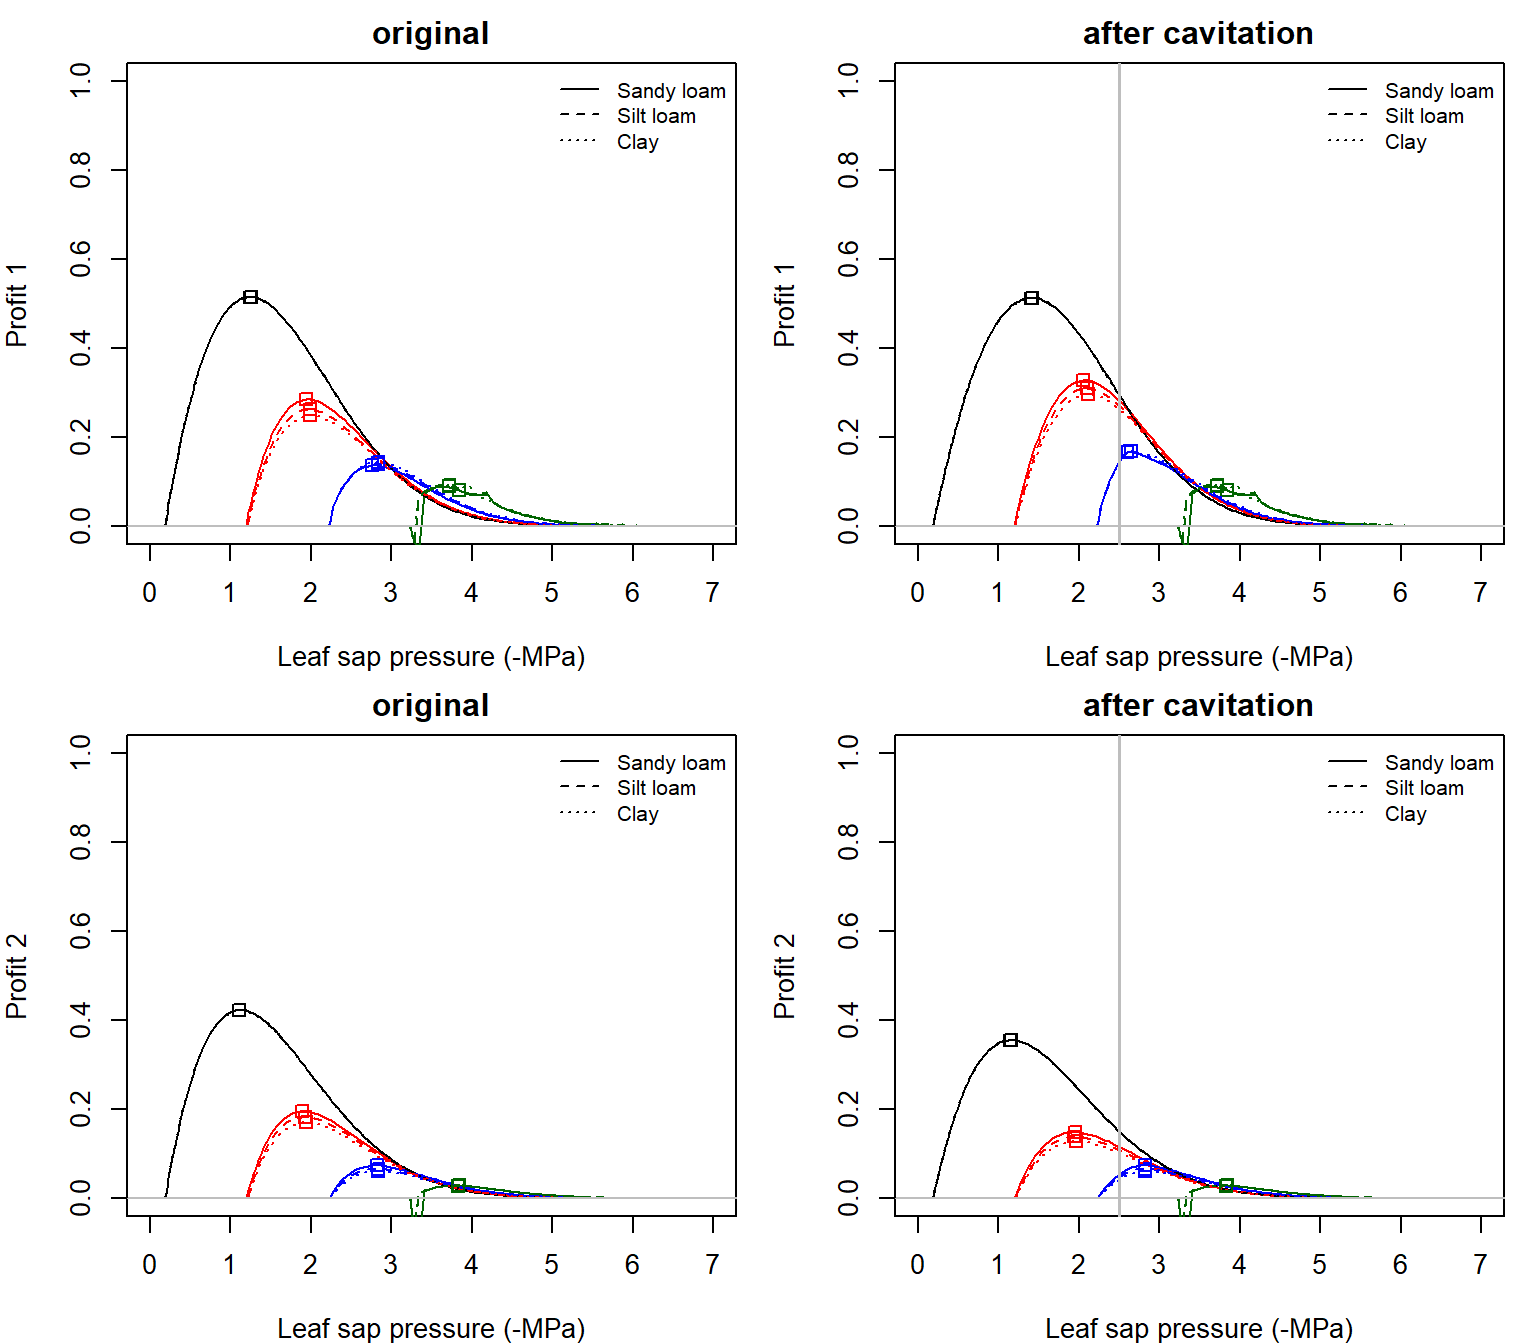
\includegraphics{medfatebook_files/figure-latex/unnamed-chunk-67-1} \end{center}

Squares in the previous figures indicate the maximum profit points in each situation. In the case of non-cavitated system (left panels), the drier the soil, the closer is the maximum profit \(\Psi_{leaf}\) to soil water potential as one would expect intuitively. This occurs for all three profit functions. Unlike \(\theta_1\) which is different for each soil texture (and soil potential), \(\theta_2\) is the same for all soil textures. As a result, the regulation points do not differ much among textures in \(Profit_2\) and \(Profit_3\) because the only difference is in the gain function. For a system with xylem cavitation (right panel), the maximum \(Profit_1\) curves behave strangely. In particular may get a more negative value for \(\Psi_{canopy}\) for wet soils than for dry soils. This effect does not occur when using \(Profit_2\). \(Profit_2\) brings plant water potentials to more negative values after cavitation. Although cavitation did not change the \(\theta_2\) function, the supply function is flatter and this affects the gain function, making it increase less steeply with lower potentials.

Differences between profit functions can be more easily seen when plotting the change from original (uncavitated) regulation to the cavitated one, in terms of both canopy sap pressure and flow rate:

\begin{center}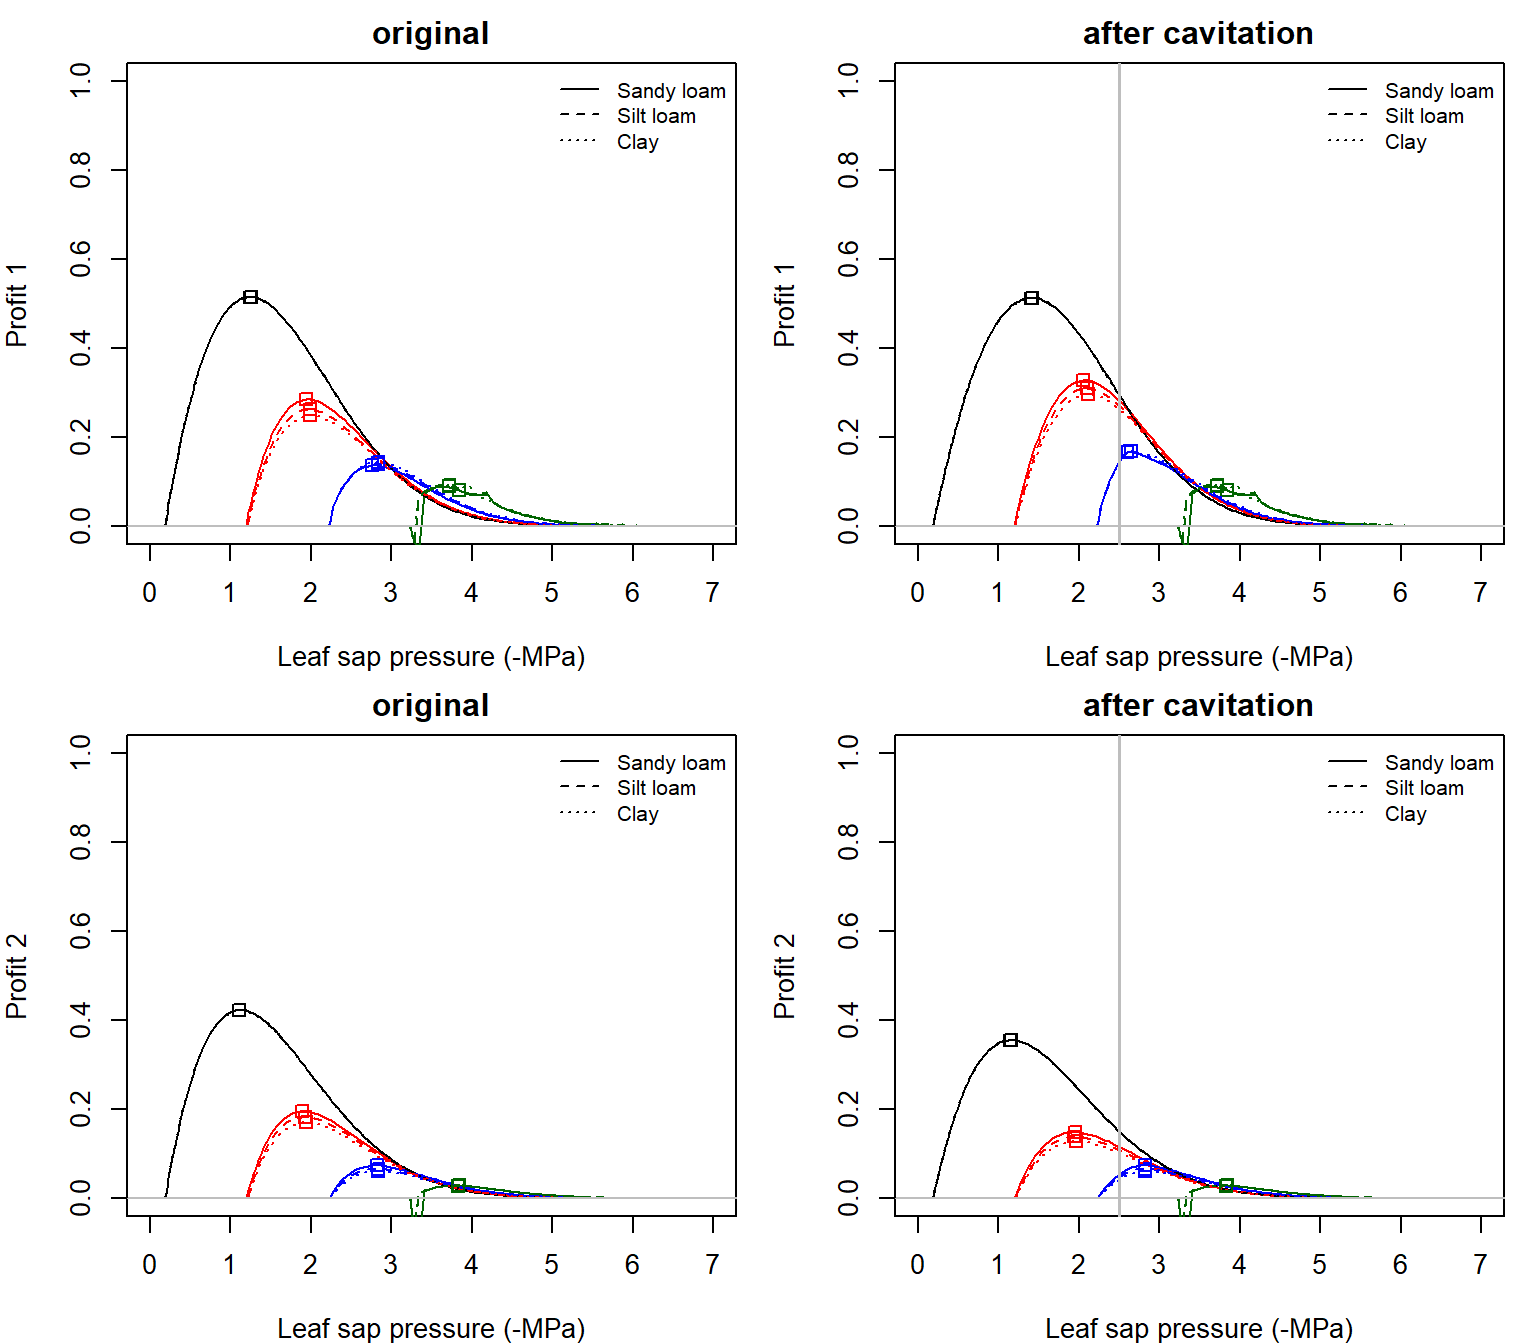
\includegraphics{medfatebook_files/figure-latex/unnamed-chunk-68-1} \end{center}

In \(Profit_1\) irreversible cavitation often brings, after soil rewetting, less conservative stomatal regulation that enables higher flow rates. This does not seem to happen in \(Profit_2\), where despite irreversible cavitation leads to more negative water potentials, predicted flow rates after rewetting are not above those predicted before cavitation.

\hypertarget{scaling-to-the-plant-level}{%
\subsection{Scaling to the plant level}\label{scaling-to-the-plant-level}}

So far, we have considered stomatal regulation by at the leaf level only. At the plant level, the gain function could be build from the crown photosynthesis function \(A(\Psi_{leaf})\) that we defined in subsection `Crown photosynthesis'. However, using the crown photosynthesis function would imply the assumption that the same stomatal aperture occurs in all leaves of the crown, independently of whether they are in shade or sunlit. A more realistic approach is to determine stomatal regulation by profit maximization for sunlit and shade leaves separately; and then determining the average photosynthesis and flow rate from the leaf area of each leaf type. The gain function and profit maximization calculations conducted for each leaf type yield instantaneous water potentials \(\Psi_{sunlit}\) and \(\Psi_{shade}\). They also yield flow values \(E_{shade}\) and \(E_{sunlit}\), in \(mmol H_2O \cdot s^{-1} \cdot m^{-2}\) of leaf area unit. The average flow rate in \(mmol H_2O \cdot s^{-1} \cdot m^{-2}\) per leaf area unit at the plant level is the weighed average:
\begin{equation}
 E_{plant} = \frac{E_{sunlit} \cdot LAI_{sunlit} + E_{shade} \cdot LAI_{shade}}{LAI_{sunlit} + LAI_{shade}}
\end{equation}
where \(LAI_{sunlit}\) and \(LAI_{shade}\) are the cohorts LAI values for sunlit and shade leaves, respectively. Net photosynthesis per leaf area of sunlit and shade leaves (i.e. \(A_{n,sunlit}\) and \(A_{n,shade}\)) is aggregated similarly:
\begin{equation}
 A_{n, plant} = \frac{A_{n,sunlit} \cdot LAI_{sunlit} + A_{n,shade} \cdot LAI_{shade}}{LAI_{sunlit} + LAI_{shade}}
\end{equation}
Profit maximization calculations for shade and sunlit leaves imply different amount of water extracted from the soil layers and different plant water potentials. To overcome this issue, we must use the hydraulic supply function to find the extraction flows from soil layers, the water potential at the root crown and the `average' water potential of the crown all corresponding to the average flow \(E_{plant}\).

\hypertarget{transpirationsperry}{%
\chapter{Transpiration and photosynthesis under Sperry's model}\label{transpirationsperry}}

The model determines transpiration and photosynthesis for each plant cohort separately as follows. First, it updates the hydraulic supply function depending on plant hydraulic characteristics and soil moisture status. Then, transpiration of the plant cohort is estimated for each of them following the framework of \citet{Sperry2016}, who suggest estimating stomatal conductance from the instantaneous maximization of profit, defined as the difference between photosynthesis gain and hydraulic cost (both normalized for comparability). Since the continuum representation implies several soil layers in parallel but joining at the root crown, the hydraulic submodel yields instantaneous water flow and carbon assimilation rates from (or to) each soil layer. Finally, the instantaneous transpiration and assimilation rates of each time step are scaled to the duration of the time step and to the leaf area of the plant cohort. The following provides details for these processes (see further details in Appendices).

\hypertarget{water-supply-function}{%
\section{Water supply function}\label{water-supply-function}}

The supply-loss theory of plant hydraulics of \citet{Sperry2015} uses the physics of flow through soil and xylem to quantify how canopy water supply declines with drought and ceases with hydraulic failure. The theory can be applied to different networks representing the soil-plant continuum, but in our case the continuum is represented using a network of \((N \times 2 + 2)\) resistance elements, with soil being represented in \(N\) different layers. For each soil layer there is a rhizosphere element in series with a root xylem element. The \(N\) different layers are in parallel up to the root crown. From there there is a stem xylem element and a final leaf element.

The \emph{supply function} describes the rate of water supply (i.e.~flow) for transpiration (\(E\)) as a function of the pressure drop between the soil and the leaf, and incorporates both soil, xylem and leaf hydraulic constrains \citep{Sperry1998, Sperry2015, Sperry2016a}. Assuming that maximum conductance values are in mmol \(H_2O \cdot s^{-1} \cdot m^{-2}\) per leaf area unit, transpiration rate (\(E(\Psi_{leaf})\); in mmol \(H_2O \cdot s^{-1} \cdot m^{-2}\) per leaf area unit) is a function of leaf water potential (\(\Psi_{leaf}\); in MPa). The supply function for the whole continuum contains much information. The \(\Psi\) intercept at \(E=0\) represents the predawn canopy sap pressure which integrates the rooted soil moisture profile. As \(E\) increments from zero, the disproportionately greater drop in \(\Psi_{leaf}\) results from the loss of conductance. As the soil dries the differences in flow due to soil texture become more apparent. More details of the calculation of the supply function are given in Appendices.

\hypertarget{leaf-energy-balance}{%
\section{Leaf energy balance}\label{leaf-energy-balance}}

Leaf temperature (\(T_{leaf}\); in Celsius) can be calculated for any given flow rate \(E(\Psi_{leaf})\) using \citep{Campbell1998}:
\begin{equation}
T_{leaf}(\Psi_{leaf}) = T_{can}+\frac{I_{abs}-\epsilon\cdot\sigma\cdot(T_{can}+273.15)^4-\lambda_v\cdot E(\Psi_{leaf})}{C_p\cdot(g_r+g_{Ha})}
\end{equation}
where \(I_{abs}\) (in \(W \cdot m^{-2}\)) is the instantaneous shortwave and longwave radiation absorbed per leaf area unit, \(E(\Psi_{leaf})\) is the flow (converted to \(mol \cdot s^{-1} \cdot m^{-2}\) per two-sided leaf area basis), \(\epsilon\) is longwave radiation emissivity (0.97), \(\sigma\) is the Stephan-Boltzman constant, \(T_{can}\) is the canopy air temperature (in ºC; see `\texttt{Complex model: Radiation and energy balance}'), \(C_p\) = 29.3 \(J \cdot mol^{-1}\cdot ºC^{-1}\) is the specific heat capacity of dry air at constant pressure and \(\lambda_v\) is the latent heat of vaporization (in \(J \cdot mol^{-1}\)):
\begin{equation}
\lambda_v = (2.5023\cdot 10^6-(2430.54\cdot T_{can}))\cdot 0.018
\end{equation}
Finally, \(g_r\) and \(g_{Ha}\) are the radiative and heat conductance values (in \(mol·m^{-2}·s^{-1}\)), respectively (Campbell and Norman 1998):
\begin{eqnarray}
g_r &=& \frac{4\cdot \epsilon \cdot \sigma \cdot (T_{can}+273.15)^3}{C_p} \\
g_{Ha} &=& 0.189 \cdot (u/d)^{0.5}
\end{eqnarray}
where \(u\) is wind speed (in \(m·s^{-1}\)), taken as the wind speed at mid-crown height, and \(d\) is 0.72 times the leaf width (species parameter \texttt{LeafWidth} in \(cm\)).

\hypertarget{leaf-photosynthesis-functions}{%
\section{Leaf photosynthesis functions}\label{leaf-photosynthesis-functions}}

Each water supply value implies an energy balance at the leaf level and a degree of stomatal openness, which ultimately leads to a particular value of leaf photosynthesis. At this point, the model has not decided the amount of water transpired. Therefore, it determines curves depending on leaf water potential for several parameters, as done for \(E(\Psi_{leaf})\). More specifically, for each \(\Psi_{leaf}\) value, the model calculates the corresponding leaf temperature (\(T_{leaf}\); in ºC), leaf-to-air vapor pressure deficit (\(VPD_{leaf}\); in kPa), leaf water vapor conductance (\(g_{sw}\); in \(mol H_2O·s^{-1}·m^{-2}\)) and, finally the leaf gross and net (i.e.~after accounting for autotrophic respiration) photosynthesis assimilation rates (\(A_g\) and \(A_n\); both in \(\mu mol CO_2·s^{-1}·m^{-2}\)). More details of the calculation of these functions are given in Appendices.

Since the model deals with canopies and not single leaves, different parts of the crowns of plant cohorts may be in different canopy positions, which leads to differences in radiation and leaf energy balance. Moreover radiation, energy balance and photosynthesis of leaves vary through the day. Therefore, calculating photosynthesis at the canopy level requires dividing the canopy into \(c\) layers, while differentiating between \textbf{sunlit} and \textbf{shade} leaves. Photosynthesis is calculated by separately for sunlit/shade leaves (De Pury and Farquhar 1997). For each time step, the leaf temperature, leaf VPD and leaf water vapor conductance functions are determined separately for the different leaves.

\hypertarget{stomatal-regulation-1}{%
\section{Stomatal regulation}\label{stomatal-regulation-1}}

Plants must open their stomata to acquire CO\_2 and perform photosynthesis, but doing so promotes water loss. This trade-off has resulted in a tight coordination between capacity to supply and transpire water (hydraulic conductance and diffusive conductance to water vapor) and the maximum capacity for photosynthesis (carboxylation rate and electron-transport rate). For modelling purposes, this carbon-for-water trade-off means that hydraulics, stomatal conductance, transpiration and photosynthesis need to be estimated simultaneously. Here we adopt the framework of \citet{Sperry2016}, who suggest estimating stomatal conductance from the instantaneous maximization of profit, defined as the difference between photosynthesis gain and hydraulic cost (both normalized for comparability).

Stomatal regulation and plant transpiration are determined for each time step separately. The model transforms the slope of the hydraulic supply function into a \textbf{cost function} and the cohort's gross photosynthesis function into a \textbf{gain function}. Then, it finds the \(\Psi_{leaf}\) that maximizes the difference between gain and cost. This simultaneously determines \(E\) and \(A_n\) at the plant cohort level (and also \(T_{leaf}\), \(VPD_{leaf}\), \(g_{sw}\) and \(A_{n}\) for each sunlit/shade leaf in the canopy). The details of all these calculations can be found in Appendices.

While the cost function is the same for the whole day, the gain function and profit maximization calculations are conducted for each of the time steps, yielding instantaneous flow values \(E_{t, s}\) for each soil layer \(s\), in mmol H\(_2\)O·s\(^{-1}\)·m\(^{-2}\) of leaf area unit and instantaneous net assimilation values \(A_{n,t}\) in \(\mu\)mol C·s\(^{-1}\)·m\(^{-2}\) of ground area (i.e.~at the cohort level). To obtain daily values of transpiration at the cohort level the instantaneous flow rates \(E_{t, s}\) need to be scaled to \(E_{step,s}\) using:
\begin{equation}
E_{step,s} = E_{t,s}\cdot 10^{-3} \cdot 0.01802 \cdot LAI_i^{\phi}\cdot \Delta t
\end{equation}
where \$ 0.01802\$ is the molar weight (in kg = L = mm) of water, \(LAI_i^{\phi}\) is the leaf area index of plant cohort \(i\) and \(\Delta t = \tau_{day}/n_t\), being \(n_t\) the number of time steps. The flow rates \(E_{step,s}\) of all steps are added to yield \(E_s\) (in mm H\(_2\)O·day\(^{-1}\)):
\begin{equation}
E_{s} = \sum_{n=1}^{n_t} {E_{step,s}}
\end{equation}
and substracted from the water content of the corresponding soil layer. Daily values of net carbon assimilation for plant cohorts are obtained similarly. The instantaneous rates \(A_{n, t}\) are scaled to \(A_{n,step}\) using:
\begin{equation}
A_{n,step} = A_{n, t} \cdot 10^{-6} \cdot 12.01017 \cdot \Delta t
\end{equation}
where \(12.01017\) is the molar weight of carbon (in g). \(A_{n, step}\) values of all steps are added to obtain \(A_n\), the daily net assimilation at the cohort level (in g C·m\(^{-2}\)·day\(^{-1}\)):
\begin{equation}
A_{n,step} = \sum_{n=1}^{n_t} {A_{n,step}}
\end{equation}

\hypertarget{plant-drought-stress-and-water-potentials}{%
\section{Plant drought stress and water potentials}\label{plant-drought-stress-and-water-potentials}}

Because the model determines optimum transpiration for each time step, this leads to a daily sequence of leaf water potential (\(\Psi_{leaf,t}\)) and root crown water potential (\(\Psi_{rootcrown,t}\)) values. The model chooses as the leaf water potential of the day for cohort \(i\) (\(\Psi_{leaf,i}\)) the minimum of \(\Psi_{leaf,t}\) values. Analogously, the model chooses as the root crown water potential of the day for cohort \(i\) (\(\Psi_{rootcrown,i}\)) the minimum of \(\Psi_{rootcrown,t}\) values. They represent water potential values that would occur at mid-day. Unlike under the simple transpiration mode, here there is no need to average water potentials under the Sperry transpiration mode, because the differences in potential of soil layers are already integrated in the hydraulic supply function.

In order to have an estimate of daily drought stress for the plant cohort, the model uses the stem vulnerability curve of the plant to find the conductance relative to maximum stem conductance and turns it into its complement:

\begin{equation}
DDS_i = \phi_i \cdot \left( 1.0 - \frac{k_{stem, i}(\Psi_{rootcrown,i})}{k_{\max stem, i}}\right) = \phi_i \cdot \left(1.0 - e^{-(\Psi_{rootcrown,i}/d_{stem})^{c_{stem}}}\right)
\end{equation}

where \(\phi_i\) is the leaf phenological status. Note the use of \(\Psi_{rootcrown,i}\) (and not \(\Psi_{leaf,i}\)) to determine drought stress index. Thus the model tracks the degree of conductance decrease at the beginning of the stem as a measure of drought stress. This choice makes daily drought stress values of the Simple and Complex transpiration modes more comparable (because leaf mid-day water potentials are usually much more negative than soil water potentials) and is a sensible choice if one wants to run the model in irreversible cavitation mode (see below).

\hypertarget{irreversible-cavitation-and-hydraulic-disconnection-1}{%
\section{Irreversible cavitation and hydraulic disconnection}\label{irreversible-cavitation-and-hydraulic-disconnection-1}}

Like with the `Granier' transpiration mode, the water balance model with `Sperry' transpiration mode is normally run assuming that although soil drought may reduce transpiration, embolized xylem conduits are automatically refilled when soil moisture recovers. When setting \texttt{cavitationRefill = FALSE} the model tracks the maximum value of drought stress as before:
\begin{equation}
P_{embolized,i}= \max \{P_{embolized,i}, DDS_i \}
\end{equation}
However, the way that previous cavitation levels are taken into account differs from the `Simple' transpiration mode. In this mode, the stem xylem vulnerability curve is modified by specifying that the maximum conductance value is reduced and set to \(k_{stem,i} \cdot (1.0 - P_{embolized,i})\). This effectively causes the supply function to reach lower flow values for the same water potential drop (see details in Appendices).

When running the model using the `Complex' transpiration mode plants may be allowed to disconnect from the soil when its potential becomes too negative. Parameter \(P_{rootdisc,i}\) can be used to specify the minimum relative conductance value that the plant will tolerate without disconnecting hydraulically from the soil (in normal simulations \(P_{rootdisc,i} = 0\)). Again, this affects the model in a way slightly different than when running the model in `Simple' transpiration mode. Before building the supply function, the model checks if there are layers where the relative conductance of roots (i.e. \(k_{root, i, s}(\Psi_{s})/k_{\max root, i, s}\)) is lower than \(P_{rootdisc,i}\). Those layers where this happens are not considered in the calculation of the supply function and do not contribute to transpiration or to the determination of plant water potentials.

\hypertarget{transpiration-and-photosynthesis-after-soil-disconnection}{%
\section{Transpiration and photosynthesis after soil disconnection}\label{transpiration-and-photosynthesis-after-soil-disconnection}}

Considering water compartments allows tracking leaf and stem (i.e.~plant) \emph{dessication}, either when the plant is connected to the soil or when transpiration flow comes from the plant itself. In \textbf{medfate}, disconnection from a given soil layer occurs when its water potential is too low with respect to the root xylem vulnerability curve. The user can control this behaviour by specifying a \(p_{root}\) threshold for relative conductance, and the plant will be disconnected from a soil layer if \(k_{r}(\Psi_{soil})/k_{r,max} < p_{root}\). An interesting situation arises when a plant is disconnected from all soil layers. In this case, the steady-state calculations cannot be used to determine flows, so one is forced to use a full discrete time approximation, with compartments and flows indicated in the figure below.

\begin{figure}

{\centering 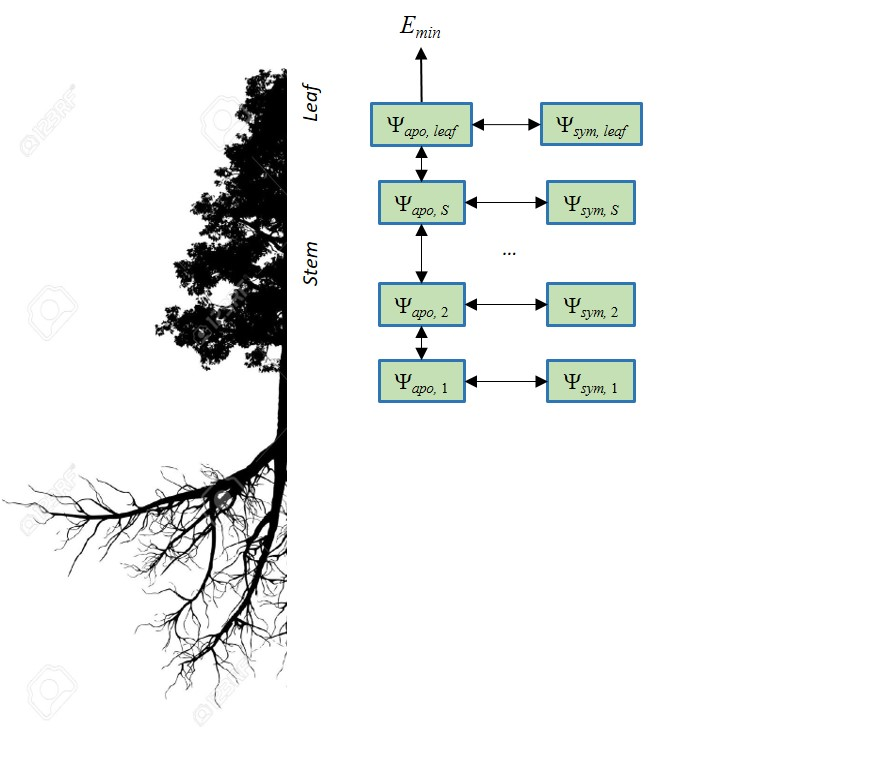
\includegraphics[width=0.8\linewidth]{hydraulics_disc} 

}

\caption{Schematic representation of hydraulics in a whole-plant network after disconnection from soil}\label{fig:unnamed-chunk-69}
\end{figure}

As before, each time step \(\Delta t\) is divided into \(m\) substeps and instantaneous lateral flows between symplastic and apoplastic compartments are calculated as before. In this case, however, one needs to calculate instantaneous flows between stem apoplastic compartments using:
\begin{equation}
F_{i, i+1} = k_{s}(\min(\Psi_{apo,i}, \Psi_{cav, i})) \cdot (\Psi_{apo, i} - \Psi_{apo, i+1})
\end{equation}
and between the last stem compartment and the leaf using:
\begin{equation}
F_{S, l} = k_{l}(\Psi_{apo, l}) \cdot (\Psi_{apo, S} - \Psi_{apo, l})
\end{equation}
The flow from the leaf to the atmosphere is dictated by the minimum stomatal conductance and the vapour pressure deficit. For each time substep all flows are calculated and water content of compartments is updated. Then the equations of relative water content are inversed to find the water potentials for the next time substep.

The instantaneous flow rate between symplastic and apoplastic compartments can be approximated using a lateral conductance \(k_{lat}\) and the difference in water potentials. For the leaf we have:
\begin{equation}
F_{lat, l} = k_{lat} \cdot (\Psi_{sym, l} - \Psi_{apo,l})
\end{equation}
where \(\Psi_{sym, l}\) is the water potential of the symplastic leaf compartment and \(\Psi_{apo,l}\) is the water potential in the apoplastic leaf compartment. If \(\Psi_{sym, l} > \Psi_l\) then the flow will be positive towards the leaf apoplasm and if \(\Psi_{sym, l} < \Psi_l\) the flow will instead refill the leaf symplastic tissue. An analogous equation can be used to calculate the instantaneous lateral flow between symplastic and apoplastic compartments in any stem segment:
\begin{equation}
F_{lat, i} = k_{lat} \cdot (\Psi_{sym, i} - \Psi_{apo, i})
\end{equation}

\hypertarget{part-forest-growth-modelling}{%
\part{Forest growth modelling}\label{part-forest-growth-modelling}}

\hypertarget{forest-growth-model}{%
\chapter{Forest growth model}\label{forest-growth-model}}

\hypertarget{design-principles-2}{%
\section{Design principles}\label{design-principles-2}}

The physical structure of the stand is represented in one (vertical) dimension. Height (or depth) is the only dimension that matters (i.e.~the coordinates of plants are not explicit). The model is cohort-based, meaning that similar plant individuals are represented using a single entity with average properties (e.g.~tree height or diameter) and a density variable is used to scale from individual level to the cohort level. Processes are implemented either at the cohort-level (water balance and photosynthesis) or at the individual level (carbon balance and growth). The model has been designed to be executed on forest inventory plots, but it can be run on other kind of vegetation (e.g.~shrublands or crops) provided vegetation is described using the appropriate variables (i.e.~diameter and height for trees, percent cover and height for shrubs). The model tries to reproduce the physiological processes that modulate leaf area changes and plant growth rates. Nevertheless, since the model does not implement all processes that may affect growth (such as nutrient availability), maximum growth rates and maximum plant sizes are constrained from user inputs, to ensure that model can be more easily calibrated and validated with observations. Consequently, we believe the model is suited to study variations of plant growth derived from environmental conditions and competition for light and water.

Leaf area of each plant cohort is divided between live (wether in resistance buds or unfolded leaves) and dead (standing dead trees). Expanded leaf area corresponds to the portion of live leaf area that is unfolded at any given moment through the leaf phenological cycle. Leaf area density of individuals is considered constant across the crown. Sapwood area of individuals is another important state variable. The Pipe model \citep{Shinozaki1964} is adopted to link increments of leaf area, sapwood area and fine root biomass. Ratios of leaf area to sapwood area (Huber value) can vary within species, due to environmental conditions \citep{Mencuccini1995}. The model assumes a constant, species-specific Huber value, but allows deviations from the pipe model caused by drought-related leaf area reductions.

Water fluxes, soil water balance and plant photosynthesis processes follow the design of the soil water balance model and this part of the model design will not be repeated here. Plant respiration is calculated at the individual level, by estimating the respiration of leaves, stem and fine root compartments. While fine root respiration is proportional to leaf respiration, and hence to expanded leaf area, stem respiration depends on plant size.

Growth is determined taking into account environmental limitations on both source (i.e.~carbon assimilation) and sink (i.e.~carbon investment on plant tissue expansion) \citep{Fatichi2014, Guillemot2015, Korner2015}. With respect to carbon availability for growth, the model offers three alternatives. In the first one, carbon available for growth is simply the daily difference between net photosynthesis and maintenance respiration (i.e.~no carbon storage). The second alternatives involves a single (fast) carbon storage pool that allows decoupling assimilation from growth. Finally, the third alternative involves two carbon storage pools (`fast' and `slow') with a transfer rate between them \citep{Richardson2013, Dietze2014}, which we assume to be regulated by the need to maintain, as much as possible, a minimum amount of carbon in the fast pool (i.e.~for metabolic and osmotic purposes). In the second and third modes, maximum overall C storage capacity is proportional to plant size.

The LPG model \citep{Sitch2003} applies different turnover rates for different tissues, but then tries to satisfy the pipe model \citep{Shinozaki1964} by allocating C where it is more limiting. Instead, we assume that baseline leaf and fine root turnover rates are linearly related to conversion from sapwood to heartwood. Similarly to 3-PG \citep{Landsberg1997} we assume that the turnover rate is smallest for young plants, and it increases up to a maximum value. The model assumes that plants cannot suffer from cavitation if the leaf water potential is large enough for growth to occur (i.e.~if cell turgidity is large enough for cell elongation). Similarly, it also assumes that growth stops before cavitation starts during drought events. When sapwood area reduction occurs, this not only reduces leaf area, but also decreases the amount of fast C reserves available for future growth. Thus it is assumed that parts of the plant are effectively disconnected.

Tree structural variables are updated as in forest gap models \citep{Lindner1997}.

\hypertarget{state-variables-2}{%
\section{State variables}\label{state-variables-2}}

\hypertarget{process-scheduling-2}{%
\section{Process scheduling}\label{process-scheduling-2}}

Every day the growth model first updates the expanded leaf area of living plants according to the phenology of species and the day of the year. Then the model performs soil water balance, transpiration and photosynthesis calculations by calling the soil water balance submodel. After dealing with water fluxes and photosynthesis, the model determines the amount of respiratory biomass, the maximum storage value per individual and maintenance respiration at the individual level. The comparison between photosynthesis and respiration leads to an amount of carbon available for growth (if no carbon pools are considered) or a change in the amount of fast carbon storage pool (if one or two carbon pools are considered). After that, the model determines variations in sapwood area, dead leaf area and live leaf area, which can originate due to conversion from sapwood to heartwood, growth or drought-induced cavitation. If two carbon storage pools are considered, at the end of the day the model determines the direction and amount of carbon transfer between them. Once a year (or by the end of the simulated period) the model translates sapwood area growth into structural variables (i.e., plant height, tree DBH, tree crown ratio and shrub cover).

\hypertarget{water-balance-plant-transpiration-and-photosynthesis}{%
\subsection{Water balance, plant transpiration and photosynthesis}\label{water-balance-plant-transpiration-and-photosynthesis}}

The growth model calls the soil water balance model as a submodel to perform soil water balance and photosynthesis calculations. We only summarize the steps here. The submodel first increases soil moisture due to precipitation, accounting for canopy interception loss, surface runoff and deep drainage. To calculate water losses due to transpiration, the submodel acts differently depending on whether transpiration mode is set to `Granier' or `Sperry'. Generally speaking, though, the submodel determines stomatal conductance of each plant cohort according to the environmental conditions (i.e.~light, leaf temperature, water vapor deficit and soil moisture) and this leads to an estimation of transpiration and net photosynthesis. The submodel then decreases water content due to bare soil evaporation, and plant transpiration, which completes the daily water balance.

Among other outputs, the soil water balance submodel provides values of leaf water potential \(\Psi_{leaf}\) (in MPa) and net photosynthesis calculated at the plant cohort level, \(A_n^{coh}\) (in \(g C · m^{-2} · day^{-1}\)). \(\Psi_{leaf}\) is used in the growth model to modulate drought effects on growth and leaf area losses (see below), whereas \(A_n\) is obviously needed to determine carbon balance and growth. Since carbon balance is calculated at the individual level, \(A_n^{coh}\) needs to be scaled to net photosynthesis per individual (in \(g C · ind^{-1} · day^{-1}\)) using:
\begin{equation}
A_{n}^{ind} = 10000 \cdot A_n^{coh} / N
\end{equation}
where \(N\) is the density of individuals per hectare.

\hypertarget{model-input-2}{%
\section{Model input}\label{model-input-2}}

\hypertarget{vegetation-state-variables-and-parameters}{%
\subsection{Vegetation state variables and parameters}\label{vegetation-state-variables-and-parameters}}

Vegetation in the stand is described using a set of plant cohorts, described in an object of class \texttt{growthInput}. This function assembles all parameters needed for the simulation of a given stand in a single list. Model parameters are grouped by category. Regarding physical aboveground description of the stand, each plant cohort is defined by its species identity (\(SP\); with R name {[}\texttt{SP}{]}). In addition, each cohort needs to be defined regarding the following state variables:

\begin{itemize}
\tightlist
\item
  \(N\) {[}\texttt{N}{]}: The density of individuals (in \(ind · ha^{-1}\)).
\item
  \(DBH\) {[}\texttt{DBH}{]}: Tree diameter at breast height (in cm).
\item
  \(Cover\) {[}\texttt{Cover}{]}: Shrub percent cover (in \%).
\item
  \(H\) {[}\texttt{H}{]}: Total tree or shrub height (in cm).\}
\item
  \(CR\) {[}\texttt{CR}{]}: Crown ratio (i.e.~the ratio between crown length and total height).\}
\item
  \(LAI^{live}\) {[}\texttt{LAI\_live}{]}: Live leaf area index (one-side live leaf area of plants in the cohort per surface area of the stand) (in m\(^2\)·m\(^{-2}\)).\}
\item
  \(LAI^{\phi}\) {[}\texttt{LAI\_expanded}{]}: Expanded leaf area index (one-side expanded leaf area of plants in the cohort per surface area of the stand) (in m\(^2\)·m\(^{-2}\)).\}
\item
  \(LAI^{dead}\) {[}\texttt{LAI\_dead}{]}: Dead leaf area index (one-side dead leaf area of plants in the cohort per surface area of the stand) (in m\(^2\)·m\(^{-2}\)).\}
\item
  \(LAI^{predrought}\) {[}\texttt{LAI\_predrought}{]}: Live leaf area index before the current drought started (one-side dead leaf area of plants in the cohort per surface area of the stand) (in m\(^2\)·m\(^{-2}\)).\}
\item
  \(SA\) {[}\texttt{SA}{]}: Area of functional sapwood per individual (in cm\(^2\)·ind\(^{-1}\)).\}
\item
  \(C_{fast}\) {[}\texttt{fastCstorage}{]}: Amount of C in the fast carbon storage pool (in g C·ind\(^{-1}\)).\}
\item
  \(C_{slow}\) {[}\texttt{slowCstorage}{]}: Amount of C in the slow carbon storage pool (in g C·ind\(^{-1}\)).\}
\end{itemize}

Excepting \(SP\) (species identity) and \(N\) (density), the remaining aboveground state variables are modified during growth simulations. Belowground parameters are the following:

\begin{itemize}
\tightlist
\item
  \(Z\) {[}\texttt{Z}{]}: The rooting depth (in cm).\}
\item
  \(V\) {[}\texttt{V}{]}: A matrix with the proportion of fine roots in each soil layer.\}
\end{itemize}

Additional belowground variables are included if `transpirationMode = ``Complex''\}. These, and the parameters needed for water balance calculations are described in vignette `\textbf{Soil description and root system architecture}'.

The following physiological parameters are needed for growth calculations:

\begin{itemize}
\tightlist
\item
  \(SLA\) {[}\texttt{SLA}{]}: Specific leaf area (m\(^2\)·kg\(^{-1}\)).
\item
  \(Hv\) {[}\texttt{Al2As}{]}: Huber value. Leaf area to sapwood area ratio (in m\(^2\)·m\(^{-2}\)).\}
\item
  \(W_{dens}\) {[}\texttt{WoodDens}{]}: Wood density (at 0\% humidity) (in g·cm\(^{-3}\)).\}
\item
  \(W_{C}\) {[}\texttt{WoodC}{]}: Wood carbon content in relation to dry weight (in g·g\(^{-1}\)).\}
\item
  \(C_{p,\max}\) {[}\texttt{Cstoragepmax}{]}: Maximum storage capacity, expressed as C per total respiratory C (in gC·gC\(^{-1}\)).
\item
  \(RGR_{\max}\) {[}\texttt{RGRmax}{]}: Maximum daily relative growth rate (in sapwood area basis) (in cm\(^2\)·cm\(^{-2}\)).
\end{itemize}

Another set of parameters is needed to transform changes in sapwood area and leaf area to changes in the structural variables such as tree height, tree crown ratio or shrub cover:

\begin{itemize}
\tightlist
\item
  \(H_{\max}\) {[}\texttt{Hmax}{]}: Maximum plant height (in cm).
\item
  \(f_{HD,\min}\), \(f_{HD,\max}\) {[}\texttt{fHDmin\},}fHDmax`{]}: Minimum and maximum values of the height-diameter ratio (in cm·cm\(^{-1}\)).
\item
  \(Z_{\max}\) {[}\texttt{Zmax}{]}: Maximum rooting depth (in mm).
\item
  \(a_{ash}\) {[}\texttt{Aash}{]}: Regression coefficient for the quadratic relationship between shrub height and shrub area.
\item
  \(a_{bsh}\), \(b_{bsh}\) {[}\texttt{Absh}, \texttt{Bbsh}{]}: Allometric coefficients relating crown phytovolume with dry weight of shrub individuals.
\item
  \(CR\) {[}\texttt{cr}{]}: Ratio between crown length and total height (constant value for shrubs).
\item
  \(r_{6.35}\) {[}\texttt{r635}{]}: Ratio between the dry weight of leaves plus branches and the dry weight of leaves alone for branches of 6.35 mm of diameter.
\item
  \(a_{cr}\), \(b_{1cr}\), \(b_{2cr}\), \(b_{3cr}\), \(c_{1cr}\), \(c_{2cr}\) {[}\texttt{B1cr}, \texttt{B2cr}, \texttt{B3cr}, \texttt{C1cr}, \texttt{C2cr}{]}: Regression coefficients used to update the crown ratio of trees.
\item
  \(a_{cw}\), \(b_{cw}\) {[}\texttt{Acw}, \texttt{Bcw}{]}: Regression coefficients used to calculate the crown width of trees (as intermediary step to obtain the crown ratio).
\end{itemize}

\hypertarget{metereological-input-2}{%
\subsection{Metereological input}\label{metereological-input-2}}

Weather input data must include variables calculated at the \textbf{daily} scale. The variables required by function \texttt{growth()} depend on the transpiration mode, similarly to function \texttt{spwb()}. We recommend meteorological input to be generated using package \textbf{meteoland} \citep{DeCaceres2018}.

\hypertarget{model-output-2}{%
\section{Model output}\label{model-output-2}}

\hypertarget{plant-compartments-respiration-and-carbon-balance}{%
\chapter{Plant compartments, respiration and carbon balance}\label{plant-compartments-respiration-and-carbon-balance}}

\hypertarget{biomass-compartments}{%
\section{Biomass compartments}\label{biomass-compartments}}

Biomass of leaves, sapwood and fine roots is needed in the model to estimate respiratory costs (and, if needed, the size of the C storage pools). Respiratory leaf biomass per individual (\(B_{leaf}\); \(g C·ind^{-1}\)) is the result of dividing live expanded leaf area by \(SLA\) (\(kg dry·m^{-2}\)), the specific leaf area coefficient of the species, and multypling by a carbon conversion factor (0.3 \(gC·g dry^{-1}\)):
\begin{equation}
B_{leaf} = 0.3 \cdot 1000 \cdot LA^{\phi} / SLA
\end{equation}
where \(LA^{\phi} = 10000 \cdot LAI^{\phi} / N\) is the expanded leaf area per individual (in m\(^2\)) and factor 1000 is used to convert from kg to g. Hence, only expanded leaf area has respiratory cost (i.e.~winter resistance buds do not) and counts for C storage purposes.

Respiratory sapwood biomass per individual (\(B_{stem}\); \(g C·ind^{-1}\)) represents the sapwood biomass of stems (including trunks and branches) and coarse roots. It is defined as the product of sapwood area (\(SA\); in \(cm^2\)) per individual times the sum of height (\(H\); in cm) and rooting depth (\(Z\); cm), transformed to carbon biomass using species-specific parameters of wood C density (\(W_{dens}\); \(g dry·cm^{-3}\)) and carbon content (\(W_{C}\); \(g C · g dry^{-1}\)):
\begin{equation}
B_{stem} = SA\cdot (H + Z) \cdot W_{dens} \cdot W_{C}
\end{equation}

Finally, the biomass of fine roots per individual (\(B_{root}\); g C·ind\(^{-1}\)) is simply assumed proportional to expanded leaf biomass per individual:
\begin{equation}
B_{root} = B_{leaf}/2.5
\end{equation}
where 2.5 is a ratio between leaf biomass and fine root biomass. Hence, fine-root maintenance respiration costs are also influenced by leaf-phenological status \citep{Sitch2003}.

\hypertarget{maximum-capacity-of-c-pools}{%
\section{Maximum capacity of C pools}\label{maximum-capacity-of-c-pools}}

If carbon pools are considered, their maximum capacity is updated at this point. If there is a single (fast) carbon pool, its maximum storage capacity per individual (\(C_{fast,\max}\); \(g C·ind^{-1}\)) is defined proportional to the total living biomass (i.e., easily accessed C sources like sugars are assumed to be stored in all living parts of the plant):
\begin{equation}
C_{fast,\max} = C_{p,\max} \cdot (B_{leaf} + B_{stem} + B_{root})
\end{equation}
where \(C_{p,\max}\) is the amount of C storage per plant respiratory C weight. If two carbon pools are considered, their maximum capacity is updated assuming that the fast pool corresponds to 5\% of plant respiratory weight, and the slow pool corresponds to the remaining:
\begin{eqnarray}
C_{fast,\max} &=& 0.05 \cdot (B_{leaf} + B_{stem} + B_{root})\\
C_{slow,\max} &=& \max \left(C_{slow,\max},\, (C_{p, \max}-0.05) \cdot (B_{leaf} + B_{stem} + B_{root})\right)
\end{eqnarray}
Note the maximum function for the slow C pool, which ensures that the size of the slow pool will not decrease if there is a decrease in leaf area. Thus, while the slow C pool is still calculated in relation to the total living biomass, it is assumed to be primarily found in long-lasting organs (stem, roots, lignotubers, \ldots{}).

\hypertarget{maintenance-respiration-and-c-balance}{%
\section{Maintenance respiration and C balance}\label{maintenance-respiration-and-c-balance}}

Individual daily maintenance respiration (\(R^{ind}\); in \(g C·ind^{-1}\)) is calculated for each of the three compartments (leaves, alive vascular tissues (stem and coarse roots), and fine roots) (Mouillot et al.~2001). The model uses a \(Q_{10}\) relationship with temperature, which means that for every 10ºC change in temperature there is a \(Q_{10}\) factor change in respiration. Baseline respiration rates (\(r_{leaf}\), \(r_{stem}\) and \(r_{root}\) for leaves, vascular tissues and fine roots, respectively; in \(gC·gC^{-1}\)) are not species-specific and all refer to 20ºC:
\begin{eqnarray}
R_{leaf} &=& B_{leaf} \cdot r_{leaf} \cdot Q_{10}^{(T_{mean}-20)/10} \\
R_{stem} &=& B_{stem} \cdot r_{stem} \cdot Q_{10}^{(T_{mean}-20)/10} \\
R_{root} &=& B_{root} \cdot r_{root} \cdot Q_{10}^{(T_{mean}-20)/10} \\
R^{ind} &=& R_{leaf}+R_{stem}+R_{root}
\end{eqnarray}
where \(T_{mean}\) is the average daily temperature (in ºC). Note that the output of \texttt{growth()} regarding respiration is actually the result of scaling \(R^{ind}\) to the cohort level (\(R^{coh}\) in \(g C · m^{-2} · day^{-1}\)), for comparability with photosynthesis and transpiration:
\begin{equation}
R^{coh} =  R^{ind} \cdot N / 10000
\end{equation}
If no carbon pools are considered, the carbon available for growth is simply the difference between individual's net photosynthesis and maintenance respiration:
\begin{equation}
C_{available} = \max(0,\, A_n^{ind} -  R^{ind})
\end{equation}
whereas if carbon pools are considered, the fast C pool is updated with the result of adding photosynthesis and subtracting respiration; and the resulting pool size sets the amount of C available for growth:
\begin{eqnarray}
C_{fast} &=& \max(0,\,C_{fast} + A_n^{ind} -  R^{ind})\\
C_{available} &=& C_{fast}
\end{eqnarray}

\hypertarget{sapwood-conversion-to-heartwood-embolism-and-growth}{%
\chapter{Sapwood conversion to heartwood, embolism and growth}\label{sapwood-conversion-to-heartwood-embolism-and-growth}}

\hypertarget{sapwood-conversion-to-heartwood-embolism-and-growth-1}{%
\section{Sapwood conversion to heartwood, embolism and growth}\label{sapwood-conversion-to-heartwood-embolism-and-growth-1}}

\citet{Prentice1993} assumed a constant annual rate of 4\% for the conversion from sapwood to heartwood. Similarly, \citet{Sitch2003} assumed a sapwood annual turnover rate of 5\% for all biomes. A reasonable value for maximum daily turnover rate would be (assuming an annual rate 4.5\%):
\begin{equation}
1-0.955^{(1/365)} = 0.0001261398
\end{equation}
The actual proportion of sapwood area that is transformed into heartwood is:
\begin{equation}
p_{heartwood} = \frac{0.0001261398}{1+15\cdot e^{-0.01\cdot H}}
\end{equation}
where 0.01 is a constant causing short plants to have slower turnover rates.

Sapwood turnover is applied at the same rate in evergreen and deciduous species. The amount of sapwood that is converted to heartwood every day, \(\Delta SA_{turnover}\), is thus:
\begin{equation}
\Delta SA_{turnover} = SA \cdot p_{heartwood}
\end{equation}
Before applying either growth or cavitation the model determines the extent to which cell turgor allows growth using a negative exponential function:
\begin{equation}
f_{turgor}(\Psi_{leaf}) = 1 - \left[e^{(\Psi_{leaf}/\Psi_{tlp})-1}\right]^5
\end{equation}
where \(f_{turgor}(\Psi_{leaf})=0\) if \(\Psi_{leaf} > \Psi_{tlp}\). The following figure illustrates the function for \(\Psi_{tlp}=-1.5\) MPa:

\begin{center}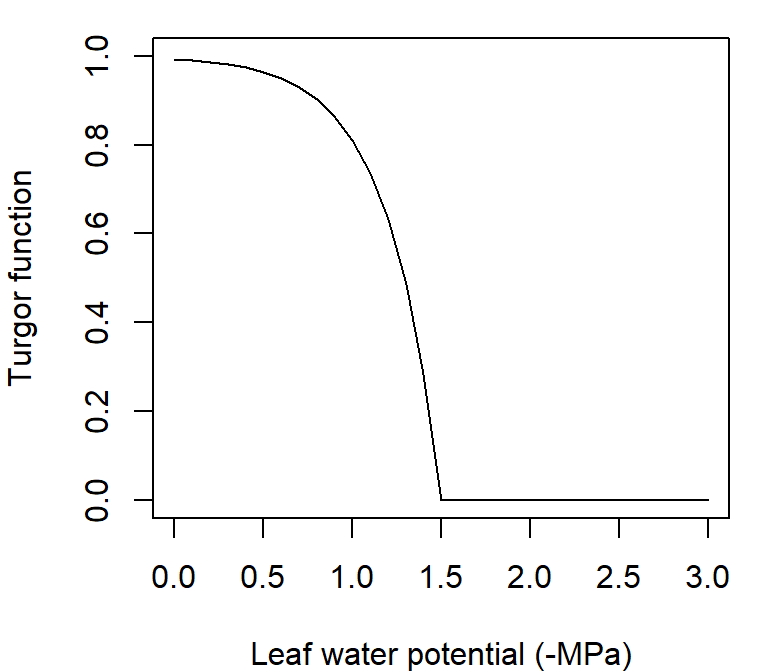
\includegraphics{medfatebook_files/figure-latex/unnamed-chunk-70-1} \end{center}

If \(f_{turgor}(\Psi_{leaf})>0\) growth is applied, but there can be leaf area losses from sapwood turnover, whereas if \(f_{turgor}(\Psi_{leaf}) = 0\) growth does not occur and cavitation is possible. The following two subsection detail the behavior of the growth model in each case.

\hypertarget{growth-and-turnover-during-non-drought-periods}{%
\section{Growth and turnover during non-drought periods}\label{growth-and-turnover-during-non-drought-periods}}

If (i.e.\(f_{turgor}(\Psi_{leaf})>0\)) the model determines growth, expressed as formation of new sapwood and leaf area increase. Daily sapwood growth rate is assumed to depend on the availability of carbon (i.e., \(C_{available}>0\)), but also requires temperature to be within acceptable ranges (because it affects biochemical rates) and minimum turgor for cell elongation.

The adoption of the pipe model (Shinozaki et al.~1964) implies that the addition of new foliage requires building a proportional amount of xylem conduits and fine roots. This is represented in the model by a species-specific Huber value \(Hv\) (in \(m^2·m^{-2}\)). Since all living biomass equations are linearly related to sapwood area, the total cost in g C per 1 \(cm^2\) of newly formed sapwood area:
\begin{eqnarray}
C_{cost,leaf} &=& 0.3 \cdot \frac{0.1\cdot Hv}{SLA}\\
C_{cost,stem} &=& (H + Z) \cdot W_{dens} \cdot W_{C}\\
C_{cost,root} &=& C_{cost,leaf}/2.5\\
C_{cost,overall} &=& 1.3 \cdot (C_{cost,leaf}+C_{cost,stem} + C_{cost,root})
\end{eqnarray}
where 0.1 is needed to express \(C_{cost,leaf}\) in units of \(g · cm^{-2}\) and factor 1.3 is used in the calculation of \(C_{cost,overall}\) because growth respiration is assumed to be a constant proportion of all new tissue growth (30\% of new tissue is respired, Ryan 1990). Note that carbon allocation to the three compartments does not follow constant proportions for different plants because the larger the size of a plant, the more C will need to be allocated in the vascular system per unit of sapwood area increment, and hence the proportion of C allocated to leaves and fine roots will decrease. The maximum increase in sapwood area according to the availability of C is:
\begin{equation}
\Delta SA_{available} = \frac{C_{available}}{C_{cost,overall}}
\end{equation}

Several sink limitations may occur. One is the turgor limitation, which is represented in the model by \(f_{turgor}\). If carbon pools are considered, then the C concentration in the fast pool (i.e. \(C_{fast}/C_{fast, \max}\)) may also limit the rate of growth. We model this sink limitation by assuming that the maximum rate of growth will decrease with decreasing concentration, following a sigmoidal function:
\begin{equation}
f_{conc} = \frac{1}{1+\exp \left(-5 \cdot \frac{(C_{fast}/C_{fast, \max})-0.5}{0.5}\right)}
\end{equation}

\begin{center}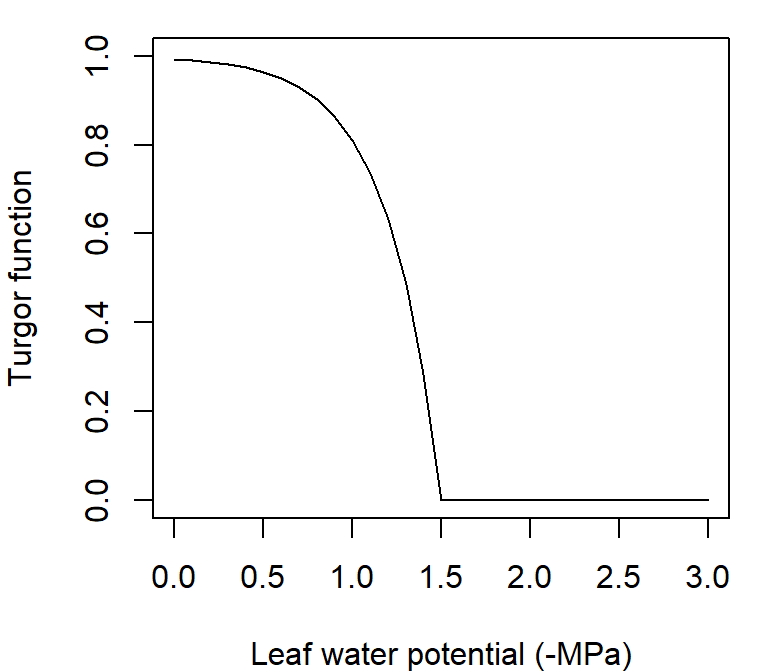
\includegraphics{medfatebook_files/figure-latex/unnamed-chunk-71-1} \end{center}

Obviously, if carbon pools are not considered \(f_{conc} = 1\).

Growth modulation due to temperature is incorporated through \(f_{temp}(T_{mean})\), using a truncated parabolic function as in Poyatos et al. (2007):
\begin{equation}
f_{temp}(T) = \frac{(T-T_{low}) \cdot (T_{high}-T)}{(T_{opt}-T_{low}) \cdot (T_{high}-T_{opt})}
\end{equation}
where \(0 \leq f_{temp}(T) \leq 1\), \(T_{low}\) and \(T_{high}\) minimum and maximum temperature values for growth and \(T_{opt}\) is the optimum growth temperature.

\begin{center}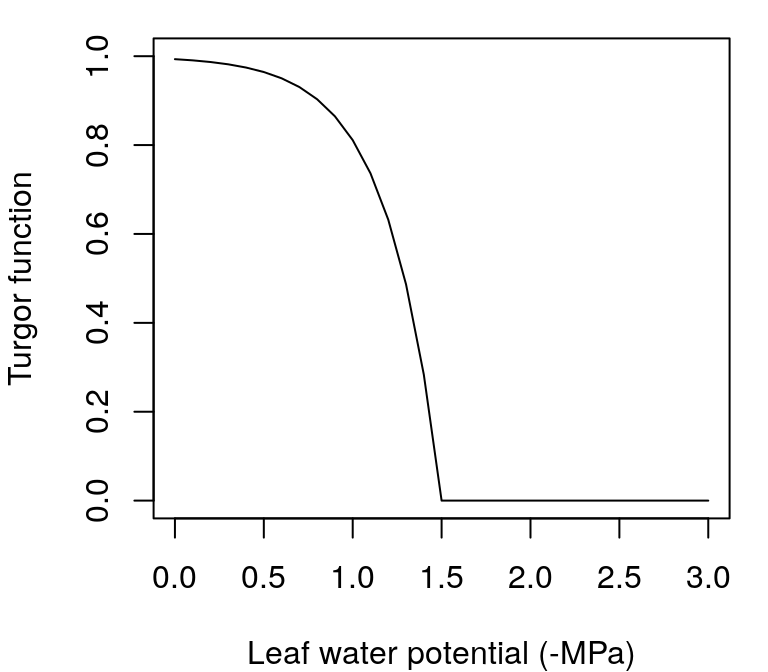
\includegraphics{medfatebook_files/figure-latex/unnamed-chunk-72-1} \end{center}

The rate of daily increase in sapwood area taking into account sink limitations is (\(\Delta SA_{sink}\); \(cm^2\)):
\begin{equation}
\Delta SA_{sink} = RGR_{\max} \cdot SA \cdot f_{turgor}(\Psi_{leaf}) \cdot f_{conc} \cdot f_{temp}(T_{mean})
\end{equation}
where \(RGR_{\max}\) is the user-defined, species-specific maximum relative growth rate in sapwood area (in \(cm^2·cm^{-2}\)), which can incorporate nutrient deficiency effects.

The final growth rate of sapwood area per individual, \(\Delta SA_{growth}\) (in \(cm^2\)), is found by combining the potential increase in sapwood area according to availability and cost with the sink limitations:
\begin{equation}
\Delta SA_{growth} = \min(\Delta SA_{available}, \, \Delta SA_{sink})
\end{equation}
If carbon pools are considered the actual carbon growth consumption (i.e. \(C_{cost,overall} \cdot \Delta SA_{growth}\)) has to be subtracted from \(C_{fast}\):
\begin{equation}
C_{fast} = C_{fast} - C_{cost,overall} \cdot \Delta SA_{growth}
\end{equation}

Sapwood area is updated considering both new sapwood formation and sapwood conversion to heartwood (\(\Delta SA_{turnover}\)):
\begin{equation}
SA = SA + \Delta SA_{growth} - \Delta SA_{turnover} 
\end{equation}
After updating sapwood area, the model updates living, expanded and dead leaf area accordingly:
\begin{eqnarray}
LAI^{live} &=& LAI^{live} + N \cdot (\Delta SA_{growth} - \Delta SA_{turnover}) \cdot Hv \\
LAI^{\phi} &=& LAI^{live}\,\cdot\phi \\
LAI^{dead} &=& LAI^{dead} + N \cdot \Delta SA_{turnover} \cdot Hv 
\end{eqnarray}

During non-drought periods the state variables regulating drought effects are kept at initial values (i.e. \(\Psi_{\min} = 0\) and \(LAI^{predrought} = LAI^{live}\)).

\hypertarget{leaf-area-losses-during-drought-periods}{%
\section{Leaf area losses during drought-periods}\label{leaf-area-losses-during-drought-periods}}

During drought-periods (i.e.~if \(f_{turgor}(\Psi_{leaf})=0\)) cavitation may occur. However, cavitation is applied at the leaf area level and not at the sapwood area level. During drought periods reductions of live leaf area can come from either sapwood conversion into heartwood or cavitation. First, the model compares the current \(\Psi_{leaf}\) value with \(\Psi_{\min}\) the minimum potential experienced since drought started:
\begin{equation}
\Psi_{\min} = \min(\Psi_{leaf}, \, \Psi_{\min})
\end{equation}
Then the model determines the proportion of embolized conducts as the complement of hydraulic conductance corresponding to \(\Psi_{\min}\), relative to the maximum hydraulic conductance. If the transpiration mode is ``Simple'', this is done using a whole-plant conductance function:
\begin{equation}
P_{embolism}=1- K(\Psi_{\min}) = \exp \left \{\ln{(0.5)}\cdot \left[ \frac{\Psi_{\min}}{\Psi_{extract}} \right] ^r \right \} 
\end{equation}
where \(\Psi_{extract}\) is the potential at which conductance is 50\% of maximum and \(r=3\). If the transpiration mode is ``Complex'', \(P_{embolism}\) is calculated using the stem-leaves vulnerability curve:
\begin{equation}
P_{emb}= 1- \frac{k_{stem}(\Psi_{\min})}{k_{stem}(0)} = 1 - \exp \left \{-\left[ \frac{\Psi_{\min}}{d_{stem}} \right] ^{c_{stem}} \right \} 
\end{equation}
Since leaf area reduction may also come from sapwood conversion into heartwood, the model determines which process leads to a larger reduction in leaf area:
\begin{equation}
LAI^{live} = \min(LAI^{live} - N \cdot \Delta SA_{turnover} \cdot Hv , \, LAI^{predrought} \cdot (1 - P_{emb}))
\end{equation}
and expanded leaf area (\(LAI^{\phi}\)) and dead leaf area (\(LAI^{dead}\)) are modified accordingly.

\hypertarget{transfer-between-carbon-pools}{%
\section{Transfer between carbon pools}\label{transfer-between-carbon-pools}}

If two carbon pools are considered then carbon can be transferred from one to the other. The model assumes that the direction of transfer depends on the C concentration in the fast pool. When the pool is at full capacity its C should be converted to long-term storage, whereas if the pool is empty C stored in the slow pool should be mobilised. The relative rate of transfer (\(r_{transfer}\); in \(g C·g C^{-1}\)) is modelled using a sigmoidal function:
\begin{equation}
r_{transf} = 0.1 \cdot \frac{2}{1+\exp \left(-5 \cdot \frac{(C_{fast}/C_{fast, \max})-0.5}{0.5}\right)}-1
\end{equation}

\begin{center}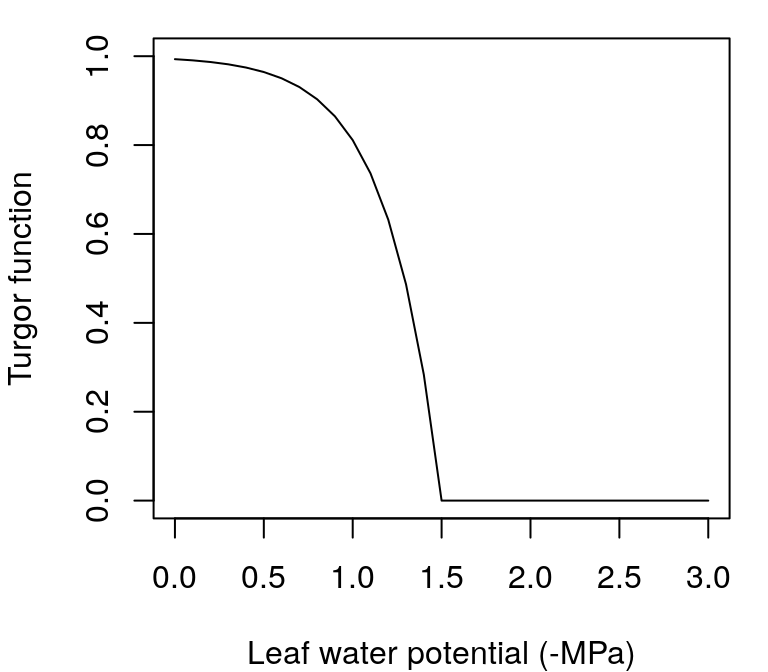
\includegraphics{medfatebook_files/figure-latex/unnamed-chunk-73-1} \end{center}

where \(0.1\) indicates that the maximum daily transfer rate is 10\% of the source C pool size. If \(r_{transf}<0\) then \(-r_{transf} \cdot C_{slow, \max}\) g of carbon are taken from the slow C pool and 90\% of this amount is added into the fast C pool (the remaining 10\% is assumed to be the transfer cost). Similarly, if \(r_{transf}>0\) then \(r_{transf} \cdot C_{fast, \max}\) g of carbon are taken from the fast C pool and 90\% of this amount is added into the slow C pool (again, the remaining 10\% is assumed to be the transfer cost). The amounts of C transferred are also limited by the amount that would be needed to fill the sink pool (i.e., if the sink pool is already full, no carbon is transferred).

\hypertarget{update-of-maximum-stem-conductance}{%
\section{Update of maximum stem conductance}\label{update-of-maximum-stem-conductance}}

The inclusion of \(Hv\) in the initialization of \(SA\) and in growth equations causes sapwood area and leaf area to maintain a constant ratio equal to \(Hv\). However, this rule may be broken by leaf phenology or when losing leaves because of drought stress. Leaf area reductions cause transpirational demand to be reduced accordingly. Moreover, in the case of Complex's transpiration mode leaf loss causes variations in leaf area to sapwood area ratio, which may become lower than \(Hv\) and, hence, maximum stem hydraulic conductance may increase. Tree size controls much of the variation in stem hydraulic conductance, since hydraulic path length increases with tree height. We modelled stem conductance per leaf area unit (\(k_{stem, \max}\); in \(mmol·m^{-2}·s^{-1}·MPa^{-1}\)) as a function of species-specific xylem conductivity (\(k_{xylem, \max}\); in \(kg·m^{-1}·s^{-1}·MPa^{-1}\)), leaf area to sapwood area ratio and tree height \citep{Christoffersen2016}:
\begin{equation}
k_{stem, \max} = \frac{1000}{0.018} \cdot \frac{k_{xylem, \max} \cdot (SA/10000)}{(H/100) \cdot LA^{\phi}} \cdot \chi_{taper}
\end{equation}
where \(\chi_{taper}\) is a factor to account for taper of xylem conduit with height \citep{Savage2010, Christoffersen2016}, 0.018 is the molar weight of water (in kg·mol\(^{-1}\)). This way, if the leaf-to-sapwood area ratio decreases with tree height, as has been documented in several species (McDowell et al.~2002), the decreasing conductance effects with height may be partially overcome \citep{Christoffersen2016}. A drought-induced decrease in \(LA^{\phi}\) alleviate drought effects (i.e.~a lower decrease in water potential across the stem for the same flow) because of an increase in conductance.

\hypertarget{update-of-structural-variables}{%
\chapter{Update of structural variables}\label{update-of-structural-variables}}

Unlike functional variables, structural variables are updated for simplicity once a year only (or before the end of the simulated period).

\hypertarget{tree-diameter-height-and-crown-ratio}{%
\section{Tree diameter, height and crown ratio}\label{tree-diameter-height-and-crown-ratio}}

In the case of tree cohorts, the cumulated new sapwood area (\(\sum{SA_{growth}}\)) is translated to an increment in DBH (\(\Delta DBH\), in cm) following:
\begin{equation}
\Delta DBH = 2 \cdot \sqrt{(DBH/2)^2+(\sum{SA_{growth}}/\pi)} - DBH
\end{equation}
Furthermore, the model assumes that increments in height are linearly related to increments in diameter through a function \(f_{HD}\) (Lindner et al.~1997):

\begin{equation}
\Delta H = f_{HD} \cdot \Delta DBH
\end{equation}

Hence, \(f_{HD}\) represents the height increment (in cm) per each cm of diameter increment. It was customary in forest gap models to prevent height from being larger than a species-specific value \(H_{\max}\), so that beyond some point trees only grew in size by increasing their diameter. Moreover, light conditions influence growth in height with trees living under the shade of others generally showing larger increases in height than trees living in open conditions. Hence, our formulation for \(f_{HD}\) is \citep{Lindner1997, Rasche2012}:
\begin{equation}
f_{HD} = \left[f_{HD,\min} \cdot L + f_{HD,\max} \cdot (1-L) \right] \cdot \left( 1 - \frac{H-137}{H_{\max} - 137} \right)
\end{equation}
where \(f_{HD,\min}\) would be the height-diameter ratio for a tree of 137 cm height growing in full light and \(f_{HD,\max}\) would be the same ratio for a tree of the same height growing in the shadow. This formulation seems slightly easier to calibrate than that presented in \citet{Rasche2012}. \(H_{\max}\) could be dependent on environmental conditions, but we skip this here, because environmental conditions already affect growth rate and carbon balance.

After updating tree diameter (\(DBH\)) and tree height (\(H\)), the model updates tree crown ratio (\(CR\)) by applying allometric relationships that take into account tree size and competition (see details in vignette XX).

\hypertarget{shrub-height-and-cover}{%
\section{Shrub height and cover}\label{shrub-height-and-cover}}

Since shrub structural variables are height and cover, shrub growth is done in a way somewhat different from trees. Shrubs are often multi-stemmed (some trees also are), so that increases in sapwood area are not easily related to diameter growth. Since leaf biomass is related to sapwood area, one may model shrub growth assuming an allometric relationship between phytovolume of individual shrub crowns and photosynthetic biomass. This strategy entails that shrubs may grow or shrink in size depending on their C balance, in the same way that tree crowns would become denser or sparser depending on their C balance. Hence, shrubs can be understood as crowns in the floor.

Starting from live leaf area (\(m^2·m^{-2}\)) we can calculate the foliar weight per shrub individual (in \(kg · ind^{-1}\)):
\begin{equation}
W_{leaves} = \frac{LAI^{live}} {(N/10000) \cdot SLA}
\end{equation}
An allometric relationship relating the biomass of leaves plus small branches and crown phytovolume (\(PV\); in \(m^3·ind^{-1}\)) can be drawn from fuel calculations:
\begin{equation}
W_{leaves+branches} = W_{leaves} \cdot r_{6.35}  = a_{bsh} \cdot PV^{b_{bsh}}
\end{equation}
where \(a_{bsh}\) and \(b_{bsh}\) are allometric relationships and \(r_{6.35}\) is a species-specific ratio relating the dry weight of leaves plus small branches to the dry weight of leaves. Inverting this relationship we obtain an expression of shrub crown phytovolume:
\begin{equation}
PV = \left[\frac{W_{leaves} \cdot r_{6.35}}{a_{bsh}}\right]^{1/b_{bsh}}
\end{equation}
Phytovolume is defined as the volume occupied by the shrub crown, i.e.:
\begin{equation}
PV =  (A_{sh}/10000) \cdot (H/100) \cdot CR
\end{equation}
where \(A_{sh}\) is the area of a single shrub individual (in \(cm^2\)). If we use the following quadratic relationship between \(A_{sh}\) and \(H\):
\begin{equation}
A_{sh} = a_{ash} \cdot H^2
\end{equation}
we can calculate shrub height from phytovolume using:
\begin{equation}
H = \left[\frac{10^6 \cdot PV}{a_{ash} \cdot CR}\right]^{1/3}
\end{equation}
Finally, the new value for shrub cover (in percent) can be obtained from \(H\) and \(N\) (in ind·ha\(^{-1}\)):
\begin{equation}
Cover = 100 \cdot (N/10000) \cdot (A_{sh}/10000) = \frac{N \cdot a_{ash} \cdot H^2}{10^6}
\end{equation}
Note that crown ratio for shrubs is assumed constant in the model. Like for trees, shrub height is limited to a maximum height \(H_{\max}\). However, unlike trees, shrubs are not allowed to continue growing once this maximum size is attained. When the estimated height is over the maximum value, the exceeding amount of live leaf area is allocated to dead live area.

\hypertarget{part-static-modules}{%
\part{Static modules}\label{part-static-modules}}

\hypertarget{fuel-characteristics-and-fire-behaviour}{%
\chapter{Fuel characteristics and fire behaviour}\label{fuel-characteristics-and-fire-behaviour}}

\hypertarget{purpose}{%
\section{Purpose}\label{purpose}}

Functions \texttt{fuel\_FCCS()} and \texttt{fire\_FCCS()} allow calculating potential fire behaviour for forest inventory plots. Formulation of fuel characteristics and fire behaviour is an adaptation of the Fuel Characteristics Classification System \citep[FCCS;][]{Prichard2013}. In FCCS, fuelbed is divided into six strata, including canopy, shrub, herbaceous vegetation, dead woody materials, leaf litter and ground fuels. All except ground fuels are considered here. The intensity of burning depends on several factors, including topography, wind conditions, fuel structure and its moisture content, which is determined from antecedent and current meteorological conditions. A modification of the Rothermel's \citeyearpar{Rothermel1972} model is used to calculate the intensity of surface fire reaction (in \(kW/m^2\)) and the rate of fire spread (in \(m/min\)) of surface fires assuming a steady-state fire. Both quantities are dependent on fuel characteristics, windspeed and direction, and topographic slope and aspect. The model returns the following results: (1) Fuel characteristics by stratum; (2) Surface fire behavior (i.e.~reaction intensity, rate of spread, fireline intensity and flame length); (3) Crown fire behavior; (4) Fire potential ratings of surface fire behavior and crown fire behavior.

\hypertarget{input-data}{%
\section{Input data}\label{input-data}}

\hypertarget{forest-inventory-plot-data}{%
\subsection{Forest inventory plot data}\label{forest-inventory-plot-data}}

The input data for tree cohorts are:

\begin{itemize}
\tightlist
\item
  \(SP_i\): Species identity\}
\item
  \(DBH_i\): Diameter at breast height (in cm) of the representative tree.
\item
  \(H_i\): Height (in cm) of the representative tree.
\item
  \(N_i\): Cohort density (in \(ind.\cdot ha^{-1}\)).
\end{itemize}

The input data for shrub cohorts are:

\begin{itemize}
\tightlist
\item
  \(SP_i\): Species identity
\item
  \(C_i\): Plant cover (in percent).
\item
  \(H_i\): Mean plant height (in cm).
\end{itemize}

Cohorts are not distinguished for the herbaceous stratum, and the variables needed are:

\begin{itemize}
\tightlist
\item
  \(C_{he}\): Herbaceous cover (in percent).
\item
  \(H_{he}\): Mean herb height (in cm).
\end{itemize}

Finally, the model also requires the percent cover of trees in the canopy (\(C_{ca}\)). This is easily available from forest inventory data, but could also be derived from the description of tree cohorts.

\hypertarget{species-specific-parameters}{%
\subsection{Species-specific parameters}\label{species-specific-parameters}}

\begin{itemize}
\tightlist
\item
  \(cr(SP_i)\): {[}\texttt{cr}{]}: Ratio between crown length and total height for shrubs.
\item
  \(a_{fbt}, b_{fbt}, c_{fbt}, d_{fbt}\) {[}\texttt{a\_fbt}, \texttt{b\_fbt}, \texttt{c\_fbt}, \texttt{d\_fbt}{]}: Regression coefficients used to calculate foliar biomass of an individual tree from its \(DBH\) and the cummulative basal area of larger trees.
\item
  \(a_{ash}\) {[}\texttt{a\_ash}{]}: Regression coefficient relating the square of shrub height with shrub area.
\item
  \(a_{bsh}\) and \(b_{bsh}\) {[}\texttt{a\_bsh}, \texttt{b\_bsh}{]}: Allometric coefficients relating phytovolume with dry weight of shrub individuals.
\item
  \(r_{6.35}(SP_i)\) {[}\texttt{r635}{]}: Ratio between the weight of leaves plus branches and the weight of leaves alone for branches of 6.35 mm.
\item
  \(\rho_p(SP_i)\) {[}\texttt{PD}{]}: Particle density.
\item
  \(\sigma(SP_i)\) {[}\texttt{SAV}{]}: Surface-area-to-volume ratio of the small fuel (1h) fraction (leaves and branches \textless{} 6.35mm).
\item
  \(h(SP_i)\) {[}\texttt{HeatContent}{]}: High fuel heat content.
\item
  \(\eta_{F}(SP_i)\) {[}\texttt{Flammability}{]}: Flammability value (either 1 or 2 for normal or high, respectively).
\item
  \(LD(SP_i)\) {[}\texttt{LeafDuration}{]}: Leaf duration (in years).
\item
  \(LI(SP_i)\) {[}\texttt{PercentLignin}{]}: Percentage of lignin in leaves.
\end{itemize}

\hypertarget{other-inputs}{%
\subsection{Other inputs}\label{other-inputs}}

Other inputs may be given by expert opinion or they may be calculated from another model. Specifically, for each plant cohort (and for any day of application) the fire behaviour model requires:
+ \(P_{dead,i}\): Proportion of the plant that is dead.
+ \(M_i\): Foliar moisture value (in percent of dry weight).

Analogously, the same variables are needed for the herbaceous stratum.
+ \(P_{dead,he}\): Proportion of herb fuels that respond to humidity changes as 1-h dead fuels.
+ \(M_{live,he}\): Foliar moisture value of live herb fuels (in percent of dry weight).

The model also needs the following input parameters:

\begin{itemize}
\tightlist
\item
  \(M_{dead}\): the moisture of 1-h dead fuels (in percent of dry weight).
\item
  \(U\): Midflame windspeed (in \(m\cdot s^{-1}\)).
\item
  \(S\): Slope (in percent).
\end{itemize}

\hypertarget{fuel-characteristics}{%
\section{Fuel characteristics}\label{fuel-characteristics}}

\hypertarget{cohort-fuel-loading}{%
\subsection{Cohort fuel loading}\label{cohort-fuel-loading}}

Here we consider as burnable fuels foliage and branches up to 6.35 mm = 0.25 in in diameter. The same consideration applies to both trees and shrubs.

\hypertarget{tree-cohorts}{%
\subsubsection{Tree cohorts}\label{tree-cohorts}}

Foliar biomass for a single tree of cohort \(i\) (\(FB_{tree,i}\); in \(kg\)) is calculated using:
\begin{equation}
FB_{tree,i} = a_{fbt} \cdot DBH_{i}^{b_{fbt}}\cdot e^{c_{fbt}\cdot BAL_i} \cdot DBH_{i}^{d_{fbt} \cdot BA_{sup}}
\end{equation}
where \(DBH_{i}\) is the diameter of the tree (in \(cm\)), \(BAL_i\) is the cummulative basal area (\(m^2\cdot ha^{-1}\)) of trees having a larger diameter, and \(a_{fbt}\), \(b_{fbt}\), \(c_{fbt}\) and \(c_{fbt}\) are species-specific regression coefficients. The foliar biomass of the whole tree cohort (\(FB_{i}\); in \(kg\cdot m^{-2}\)) is obtained multiplying tree foliar biomass by tree density (\(N_{i}\); in \(ind.\cdot ha^{-1}\)):
\begin{equation}
FB_{i} = FB_{tree,i}\cdot (N_{i}/10000)
\end{equation}
Fine fuel loading for the tree cohort (\(W_{i}\); in \(kg\cdot m^{-2}\)), including its leaves and branches with diameter up to 6.35 mm = 0.25 in, is then calculated using:
\begin{equation}
W_{i} = r_{6.35}(SP_i)\cdot FB_{i}
\end{equation}
where \(r_{6.35}(SP_i)\) is the ratio between the weight of leaves plus branches and the weight of leaves alone for branches of 6.35 mm in diameter for the species of cohort \(i\). The biomass corresponding to branches of less than \textless{} 6.35 mm (\(SBB_{i}\), also in \(kg\cdot m^{-2}\)) is obtained by subtraction:
\begin{equation}
SBB_{i} = (r_{6.35}(SP_i)-1)\cdot FB_{i}
\end{equation}
Whereas \(W_{i}\) is the cohort loading variable influencing fire behavior, \(FB_{i}\) and \(SBB_{i}\) are cohort variables used to estimate fine dead woody and leaf litter loadings.

\hypertarget{shrub-cohorts}{%
\subsubsection{Shrub cohorts}\label{shrub-cohorts}}

To calculate the fuel loading of a shrub cohort (including both leaves and stems up to 6.35mm), we first determine \(A_{sh,i}\), the area (in \(cm^2\)) occupied by one average individual of height \(H_{i}\) (in \(cm\)), using the quadratic relationship:
\begin{equation}
A_{sh,i} = a_{ash} \cdot H_{i}^2
\end{equation}
where \(a_{ash}\) is a species-specific parameter. The model then estimates the dry weight of leaves and branches up to 6.35mm in diameter (\(B_{sh,i}\), in kg) of this average individual, using an allometric relationship with shrub crown phytovolume assuming a cylinder (in \(cm^3\)):
\begin{equation}
B_{sh,i} = a_{bsh} \cdot (A_{sh,i}\cdot H_{i}\cdot cr(SP_i))^{b_{bsh}}
\end{equation}
where \(a_{bsh}\) and \(b_{bsh}\) are species-specific parameters and \(cr(SP_i)\) is a species-specific crown ratio (a proportion between 0 and 1, the ratio between crown length and total height). Shrub density (\(N_{i}\); in \(ind.\cdot m^{-2}\)) can be grossly estimated from percent cover (\(C_{i}\), in percent) and \(A_{sh,i}\) (in \(cm^{-2}\)):
\begin{equation}
N_{i} = \frac{C_{i}/100}{A_{sh,i}/10000}
\end{equation}
The fine fuel loading of a shrub cohort \(W_{i}\), in \(kg \cdot m^{-2}\)) is simply the product of \(B_{sh,i}\) (\(kg\) of dry weight) and \(N_{i}\):
\begin{equation}
W_{i} =  B_{sh,i}\cdot N_{i}
\end{equation}
Our procedure differs from \citet{Prichard2013} because they calculate first total biomass of the shrub species and then consider the percentage of total weight that corresponds to leaves and small branches. Foliar biomass and small branch biomass (both in \(kg \cdot m^{-2}\)) can be obtained using the species-specific ratio \(r_{6.35}(SP_i)\):
\begin{eqnarray}
FB_{i} &=&  W_{i}/r_{6.35}(SP_i)\\
SBB_{i} &=& W_{i} - FB_{i}
\end{eqnarray}
If not known, \(r_{6.35}(SP_i)\) can be set to a default value of 2 (equivalent to \%50 of weight corresponding to leaves).

\hypertarget{vertical-structure-of-fuels}{%
\subsection{Vertical structure of fuels}\label{vertical-structure-of-fuels}}

\hypertarget{strata-definition}{%
\subsubsection{Strata definition}\label{strata-definition}}

The Fuel Characteristics Classification System (FCCS) on which this document is based, defines six fuel strata \citep{Prichard2013}:

\begin{itemize}
\tightlist
\item
  \emph{Canopy}: Trees, snags and ladder fuels.
\item
  \emph{Shrubs}: Primary and secondary layers.
\item
  \emph{Non-woody vegetation (herbs)}: grasses, sedges, rushes and forbs.
\item
  \emph{Woody fuels}: All downed and dead wood, sound wood, rotten wood and stumps.
\item
  \emph{Litter-lichen-moss}: Lichen, litter and moss layers.
\item
  \emph{Ground fuels}: Duff, basal accumulation and squirrel middens.
\end{itemize}

Shrubs, herbs and woody fuels are constitute the \textbf{upper surface fuels}, whereas herbs and woody fuels alone consitute the \textbf{lower surface fuels}. FCCS summarizes and calculates characteristics for each fuelbed stratum and layer. Our model estimates fuel loading and characteristics for canopy, shrub, non-woody vegetation, as well as fine (1h) woody fuels and litter fuels. Larger woody fuels (10h or 100h) could be considered if information about forest management actions is available. Ground fuels are not included here.

\hypertarget{vertical-distribution-of-tree-and-shrub-fuels}{%
\subsubsection{Vertical distribution of tree and shrub fuels}\label{vertical-distribution-of-tree-and-shrub-fuels}}

For all tree or shrub cohorts fuels are assumed to be homogeneously distributed between the crown base height and the total height (\(H_i\)). Crown base height (\(H_{b,i}\); in cm) is defined as the height corresponding to the first living branch expressed as a fraction of total height. It is calculated from the crown ratio (\(CR\); a proportion between 0 and 1), i.e.~the ratio between crown length and total height:
\begin{equation}
H_{b,i} = H_{i} \cdot (1 - CR_i)
\label{eq:CrownHeight}
\end{equation}
In the case of shrubs the crown ratio is simply equal by a species-specific parameter: \(CR_i = cr(SP_i)\). In the case of trees, the crown ratio is modelled as a function of tree size and stand competition, following a modification of the logistic equation of \citet{Hasenauer1996}:
\begin{equation}
CR_i = \frac{1}{1+e^{-(a_{cr}+b_{1cr}\cdot HD +b_{2cr} \cdot (H_i/100)+b_{3cr} \cdot DBH_i^2+c_{1cr} \cdot BAL_i + c_{2cr} \cdot ln(CCF))}}
\end{equation}
where \(HD = H_i/(100\cdot DBH_i)\) is the height to diameter ratio (in \(m\cdot cm^{-1}\)), \(H_i\) is the tree height, \(DBH_i\) is the diameter, \(CCF\) is the crown competition factor and \(a_{cr}\), \(b_{1cr}\), \(b_{2cr}\), \(b_{3cr}\), \(c_{1cr}\) and \(c_{2cr}\) are species-specific parameters. The crown competition factor is in turn calculated using \citep{Krajicek1961}:
\begin{equation}
CCF = \sum_{i}{N_i \cdot MCA_i}= \sum_{i}{N_i \cdot \pi \cdot (CW_i/2)^2/100}
\end{equation}
where \(N_i\) is the tree density, \(MCA_i\) is the maximum crown area (in percent of unit area) and \(CW_i\) is the crown width (in m) assuming an open-grown tree, estimated from an allometric relationship with tree diameter:
\begin{equation}
CW_i = a_{cw}\cdot BDH_i^{b_{cw}} 
\end{equation}
where again \(a_{cw}\) and \(b_{cw}\) are species-specific parameters.

The loading of a cohort that occurs within a given height interval of limits \(H_1\) and \(H_2\) is calculated as:
\begin{equation}
W_i(H_1, H_2) = W_i\cdot p_i(H_1, H_2)
\end{equation}
where \(p_i(H_1, H_2)\) is the proportion of the crown of cohort \(i\) that corresponds to the height interval \((H_1, H_2)\):
\begin{equation}
p_i(H_1, H_2) = \frac{\max(0, \min(H_i, H_2) - \max(H_{b,i}, H_1))}{H_{i}-H_{b,i}}
\end{equation}

\hypertarget{fuel-bulk-density-profile}{%
\subsection{Fuel bulk density profile}\label{fuel-bulk-density-profile}}

Knowing at which height fuels are placed, the \textbf{fuel bulk density profile} \citep{Reinhardt2006} is defined for any given interval \((H_1, H_2)\) as the bulk density (\(kg/m^3\)) of fine fuels corresponding to that interval:
\begin{equation}
BDP(H_1, H_2) = \frac{\sum_{i} W_i(H_1, H_2)}{H_2-H_1}
\end{equation}
Canopy bulk density normally ranges between 0 and 0.4 \(kg/m^3\) \citep{Scott2002}. \citet{Sando1972} arbitrarily defined canopy base height as the lower vertical 0.3-m section with a weight greater than \(0.01124 kg/m^3\). A user-defined threshold \(t_{BDP}\) (in \(kg/m^3\)) in 0.1-m sections is used to differentiate the surface fuelbed from canopy fuels. Using this threshold the model calculates the following three heights \citep{Reinhardt2006}:

\begin{itemize}
\tightlist
\item
  \emph{Shrub stratum base height}, \(H_{sb}\) (in \(cm\)): the minimum height between 0 and 2 m where fuel bulk density is larger than \(t_{BDP}\).
\item
  \emph{Shrub stratum top height}, \(H_{st}\) (in \(cm\)): the maximum height between 0 and 2 m where fuel bulk density larger than \(t_{BDP}\). With this definition \(h_{s}\) cannot be higher than 2 m (corresponding to fuel model 4 in Anderson 1982).
\item
  \emph{Canopy base height}, \(H_{cb}\) (in \(cm\)): In terms of its consequences to crown fire initiation, canopy base height can be defined as the lowest height above the ground at which there is sufficient canopy fuel to propagate fire vertically through the canopy. It is calculated as the minimum height over \(H_st\) when the bulk density starts again to be larger than \(t_{BDP}\).
\item
  \emph{Canopy top height}, \(H_{ct}\) (in \(cm\)): the maximum height where bulk density is larger than \(t_{BDP}\).
\item
  \emph{Canopy gap}, \(H_{gap}\) (in \(cm\)): the difference between \(H_{cb}\) and \(H_{st}\). The canopy gap is used to calculate crown initiation potential.
\end{itemize}

The following figure illustrates the definition and analysis of the fuel bulk density profile for a given forest stand. Following \citet{Mitsopoulos2007}, a threshold \(t_{BDP} = 0.04\) has been used to determine shrub and canopy heights.

\begin{center}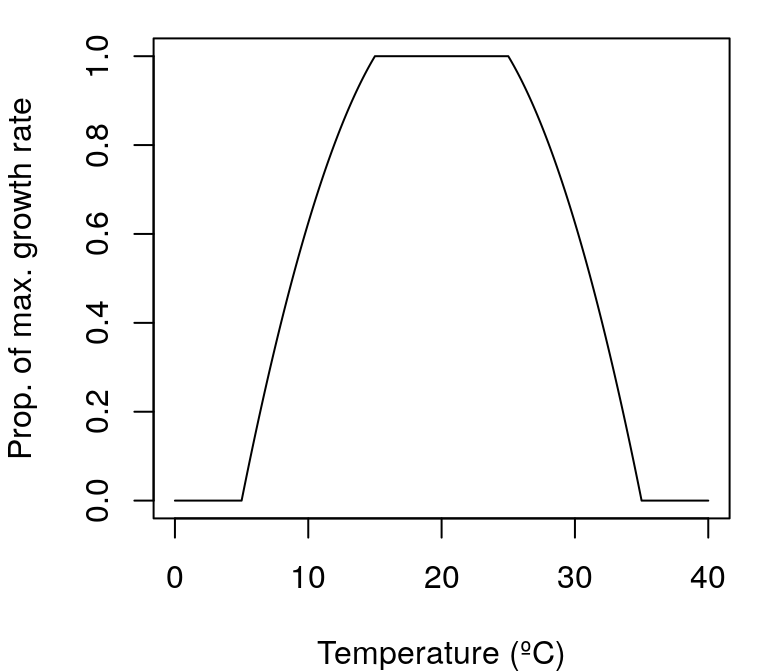
\includegraphics{medfatebook_files/figure-latex/unnamed-chunk-75-1} \end{center}

\hypertarget{fuel-loading-w-and-fuel-depth-delta}{%
\subsection{\texorpdfstring{Fuel loading (\(w\)) and fuel depth (\(\delta\))}{Fuel loading (w) and fuel depth (\textbackslash{}delta)}}\label{fuel-loading-w-and-fuel-depth-delta}}

\hypertarget{canopy-stratum}{%
\subsubsection{Canopy stratum}\label{canopy-stratum}}

Canopy loading (in \(kg\cdot m^{-2}\)) is the sum of (tree and shrub) cohort loadings above 2 m (i.e.~200 cm):
\begin{equation}
w_{ca} = \sum_{i}w_{i,ca} =\sum_{i}{W_i(200, \infty})
\end{equation}
where \(w_{i,ca}\) is the canopy stratum loading of cohort \(i\). Canopy depth (in \(m\)) is defined as the average of tree (or shrub) crown lengths above 2 m, weighted by the loadings of cohorts in the canopy:
\begin{equation}
\delta_{ca} = \frac{1}{100}\cdot\frac{\sum_{i}{w_{i,ca}\cdot (H_i - H_{b,i})\cdot p_{i,ca} }}{\sum_{i}{w_{i,ca}}}
\end{equation}
where the proportion of a tree (or shrub) cohort in the canopy stratum is \(p_{i,ca}=p_{i}(200,\infty)\).

\hypertarget{shrub-stratum}{%
\subsubsection{Shrub stratum}\label{shrub-stratum}}

Shrub loading (in \(kg\cdot m^{-2}\)) is the sum of (tree and shrub) cohort loadings between the ground and 2 m (i.e.~200 cm):
\begin{equation}
w_{sh} = \sum_{i}w_{i,sh} =\sum_{i}W_i(0, 200)
\end{equation}
where \(w_{i,sh}\) is the shrub stratum loading of cohort \(i\). The depth of the shrub stratum (in \(m\)) is defined as the average of tree (or shrub) crown lengths below 2 m, weighted by the loadings of cohorts in the shrub stratum:
\begin{equation}
\delta_{sh} = \frac{1}{100}\cdot \frac{\sum_{i}{w_{i,sh}\cdot (H_i - H_{b,i})\cdot p_{i,sh} }}{\sum_{i}{w_{i,sh}}}
\end{equation}
where the proportion of a shrub (or tree) cohort in the shrub stratum is \(p_{i,sh}=p_{i}(0,200)\).

\hypertarget{non-woody-stratum}{%
\subsubsection{Non-woody stratum}\label{non-woody-stratum}}

Herb percent cover and average herb height are transformed into herbaceous loading (\(kg\cdot m^{-2}\)) using (ref piropinos):
\begin{equation}
w_{he} = 0.014 \cdot C_{he} \cdot (H_{he}/100)
\end{equation}
The depth of the herbaceous stratum (in \(m\)) is simply the mean height of herbs:
\begin{equation}
\delta_{he} = H_{he}/100
\end{equation}

\hypertarget{woody-and-litter-strata}{%
\subsubsection{Woody and litter strata}\label{woody-and-litter-strata}}

In FCCS \citep{Prichard2013}, woody surface loading includes several fuel sizes. However, when calculating surface fire behavior \(w_{wo}\) includes 100\% of 1h fuels, 25\% of 10h fuels and 12.5\% of 100h fuels, which represents the material available for flaming combustion. Obtaining loading estimates for 10h- and 100h-fuels is very difficult without field fuel sampling. However, we might estimate 1h woody fuels and leaf litter from standing biomass of small branches (\textless{} 6.35mm) and leaves for trees and shrubs. Hence, our treatment of surface woody fuels includes only fine (1h) fuels.

Assuming a continuous input of litter, the variation in accumulated litter is described by a simple differential equation \citep{Birk1980}:
\begin{equation}
\frac{\mathrm{d}X}{\mathrm{d}t} = L - k\cdot X
\end{equation}
where \(k\) is the decay constant, \(L\) is the rate of litterfall and \(X\) is the litter mass accumulated in the forest floor. Assuming that litter mass has reached a steady state, \(X\) can be estimated as the ratio between \(L\) and \(k\). If litterfall is estimated as the total foliar biomass divided by leaf duration, the amount of steady state leaf litter corresponding to each tree and srhub cohort can be estimated using:
\begin{equation}
w_{li, i} = \frac{FB_i}{LD(SP_i) \cdot k_i}
\end{equation}
where \(FB_i\) is the foliar biomass of cohort \(i\), \(LD(SP_i)\) is the species-specific average leaf duration (in years) and \(k_i\) is the rate of decay of leaves of cohort \(i\), which is given by the regreession model of Meentemeyer (1978):
\begin{equation}
k_i = (-0.5365+0.00241\cdot AET) - (-0.01586+0.000056\cdot AET) \cdot LI(SP_i) 
\end{equation}
where \(LI(SP_i)\) is the species-specific percentage of lignin content in leaves and AET is actual evapotranspiration (default \(AET = 1000 mm\)). Litter loadings are summed for four litter types (short pine needles, long pine needles, other conifers, broadleaves). In the case of fine dead woody materials (small fallen branches), loading of small branches is taken as woody litter and it is assumed that small branch litterfall occurs at the same time as leaf litterfall (i.e.~according to leaf duration):
\begin{equation}
w_{wo} = \sum_{i}{w_{wo, i}} = \sum_{i}{\frac{SBB_i}{LD(SP_i)\cdot k_{wo}} }
\end{equation}
where \(k_{wo} = 0.95 y^{-1}\) is a constant rate of decomposition for small branches.

In FCCS, the depth of woody and LLM strata are inputs. In our case the depth of the woody and litter strata are estimated from the corresponding fuel loadings:
\begin{eqnarray}
\delta_{wo} &= w_{wo}/\rho_{b, wo}\\
\delta_{li} &= w_{li}/\rho_{b, li}
\end{eqnarray}
where \(\rho_{b, wo}\), \(\rho_{b, li}\) are the woody and litter bulk density (in \(kg\cdot m^{-3}\)), respectively. Litter bulk density \(\rho_{b,li}\) is calculated as a weighted average of litter types:
\begin{equation}
 \rho_{b,li} = \frac{\sum_{k}{ \rho_{b,k}\cdot w_{li,k}}}{\sum_{k} {\cdot w_{li,k}}}
\end{equation}
where \(k\) indicates litter type. The bulk density for litter types are {[}\citet{Prichard2013}; Table 1{]}:
\begin{eqnarray}
\rho_{b,shortneedlepine} &= \rho_{b,longneedlepine} = \rho_{b,otherconifer}= 1.65 lb\cdot ft^{-3} = 26.43 kg\cdot m^{-3}\\
\rho_{b,hardwood} &= 0.83 lb\cdot ft^{-3} = 13.30  kg\cdot m^{-3}
\end{eqnarray}

\hypertarget{other-fuel-characteristics}{%
\subsection{Other fuel characteristics}\label{other-fuel-characteristics}}

All the following characteristics are calculated in metric units (although British units are indicated to qualify specific values for compatibility).

\hypertarget{particle-density-rho_p}{%
\subsubsection{\texorpdfstring{Particle density (\(\rho_{p}\))}{Particle density (\textbackslash{}rho\_\{p\})}}\label{particle-density-rho_p}}

Particle density is the ratio of dry weight over volume for fuel particles (in \(kg\cdot m^{-3}\)). When species have different values, particle density averages for shrub and canopy strata can be obtained as:
\begin{eqnarray}
\rho_{p, sh} &= \frac{\sum_{i}{w_{i,sh} \cdot \rho_p(SP_i)}}{\sum_{i}{w_{i,sh}}}\\
\rho_{p, ca} &= \frac{\sum_{i}{w_{i,ca} \cdot \rho_p(SP_i)}}{\sum_{i}{w_{i,ca}}}
\end{eqnarray}
where \(\rho_p(SP_i)\) is the species-specific particle density. \(\rho_{p, he}\), \(\rho_{p, wo}\) and \(\rho_{p, li}\) are all set to a default value \(\rho_{p} = 400 kg\cdot m^{-3}= 25 lb\cdot ft^{-3}\) \citep{Prichard2013}.

\hypertarget{particle-volume-pv}{%
\subsubsection{\texorpdfstring{Particle volume (\(PV\))}{Particle volume (PV)}}\label{particle-volume-pv}}

Particle volume is defined as the volume of particles per surface area (in \(m^3\cdot m^{-2}\)). Is calculated as dry weight loading divided by particle density. If species have different particle density values, the particle volume for canopy (\(PV_{ca}\)) and shrub(\(PV_{sh}\)) strata can be calculated using:
\begin{eqnarray}
PV_{ca} &= \sum_{i}{PV_{i,ca}} = \sum_{i}{w_{i,ca}/\rho_{p}(SP_i)}\\
PV_{sh} &= \sum_{i}{PV_{i,sh}} = \sum_{i}{w_{i,sh}/\rho_{p}(SP_i)}
\end{eqnarray}
where \(PV_{i,ca}\) and \(PV_{i,sh}\) are the particle volume of cohort \(i\) in the canopy and shrub strata, respectively. The particle volume for woody and herb strata are simply:
\begin{eqnarray}
PV_{wo} &= w_{wo}/\rho_{p,wo}\\
PV_{he} &= w_{he}/\rho_{p,he}
\end{eqnarray}
The particle volume for the litter stratum is the sum of particle volume of litter components:
\begin{equation}
PV_{li} = \sum_{i}{PV_{li,k}} = \sum_{i}{w_{li,k}/\rho_{p, li}}
\end{equation}

\hypertarget{packing-ratio-beta}{%
\subsubsection{\texorpdfstring{Packing ratio (\(\beta\))}{Packing ratio (\textbackslash{}beta)}}\label{packing-ratio-beta}}

The proportion of fuelbed stratum volume occupied by fuel particles is an important factor to predict fire behavior. At low packing ratios (low particle density) fire intensity is limited by excessive heat loss. At high packing ratios (high particle density), lack of oxygen limits combustion. The packing ratios for the canopy and shrub stratum (\(\beta_{ca}\) and \(\beta_{sh}\); dimensionless) are given by:
\begin{eqnarray}\\eqref{eq:packingratioshrub}
\beta _{ca} &= \frac{PV_{ca}}{\delta_{ca}}\\
\beta _{sh} &= \frac{PV_{sh}}{\delta_{sh}}
\end{eqnarray}
where \(w_{i,ca}\) and \(w_{i,sh}\) are the contribution of cohort \(i\) to canopy and shrub strata loading (in \(kg\cdot m^{-2}\)), respectively, and \(\rho_p(SP_i)\) is the particle density (in \(kg\cdot m^{-3}\)) of fuels in cohort \(i\). The packing ratio for the herbaceous, woody and litter strata are:
\begin{eqnarray}
\beta _{he} &= \frac{PV_{he}}{\delta_{he}}\\
\beta _{wo} &= \frac{PV_{wo}}{\delta_{wo}}= \frac{\rho_{b,wo}}{\rho_{p,wo}}\\
\beta _{li} &= \frac{PV_{li}}{\delta_{li}}= \frac{\rho_{b,li}}{\rho_{p,li}}
\end{eqnarray}
Note that the packing ratio expressions for woody and litter strata as a ratio of bulk and particle density arises as a consequence of how fuel depth and particle volume are estimated.

\hypertarget{surface-area-to-volume-ratio-sigma}{%
\subsubsection{\texorpdfstring{Surface-area-to-volume ratio (\(\sigma\))}{Surface-area-to-volume ratio (\textbackslash{}sigma)}}\label{surface-area-to-volume-ratio-sigma}}

The surface-area-to-volume ratio (in \(m^2\cdot m^{-3}\)) for the canopy or shrub strata are calculated using weighted averages:
\begin{eqnarray}
\sigma_{ca} &= \frac{\sum_{i}{w_{i,ca} \cdot \sigma(SP_i)}}{\sum_{i}{w_{i,ca}}}\\
\sigma_{sh} &= \frac{\sum_{i}{w_{i,sh} \cdot \sigma(SP_i)}}{\sum_{i}{w_{i,sh}}}
\end{eqnarray}
where \(w_{i,ca}\) and \(w_{i,sh}\) are the contribution of cohort \(i\) to canopy and shrub strata loading (in \(kg\cdot m^{-2}\)), respectively, and \(\sigma(SP_i)\) is the species-specific surface-area-to-volume ratio. The surface-area-to-volume ratio of herbs is assumed constant \(\sigma_{he} = 11483 m^2\cdot m^{-3} = 3500 ft^2\cdot ft^{-3}\) and that of small (1-h) woody fuels is \(\sigma_{wo} = 1601.05 m^2\cdot m^{-3} = 488 ft^2\cdot ft^{-3}\). The surface-area-to-volume ratio for the litter stratum is:
\begin{equation}
\sigma_{li} = \frac{\sum_{k}{w_{li,k} \cdot \sigma_{k}}}{\sum_{k}{w_{li,k}}}
\end{equation}
and the surface-area-to-volume ratio for litter types are:
\begin{eqnarray}
\sigma_{shortneedlepine} &= 6562 m^{2}\cdot m^{-3}= 2000 ft^{2}\cdot ft^{-3}\\
\sigma_{longneedlepine} &= 4921 m^{2}\cdot m^{-3}= 1500 ft^{2}\cdot ft^{-3}\\
\sigma_{otherconifer} &= 8202 m^{2}\cdot m^{-3}= 2500 ft^{2}\cdot ft^{-3}\\
\sigma_{hardwood} &= 8202 m^{2}\cdot m^{-3}= 2500 ft^{2}\cdot ft^{-3}
\end{eqnarray}

\hypertarget{fuel-area-index-fai}{%
\subsubsection{Fuel area index (FAI)}\label{fuel-area-index-fai}}

The fuel area index (FAI) is the total fuel surface area per unit of ground area (unitless). It is analogous to leave area index (LAI), and it is used to calculate FCCS fire potentials \citep{Schaaf2007}. For shrub and canopy strata, FAI is calculated as:
\begin{eqnarray}
FAI_{ca} &= \sum_{i}{FAI_{i, ca}} = \sum_{i}{PV_{i,ca} \cdot\sigma(SP_i)}\\
FAI_{sh} &= \sum_{i}{FAI_{i, sh}}= \sum_{i}{PV_{i,sh} \cdot \sigma(SP_i)}
\end{eqnarray}
where \(FAI_{i, ca}\) and \(FAI_{i, sh}\) are the FAI of cohort \(i\) in the canopy and shrub strata, respectively. The FAI of herbs and woody strata are given by:
\begin{eqnarray}
FAI_{he} &= PV_{he} \cdot \sigma_{he}\\
FAI_{wo} &= PV_{wo} \cdot \sigma_{wo}
\end{eqnarray}
For the litter layer, FAI is calculated as a sum of FAI for litter components:
\begin{equation}
FAI_{li} = \sum_{k}{FAI_{li,k}} = \sum_{k}{PV_{li,k} \cdot \sigma_{k}}
\end{equation}

\hypertarget{moisture-m}{%
\subsubsection{\texorpdfstring{Moisture (\(M\))}{Moisture (M)}}\label{moisture-m}}

Live foliar moisture (in percent of dry weight) is also averaged across cohorts composing the shrub or canopy strata:
\begin{eqnarray}
M_{live, sh} &= \frac{\sum_{i}{w_{i,sh} \cdot M_i}}{\sum_{i}{w_{i,sh}}} \\
M_{live, ca} &= \frac{\sum_{i}{w_{i,ca} \cdot M_i}}{\sum_{i}{w_{i,ca}}}
\end{eqnarray}
Live foliar moisture of herb stratum (\(M_{live, he}\)) is an input. The moisture of dead plant in the canopy and shrub layers (\(M_{dead, ca}\) and \(M_{dead, sh}\)), the moisture of dead herbs (\(M_{dead, he}\)), as well as that of litter (\(M_{li}\)) and woody (\(M_{wo}\)) strata are all assumed equal to the moisture of 1-h dead fuels, which is an input of the model.

\hypertarget{proportion-of-dead-fuel-p_dead}{%
\subsubsection{\texorpdfstring{Proportion of dead fuel (\(P_{dead}\))}{Proportion of dead fuel (P\_\{dead\})}}\label{proportion-of-dead-fuel-p_dead}}

Woody and litter strata are dead fuels, but for canopy, shrub and herb strata the proportion of fuels that are dead are variable. The proportion of dead fuels in the herbaceous stratum (\(P_{dead,he}\)) is an input of the model, but for the shrub and canopy strata these are calculated from the proportion of dead fuels in each cohort:
\begin{eqnarray}
P_{dead,sh} &= \frac{\sum_{i}{w_{i,sh} \cdot P_{dead,i}}}{\sum_{i}{w_{i,sh}}} \\
P_{dead, ca} &= \frac{\sum_{i}{w_{i,ca} \cdot P_{dead,i}}}{\sum_{i}{w_{i,ca}}}
\end{eqnarray}

\hypertarget{low-heat-content-h}{%
\subsubsection{\texorpdfstring{Low heat content (\(h\))}{Low heat content (h)}}\label{low-heat-content-h}}

The low fuel heat content of each surface fuel stratum (in \(kJ\cdot kg^{-1}\)) is used for the calculation of reaction intensity. Heat content values are adjusted for live foliar moisture content in canopy, shrub and herb strata; and are left to the default value for woody and litter strata:
\begin{eqnarray}
h_{ca} &=& h_{ca, def} - (M_{live, ca}/100)\cdot V \\
h_{sh} &=& h_{sh, def} - (M_{live, sh}/100)\cdot V \\
h_{he} &=& h_{def} - (M_{live, he}/100)\cdot V \\
h_{wo} &=& h_{li} = h_{def}
\end{eqnarray}
where \(h_{def} = 18608 kJ\cdot kg^{-1} = 8000 Btu\cdot lb^{-1}\) is the default low heat content value for herbs, woody and litter strata, and \(V = 2596 kJ\cdot kg^{-1} = 1116 Btu\cdot lb\) is the latent heat of vaporisation of water. The default low heat of contents for the canopy and shrub strata (\(h_{ca, def}\) and \(h_{sh, def}\)) are calculated as a weighted average across cohorts:
\begin{eqnarray}
h_{ca, def} &=& \frac{\sum_{i}{w_{i,ca} \cdot h(SP_i)}}{\sum_{i}{w_{i,ca}}}\\
h_{sh, def} &=& \frac{\sum_{i}{w_{i,sh} \cdot h(SP_i)}}{\sum_{i}{w_{i,sh}}}
\end{eqnarray}
where \(h(SP_i)\) is a species-specific low heat content value.

\hypertarget{flammability-index-eta_f}{%
\subsubsection{\texorpdfstring{Flammability index (\(\eta_{F}\))}{Flammability index (\textbackslash{}eta\_\{F\})}}\label{flammability-index-eta_f}}

Flammability index (\(\eta_{F} \in [1, 2]\)) is a multiplier of reaction efficiency based on expert opinion applied to species that burn with more intensity than others, resulting from differences in fuel chemistry. Flammability index of canopy and shrub strata are the result of averaging the flammability of cohorts using loading as weights:
\begin{eqnarray}
\eta_{F, ca} &= \frac{\sum_{i}{w_{i,ca} \cdot \eta_{F}(SP_i)}}{\sum_{i}{w_{i,ca}}}\\
\eta_{F, sh} &= \frac{\sum_{i}{w_{i,sh} \cdot \eta_{F}(SP_i)}}{\sum_{i}{w_{i,sh}}}
\end{eqnarray}
where \(\eta_{F}(SP_i)\) is a species-specific flammability value. Flamability index for other strata are set to default values:
\begin{eqnarray}
\eta_{F, he} &= \eta_{F, li} = 1.5 \\
\eta_{F, wo} &= 1.0
\end{eqnarray}

\hypertarget{reactive-volume-rv}{%
\subsubsection{\texorpdfstring{Reactive volume (\(RV\))}{Reactive volume (RV)}}\label{reactive-volume-rv}}

The volume per surface unit (\(m^3\cdot m^{-2}\)) that would be involved in flaming combustion.
\begin{eqnarray}
RV_{sh} &=& w_{shrub}/\rho_{p, sh}\\
RV_{he} &=& w_{he}/\rho_{p, he}\\
RV_{wo} &=& w_{wo}/\rho_{p, wo}\\
RV_{li} &=& \min(w_{li}, w_{\max,li})/\rho_{p, li}
\end{eqnarray}
In the case of litter, the flame loading is limited by \(w_{\max,li}\), the maximum loading that would be consumed in the flaming stage of combustion, calculated as a weighted average of litter types:
\begin{equation}
 w_{\max,li} = \frac{\sum_{k}{ w_{\max,k}\cdot w_{li,k}}}{\sum_{k} {\cdot w_{li,k}}}
\end{equation}
where \(k\) indicates litter type. The maximum combustion loadings for litter types are {[}\citet{Prichard2013}; Table 2{]}:
\begin{eqnarray}
w_{\max,shortneedlepine} &=& w_{\max,otherconifer} = 0.3248 kg \cdot m^{-2} = 2900 lb\cdot ac^{-1} \\
w_{\max,longneedlepine} &=& 0.6496 kg \cdot m^{-2}= 5800 lb\cdot ac^{-1} \\
w_{\max,hardwood} &=& 0.3472 kg \cdot m^{-2}= 3100 lb\cdot ac^{-1} 
\end{eqnarray}

\hypertarget{unit-conversion-of-fuel-characteristics}{%
\subsection{Unit conversion of fuel characteristics}\label{unit-conversion-of-fuel-characteristics}}

FCCS calculations employ empirical equations that were derived in British units system. Hence, all the fuel characteristics and model inputs that are in metric units have to be translated into British units prior to fire behaviour calculations:

\begin{itemize}
\tightlist
\item
  Loading: \(1 kg\cdot m^{-2} = 0.204918 lb\cdot ft^{-2}\)
\item
  Depths: \(1m = 3.2808399ft\)
\item
  Particle density and bulk density: \(1 kg\cdot m^{-3} = 0.06242796 lb\cdot ft^{-3}\)
\item
  Particle volume and reactive volume: \(1 m^{3}\cdot m^{-2} = 3.2808399 ft^{3}\cdot ft^{-2}\)
\item
  Surface-to-area-volume ratio: \(1 m^{2}\cdot m^{-3} = 0.3048 ft^{2}\cdot ft^{-3}\)
\item
  Heat content: \(1kJ\cdot kg^{-1} = 0.429922614 Btu\cdot lb^{-1}\)
\item
  Wind speed: \(1 m \cdot s^{-1} = 2.23693629 mph\)
\end{itemize}

\hypertarget{surface-fire-behavior}{%
\section{Surface fire behavior}\label{surface-fire-behavior}}

\hypertarget{surface-rate-of-spread-r}{%
\subsection{\texorpdfstring{Surface rate of spread (\(R\))}{Surface rate of spread (R)}}\label{surface-rate-of-spread-r}}

In the \citet{Rothermel1972} model, surface rate of spread is defined as the ratio of heat source (i.e.~the surface fire energy propagated to unburned fuels) to surface fuel heat sink (i.e.~the energy required to preheat fuels). Owing to the difference in packing ratio between the litter stratum and the other surface fuels, litter-dominated fuelbeds may have substantially different spread rates than other fuelbeds. For this reason, in FCCS the rate of spread (in \(ft \cdot min^{-1}\)) is calculated separately for litter stratum and the final rate of spread is the maximum of the rate of spread of all surface fuels and that of the litter stratum. Rate of spread is also limited to a maximum based in windspeed and slope.
\begin{equation}
R = \min(WindSlopeCap, \max(R_{surf}, R_{litter}))
\end{equation}
The surface fuel and litter fuel rates of spread are given by the application of Rothermel's \citeyearpar{Rothermel1972} equation to each case:
\begin{eqnarray} 
R_{surf} &= \frac{I_{R,surf} \cdot \xi_{surf}\cdot (1 + \phi_W + \phi_S)}{q_{surf}}\\
R_{litter} &= \frac{I_{R,litter} \cdot \xi_{litter}\cdot (1 + \phi_W + \phi_S)}{q_{litter}}
\end{eqnarray}
where \(I_{R,surf}\) and \(I_{R,litter}\) are the reaction intensities (in \(Btu \cdot ft^{-2} \cdot min^{-1}\)), \(\xi_{surf}\) and \(\xi_{litter}\) are the propagating flux ratios, \(q_{surf}\) and \(q_{litter}\) are the heat sinks. Finally, \(\phi_W\) and \(\phi_S\) are the slope and wind modifiers. All of them are explained in the following sections. The maximum rate of spread calculated from windspeed and slope is:
\begin{equation}
WindSlopeCap = 88 \cdot U \cdot (1 + \phi_S)
\end{equation}
where \(U\) is windspeed (in \(mph\)) and \(88\) is a conversion factor (from \(mph\) to \(ft/min\)).

\hypertarget{reaction-intensity-i_r}{%
\subsubsection{\texorpdfstring{Reaction intensity (\(I_R\))}{Reaction intensity (I\_R)}}\label{reaction-intensity-i_r}}

Reaction intensity of surface fuels (in \(Btu \cdot ft^{-2} \cdot min^{-1}\)) is calculated as the sum of component reaction intensities of the four different surface fuel strata, whereas the reaction intensity in the litter uses this strata alone:
\begin{eqnarray} 
I_{R,surf} &= I_{R, sh} + I_{R, he}+ I_{R, wo}+I_{R, li}\\
I_{R,litter} &= I_{R, li}
\label{eq:reactintensity}
\end{eqnarray}

Each component reaction intensity is calculated using:
\begin{eqnarray} 
I_{R,sh} &= (\eta_{\beta_{allsurf}'})^{A_{sh}}\cdot \Gamma_{\max, sh}'\cdot w_{sh} \cdot h_{sh} \cdot \eta_{M,sh}\cdot \eta_{K,sh}\cdot \eta_{F,sh}\\
I_{R,he} &= (\eta_{\beta_{lowsurf}'})^{A_{he}}\cdot \Gamma_{\max, he}'\cdot w_{he} \cdot h_{he} \cdot \eta_{M,he}\cdot \eta_{K,he}\cdot \eta_{F,he}\\
I_{R,wo} &= (\eta_{\beta_{lowsurf}'})^{A_{wo}}\cdot \Gamma_{\max, wo}'\cdot w_{wo} \cdot h_{wo} \cdot \eta_{M,wo}\cdot \eta_{K,wo}\cdot \eta_{F,wo}\\
I_{R,li} &= (\eta_{\beta_{litter}'})^{A_{li}}\cdot \Gamma_{\max, li}'\cdot w_{li} \cdot h_{li} \cdot \eta_{M,li}\cdot \eta_{K,li}\cdot \eta_{F,li}
\label{eq:reactintensitycomp}
\end{eqnarray}

In the above equations, \(w_{sh}\), \(w_{he}\), \(w_{wo}\) and \(w_{li}\) are the loadings of the corresponding shrub, herb, woody and litter strata, respectively. These quantities were defined in previous sections, as were the corresponding low heat fuel contents (\(h_{sh}\), \(h_{he}\), \(h_{wo}\) and \(h_{li}\)) and flammability indices (\(\eta_{F,sh}\), \(\eta_{F,he}\), \(\eta_{F,wo}\) and \(\eta_{F,li}\)). Mineral damping coefficient (\(\eta_{K}\); dimensionless) is set to the same value (corresponding to the conventional value for silica-free ash content of 1\%) for all strata:
\begin{equation}
\eta_{K,sh} = \eta_{K,he} =\eta_{K,wo} = \eta_{K,li} = 0.42
\end{equation}
In the following subsections, we describe the calculation of the remaining variables for each stratum: reaction efficiency (\(\eta_{\beta'}\)), Rothermel's \(A\) parameter, maximum reaction velocity (\(\Gamma_{\max}'\)) and moisture damping coefficient (\(\eta_{M}\)).

\hypertarget{reaction-efficiency-eta_beta}{%
\subsubsection{\texorpdfstring{Reaction efficiency (\(\eta_{\beta'}\))}{Reaction efficiency (\textbackslash{}eta\_\{\textbackslash{}beta'\})}}\label{reaction-efficiency-eta_beta}}

Reaction efficiency (between 0 and 1) represents the damping effect of inefficiently packed fuels in the reaction intensity. Because shrubs rarely burn without lower surface fuels, the reaction efficiency of the surface layer (\(\eta_{\beta_{allsurf}'}\)) includes shrubs, herbs and woody fuels. Low surface fuels may carry flames without involving shrubs, so are assumed to burn with a single reaction efficiency (\(\eta_{\beta_{lowsurf}'}\)) determined by the combined characteristics of herb and woody fuel strata. Both are calculated similarly:
\begin{eqnarray} 
\eta_{\beta_{allsurf}'} &= \beta_{allsurf}'\cdot e^{1- \beta_{allsurf}'}\\
\eta_{\beta_{lowsurf}'} &=\beta_{lowsurf}'\cdot e^{1- \beta_{lowsurf}'}
\label{eq:reacteff}
\end{eqnarray}
where \(\beta_{allsurf}'\) and \(\beta_{lowsurf}'\) are the relative packing ratios corresponding to all surface fuels and low surface fuels, respectively. Relative packing ratios (\(\beta'\); dimensionless) are defined as the ratio of optimum depth (\(\delta_{opt}\)) to effective depth (\(\delta_{eff}\)):
\begin{eqnarray} 
\beta_{allsurf}' &= \delta_{opt, allsurf} / \delta_{eff, allsurf} \\
\beta_{lowsurf}' &= \delta_{opt, lowsurf} / \delta_{eff, lowsurf}
\label{eq:relpacking}
\end{eqnarray}

Optimum depth is the depth (in \(ft\)) at which fuels are optimally packed for maximum reaction intensity:
\begin{eqnarray}
\delta_{opt, allsurf} &= PV_{allsurf} +OptAirVol_{allsurf}\\
\delta_{opt, lowsurf} &= PV_{lowsurf} +OptAirVol_{lowsurf}
\end{eqnarray}
where \(PV_{allsurf}\) and \(PV_{lowsurf}\) are the volume of particles (in \(ft^3 \cdot ft^{-2}\)) for all surface fuels and low surface fuels, respectively, given by:
\begin{eqnarray}
PV_{allsurf} &= PV_{sh} + PV_{he} + PV_{wo}\\
PV_{lowsurf} &= PV_{he} + PV_{wo}
\end{eqnarray}
\(OptAirVol_{allsurf}\) and \(OptAirVol_{allsurf}\) are the volume of air space (in \(ft^3 \cdot ft^{-2}\)) between fuel particles that would result in maximum reaction intensity:
\begin{eqnarray}
OptAirVol_{allsurf} &= 45\cdot (RV_{sh} + RV_{he} + RV_{wo})\\
OptAirVol_{lowsurf} &= 45\cdot (RV_{he} + RV_{wo})
\end{eqnarray}
On the other hand, effective depths of all surface fuels and low surface fuels (in \(ft\)) are calculated as their depth, weighted by the reactive volume (and percentage cover in FCCS):
\begin{eqnarray}
\delta_{eff, allsurf} &= \frac{(RV_{sh}\cdot \delta_{sh}) +(RV_{he}\cdot \delta_{he}) + (RV_{wo}\cdot \delta_{wo})}{RV_{sh} +RV_{he}+RV_{wo}}\\
\delta_{eff, lowsurf} &= \frac{(RV_{he}\cdot \delta_{he}) + (RV_{wo}\cdot \delta_{wo})}{RV_{he}+RV_{wo}}
\end{eqnarray}

Reaction efficiency of the litter stratum is determined separately from the other strata. It is defined as the average of reaction efficiency across litter types, calculated using loadings as weights:
\begin{equation}
\eta_{\beta_{litter}'} = \frac{\sum_{k} {\eta_{\beta_{k}'}\cdot w_{li,k}}}{\sum_{k} {\cdot w_{li,k}}}
\end{equation}
where \(k\) indicates litter type. The reaction efficiencies of litter types are {[}\citet{Prichard2013}; Table 2{]}:
\begin{eqnarray}
\eta_{\beta_{shortneedlepine}'} &= \eta_{\beta_{otherconifer}'} = 0.18\\
\eta_{\beta_{longneedlepine}'} &= 0.27\\
\eta_{\beta_{hardwood}'} &= 0.11
\end{eqnarray}

\hypertarget{rothermels-a}{%
\subsubsection{Rothermel's A}\label{rothermels-a}}

A dimensionless coefficient that modifies reaction's efficiency (eq. \eqref{eq:reacteff}) to account for lower sensitivity of reaction efficiency to relative packing ratio in flash fuels:
\begin{eqnarray}
A_{wo} &= A_{li} = 1.0\\
A_{sh} &= 133\cdot \sigma_{sh}^{-0.7913}\\
A_{he} &= 133\cdot \sigma_{he}^{-0.7913}
\end{eqnarray}
where \(\sigma_{sh}\) and \(\sigma_{he}\) have to be expressed in \(ft^2\cdot ft^{-3}\); Values \(133\) and \(-0.7913\) are empirical constants \citep{Rothermel1972}.

\hypertarget{maximum-reaction-velocity-gamma_max}{%
\subsubsection{\texorpdfstring{Maximum reaction velocity (\(\Gamma_{\max}'\))}{Maximum reaction velocity (\textbackslash{}Gamma\_\{\textbackslash{}max\}')}}\label{maximum-reaction-velocity-gamma_max}}

The reaction velocity (in \(min^{-1}\)) that would exist at optimum fuelbed depth with no fuel moisture or mineral content.
\begin{eqnarray}
\Gamma_{\max, sh}' &= 9.495 \cdot \frac{\sigma_{sh}}{\sigma_{wo}}\\
\Gamma_{\max, he}' &= 9.495 \cdot \frac{\sigma_{he}}{\sigma_{wo}}\\
\Gamma_{\max, wo}' &= 9.495 \\
\Gamma_{\max, li}' &= 15 
\label{eq:maxreactvel}
\end{eqnarray}
where \(\sigma_{wo} = 488 ft^2\cdot ft^{-3} = 1601.05 m^2\cdot m^{-3}\) is the surface-to-area-volume ratio typical of small woody fuels. In \citet{Prichard2013} \(\sigma_{sh}\) is defined as the average of shrub foliar surface-to-area-volume ratio and \(\sigma_{wo}\), but in our case \(\sigma_(SP_i)\) for each species includes both leaves and small branches. Eq. \eqref{eq:maxreactvel} represent a significant departure from \citet{Rothermel1972} maximum reaction velocity, and are also different from \citet{Sandberg2007}.

\hypertarget{moisture-damping-coefficient-eta_m}{%
\subsubsection{\texorpdfstring{Moisture damping coefficient (\(\eta_M\))}{Moisture damping coefficient (\textbackslash{}eta\_M)}}\label{moisture-damping-coefficient-eta_m}}

Moisture damping reduces reaction velocity and hence reaction intensity (eq. \eqref{eq:reactintensity}). It is calculated for each stratum using the following regression equations:
\begin{eqnarray}
\eta_{M, live, sh} &= \left[1-2.59\cdot \left(\frac{M_{live, sh}}{X_{live, sh}}\right)\right] +\left[ 5.11\cdot \left(\frac{M_{live, sh}}{X_{live, sh}}\right)^2\right]-\left[ 3.52\cdot \left(\frac{M_{live, sh}}{X_{live, sh}}\right)^3\right] \\
\eta_{M, dead, sh} &= \left[1-2.59\cdot \left(\frac{M_{dead, sh}}{X_{dead, sh}}\right)\right] +\left[ 5.11\cdot \left(\frac{M_{dead, sh}}{X_{dead, sh}}\right)^2\right]-\left[ 3.52\cdot \left(\frac{M_{dead, sh}}{X_{dead, sh}}\right)^3\right] \\
\eta_{M, live, he} &= \left[1-2.59\cdot \left(\frac{M_{live, he}}{X_{live, he}}\right)\right] +\left[ 5.11\cdot \left(\frac{M_{live, he}}{X_{live, he}}\right)^2\right]-\left[ 3.52\cdot \left(\frac{M_{live, he}}{X_{live, he}}\right)^3\right] \\
\eta_{M, dead, he} &= \left[1-2.59\cdot \left(\frac{M_{dead, he}}{X_{dead, he}}\right)\right] +\left[ 5.11\cdot \left(\frac{M_{dead, he}}{X_{dead, he}}\right)^2\right]-\left[ 3.52\cdot \left(\frac{M_{dead, he}}{X_{dead, he}}\right)^3\right] \\
\eta_{M, wo} &= \left[1-2.59\cdot \left(\frac{M_{wo}}{X_{wo}}\right)\right] +\left[ 5.11\cdot \left(\frac{M_{wo}}{X_{wo}}\right)^2\right]-\left[ 3.52\cdot \left(\frac{M_{wo}}{X_{wo}}\right)^3\right] \\
\eta_{M, li} &= \left[1-2.59\cdot \left(\frac{M_{li}}{X_{li}}\right)\right] +\left[ 5.11\cdot \left(\frac{M_{li}}{X_{li}}\right)^2\right]-\left[ 3.52\cdot \left(\frac{M_{li}}{X_{li}}\right)^3\right] 
\label{eq:moistdamp}
\end{eqnarray}
where moisture contents of extinctions were arbitrarily set to \(X_{dead, sh} = X_{dead, he} X_{wo} = X_{li} = 25\), \(X_{live, sh} = 180\) and \(X_{live, he} = 120\) in Sandberg et al. (2007). As it can be seen in the equations above, in the case of shrub and herb strata, moisture damping of live and dead fuels are differentiated. Average values are found after accounting for the proportion of live and dead material:
\begin{eqnarray}
\eta_{M, sh} &= \eta_{M, live, sh} \cdot (1 - P_{dead, sh})+ \eta_{M, dead, sh} \cdot P_{dead, sh}\\
\eta_{M, he} &= \eta_{M, live, he} \cdot (1 - P_{dead, he})+ \eta_{M, dead, he} \cdot P_{dead, he}
\end{eqnarray}

\hypertarget{propagating-flux-ratio-xi}{%
\subsubsection{\texorpdfstring{Propagating flux ratio (\(\xi\))}{Propagating flux ratio (\textbackslash{}xi)}}\label{propagating-flux-ratio-xi}}

The propagating flux ratio (dimensionless) is the proportion of the reaction intensity (eq. \eqref{eq:reactintensity}) that contributes to the forward rate of spread, estimated using an empirical regression:
\begin{eqnarray}
\xi_{surf} &= 0.03 + 2.5 \cdot \min \left[0.06, \frac{RV_{sh}+RV_{he}+RV_{wo}+RV_{li}}{\delta_{surfheatsink}} \right]\\
\xi_{litter} &= 0.03 + 2.5 \cdot \min \left[0.06, \frac{RV_{li}}{\delta_{li}} \right]
\end{eqnarray}
where \(\delta_{surfheatsink}\) is the depth of surface heat sink (in \(ft\)), which in \citet{Prichard2013} is calculated as the sum of strata depths weighted by their relative cover. In our case we weighted stratum depths as in the calculation of effective depth (\(\delta_{eff, allsurf}\)), but considering all four strata:
\begin{equation}
\delta_{surfheatsink} = \frac{(RV_{sh}\cdot \delta_{sh}) +(RV_{he}\cdot \delta_{he}) + (RV_{wo}\cdot \delta_{wo})+ (RV_{li}\cdot \delta_{li})}{RV_{sh} +RV_{he}+RV_{wo}+RV_{li}}
\end{equation}

\hypertarget{heat-sink-q}{%
\subsection{\texorpdfstring{Heat sink (\(q\))}{Heat sink (q)}}\label{heat-sink-q}}

Like reaction intensity, the heat sink term (in \(Btu \cdot ft^{-3}\)) of the rate of spread equation is calculated in FCCS for each fuel stratum and then summed:
\begin{eqnarray}
q_{surf} &= q_{sh}+q_{he}+q_{wo}+q_{li}\\
q_{litter} &= q_{li}
\label{eq:heatsink}
\end{eqnarray}
where the heat sink for each stratum is:
\begin{eqnarray}
q_{sh} &= \eta_{\beta_{surf}'}\cdot \frac{RV_{sh}\cdot \rho_{p,sh}\cdot Qig_{sh}}{\min(\delta_{sh}, 1ft)}\\
q_{he} &= \eta_{\beta_{lowsurf}'}\cdot \frac{RV_{he}\cdot \rho_{p,he}\cdot Qig_{he}}{\min(\delta_{he}, 1ft)}\\
q_{wo} &= \eta_{\beta_{lowsurf}'}\cdot \frac{RV_{wo}\cdot \rho_{p,wo}\cdot Qig_{wo}}{\min(\delta_{wo}, 1ft)}\\
q_{li} &= \eta_{\beta_{li}'}\cdot \frac{RV_{li}\cdot \rho_{p,li}\cdot Qig_{li}}{\min(\delta_{li}, 1ft)}
\label{eq:heatsinkstrat}
\end{eqnarray}
Where \(\rho_{p,sh}\), \(\rho_{p,he}\), \(\rho_{p,wo}\) and \(\rho_{p,li}\) are the particle densities (in \(lb\cdot ft^{-3}\)) of each fuel stratum; and \(RV_{sh}\), \(RV_{he}\), \(RV_{wo}\), and \(RV_{li}\) are the reactive volumes of each fuel stratum. Unlike in Sandberg et al. (2007), the calculated heat sink is corrected by the reaction-efficiency term (\(\eta_{\beta_{surf}'}\), \(\eta_{\beta_{lowsurf}'}\) or \(\eta_{\beta_{li}'}\)), and the effective depth of each stratum included is limited to 1ft, based on the assumption that it is not necessary to preheat more than one 1ft of depth within a stratum to achieve ignition.

Heat of pre-ignition (\(Qig\); in \(Btu \cdot lb^{-1}\)) is the amount of heat required to ignite \(1 lb\) of fuel. It is calculated by stratum as a weighted average of live and dead fuels in shrubs and herbs.
\begin{eqnarray}
Qig_{sh} &= Qig_{live, sh} \cdot (1 - P_{dead, sh})+ Qig_{dead, sh} \cdot P_{dead, sh}\\
Qig_{he} &= Qig_{live, he} \cdot (1 - P_{dead, he})+ Qig_{dead, he} \cdot P_{dead, he}
\end{eqnarray}
Whereas \(Qig_{live, sh}\) and \(Qig_{live, he}\) are corrected by fuel moisture, \(Qig_{dead, sh}\), \(Qig_{dead, he}\) and the other strata (\(Qig_{wo}\) and \(Qig_{li}\)) are assumed a constant value:
\begin{eqnarray}
Qig_{live, sh} &= 250 + (V\cdot (M_{live, sh}/100))\\
Qig_{live, he} &= 250 + (V\cdot (M_{live, he}/100))\\
Qig_{dead, sh} &= Qig_{dead, he} = Qig_{wo} = Qig_{li} = 250
\end{eqnarray}
where \(250 Btu/lb\) is the heat of preignition of dry cellulose and \(V = 1116 Btu/lb\) is the latent heat of vaporization.

\subsection{Wind and slope coefficients ($\phi_W$ and $\phi_S$)}

Wind and slope coefficients modify the heat source term of the rate of spread equation. Owing to differences in fuel characteristics and boundary conditions between the litter stratum and other surface fuel strata, in FCCS wind and slope coefficients are calculated separately for the litter stratum. The wind and slope coefficients terms in the rate fo spread equation are a weighted average of litter and surface wind and slope coefficients using the relative contribution to reaction intensity as weights:
\begin{eqnarray}
\phi_W &= (1 - I_{R, litter}/I_{R, surf})\cdot \phi_{W, surf} + (I_{R, litter}/I_{R, surf})\cdot \phi_{W, litter}\\
\phi_S &= (1 - I_{R, litter}/I_{R, surf})\cdot \phi_{S, surf} + (I_{R, litter}/I_{R, surf})\cdot \phi_{S, litter}
\end{eqnarray}
Wind coefficients are calculated using:
\begin{eqnarray}
\phi_{W, surf} &= 8.8 \cdot \beta_{surf}'^{-E}\cdot (U/BMU)^B\\
\phi_{W, litter} &= 8.8 \cdot \beta_{litter}^{-E}\cdot (U/BMU)^B
\end{eqnarray}
where \(U\) is the input midflame windspeed (in \(ft\cdot min^{-1}\)), \(BMU=352 ft\cdot min^{-1}\) is the benchmark midflame windspeed, \(\beta_{surf}'\) is the relative packing ratio (eq. \ref{eq:relpacking}), \(B\) is the exponential response of wind coefficient to windspeed (\(B=1.2\) in \citet{Sandberg2007}), and \(E\) is the exponential term representing the mild effect of large fuels in reducing the accelerating effect of wind on fire spread by attenuating wind flow, given by:
\begin{equation}
E = 0.55 - 0.2 \cdot \frac{FAI_{sh}+FAI_{he}}{FAI_{sh}+FAI_{he}+FAI_{wo}}
\end{equation}
\(E\) is assumed to be the same for both all surface fuels and litter fuels.

Slope coefficients are calculated using the empirical equation of \citet{Rothermel1972}, applied to all surface fuels and litter fuels:
\begin{eqnarray}
\phi_{S, surf} &= 5.275 \cdot (S/100)^{2}\cdot (\beta_{sh}+\beta_{he}+\beta_{wo})^{-0.3}\\
\phi_{S, litter} &= 5.275 \cdot (S/100)^{2}\cdot \beta_{li}^{-0.3}
\end{eqnarray}
where \(S\) is the slope (in percent) and \(\beta\) is the packing ratio (not relative!) of fuels.

\hypertarget{fireline-intensity-i_b-and-flame-length-fl}{%
\subsection{\texorpdfstring{Fireline intensity (\(I_B\)) and flame length (\(FL\))}{Fireline intensity (I\_B) and flame length (FL)}}\label{fireline-intensity-i_b-and-flame-length-fl}}

Byram's fireline intensity (\(I_B\)) is the rate of heat release per unit of fire edge (in \(Btu\cdot ft^{-1} \cdot min^{-1}\)), and in FCCS is calculated as \citep{Albini1976}:
\begin{equation}
I_B = I_{R,surf} \cdot (R \cdot t_R)
\end{equation}
where \(I_{R,surf}\) is the surface reaction intensity, \(R\) is the rate of spread and \(t_R\) is the flame residence time, which is defined as the time (in \(min\)) fuels contribute to propagating flux and is estimated as \citet{Albini1976}:
\begin{equation}
t_R = 192 \cdot \frac{(I_{R,sh}\cdot RT_{sh})+(I_{R,he}\cdot RT_{he})+(I_{R,wo}\cdot RT_{wo})+(I_{R,li}\cdot RT_{li})}{I_{R,surf}}
\end{equation}
where \(RT\) is the reaction thickness, the approximate thickness (in \(ft\)) of a fuel element shell that contributes to reaction intensity. In FCCS, reaction thickness is estimated as \(RT = 0.0028 ft\) for thermally thick fuel elements \citep{Sandberg2007}. When the diameter of a fuel element is less than twice the reaction thickness, the entire fuel element contributes to reaction intensity. Reaction thickness values for each stratum are given by:
\begin{eqnarray}
RT_{sh} &= \min(0.0028, 2/\sigma_{sh})\\
RT_{he} &= \min(0.0028, 2/\sigma_{he})\\
RT_{wo} &= \min(0.0028, 2/\sigma_{wo})\\
RT_{li} &= \min(0.0028, 2/\sigma_{li})
\end{eqnarray}

Flame length is defined as the distance (in \(ft\)) between the flame tip and the midpoint of the flame depth at the base of the flame, and is calculated \citep{Byram1959}:
\begin{equation}
FL = 0.45 \cdot (I_B/60)^{0.46}
\end{equation}
where 60.0 is a factor to convert from \(Btu\cdot ft^{-1} \cdot min^{-1}\) to \(Btu\cdot ft^{-1} \cdot s^{-1}\).

\hypertarget{crown-fire-behavior}{%
\section{Crown fire behavior}\label{crown-fire-behavior}}

Crown fire behavior is difficult to model and actual rates of spread are not possible to predict. Here we mainly follow the approach given in FCCS \citep{Prichard2013}, although in our case the canopy is not subdivided into layers (overstory, midstory and understory).

\subsection{Crown fire rate of spread ($R_{crown}$)}

The rate of spread of crown fires is estimated by using a modification of Rothermel's equation:
\begin{equation}
R_{crown} = \frac{I_{R,crown} \cdot \xi_{crown}\cdot WAF}{q_{crown}} = \frac{(I_{R,surf}+I_{R,ca}) \cdot \xi_{crown}\cdot WAF}{q_{surf}+q_{ca}}
\end{equation}
where \(I_{R,surf}\) is the surface reaction intensity, \(I_{R,ca}\) is the canopy reaction intensity, \(\xi_{crown}\) is the propagating flux ratio in the canopy, \(q_{surf}\) is the surface heat sink and \(q_{ca}\) is the canopy heat sink. Note that reaction intensities and heat sinks of canopy and surface fuels are added for the application of Rothermel's equation. Other modifications include the exclusion of slope effects and the consideration of wind effects through a wind adjusment factor (WAF).

Crown propagating flux ratio (\(\xi_{crown}\); in \(Btu \cdot ft^{-3}\)) represents the proportion of the crown reaction intensity that contributes to crown fire's forward rate of spread:
\begin{equation}
\xi_{crown} = 1 - e^{\left(-\frac{FAI_{ca}}{4 \cdot \delta_{ca}}\right)}
\end{equation}
where \(FAI_{ca}\) is the fuel area index of the canopy, and \(\delta_{ca}\) is the canopy depth (in \(ft\)). Wind adjustment factor (\(WAF\)) is defined as:
\begin{equation}
WAF = \frac{U/\sqrt{U^2+VS^2}}{BMU/\sqrt{BMU^2+VS^2}}
\end{equation}
where \(U\) is the input (midflame) windspeed (in \(ft \cdot min^{-1}\)), \(BMU = 352 ft \cdot min^{-1}\) is the benchmark windspeed and \(VS = 900 ft \cdot min^{-1}\) is the vertical stack velocity.

The following two subsections detail the calculation of canopy reaction intensity (\(I_{R, ca}\)) and canopy heat sink (\(q_{ca}\)).

\hypertarget{canopy-reaction-intensity-i_r-ca}{%
\subsection{\texorpdfstring{Canopy reaction intensity (\(I_{R, ca}\))}{Canopy reaction intensity (I\_\{R, ca\})}}\label{canopy-reaction-intensity-i_r-ca}}

Reaction intensity of canopy fuels (in \(Btu \cdot ft^{-2} \cdot min^{-1}\)) is estimated as:
\begin{equation}
I_{R,ca} = (\eta_{\beta_{ca}'})^{A_{ca}}\cdot \Gamma_{\max, ca}'\cdot w_{ca} \cdot h_{ca} \cdot \eta_{M,ca}\cdot \eta_{K,ca}\cdot \eta_{F,ca}
\end{equation}
where \(A_{ca} = 133\cdot \sigma_{ca}^{-0.7913}\) is Rothermel's A coefficient, \(\Gamma_{\max, ca}' = 15 min^{-1}\) is the maximum reaction velocity of the canopy, \(w_{ca}\) is the loading of canopy fuels (in \(lb \cdot ft^{-2}\)), \(h_{ca}\) is the heat content of the canopy fuels (in \(Btu \cdot lb^{-1}\)), \(\eta_{K,ca}=0.42\) is the mineral damping coefficient and \(\eta_{F,ca}\) is the flammability index of the canopy stratum. Moisture damping coefficient for the canopy (\(\eta_{M,ca}\)) is estimated as done for shrub and herb strata:
\begin{eqnarray}
\eta_{M, live, ca} &= \left[1-2.59\cdot \left(\frac{M_{live, ca}}{X_{live, ca}}\right)\right] +\left[ 5.11\cdot \left(\frac{M_{live, ca}}{X_{live, ca}}\right)^2\right]-\left[ 3.52\cdot \left(\frac{M_{live, ca}}{X_{live, ca}}\right)^3\right] \\
\eta_{M, dead, ca} &= \left[1-2.59\cdot \left(\frac{M_{dead, ca}}{X_{dead, ca}}\right)\right] +\left[ 5.11\cdot \left(\frac{M_{dead, ca}}{X_{dead, ca}}\right)^2\right]-\left[ 3.52\cdot \left(\frac{M_{dead, ca}}{X_{dead, ca}}\right)^3\right] \\
\eta_{M, ca} &= \eta_{M, live, ca} \cdot (1 - P_{dead, ca})+ \eta_{M, dead, ca} \cdot P_{dead, ca}
\end{eqnarray}
where moisture contents of extinctions were arbitrarily set to \(X_{dead, ca} = 25\) and \(X_{live, ca} = 180\).

The reaction efficiency in the canopy (\(\eta_{\beta_{canopy}'}\)) represents the damping effect of inefficiently packed fuels in the canopy:
\begin{equation}
\eta_{\beta_{canopy}'} =\beta_{canopy}'\cdot e^{1- \beta_{canopy}'}
\end{equation}
where \(\beta_{canopy}'\) is the relative packing ratio in the canopy:
\begin{equation}
\beta_{canopy}' = \delta_{opt, canopy} / \delta_{eff, canopy}
\end{equation}
where the effective depth is \(\delta_{eff, canopy}=\delta_{ca}\) (in \(ft\)) and the optimum canopy depth is calculated using:
\begin{equation}
\delta_{opt, canopy} = 0.4 \cdot FAI_{ca} + \beta_{ca} \cdot (\delta_{ca} \cdot C_{ca}/100)
\end{equation}
where \(C_{ca}\) is the percent cover of the canopy, \(FAI_{ca}\) is the fuel area index of the canopy, \(\beta_{ca}\) is the packing ratio of canopy fuels and \(\delta_{ca}\) is the canopy depth (in \(ft\)).

\hypertarget{canopy-heat-sink-q_ca}{%
\subsection{\texorpdfstring{Canopy heat sink (\(q_{ca}\))}{Canopy heat sink (q\_\{ca\})}}\label{canopy-heat-sink-q_ca}}

Canopy heat sink (in \(Btu \cdot ft^{-3}\)) is estimated using:
\begin{equation}
q_{ca} = \frac{0.5 \cdot FAI_{ca} \cdot RT_{ca} \cdot \rho_{p, ca} \cdot Qig_{ca}}{(C_{ca}/100)\cdot \delta_{ca}}
\end{equation}
where \(C_{ca}\) is the percent cover of the canopy, \(FAI_{ca}\) is the fuel area index of the canopy, \(RT_{ca} = \min(0.0028, 2/\sigma_{ca})\) is the reaction thickness of the canopy stratum (in \(ft\)), \(\rho_{p, ca}\) is the particle density of the canopy (in \(lb \cdot ft^{-3}\)), \(\delta_{ca}\) is the canopy depth (in \(ft\)) and \(Qig_{ca}\) is the heat of pre-ignition of the canopy stratum (in \(Btu \cdot lb^{-1}\)), which is calculated as a weighted average of live and dead fuels:
\begin{eqnarray}
Qig_{live, ca} &= 250 + (V\cdot (M_{live, ca}/100))\\
Qig_{dead, ca} &= 250\\
Qig_{ca} &= Qig_{live, ca} \cdot (1 - P_{dead, ca})+ Qig_{dead, ca} \cdot P_{dead, ca}
\end{eqnarray}
where \(250 Btu/lb\) is the heat of preignition of dry cellulose and \(V = 1116 Btu/lb\) is the latent heat of vaporization of water.

\hypertarget{fireline-intensity-i_bcrown-and-flame-length-fl_crown}{%
\subsection{\texorpdfstring{Fireline intensity (\(I_{B,crown}\)) and flame length (\(FL_{crown}\))}{Fireline intensity (I\_\{B,crown\}) and flame length (FL\_\{crown\})}}\label{fireline-intensity-i_bcrown-and-flame-length-fl_crown}}

Byram's fireline intensity for crown fires is estimated using:
\begin{equation}
I_{B,crown} = I_{R,crown} \cdot (R_{crown} \cdot t_{R,crown})
\end{equation}
where \(I_{R,crown}\) is the crown reaction intensity (i.e.~the sum of canopy and surface reaction intensities), \(R_{crown}\) is the rate of crown fire spread and \(t_{R,crown}\) is the flame residence time, estimated as:
\begin{equation}
t_R = 192 \cdot RT_{ca}
\end{equation}
where \(RT_{ca} = \min(0.0028, 2/\sigma_{ca}\) is the reaction thickness of the canopy. As for surface fires, flame length is calculated using:
\begin{equation}
FL_{crown} = 0.45 \cdot (I_{B,crown}/60)^{0.46}
\end{equation}
where 60.0 is a factor to convert from \(Btu\cdot ft^{-1} \cdot min^{-1}\) to \(Btu\cdot ft^{-1} \cdot s^{-1}\).

\hypertarget{fire-potentials}{%
\section{Fire potentials}\label{fire-potentials}}

\hypertarget{surface-fire-behavior-potentials}{%
\subsection{Surface fire behavior potentials}\label{surface-fire-behavior-potentials}}

The \textbf{surface fire behavior potential} (\(SFP\); between 0 and 9) is an index defined as the maximum of spread potential (\(SP\)) and flame length (\(FL\)) potential indices (both between 0 and 9):
\begin{equation}
SFP = \max(SP, FP)
\end{equation}

\emph{Spread potential} is derived from \(R\) (in \(ft\cdot min^{-1}\)), and \emph{flame length potential} is derived from \(FL\) (in \(ft\)), both quantities being calculated at benchmark environmental conditions:
\begin{eqnarray}
SP &= \min \left[ 9, R^{1/2}\right] \\
FP &= \min \left[ 9, FL^{1/2}\right] 
\end{eqnarray}

\hypertarget{crown-fire-behavior-potentials}{%
\subsection{Crown fire behavior potentials}\label{crown-fire-behavior-potentials}}

The \emph{crown fire summary potential} (\(CPF\)) combines three subpotentials into a single index value between 0 and 9. It places more emphasis on crown fire initiation (\(IC\)) and rate of spread (\(RC\)) than to crown-to-crown transmissivity (\(TC\)):
\begin{equation}
CFP = 0.4286 \cdot (IC+(TC/3)+RC)
\end{equation}
where \(0.4286\) is used to limit \(CPF\) between 0 and 9.

The \emph{crown fire initiation potential} (\(IC\)) represents the likelihood of a surface fire torching into single or multiple trees. \(IC\) is based on the work by Van Wagner. If \(FAI_{ca} = 0\) then \(IC = 0\). Otherwise it is calculated as:
\begin{equation}
IC = \min \left[ 9, 4 \cdot \left(\frac{I_B/60}{I_c}\right)^{0.2}\right]
\end{equation}
where \(I_B\) is the surface fireline intensity (60 is used to convert it to \(Btu\cdot ft^{-1} \cdot s^{-1}\)) and \(I'\) is Van Wagner's critical fireline intensity \citep{Scott2002}:
\begin{equation}
I_c = 0.288894658 \cdot \left[ 0.01\cdot (H_{gap}/100) \cdot (460 +25.9\cdot M_{live, ca})\right]^{1.5}
\end{equation}
where \(M_{live, ca}\) is the moisture content of the canopy (in percent of dry weight), 0.288894658 is used to convert from \(kJ \cdot m^{-1}\cdot s^{-1}\) to \(Btu \cdot ft^{-1}\cdot s^{-1}\) and \(H_{gap}\) is the canopy gap (in \(cm\)) determined from the analysis of the bulk density profile.

The \emph{crown-to-crown transmittivity potential} (\(TC\)) is set to zero if \(FAI_{ca} < TFAI/(3\cdot \pi)\), where \(TFAI\) is a threshold for FAI calculated as:
\begin{equation}
TFAI = A_{q}\cdot e^{-0.0019 \cdot U}
\end{equation}
where \(A_{q} = 3.2868\) if \(\sigma_{ca} > 2000 ft^{2}\cdot ft^{-3}\) and \(A_{q} = 2.6296\) otherwise. If \(FAI_{ca} > TFAI/(3\cdot \pi)\), then \(TC\) is calculated as:
\begin{equation}
TC = \min \left[ 9, 10 \cdot TC_q \right]
\end{equation}
where \(TC_q\) is the efficiency of crown-to-crown heat transfer, as a proportion of maximum efficiency at 100 \% canopy cover:
\begin{equation}
TC_q = \frac{(\max(0.0, C_{ca}\cdot WAF - 40))^{0.3}}{(100 \cdot WAF -40)^{0.3}}
\end{equation}
In this last equation 40 represents the threshold of canopy cover necessary to initiate dependent crown spread, and 0.3 is a coefficient describing the assumed effect of crown cover on transmittivity at benchmark windspeed. The canopy adjustment ratio \(WAF\) is added to modulate transmittivity depending on windspeed.

Finally, the \emph{crown fire rate of spread potential} (\(RC\)) is defined as:
\begin{equation}
RC = \min \left[ 9, 2.5 \cdot R_{crown}^{1/e} \right]
\end{equation}
where \(R_{crown}\) is the rate of spread (in \(ft \cdot min^{-1}\)) of the crown fire.

\hypertarget{unit-conversion-of-outputs}{%
\section{Unit conversion of outputs}\label{unit-conversion-of-outputs}}

The following factors are used to express fire behavior outputs to metric units:

\begin{itemize}
\tightlist
\item
  \emph{Fire spread rates}: \(1 ft\cdot min^{-1} = 0.3048 m\cdot min^{-1}\)
\item
  \emph{Flame length}: \(1 ft = 0.3048 m\)
\item
  \emph{Reaction intensity}: \(1 Btu\cdot ft^{-2} \cdot min^{-1} = 11.3484 kJ \cdot m^{-2}\cdot min^{-1}\)
\item
  \emph{Heat sink}: \(1 Btu\cdot ft^{-3} = 37.2589458 kJ \cdot m^{-3}\)
\item
  \emph{Fireline intensity}: \(1 Btu\cdot ft^{-1} \cdot min^{-1} = 0.0576911555 kW\cdot m^{-1}\)
\end{itemize}

\hypertarget{appendix-appendices}{%
\appendix}


\hypertarget{model-parametrization}{%
\chapter{Model parametrization}\label{model-parametrization}}

Package \textbf{medfate} provides routines to estimate them from a minimum set of input parameters. The whole process of estimation of those parameters is done automatically in functions \texttt{spwbInput()} and \texttt{forest2spwbInput()}, with the user controlling the process through the species parameter table input (e.g., \texttt{SpParamsMED}) an object \texttt{control} (see default values in \texttt{defaultControl()}). In the following we detail the calculations and present individual functions that perform partial calculations.

\hypertarget{plant-hydraulics-1}{%
\section{Plant Hydraulics}\label{plant-hydraulics-1}}

\hypertarget{vulnerability-curves-1}{%
\subsection{Vulnerability curves}\label{vulnerability-curves-1}}

Leaf and xylem vulnerability curves are often described using \(\Psi_{50}\), the water potential at which hydraulic conductance is half of maximum. As noted above, parameter \(d\) in eq. \eqref{eq:xylemvulnerability} is the water potential \(\Psi\) at which \(k_{x}(\Psi)/k_{x,max} = e^{-1} = 0.367\) (and the same for eq. \eqref{eq:leafvulnerability}). Hence, the two definitions do not match. Using the definition of \(\Psi_{50}\) in eq. \eqref{eq:xylemvulnerability} we have:
\begin{equation}
0.5 = e^{-((\Psi_{50}/d)^c)}
\end{equation}
from which we obtain that the value for parameter \(d\) should be:
\begin{equation}
d = \frac{\Psi_{50}}{(-ln(0.5))^{1/c}}= \frac{\Psi_{50}}{0.69314^{1/c}}
\end{equation}
Hence, this operation should be used when specifying this parameter from \(\Psi_{50}\). Vulnerability curves for root xylem are less common than for stem xylem. If these values are missing, functions \texttt{spwbInput()} and \texttt{forest2spwbInput()} will use for \(c\) the same value as in stems, and for \(d\) half the value of that of stems \citep{Sperry2016}. If the values for leaves are missing, initialization functions will use for \(c\) the same value as in stems, and for \(d\) 66\% of the value for stems.

Rhizosphere conductance is regulated in the model using the van Genuchten function given in eq. \eqref{eq:rhizovulnerability}, and parameters \(n\) and \(\alpha\) for each soil layer were already available from soil initialization (i.e.~function \texttt{soil()}):

\begin{Shaded}
\begin{Highlighting}[]
\NormalTok{s =}\StringTok{ }\KeywordTok{soil}\NormalTok{(}\KeywordTok{defaultSoilParams}\NormalTok{(}\DecValTok{3}\NormalTok{))}
\NormalTok{s}\OperatorTok{$}\NormalTok{VG_n}
\end{Highlighting}
\end{Shaded}

\begin{verbatim}
## [1] 1.267359 1.303861 1.303861
\end{verbatim}

\begin{Shaded}
\begin{Highlighting}[]
\NormalTok{s}\OperatorTok{$}\NormalTok{VG_alpha}
\end{Highlighting}
\end{Shaded}

\begin{verbatim}
## [1] 147.32468  89.16112  89.16112
\end{verbatim}

Aboveground and belowground stem maximum conductance values at the plant level (\(k_{s, max}\) and \(k_{r, max}\)) will not be normally available and the same for the rhizosphere (\(k_{rh, max}\)).

\hypertarget{leaf-maximum-conductance}{%
\subsection{Leaf maximum conductance}\label{leaf-maximum-conductance}}

Leaf maximum conductance (\(k_{l, max}\), in \(mmol \cdot m^{-2} \cdot s^{-1} \cdot MPa^{-1}\)) is an input parameter that should be provided for each species. When missing, leaf maximum hydraulic conductance is assumed \(k_{l, max}=6\) for conifers and \(k_{l, max}=8\) for angiosperms \citep{Sack2006}.

\hypertarget{stem-xylem-maximum-conductance}{%
\subsection{Stem xylem maximum conductance}\label{stem-xylem-maximum-conductance}}

Estimation of maximum stem conductance (\(k_{s,max}\), in \(mmol \cdot m^{-2} \cdot s^{-1} \cdot MPa^{-1}\)) is done by function \texttt{hydraulics\_maximumStemHydraulicConductance()} and follows the work by \citet{Savage2010}, \citet{Olson2014} and \citet{Christoffersen2016}. Calculations are based on tree height and two species-specific parameters: maximum sapwood reference conductivity (\(K_{s,max,ref}\)) and the ratio of leaf area to sapwood area (\(A_{l}/A_{s}\); \texttt{Al2As} in \texttt{SpParamsMED}), i.e.~the inverse of the Huber value \(H_v\).

The reference value for maximum sapwood conductivity \(K_{s,max,ref}\) is assumed to have been measured on a \emph{terminal branch} of a plant of known height \(H_{ref}\). If our target plant is very different in height, the conduits of terminal branches will have different radius and hence conductivity. We correct the reference conductivity to the target plant height using the following empirical relationship, developed by \citet{Olson2014} between tree height and diameter of conduits for angiosperms and the equation described by \citet{Christoffersen2016}:
\begin{eqnarray}
2 \cdot r_{int,H}&=& 10^{1.257+(0.24\cdot log_{10}(H))} \\
2 \cdot r_{int,ref}&=&10^{1.257+(0.24\cdot log_{10}(H_{ref}))}\\
K_{s,max,cor}&=&K_{s,max,ref}\cdot (r_{int,H}/r_{int,ref})^{2}
\end{eqnarray}
Where \(r_{int,H}\) is the radius of conduits for a terminal branch of a tree of height \(H\) and \(r_{int,ref}\) is the corresponding radius for a tree of height \(H_{ref}\) (\(H\) and \(H_{ref}\) are measured in m). The form of the empirical relationship by \citet{Olson2014} is:

\begin{center}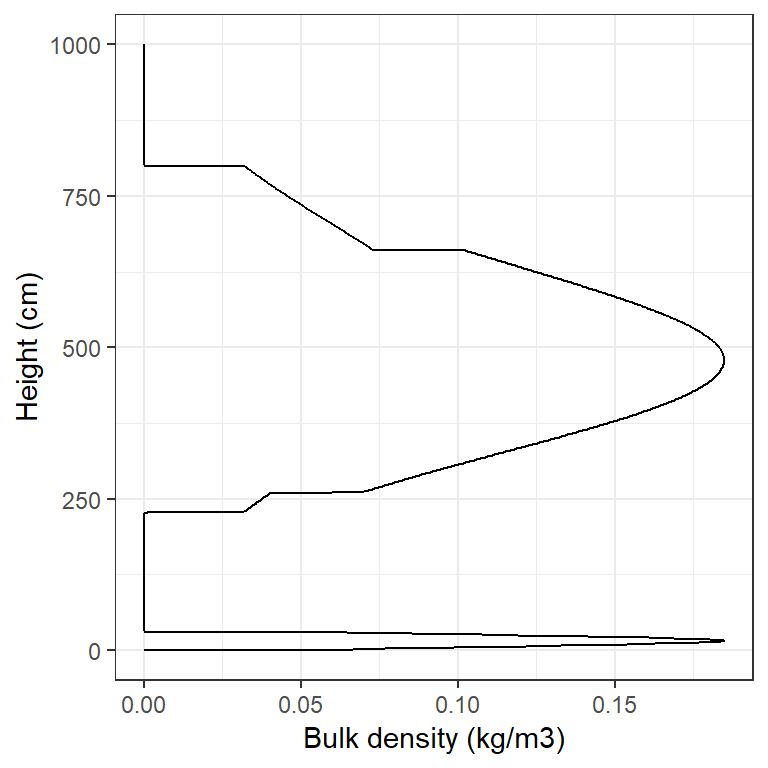
\includegraphics{medfatebook_files/figure-latex/unnamed-chunk-77-1} \end{center}

Let's consider an example for a \emph{Quercus ilex} target tree of 4m height and where species-specific conductivity \(K_{s,max,ref} = 0.77\) is the apical value for trees of \(H_{ref} = 6.6\) m (in \texttt{medfate}, values of \(H_{ref}\) are taken from median height values; see parameter \texttt{Hmed} in \texttt{SpParamsMED}). The corrected conductivity for a tree of height 4 m will be a bit lower than that of the reference height:

\begin{Shaded}
\begin{Highlighting}[]
\NormalTok{xylem_kmax =}\StringTok{ }\FloatTok{0.77}
\NormalTok{H =}\StringTok{ }\DecValTok{400} \CommentTok{# in cm}
\NormalTok{Href =}\StringTok{ }\DecValTok{660} \CommentTok{# in cm}
\NormalTok{f =}\StringTok{ }\KeywordTok{hydraulics_referenceConductivityHeightFactor}\NormalTok{(Href, H);}
\NormalTok{f}
\end{Highlighting}
\end{Shaded}

\begin{verbatim}
## [1] 0.7863352
\end{verbatim}

\begin{Shaded}
\begin{Highlighting}[]
\NormalTok{xylem_kmax_cor =}\StringTok{ }\NormalTok{xylem_kmax }\OperatorTok{*}\StringTok{ }\NormalTok{f}
\NormalTok{xylem_kmax_cor}
\end{Highlighting}
\end{Shaded}

\begin{verbatim}
## [1] 0.6054781
\end{verbatim}

Once the reference conductivity is corrected, the maximum stem conductance without accounting for conduit taper is:
\begin{equation}
k_{s,max, notaper}=\frac{1000}{0.018} \frac{K_{s,max,cor}\cdot A_{s}}{H\cdot A_{l}}
\end{equation}
where \(H\) is the tree height (here in m), \(A_{s}\) is the sapwood area, \(A_{l}\) is the leaf area and 1000/0.018 is a factor used to go from kg to mmol. The ratio \(A_{l}/A_{s} = 1/H_v\) is a fixed species parameter in soil water balance calculations (see parameter \texttt{Al2As}), but becomes variable when simulating plant growth. Let's assume that \emph{Quercus ilex} the leaf to sapwood area ratio is \(A_{l}/A_{s} = 2512\). The maximum (leaf-specific) stem conductance without taper (\(k_{s, max, notaper}\)) for the tree of 4 m height is then:

\begin{Shaded}
\begin{Highlighting}[]
\NormalTok{Al2As =}\StringTok{ }\DecValTok{2512} 

\NormalTok{kstemmax =}\StringTok{ }\KeywordTok{hydraulics_maximumStemHydraulicConductance}\NormalTok{(xylem_kmax, }
\NormalTok{                  Href, Al2As, H, }\DataTypeTok{angiosperm =} \OtherTok{TRUE}\NormalTok{,}\DataTypeTok{taper =} \OtherTok{FALSE}\NormalTok{)}
\NormalTok{kstemmax}
\end{Highlighting}
\end{Shaded}

\begin{verbatim}
## [1] 3.347698
\end{verbatim}

In order to consider taper of xylem conduits we calculate the whole-tree conductance per unit leaf area (\(k_{s, max, taper}\)) as described in \citet{Christoffersen2016}:
\begin{equation}
k_{s, max, taper}=\frac{1000}{0.018} \cdot \frac{K_{s,max,pet}\cdot A_{s}}{H\cdot A_{l}}\cdot \chi_{tap:notap,ag}(H)
\end{equation}
where \(K_{s,max,pet}\) is the conductivity at the petiole level and \(\chi_{tap:notap,ag}(H)\) is the taper factor accounting for the decrease in the xylem conduits diameter with the height, from the petiole to base of the trunk, which mitigates the negative effects of height on the hydraulic safety. The conductivity at the petiole level is obtained from \(K_{s,max,ref}\) using again:
\begin{equation}
K_{s,max,pet} = K_{s,max,ref}\cdot (r_{int, pet}/r_{int,ref})^{2}
\end{equation}
where \(r_{int, pet}\) is the radius of the petiole in the model of \citet{Savage2010}. \citet{Christoffersen2016} use \(r_{int, pet} = 10\) \(\mu m\) but we define it as the radius of apical conduits in a tree of 1 m height:

\begin{Shaded}
\begin{Highlighting}[]
\KeywordTok{hydraulics_terminalConduitRadius}\NormalTok{(}\FloatTok{100.0}\NormalTok{)}
\end{Highlighting}
\end{Shaded}

\begin{verbatim}
## [1] 9.035871
\end{verbatim}

\(\chi_{tap:notap,ag}(H)\) is calculated as described in the Appendix 1 section of \citet{Christoffersen2016} (see also \citet{Savage2010}). The following figure shows the value of \(\chi_{tap:notap,ag}\) for different heights:

\begin{center}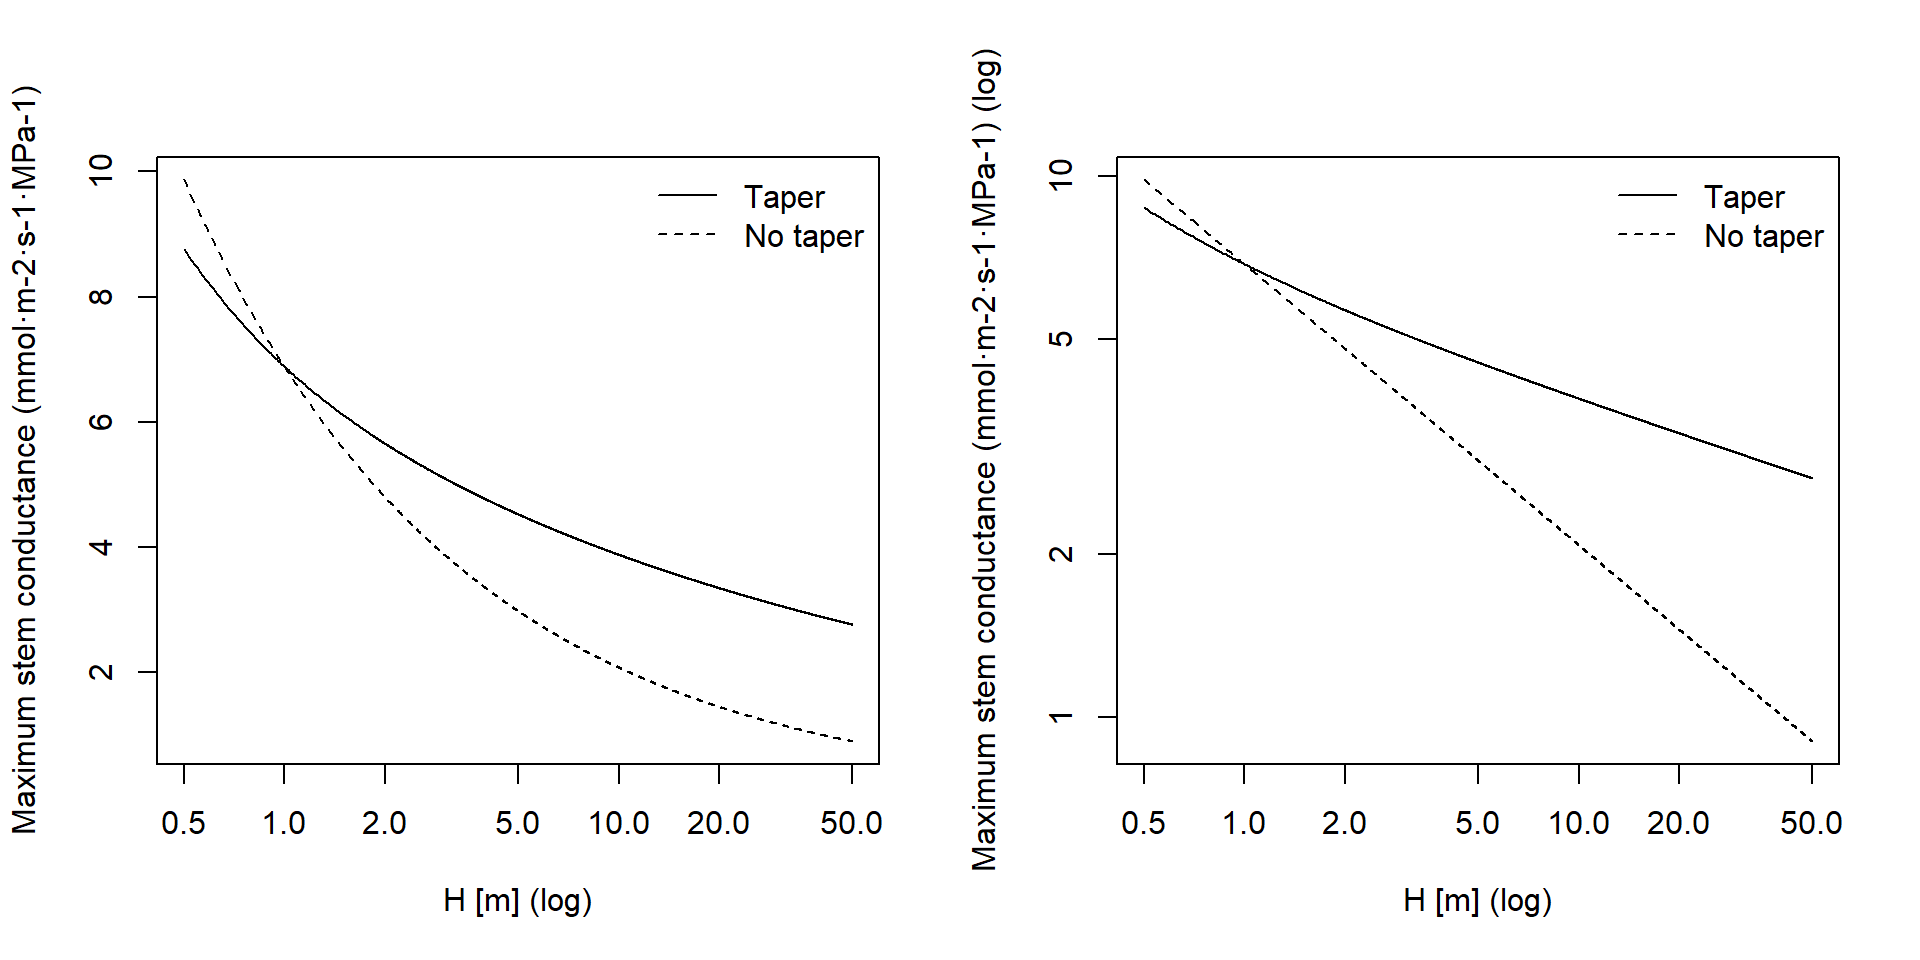
\includegraphics{medfatebook_files/figure-latex/unnamed-chunk-81-1} \end{center}

Note that, since \(\chi_{tap:notap,ag}(1) = 3.82\) (indicated using grey dashed lines in the last figure), the equation of maximum conductance with taper would give a higher conductance than the equation without taper for a tree of 1 m height, which is supposed to have a conductance equal to conductivity. To solve this issue we define the taper factor as \(\chi_{tap:notap,ag}(H)/\chi_{tap:notap,ag}(1)\):
\begin{equation}
k_{s, max, taper}=\frac{1000}{0.018} \cdot \frac{K_{s,max,pet}\cdot A_{s}}{H\cdot A_{l}}\cdot \frac{\chi_{tap:notap,ag}(H)}{\chi_{tap:notap,ag}(1)}
\end{equation}
The maximum stem conductance with taper (\(k_{s, max, taper}\)) of a \emph{Q. ilex} tree of 4 m height, calculated with this second equation, is:

\begin{Shaded}
\begin{Highlighting}[]
\NormalTok{kstemmax_tap =}\StringTok{ }\KeywordTok{hydraulics_maximumStemHydraulicConductance}\NormalTok{(xylem_kmax, }
\NormalTok{                      Href, Al2As, H, }\DataTypeTok{angiosperm =} \OtherTok{TRUE}\NormalTok{, }\DataTypeTok{taper =} \OtherTok{TRUE}\NormalTok{)}
\NormalTok{kstemmax_tap}
\end{Highlighting}
\end{Shaded}

\begin{verbatim}
## [1] 4.764396
\end{verbatim}

The next two plots show the variation of \(k_{s,max}\) for \emph{Q. ilex} depending on the tree height and with/without considering taper of conduits. The plot on the right (both axes in log) show the slope of the dependency of conductance with height in both cases:

\begin{center}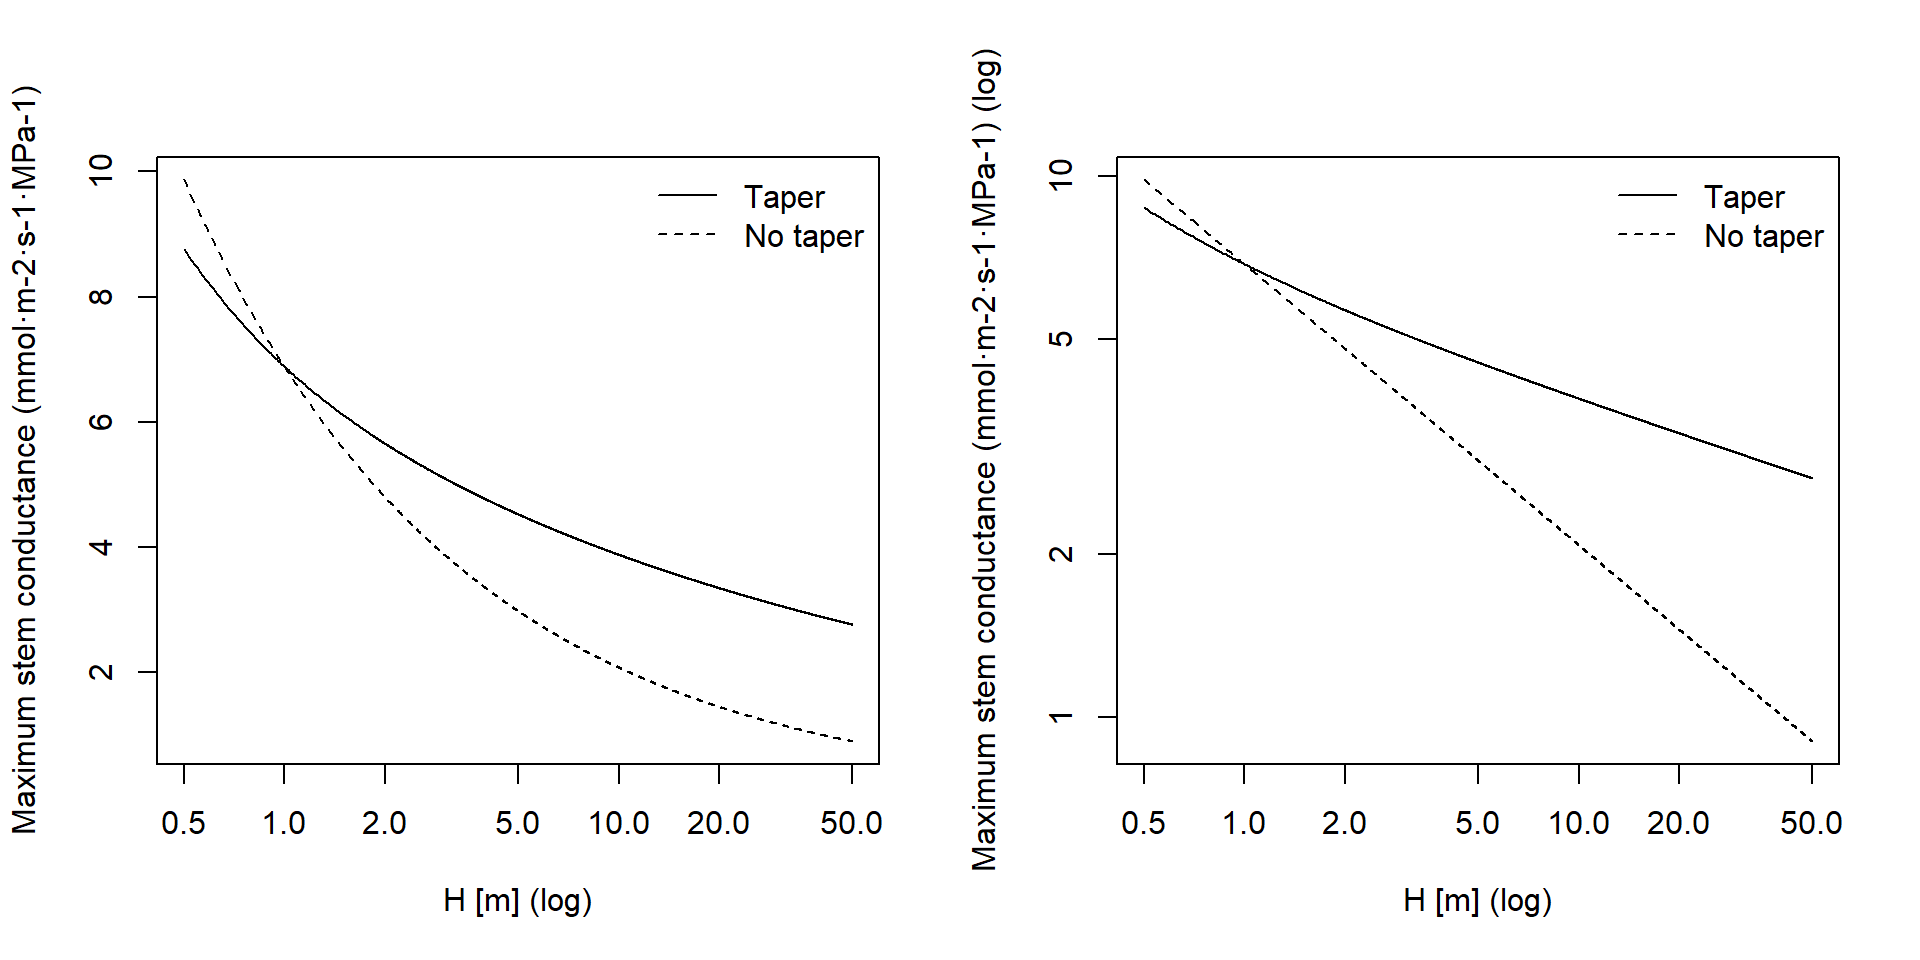
\includegraphics{medfatebook_files/figure-latex/unnamed-chunk-83-1} \end{center}

\hypertarget{root-xylem-maximum-hydraulic-conductance}{%
\subsection{Root xylem maximum hydraulic conductance}\label{root-xylem-maximum-hydraulic-conductance}}

To obtain maximum root xylem conductance (\(k_{r, max}\), in \(mmol \cdot m^{-2} \cdot s^{-1} \cdot MPa^{-1}\)), one option taken by \citet{Christoffersen2016} is to assume that minimum stem resistance (inverse of maximum conductance) represents a fixed proportion of the minimum total tree (stem+root) resistance. A value 0.625 (i.e.~62.5\%) suggested by these authors leads to maximum total tree conductance for our \emph{Q. ilex} tree being:

\begin{Shaded}
\begin{Highlighting}[]
\NormalTok{ktot =}\StringTok{ }\NormalTok{kstemmax}\OperatorTok{*}\FloatTok{0.625}
\NormalTok{ktot}
\end{Highlighting}
\end{Shaded}

\begin{verbatim}
## [1] 2.092311
\end{verbatim}

and the maximum root xylem conductance would be therefore:

\begin{Shaded}
\begin{Highlighting}[]
\NormalTok{krootmax =}\StringTok{ }\DecValTok{1}\OperatorTok{/}\NormalTok{((}\DecValTok{1}\OperatorTok{/}\NormalTok{ktot)}\OperatorTok{-}\NormalTok{(}\DecValTok{1}\OperatorTok{/}\NormalTok{kstemmax))}
\NormalTok{krootmax}
\end{Highlighting}
\end{Shaded}

\begin{verbatim}
## [1] 5.579497
\end{verbatim}

Now, we need to divide total maximum conductance of the root system xylem among soil layers we need weights inversely proportional to the length of transport distances \citep{Sperry2016}. Vertical transport lengths can be calculated from soil depths and radial spread can be calculated assuming cylinders with volume proportional to the proportions of fine root biomass. Let's assume a soil with three layers:

\begin{Shaded}
\begin{Highlighting}[]
\NormalTok{d =}\StringTok{ }\NormalTok{s}\OperatorTok{$}\NormalTok{dVec}
\NormalTok{d}
\end{Highlighting}
\end{Shaded}

\begin{verbatim}
## [1]  300  700 1000
\end{verbatim}

The proportion of fine roots in each layer, assuming a linear dose response model, will be:

\begin{Shaded}
\begin{Highlighting}[]
\NormalTok{Z50 =}\StringTok{ }\DecValTok{200}
\NormalTok{Z95 =}\StringTok{ }\DecValTok{1500}
\NormalTok{v1 =}\StringTok{ }\KeywordTok{root_ldrDistribution}\NormalTok{(Z50,Z95, d)}
\NormalTok{v1}
\end{Highlighting}
\end{Shaded}

\begin{verbatim}
##           [,1]      [,2]       [,3]
## [1,] 0.6661036 0.2784153 0.05548106
\end{verbatim}

Having this information, the calculation of root length (i.e.~the sum of vertical and radial lengths) to each layer (\(L_j\)) is done using function \texttt{root\_rootLength()}:

\begin{Shaded}
\begin{Highlighting}[]
\NormalTok{rl =}\StringTok{ }\KeywordTok{root_rootLengths}\NormalTok{(v1, d)}
\NormalTok{rl}
\end{Highlighting}
\end{Shaded}

\begin{verbatim}
## [1] 2150.000 1496.481 1816.149
\end{verbatim}

where lengths are in mm. The proportion of total root xylem conductance corresponding to each layer (\(w_j\)) is given by \texttt{root\_xylemConductanceProportions()}:

\begin{Shaded}
\begin{Highlighting}[]
\NormalTok{w1 =}\StringTok{ }\KeywordTok{root_xylemConductanceProportions}\NormalTok{(v1, d)}
\NormalTok{w1}
\end{Highlighting}
\end{Shaded}

\begin{verbatim}
## [1] 0.2762029 0.3968217 0.3269754
\end{verbatim}

Xylem conductance proportions can be quite different than the fine root biomass proportions. This is because radial lengths are largest for the first top layers and vertical lengths are largest for the bottom layers. The maximum root xylem conductances of each layer will be the product of maximum total conductance of root xylem and weights:

\begin{Shaded}
\begin{Highlighting}[]
\NormalTok{w1}\OperatorTok{*}\NormalTok{krootmax}
\end{Highlighting}
\end{Shaded}

\begin{verbatim}
## [1] 1.541073 2.214065 1.824358
\end{verbatim}

In \textbf{medfate} we calculate maximum root xylem conductance using a reference root xylem conductivity value (\(K_{r,max,ref}\)):
\begin{equation}
k_{r,max}=\frac{1000}{0.018} \cdot \sum_{j}{\frac{w_j \cdot K_{r,max,ref}\cdot A_{s}}{L_j\cdot A_{l}}}
\end{equation}
where \(w_j\) are root xylem conductance proportion of layer \(j\) and \(L_j\) is the root length (in m) to layer \(j\). Note that here we use weights \(w_j\) assuming they represent proportions of total sapwood area that come from each layer (i.e.~the longer the path the larger the proportion of sapwood area). This calculation is made available by function \texttt{hydraulics\_maximumRootHydraulicConductance()}. When \(K_{r,max,ref}\) is missing, then we assume that \(K_{r,max,ref} = K_{x,max,ref}\). Let's consider the same \emph{Q. ilex} tree of 4m height as before. If we specify root xylem specific conductivity as \(K_{r,max,ref} = K_{s,max,ref} =0.77\) we have:

\begin{Shaded}
\begin{Highlighting}[]
\NormalTok{rootxylem_kmax =}\StringTok{ }\FloatTok{0.77}
\NormalTok{krootmax =}\StringTok{ }\KeywordTok{hydraulics_maximumRootHydraulicConductance}\NormalTok{(rootxylem_kmax, Al2As, }
\NormalTok{                                                      v1, d)}
\NormalTok{krootmax}
\end{Highlighting}
\end{Shaded}

\begin{verbatim}
## [1] 9.769308
\end{verbatim}

The maximum root xylem conductances of each layer would be:

\begin{Shaded}
\begin{Highlighting}[]
\NormalTok{krootmaxvec =}\StringTok{ }\NormalTok{w1}\OperatorTok{*}\NormalTok{krootmax}
\NormalTok{krootmaxvec}
\end{Highlighting}
\end{Shaded}

\begin{verbatim}
## [1] 2.698311 3.876673 3.194324
\end{verbatim}

and the fraction of total xylem resistance due to stem would be:

\begin{Shaded}
\begin{Highlighting}[]
\NormalTok{(}\DecValTok{1}\OperatorTok{/}\NormalTok{kstemmax)}\OperatorTok{/}\NormalTok{((}\DecValTok{1}\OperatorTok{/}\NormalTok{kstemmax)}\OperatorTok{+}\NormalTok{(}\DecValTok{1}\OperatorTok{/}\NormalTok{krootmax))}
\end{Highlighting}
\end{Shaded}

\begin{verbatim}
## [1] 0.7447818
\end{verbatim}

In contrast with the approach of \citet{Christoffersen2016}, in this approach the root maximum conductance depends root length and distribution, and is not a fixed fraction of stem maximum conductance. Assuming constant root length, then the proportion of total resistance due to the stem will increase with tree height \citep{Magnani2000}:

\begin{center}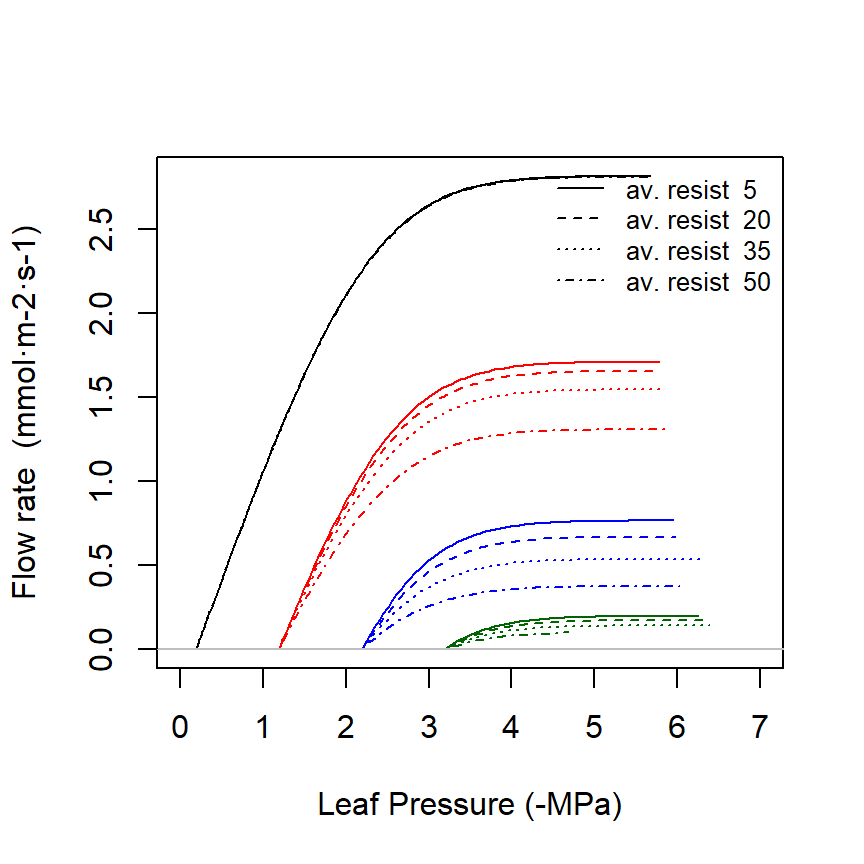
\includegraphics{medfatebook_files/figure-latex/unnamed-chunk-94-1} \end{center}

where the horizontal gray line indicates the value of 62.5\%. Of course rooting depth also increases with tree age, but young trees have higher root-to-shoot ratios than older ones. Hence, a root maximum conductance that is not fixed but increases with age seems a priori more realistic. Moreover, \citet{Christoffersen2016} justify the value of 62.5\% from a study which quantified total aboveground and belowground resistance in tropical trees \citep{Fisher2006} under near-saturated (wet season) conditions, but values of belowground resistance reported in this study for wet conditions and trees of 30 m height are around 13\%, which equals to 87\% fraction of aboveground resistance. On the other hand, while rooting depths are limited by soil depth, lateral root length increases with age and, hence, the model could be made more realistic if this is taken into account and the curve above would probably saturate at lower percentages.

\hypertarget{rhizosphere-maximum-hydraulic-conductance}{%
\subsection{Rhizosphere maximum hydraulic conductance}\label{rhizosphere-maximum-hydraulic-conductance}}

Maximum rhizosphere conductance (\(k_{rh, max}\), in \(mmol \cdot m^{-2} \cdot s^{-1} \cdot MPa^{-1}\)) is difficult to measure directly, as it depends on the rhizosphere (i.e.~fine root) surface in each soil layer, and will probably always be a parameter to be calibrated. Instead of trying to estimate rhizosphere surface from root architecture \citep{Sperry1998}, we follow \citet{Sperry2016a} and determine the maximum rhizosphere conductance in each layer from an inputed `average percentage rhizosphere resistance'. The percentage of continuum resistance corresponding to the rhizosphere is calculated from the vulnerability curves of stem, root and rhizosphere at the same water potential. The average resistance is found by evaluating the percentage for water potential values between 0 and \(\Psi_{crit}\). The following figure illustrates how the supply function, for different soil water potentials, is affected by increasing values of the average percentage of rhizosphere resistance:

\begin{center}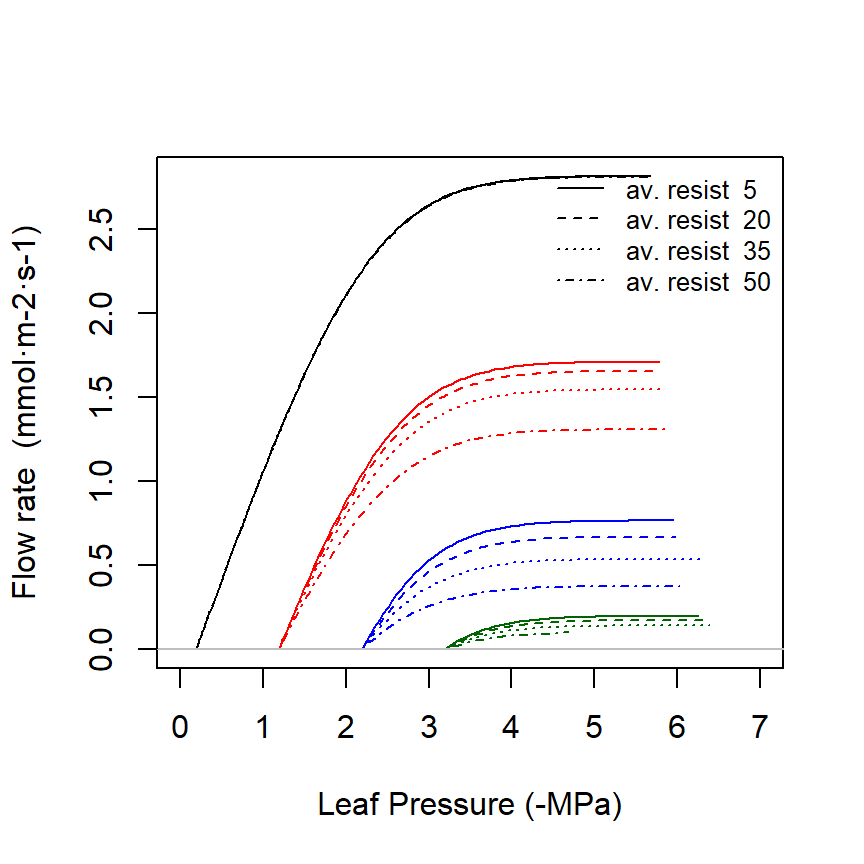
\includegraphics{medfatebook_files/figure-latex/unnamed-chunk-95-1} \end{center}

\citet{Sperry2016a} found average percentages of rhizosphere resistance around 67\%, but these exceptionally-high values were probably a consequence of using an unsegmented supply function (i.e.~single vulnerability curve for roots, stem and leaves). If we specify a 15\% of average resistance in the rhizosphere (see parameter \texttt{averageFracRhizosphereResistance} in function \texttt{defaultControl()}), the maximum rhizosphere conductance values for the three layers are found calling:

\begin{Shaded}
\begin{Highlighting}[]
\NormalTok{krmax =}\StringTok{ }\KeywordTok{rep}\NormalTok{(}\DecValTok{0}\NormalTok{,}\DecValTok{3}\NormalTok{) }
\NormalTok{krmax[}\DecValTok{1}\NormalTok{]=}\StringTok{ }\KeywordTok{hydraulics_findRhizosphereMaximumConductance}\NormalTok{(}\DecValTok{15}\NormalTok{, }
\NormalTok{                     s}\OperatorTok{$}\NormalTok{VG_n[}\DecValTok{1}\NormalTok{],s}\OperatorTok{$}\NormalTok{VG_alpha[}\DecValTok{1}\NormalTok{],}
\NormalTok{                     krootmax, rootc,rootd, }
\NormalTok{                     kstemmax, stemc, stemd,}
\NormalTok{                     kleafmax, leafc, leafd)}
\NormalTok{krmax[}\DecValTok{2}\NormalTok{] =}\StringTok{ }\KeywordTok{hydraulics_findRhizosphereMaximumConductance}\NormalTok{(}\DecValTok{15}\NormalTok{, }
\NormalTok{                      s}\OperatorTok{$}\NormalTok{VG_n[}\DecValTok{2}\NormalTok{],s}\OperatorTok{$}\NormalTok{VG_alpha[}\DecValTok{2}\NormalTok{],}
\NormalTok{                      krootmax, rootc,rootd, }
\NormalTok{                      kstemmax, stemc, stemd,}
\NormalTok{                      kleafmax, leafc, leafd)}
\NormalTok{krmax[}\DecValTok{3}\NormalTok{] =}\StringTok{ }\KeywordTok{hydraulics_findRhizosphereMaximumConductance}\NormalTok{(}\DecValTok{15}\NormalTok{, }
\NormalTok{                      s}\OperatorTok{$}\NormalTok{VG_n[}\DecValTok{3}\NormalTok{],s}\OperatorTok{$}\NormalTok{VG_alpha[}\DecValTok{3}\NormalTok{],}
\NormalTok{                      krootmax, rootc,rootd, }
\NormalTok{                      kstemmax, stemc, stemd,}
\NormalTok{                      kleafmax, leafc, leafd)}
\NormalTok{krmax}
\end{Highlighting}
\end{Shaded}

\begin{verbatim}
## [1] 276438796  97039144  97039144
\end{verbatim}

The values are the same because the texture of the three layers is the same in this case. If we take into account root distribution, actual maximum rhizosphere conductance values are:

\begin{Shaded}
\begin{Highlighting}[]
\NormalTok{krmax}\OperatorTok{*}\NormalTok{v1}
\end{Highlighting}
\end{Shaded}

\begin{verbatim}
##           [,1]     [,2]    [,3]
## [1,] 184136883 27017184 5383835
\end{verbatim}

\hypertarget{pressure-volume-curves-1}{%
\subsection{Pressure-volume curves}\label{pressure-volume-curves-1}}

Parameters of the pressure-volume curve (i.e. \(\pi_{0,stem}\) and \(\epsilon_{stem}\)) for leaf and stem symplastic tissue are required for each species. When parameters for stem tissue are missing, \textbf{medfate} estimates them from wood density following \citet{Christoffersen2016}:
\begin{equation}
\pi_{0,stem} = 0.52 - 4.16 \cdot \rho_{wood}
\end{equation}

\begin{equation}
\epsilon_{stem} = \sqrt{1.02 \cdot e^{8.5\cdot \rho_{wood}}-2.89}
\end{equation}

\hypertarget{plant-water-storage-capacity}{%
\subsection{Plant water storage capacity}\label{plant-water-storage-capacity}}

The water storage capacity of sapwood tissue per leaf area unit (\(V_{sapwood}\); in \(m^3 \cdot m^{-2}\)) can be estimated as the product of stem height (\(H\) in m) and Huber value (\(H_v\); ratio of sapwood area to leaf area in \(m^2 \cdot m^{-2}\)) times a factor to account for the non-cylindrical shape (\url{http://www.fao.org/forestry/17109/en/}):
\begin{equation}
V_{sapwood} = 0.48 \cdot H \cdot H_v \cdot \Theta_{sapwood}
\end{equation}
\(\Theta_{sapwood}\) is sapwood porosity (\(cm^3\) of water per \(cm^3\) of sapwood tissue), which can be estimated from wood density (\(\rho_{wood}\); in \(g \cdot cm^{-3}\)):
\begin{equation}
\Theta_{sapwood} = 1 - (\rho_{wood} / 1.54)
\end{equation}
where the density of wood substance can be assumed to be fixed and equal to 1.54 \(g \cdot cm^{-3}\) \citep{Dunlap1914}. For example, wood densities ranging from 0.443 to 1.000 \(g \cdot cm^{-3}\) result in sapwood porosity values between 0.35 and 0.71.

Water storage capacity of leaf tissue per leaf area unit (\(V_{leaf}\); in \(m^3 \cdot m^{-2}\)) can be estimated as the product of specific leaf area (SLA; in \(m^2 \cdot kg^{-1}\)) and leaf density (\(\rho_{leaf}\); in \(g \cdot cm^{-3}\)):
\begin{equation}
V_{leaf} = \frac{10^{-3}}{SLA \cdot \rho_{leaf}} \cdot \Theta_{leaf}
\end{equation}
\(\Theta_{leaf}\) is leaf porosity (\(cm^3\) of water per \(cm^3\) of leaf tissue), which can be estimated from leaf density:
\begin{equation}
\Theta_{leaf} = 1 - (\rho_{leaf} / 1.54)
\end{equation}
where the density of wood substance can be assumed to be fixed and equal to 1.54 \(g \cdot cm^{-3}\) (Dunlap 1914).

For example, let's calculate the stem and leaf water capacity for a Q. ilex tree of 15 m height:

\begin{Shaded}
\begin{Highlighting}[]
\NormalTok{wd =}\StringTok{ }\FloatTok{1.0}
\NormalTok{Al2As =}\StringTok{ }\DecValTok{2512} 
\NormalTok{H =}\StringTok{ }\DecValTok{1500} \CommentTok{# 15 m}
\KeywordTok{hydraulics_stemWaterCapacity}\NormalTok{(Al2As, H, wd)}
\end{Highlighting}
\end{Shaded}

\begin{verbatim}
## [1] 0.001005046
\end{verbatim}

\begin{Shaded}
\begin{Highlighting}[]
\NormalTok{ld =}\StringTok{ }\FloatTok{0.7}
\NormalTok{SLA =}\StringTok{ }\FloatTok{5.870} 
\KeywordTok{hydraulics_leafWaterCapacity}\NormalTok{(SLA, ld)}
\end{Highlighting}
\end{Shaded}

\begin{verbatim}
## [1] 0.0001327463
\end{verbatim}

\hypertarget{stomatal-regulation-and-photosynthesis}{%
\section{Stomatal regulation and photosynthesis}\label{stomatal-regulation-and-photosynthesis}}

\hypertarget{stomatal-conductance}{%
\subsection{Stomatal conductance}\label{stomatal-conductance}}

Maximum stomatal conductance (\(g_{swmax}\)) is an input parameter for each species. When species-specific values are missing, the following relation with maximum leaf hydraulic conductance (\(k_{l, max}\)) is used \citep{Mencuccini2003}:
\begin{equation}
g_{swmax} = e^{4.797 + 0.633\cdot \log(k_{l, max})}
\end{equation}

Species values for \(g_{swmin}\) were taken from \citet{Duursma2018}. Following the same authors, a value of \(g_{swmin}\) = 0.0045 \(mol H_2O \cdot s^{-1} \cdot m^{-2}\) is taken as default, when species-specific values are missing.

\hypertarget{photosynthesis}{%
\subsection{Photosynthesis}\label{photosynthesis}}

Rubisco's maximum carboxylation rate at 25ºC (\(V_{max, 298}\), in \(\mu mol CO_2 \cdot s^{-1} \cdot m^{-2}\)) is a required input parameter for each species (\texttt{Vmax298}), and if its value is missing a default value of 100 \(\mu mol CO_2 \cdot s^{-1} \cdot m^{-2}\) is used. The maximum rate of electron transport at the same temperature (\(J_{max, 298}\)) can be provided by the user (\texttt{Jmax298}) but, if not, it is estimated from \(V_{max, 298}\) using \citet{Walker2014}:

\begin{equation}
J_{max, 298} = e^{1.197 + 0.847\cdot \log(V_{max,298})}
\end{equation}

\hypertarget{symbols}{%
\chapter{Symbols}\label{symbols}}

The following tables list all symbols used in this document, along with their units and definition. When symbols are input parameters for \textbf{medfate} model functions, the name of those parameters in data frame \texttt{SpParamsMED} is also indicated.

\hypertarget{anatomy}{%
\section{Anatomy}\label{anatomy}}

\begin{longtable}[]{@{}llll@{}}
\toprule
\begin{minipage}[b]{0.11\columnwidth}\raggedright
Symbol\strut
\end{minipage} & \begin{minipage}[b]{0.10\columnwidth}\raggedright
Units\strut
\end{minipage} & \begin{minipage}[b]{0.12\columnwidth}\raggedright
R param\strut
\end{minipage} & \begin{minipage}[b]{0.45\columnwidth}\raggedright
Description\strut
\end{minipage}\tabularnewline
\midrule
\endhead
\begin{minipage}[t]{0.11\columnwidth}\raggedright
\(H_v\)\strut
\end{minipage} & \begin{minipage}[t]{0.10\columnwidth}\raggedright
\(m^2 \cdot m^{-2}\)\strut
\end{minipage} & \begin{minipage}[t]{0.12\columnwidth}\raggedright
\texttt{1/Al2As}\strut
\end{minipage} & \begin{minipage}[t]{0.45\columnwidth}\raggedright
Huber value (ratio of sapwood area to leaf area)\strut
\end{minipage}\tabularnewline
\begin{minipage}[t]{0.11\columnwidth}\raggedright
\(d\)\strut
\end{minipage} & \begin{minipage}[t]{0.10\columnwidth}\raggedright
\(cm\)\strut
\end{minipage} & \begin{minipage}[t]{0.12\columnwidth}\raggedright
\texttt{LeafWidth}\strut
\end{minipage} & \begin{minipage}[t]{0.45\columnwidth}\raggedright
Leaf width\strut
\end{minipage}\tabularnewline
\begin{minipage}[t]{0.11\columnwidth}\raggedright
\(SLA\)\strut
\end{minipage} & \begin{minipage}[t]{0.10\columnwidth}\raggedright
\(m^2 \cdot kg^{-1}\)\strut
\end{minipage} & \begin{minipage}[t]{0.12\columnwidth}\raggedright
\texttt{SLA}\strut
\end{minipage} & \begin{minipage}[t]{0.45\columnwidth}\raggedright
Specific leaf area\strut
\end{minipage}\tabularnewline
\begin{minipage}[t]{0.11\columnwidth}\raggedright
\(\rho_{leaf}\)\strut
\end{minipage} & \begin{minipage}[t]{0.10\columnwidth}\raggedright
\(g \cdot cm^{-3}\)\strut
\end{minipage} & \begin{minipage}[t]{0.12\columnwidth}\raggedright
\texttt{LeafDens}\strut
\end{minipage} & \begin{minipage}[t]{0.45\columnwidth}\raggedright
Leaf tissue density\strut
\end{minipage}\tabularnewline
\begin{minipage}[t]{0.11\columnwidth}\raggedright
\(\rho_{wood}\)\strut
\end{minipage} & \begin{minipage}[t]{0.10\columnwidth}\raggedright
\(g \cdot cm^{-3}\)\strut
\end{minipage} & \begin{minipage}[t]{0.12\columnwidth}\raggedright
\texttt{WoodDens}\strut
\end{minipage} & \begin{minipage}[t]{0.45\columnwidth}\raggedright
Wood tissue density\strut
\end{minipage}\tabularnewline
\begin{minipage}[t]{0.11\columnwidth}\raggedright
\(\Theta_{sapwood}\)\strut
\end{minipage} & \begin{minipage}[t]{0.10\columnwidth}\raggedright
\(m^3 \cdot m^{-3}\)\strut
\end{minipage} & \begin{minipage}[t]{0.12\columnwidth}\raggedright
\strut
\end{minipage} & \begin{minipage}[t]{0.45\columnwidth}\raggedright
Sapwood porosity (volume of empty spaces over total volume)\strut
\end{minipage}\tabularnewline
\begin{minipage}[t]{0.11\columnwidth}\raggedright
\(\Theta_{leaf}\)\strut
\end{minipage} & \begin{minipage}[t]{0.10\columnwidth}\raggedright
\(m^3 \cdot m^{-3}\)\strut
\end{minipage} & \begin{minipage}[t]{0.12\columnwidth}\raggedright
\strut
\end{minipage} & \begin{minipage}[t]{0.45\columnwidth}\raggedright
Leaf porosity (volume of empty spaces over total volume)\strut
\end{minipage}\tabularnewline
\bottomrule
\end{longtable}

\hypertarget{plant-hydraulics-2}{%
\section{Plant hydraulics}\label{plant-hydraulics-2}}

\begin{longtable}[]{@{}llll@{}}
\toprule
\begin{minipage}[b]{0.11\columnwidth}\raggedright
Symbol\strut
\end{minipage} & \begin{minipage}[b]{0.10\columnwidth}\raggedright
Units\strut
\end{minipage} & \begin{minipage}[b]{0.12\columnwidth}\raggedright
R param\strut
\end{minipage} & \begin{minipage}[b]{0.45\columnwidth}\raggedright
Description\strut
\end{minipage}\tabularnewline
\midrule
\endhead
\begin{minipage}[t]{0.11\columnwidth}\raggedright
\(K_{s,max,ref}\)\strut
\end{minipage} & \begin{minipage}[t]{0.10\columnwidth}\raggedright
\(kg \cdot s^{-1} \cdot m^{-1} \cdot MPa^{-1}\)\strut
\end{minipage} & \begin{minipage}[t]{0.12\columnwidth}\raggedright
\texttt{Kmax\_stemxylem}\strut
\end{minipage} & \begin{minipage}[t]{0.45\columnwidth}\raggedright
Maximum stem sapwood reference conductivity per leaf area unit\strut
\end{minipage}\tabularnewline
\begin{minipage}[t]{0.11\columnwidth}\raggedright
\(K_{r,max,ref}\)\strut
\end{minipage} & \begin{minipage}[t]{0.10\columnwidth}\raggedright
\(kg \cdot s^{-1} \cdot m^{-1} \cdot MPa^{-1}\)\strut
\end{minipage} & \begin{minipage}[t]{0.12\columnwidth}\raggedright
\texttt{Kmax\_rootxylem}\strut
\end{minipage} & \begin{minipage}[t]{0.45\columnwidth}\raggedright
Maximum root sapwood reference conductivity per leaf area unit\strut
\end{minipage}\tabularnewline
\begin{minipage}[t]{0.11\columnwidth}\raggedright
\(k_{s, max}\)\strut
\end{minipage} & \begin{minipage}[t]{0.10\columnwidth}\raggedright
\(mmol \cdot s^{-1} \cdot m^{-2} \cdot MPa^{-1}\)\strut
\end{minipage} & \begin{minipage}[t]{0.12\columnwidth}\raggedright
\strut
\end{minipage} & \begin{minipage}[t]{0.45\columnwidth}\raggedright
Maximum whole-stem conductance (per leaf area unit)\strut
\end{minipage}\tabularnewline
\begin{minipage}[t]{0.11\columnwidth}\raggedright
\(k_{r, max}\)\strut
\end{minipage} & \begin{minipage}[t]{0.10\columnwidth}\raggedright
\(mmol \cdot s^{-1} \cdot m^{-2} \cdot MPa^{-1}\)\strut
\end{minipage} & \begin{minipage}[t]{0.12\columnwidth}\raggedright
\strut
\end{minipage} & \begin{minipage}[t]{0.45\columnwidth}\raggedright
Maximum root conductance (per leaf area unit)\strut
\end{minipage}\tabularnewline
\begin{minipage}[t]{0.11\columnwidth}\raggedright
\(k_{rh, max}\)\strut
\end{minipage} & \begin{minipage}[t]{0.10\columnwidth}\raggedright
\(mmol \cdot s^{-1} \cdot m^{-2} \cdot MPa^{-1}\)\strut
\end{minipage} & \begin{minipage}[t]{0.12\columnwidth}\raggedright
\strut
\end{minipage} & \begin{minipage}[t]{0.45\columnwidth}\raggedright
Maximum rhizosphere conductance (per leaf area unit)\strut
\end{minipage}\tabularnewline
\begin{minipage}[t]{0.11\columnwidth}\raggedright
\(k_{l, max}\)\strut
\end{minipage} & \begin{minipage}[t]{0.10\columnwidth}\raggedright
\(mmol \cdot s^{-1} \cdot m^{-2} \cdot MPa^{-1}\)\strut
\end{minipage} & \begin{minipage}[t]{0.12\columnwidth}\raggedright
\texttt{VCleaf\_kmax}\strut
\end{minipage} & \begin{minipage}[t]{0.45\columnwidth}\raggedright
Maximum leaf conductance (per leaf area unit)\strut
\end{minipage}\tabularnewline
\begin{minipage}[t]{0.11\columnwidth}\raggedright
\(c_l\), \(d_l\)\strut
\end{minipage} & \begin{minipage}[t]{0.10\columnwidth}\raggedright
(unitless), MPa\strut
\end{minipage} & \begin{minipage}[t]{0.12\columnwidth}\raggedright
\texttt{VCleaf\_c}, \texttt{VCleaf\_d}\strut
\end{minipage} & \begin{minipage}[t]{0.45\columnwidth}\raggedright
Parameters of the vulnerability curve for leaves\strut
\end{minipage}\tabularnewline
\begin{minipage}[t]{0.11\columnwidth}\raggedright
\(c_r\), \(d_r\)\strut
\end{minipage} & \begin{minipage}[t]{0.10\columnwidth}\raggedright
(unitless), MPa\strut
\end{minipage} & \begin{minipage}[t]{0.12\columnwidth}\raggedright
\texttt{VCroot\_c}, \texttt{VCroot\_d}\strut
\end{minipage} & \begin{minipage}[t]{0.45\columnwidth}\raggedright
Parameters of the vulnerability curve for root xylem\strut
\end{minipage}\tabularnewline
\begin{minipage}[t]{0.11\columnwidth}\raggedright
\(c_s\), \(d_s\)\strut
\end{minipage} & \begin{minipage}[t]{0.10\columnwidth}\raggedright
(unitless), MPa\strut
\end{minipage} & \begin{minipage}[t]{0.12\columnwidth}\raggedright
\texttt{VCstem\_c}, \texttt{VCstem\_d}\strut
\end{minipage} & \begin{minipage}[t]{0.45\columnwidth}\raggedright
Parameters of the vulnerability curve for stem xylem\strut
\end{minipage}\tabularnewline
\begin{minipage}[t]{0.11\columnwidth}\raggedright
\(n\), \(\alpha\)\strut
\end{minipage} & \begin{minipage}[t]{0.10\columnwidth}\raggedright
\strut
\end{minipage} & \begin{minipage}[t]{0.12\columnwidth}\raggedright
\strut
\end{minipage} & \begin{minipage}[t]{0.45\columnwidth}\raggedright
Texture-specific parameters of the van Genuchten equation\strut
\end{minipage}\tabularnewline
\begin{minipage}[t]{0.11\columnwidth}\raggedright
\(\Psi\)\strut
\end{minipage} & \begin{minipage}[t]{0.10\columnwidth}\raggedright
MPa\strut
\end{minipage} & \begin{minipage}[t]{0.12\columnwidth}\raggedright
\strut
\end{minipage} & \begin{minipage}[t]{0.45\columnwidth}\raggedright
Water potential in a given water compartment\strut
\end{minipage}\tabularnewline
\begin{minipage}[t]{0.11\columnwidth}\raggedright
\(\Psi_P\)\strut
\end{minipage} & \begin{minipage}[t]{0.10\columnwidth}\raggedright
MPa\strut
\end{minipage} & \begin{minipage}[t]{0.12\columnwidth}\raggedright
\strut
\end{minipage} & \begin{minipage}[t]{0.45\columnwidth}\raggedright
Turgor water potential in a given water compartment\strut
\end{minipage}\tabularnewline
\begin{minipage}[t]{0.11\columnwidth}\raggedright
\(\Psi_S\)\strut
\end{minipage} & \begin{minipage}[t]{0.10\columnwidth}\raggedright
MPa\strut
\end{minipage} & \begin{minipage}[t]{0.12\columnwidth}\raggedright
\strut
\end{minipage} & \begin{minipage}[t]{0.45\columnwidth}\raggedright
Osmotic (solute) water potential in a given water compartment\strut
\end{minipage}\tabularnewline
\begin{minipage}[t]{0.11\columnwidth}\raggedright
\(\Psi_{cav}\)\strut
\end{minipage} & \begin{minipage}[t]{0.10\columnwidth}\raggedright
MPa\strut
\end{minipage} & \begin{minipage}[t]{0.12\columnwidth}\raggedright
\strut
\end{minipage} & \begin{minipage}[t]{0.45\columnwidth}\raggedright
Minimum water potential experienced by xylem in previous steps (cavitation)\strut
\end{minipage}\tabularnewline
\begin{minipage}[t]{0.11\columnwidth}\raggedright
\(\Psi_{canopy}\)\strut
\end{minipage} & \begin{minipage}[t]{0.10\columnwidth}\raggedright
MPa\strut
\end{minipage} & \begin{minipage}[t]{0.12\columnwidth}\raggedright
\strut
\end{minipage} & \begin{minipage}[t]{0.45\columnwidth}\raggedright
Canopy water potential\strut
\end{minipage}\tabularnewline
\begin{minipage}[t]{0.11\columnwidth}\raggedright
\(\Psi_{leaf}\)\strut
\end{minipage} & \begin{minipage}[t]{0.10\columnwidth}\raggedright
MPa\strut
\end{minipage} & \begin{minipage}[t]{0.12\columnwidth}\raggedright
\strut
\end{minipage} & \begin{minipage}[t]{0.45\columnwidth}\raggedright
Leaf water potential\strut
\end{minipage}\tabularnewline
\begin{minipage}[t]{0.11\columnwidth}\raggedright
\(\Psi_{rootcrown}\)\strut
\end{minipage} & \begin{minipage}[t]{0.10\columnwidth}\raggedright
MPa\strut
\end{minipage} & \begin{minipage}[t]{0.12\columnwidth}\raggedright
\strut
\end{minipage} & \begin{minipage}[t]{0.45\columnwidth}\raggedright
Water potential at the root crown\strut
\end{minipage}\tabularnewline
\begin{minipage}[t]{0.11\columnwidth}\raggedright
\(\Psi_{stem}\)\strut
\end{minipage} & \begin{minipage}[t]{0.10\columnwidth}\raggedright
MPa\strut
\end{minipage} & \begin{minipage}[t]{0.12\columnwidth}\raggedright
\strut
\end{minipage} & \begin{minipage}[t]{0.45\columnwidth}\raggedright
Water potential at the end (highest part) of the stem\strut
\end{minipage}\tabularnewline
\begin{minipage}[t]{0.11\columnwidth}\raggedright
\(PLC\)\strut
\end{minipage} & \begin{minipage}[t]{0.10\columnwidth}\raggedright
{[}0-1{]}\strut
\end{minipage} & \begin{minipage}[t]{0.12\columnwidth}\raggedright
\strut
\end{minipage} & \begin{minipage}[t]{0.45\columnwidth}\raggedright
Proportion of conductance loss in stem xylem tissue\strut
\end{minipage}\tabularnewline
\begin{minipage}[t]{0.11\columnwidth}\raggedright
\(p_{root}\)\strut
\end{minipage} & \begin{minipage}[t]{0.10\columnwidth}\raggedright
{[}0-1{]}\strut
\end{minipage} & \begin{minipage}[t]{0.12\columnwidth}\raggedright
\texttt{pRootDisc}\strut
\end{minipage} & \begin{minipage}[t]{0.45\columnwidth}\raggedright
Relative root conductance leading to hydraulic disconnection from a soil layer\strut
\end{minipage}\tabularnewline
\bottomrule
\end{longtable}

\hypertarget{plant-water-compartments}{%
\section{Plant water compartments}\label{plant-water-compartments}}

\begin{longtable}[]{@{}llll@{}}
\toprule
\begin{minipage}[b]{0.11\columnwidth}\raggedright
Symbol\strut
\end{minipage} & \begin{minipage}[b]{0.10\columnwidth}\raggedright
Units\strut
\end{minipage} & \begin{minipage}[b]{0.12\columnwidth}\raggedright
R param\strut
\end{minipage} & \begin{minipage}[b]{0.45\columnwidth}\raggedright
Description\strut
\end{minipage}\tabularnewline
\midrule
\endhead
\begin{minipage}[t]{0.11\columnwidth}\raggedright
\(\epsilon_{leaf}\)\strut
\end{minipage} & \begin{minipage}[t]{0.10\columnwidth}\raggedright
MPa\strut
\end{minipage} & \begin{minipage}[t]{0.12\columnwidth}\raggedright
\texttt{LeafEPS}\strut
\end{minipage} & \begin{minipage}[t]{0.45\columnwidth}\raggedright
Modulus of elasticity of leaves\strut
\end{minipage}\tabularnewline
\begin{minipage}[t]{0.11\columnwidth}\raggedright
\(\epsilon_{stem}\)\strut
\end{minipage} & \begin{minipage}[t]{0.10\columnwidth}\raggedright
MPa\strut
\end{minipage} & \begin{minipage}[t]{0.12\columnwidth}\raggedright
\texttt{StemEPS}\strut
\end{minipage} & \begin{minipage}[t]{0.45\columnwidth}\raggedright
Modulus of elasticity of symplastic xylem tissue\strut
\end{minipage}\tabularnewline
\begin{minipage}[t]{0.11\columnwidth}\raggedright
\(\pi_{0,leaf}\)\strut
\end{minipage} & \begin{minipage}[t]{0.10\columnwidth}\raggedright
MPa\strut
\end{minipage} & \begin{minipage}[t]{0.12\columnwidth}\raggedright
\texttt{LeafPI0}\strut
\end{minipage} & \begin{minipage}[t]{0.45\columnwidth}\raggedright
Osmotic potential at full turgor of leaves\strut
\end{minipage}\tabularnewline
\begin{minipage}[t]{0.11\columnwidth}\raggedright
\(\pi_{0,stem}\)\strut
\end{minipage} & \begin{minipage}[t]{0.10\columnwidth}\raggedright
MPa\strut
\end{minipage} & \begin{minipage}[t]{0.12\columnwidth}\raggedright
\texttt{StemPI0}\strut
\end{minipage} & \begin{minipage}[t]{0.45\columnwidth}\raggedright
Osmotic potential at full turgor of symplastic xylem tissue\strut
\end{minipage}\tabularnewline
\begin{minipage}[t]{0.11\columnwidth}\raggedright
\(RWC\)\strut
\end{minipage} & \begin{minipage}[t]{0.10\columnwidth}\raggedright
{[}0-1{]}\strut
\end{minipage} & \begin{minipage}[t]{0.12\columnwidth}\raggedright
\strut
\end{minipage} & \begin{minipage}[t]{0.45\columnwidth}\raggedright
Relative water content\strut
\end{minipage}\tabularnewline
\begin{minipage}[t]{0.11\columnwidth}\raggedright
\(RWC_{sym}\)\strut
\end{minipage} & \begin{minipage}[t]{0.10\columnwidth}\raggedright
{[}0-1{]}\strut
\end{minipage} & \begin{minipage}[t]{0.12\columnwidth}\raggedright
\strut
\end{minipage} & \begin{minipage}[t]{0.45\columnwidth}\raggedright
Relative water content in the symplasm fraction of a tissue\strut
\end{minipage}\tabularnewline
\begin{minipage}[t]{0.11\columnwidth}\raggedright
\(RWC_{apo}\)\strut
\end{minipage} & \begin{minipage}[t]{0.10\columnwidth}\raggedright
{[}0-1{]}\strut
\end{minipage} & \begin{minipage}[t]{0.12\columnwidth}\raggedright
\strut
\end{minipage} & \begin{minipage}[t]{0.45\columnwidth}\raggedright
Relative water content in the apoplasm fraction of a tissue\strut
\end{minipage}\tabularnewline
\begin{minipage}[t]{0.11\columnwidth}\raggedright
\(V_{segment}\)\strut
\end{minipage} & \begin{minipage}[t]{0.10\columnwidth}\raggedright
\(m^3 \cdot m^{-2}\)\strut
\end{minipage} & \begin{minipage}[t]{0.12\columnwidth}\raggedright
\strut
\end{minipage} & \begin{minipage}[t]{0.45\columnwidth}\raggedright
Water capacity of a segment (leaf or stem)\strut
\end{minipage}\tabularnewline
\begin{minipage}[t]{0.11\columnwidth}\raggedright
\(V_{leaf}\)\strut
\end{minipage} & \begin{minipage}[t]{0.10\columnwidth}\raggedright
\(m^3 \cdot m^{-2}\)\strut
\end{minipage} & \begin{minipage}[t]{0.12\columnwidth}\raggedright
\strut
\end{minipage} & \begin{minipage}[t]{0.45\columnwidth}\raggedright
Leaf water capacity per leaf area unit\strut
\end{minipage}\tabularnewline
\begin{minipage}[t]{0.11\columnwidth}\raggedright
\(V_{sapwood}\)\strut
\end{minipage} & \begin{minipage}[t]{0.10\columnwidth}\raggedright
\(m^3 \cdot m^{-2}\)\strut
\end{minipage} & \begin{minipage}[t]{0.12\columnwidth}\raggedright
\strut
\end{minipage} & \begin{minipage}[t]{0.45\columnwidth}\raggedright
Sapwood water capacity per leaf area unit\strut
\end{minipage}\tabularnewline
\bottomrule
\end{longtable}

\hypertarget{stomatal-regulation-and-photosynthesis-1}{%
\section{Stomatal regulation and photosynthesis}\label{stomatal-regulation-and-photosynthesis-1}}

\begin{longtable}[]{@{}llll@{}}
\toprule
\begin{minipage}[b]{0.11\columnwidth}\raggedright
Symbol\strut
\end{minipage} & \begin{minipage}[b]{0.10\columnwidth}\raggedright
Units\strut
\end{minipage} & \begin{minipage}[b]{0.12\columnwidth}\raggedright
R param\strut
\end{minipage} & \begin{minipage}[b]{0.45\columnwidth}\raggedright
Description\strut
\end{minipage}\tabularnewline
\midrule
\endhead
\begin{minipage}[t]{0.11\columnwidth}\raggedright
\(g_{swmin}\)\strut
\end{minipage} & \begin{minipage}[t]{0.10\columnwidth}\raggedright
\(mol H_2O \cdot s^{-1} \cdot m^{-2}\)\strut
\end{minipage} & \begin{minipage}[t]{0.12\columnwidth}\raggedright
\texttt{Gwmin}\strut
\end{minipage} & \begin{minipage}[t]{0.45\columnwidth}\raggedright
Minimum stomatal conductance to water vapour\strut
\end{minipage}\tabularnewline
\begin{minipage}[t]{0.11\columnwidth}\raggedright
\(g_{swmax}\)\strut
\end{minipage} & \begin{minipage}[t]{0.10\columnwidth}\raggedright
\(mol H_2O \cdot s^{-1} \cdot m^{-2}\)\strut
\end{minipage} & \begin{minipage}[t]{0.12\columnwidth}\raggedright
\texttt{Gwmax}\strut
\end{minipage} & \begin{minipage}[t]{0.45\columnwidth}\raggedright
Maximum stomatal conductance to water vapour\strut
\end{minipage}\tabularnewline
\begin{minipage}[t]{0.11\columnwidth}\raggedright
\(J_{max, 298}\)\strut
\end{minipage} & \begin{minipage}[t]{0.10\columnwidth}\raggedright
\(\mu mol electrons \cdot m^{-2} \cdot s^{-1}\)\strut
\end{minipage} & \begin{minipage}[t]{0.12\columnwidth}\raggedright
\texttt{Jmax298}\strut
\end{minipage} & \begin{minipage}[t]{0.45\columnwidth}\raggedright
Maximum rate of electron transport at 298K\strut
\end{minipage}\tabularnewline
\begin{minipage}[t]{0.11\columnwidth}\raggedright
\(V_{max, 298}\)\strut
\end{minipage} & \begin{minipage}[t]{0.10\columnwidth}\raggedright
\(\mu mol CO_2 \cdot s^{-1} \cdot m^{-2}\)\strut
\end{minipage} & \begin{minipage}[t]{0.12\columnwidth}\raggedright
\texttt{Vmax298}\strut
\end{minipage} & \begin{minipage}[t]{0.45\columnwidth}\raggedright
Rubisco's maximum carboxylation rate at 298K\strut
\end{minipage}\tabularnewline
\bottomrule
\end{longtable}

\bibliography{medfatebook.bib}


\end{document}
